\documentclass{book}
\usepackage[utf8]{inputenc}
\usepackage[T5]{fontenc}
\usepackage{multirow}
\usepackage[vietnamese]{babel} 
\usepackage[letterpaper,top=2cm,bottom=2cm,left=3cm,right=3cm,marginparwidth=1.75cm]{geometry}
\usepackage{fancyhdr}
\usepackage{bbm}
\pagestyle{fancy}
\fancyhf{} % Xóa nội dung mặc định
\fancyfoot[C]{\thepage} % Số trang ở giữa chân trang
\newtheorem{example}{Example}
\usepackage{amsmath}
\usepackage{amssymb}
\usepackage{graphicx}
\usepackage{float}
\usepackage{enumitem}
\usepackage{subcaption}
\usepackage{tikz}
\usepackage{pgf-pie}
\usepackage{algorithm}
\usepackage{algorithmic}
\usepackage{enumitem} 
\usepackage{multicol}
\usepackage{booktabs}
\usepackage{listings}
\usepackage[x11names]{xcolor}
\usepackage[colorlinks=true, allcolors=blue]{hyperref}
\setlength{\parindent}{0pt}
\setlistdepth{9}
\setcounter{tocdepth}{3}
\setcounter{secnumdepth}{3}

\renewcommand{\familydefault}{\sfdefault}
\renewcommand{\algorithmicrequire}{\textbf{Input:}}
\renewcommand{\algorithmicensure}{\textbf{Output:}}
\renewcommand{\algorithmicif}{\textbf{if}}
\renewcommand{\algorithmicthen}{\textbf{then}}
\renewcommand{\algorithmicelse}{\textbf{else}}
\renewcommand{\algorithmicfor}{\textbf{for}}
\renewcommand{\algorithmicdo}{\textbf{do}}
\renewcommand{\algorithmicend}{\textbf{end}}
\renewcommand{\algorithmiccomment}[1]{/* \texttt{#1} */}
\makeatletter
\newcommand{\SWITCH}[1]{\STATE \textbf{switch} #1 \textbf{do}\begin{ALC@g}}
\newcommand{\ENDSWITCH}{\end{ALC@g}\STATE \textbf{end switch}}
\newcommand{\CASE}[1]{\STATE \textbf{case} #1 \textbf{do} \begin{ALC@g}}
\newcommand{\ENDCASE}{\end{ALC@g}\STATE \textbf{end case}}
\newcommand{\CASELINE}[1]{\STATE \textbf{case} #1\textbf{do} }
\newcommand{\DEFAULT}{\STATE \textbf{case default do:} \begin{ALC@g}}
\newcommand{\ENDDEFAULT}{\end{ALC@g}\STATE \textbf{end default case}}
\newcommand{\DEFAULTLINE}[1]{\STATE \textbf{default case:} }
\makeatother

\title{CS410 - Mạng neural và thuật giải di truyền}
\author{} % It's good practice to add an author or leave it blank
\date{}   % Hides the date

\begin{document}

\maketitle
% 2 - 4 - 9.1 - 9.2 - 12,13.10 - 12,13.11
\tableofcontents
\lstdefinestyle{mystyle}{
    backgroundcolor=\color{black!5},  
    commentstyle=\color{green!40!black},
    keywordstyle=\color{blue},
    numberstyle=\footnotesize\color{gray}, 
    stringstyle=\color{purple},
    basicstyle=\ttfamily\footnotesize,
    breakatwhitespace=false,
    breaklines=true,
    captionpos=b,
    keepspaces=true,
    numbers=left,
    numbersep=10pt,
    showspaces=false,
    showstringspaces=false,
    showtabs=false,
    tabsize=2, 
    frame=single,
    rulecolor=\color{black!30},
    morekeywords={plt, np, figure, arange} 
}

\lstset{style=mystyle}
\chapter{Thuật giải di truyền (Genetic Algorithm)}
\section{Giải thuật di truyền cổ điển}

\subsection{Tối ưu hoá (Optimization)}

\subsubsection{Tối thiểu hoá (minimization)}
Cho hàm số $f: S \to \mathbb{R}$. \\
Tìm $x^* \in S$ sao cho $\forall x \in S, f(x^*) \le f(x)$.

\subsubsection{Tối đa hoá (maximization)}
Cho hàm số $f: S \to \mathbb{R}$. \\
Tìm $x^* \in S$ sao cho $\forall x \in S, f(x^*) \ge f(x)$.

\subsection*{Ví dụ 1:} % Dùng \subsection* để không đánh số phụ
Cho hàm số $f(x) = (x - 0.5)^2$.
Tìm giá trị nhỏ nhất của $f$ trên $\mathbb{R}$.

\textbf{Cách giải:} Tính đạo hàm (derivative) của $f$.

\subsection*{Ví dụ 2:} % Dùng \subsection* để không đánh số phụ
Cho đồ thị $G(V,E)$ biểu diễn độ dài đường đi giữa các thành
phố. Tìm đường đi ngắn nhất giữa 2 thành phố

\textbf{Cách giải:} Thuật toán $Dijkstra$.

\centering
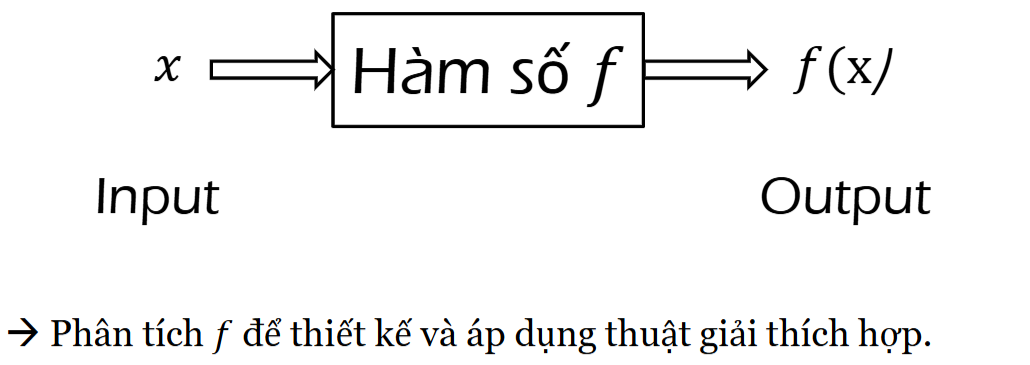
\includegraphics[width=0.6\textwidth]{images/image.png}

\centering
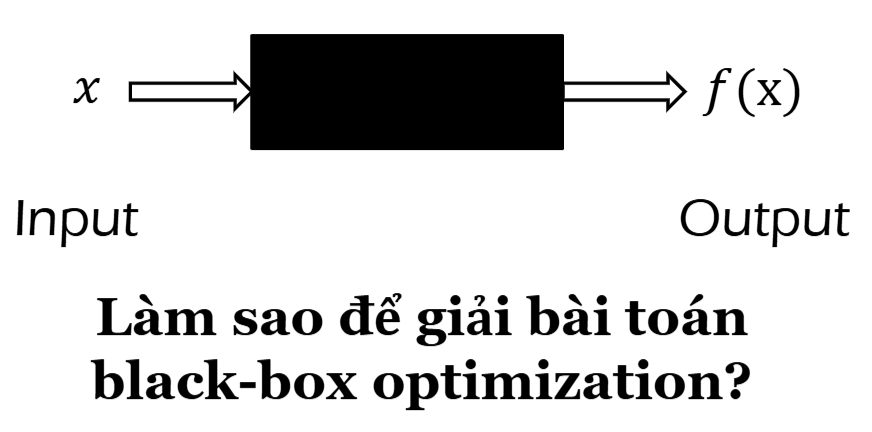
\includegraphics[width=0.6\textwidth]{images/blackbox.png}

\section*{Thách thức khi giải bài toán tối ưu hoá trong thực tế} % Dùng \section* để không đánh số
\begin{itemize}
    \item Thông tin vấn đề không có sẵn, không đầy đủ.
    \item Vấn đề có độ phức tạp cao, khó phân tích.
    \item Chưa có (hoặc không tồn tại) thuật toán hiệu quả.
\end{itemize}

\flushleft
\subsection{Tiến hoá (Evolution)}
\begin{itemize}
    \item Quá trình tiến hoá của các loài trong tự nhiên có nét tương đồng với một quá trình tối ưu hoá
    \item Nhìn chung, sau mỗi thế hệ (generation), các cá thể (individuals) được sinh ra có độ thích nghi (fitness) tốt hơn với môi trường sống.
    \item Tại sao ta có thể lấy ý tưởng từ quá trình tiến hoá để thiết kế thuật giải cho các bài toán tối ưu hoá?
\end{itemize}

Tiến hoá diễn ra trên một quần thể (population) gồm nhiều
cá thể (individual). Mỗi thế hệ nhiều cá thể con được sinh ra.
\begin{itemize}
    \item Tiến hoá đã tạo ra nhiều sinh vật có độ phức tạp cao (Tính
    hữu hiệu – effectiveness).
    \item “Xử lý song song”, nhiều lựa chọn có thể được thử nghiệm
    cùng lúc (Tính hiệu quả – 
    efficiency).
    \item Nếu một vài cá thể thất bại, quá trình tiến hoá vẫn diễn ra
    (Tính bền vững – robustness).
    \item Ý tưởng tổng quát đơn giản, dễ tuỳ biến (Tính đơn giản –
    simplicity).
\end{itemize}

\section*{Các thuật toán tiến hoá (Evolutionary Algorithms)}

Cho hàm số $f: S \rightarrow \mathbb{R}$. \\
Tìm $x^* \in S$ sao cho $\forall x \in S, f(x^*) \ge f(x)$.

\begin{tabular}{|p{0.45\textwidth}|p{0.45\textwidth}|}
\hline
\textbf{Tối ưu hoá} & \textbf{Thuật toán tiến hoá} \\
\hline
$f$ là hàm mục tiêu (objective function) / hàm tối ưu (optimization function). & $f^{EA}$ là hàm thích nghi (fitness function) / hàm lượng giá (evaluation function). \\
\hline
Mỗi $x$ là một lời giải / giải pháp (solution). $x^*$ là (một) giải pháp tối ưu. & Mỗi $x^{EA}$ là một cá thể, hay còn gọi là kiểu gen (genotype). $x$ được xem như là kiểu hình (phenotype). \\
\hline
$S$ là tập tất cả những giải pháp hợp lệ (set of feasible solutions) của bài toán. & $S^{EA}$ là không gian tìm kiếm hợp lệ (feasible search space) của thuật toán. \\
\hline
\end{tabular}

\subsection{Các thuật toán tiến hoá (Evolutionary Algorithms)}
Nhìn chung các thuật toán tiến hoá (Evolutionary Algorithms
– EAs) có 3 thành phần chính:

\begin{itemize}
    \item \textbf{Quần thể} (population) gồm nhiều cá thể (individuals).
    \item Phép \textbf{biến đổi} (variation): để sinh ra cá thể mới (offspring).
    \item Phép \textbf{chọn lọc} (selection): để lựa chọn những cá thể có độ thích nghi (fitness) tốt hơn cho thế hệ tiếp theo.
\end{itemize}

\begin{figure}[H]
    \centering 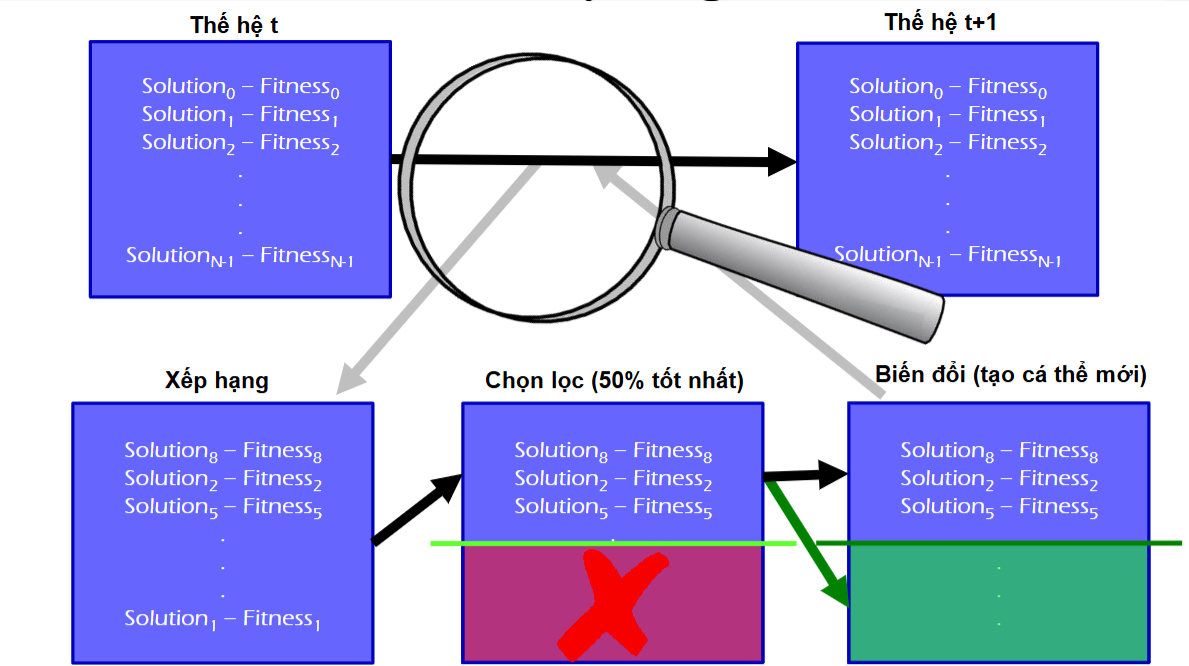
\includegraphics[width=1\linewidth]{images/evo_algo_example.png}
\end{figure}

\subsubsection{Các thuật toán tiến hoá (Cổ điển)}

\begin{itemize}
    \item Kiểu gen là các chuỗi nhị phân (binary strings): \\ 01000110, 1011100, 11100101,...
    \begin{itemize}
        \item[] $\triangleright$ Thuật giải di truyền (Genetic Algorithm) cổ điển.
    \end{itemize}
    \item Kiểu gen là các vector số thực (real-valued vectors): \\ (0.413, 1.313, 0.92), (1.521, 2.1843, 0.12),...
    \begin{itemize}
        \item[] $\triangleright$ Chiến lược tiến hoá (Evolution Strategy) cổ điển.
    \end{itemize}
    \item Kiểu gen là các cấu trúc cây (tree structures), biểu diễn các chương trình / hàm số.
    \begin{itemize}
        \item[] $\triangleright$ Lập trình di truyền (Genetic Programming).
    \end{itemize}
\end{itemize}

\subsubsection{Các thuật toán tiến hoá với mô hình (Model-Based EAs)}

\begin{itemize}
    \item Estimation-of-Distribution Algorithms
    \begin{itemize}
        \item[] $\triangleright$ Extended Compact Genetic Algorithms (ECGA)
        \item[] $\triangleright$ Bayesian Optimization Algorithm (BOA)
        \item[] $\triangleright$ Covariance Matrix Adaptation Evolution Strategy (CMA-ES)
        \item[] $\triangleright$ Adapted Maximum-Likelihood Gaussian Model Iterated Density Estimation Evolutionary Algorithm (AMaLGaM)
        \item[] $\triangleright$ Gene-pool Optimal Mixing Evolution Algorithms (GOMEA) / Linkage Tree Genetic Algorithm (LTGA).
        \item ...
    \end{itemize}
\end{itemize}

\subsubsection{Các thuật toán lấy cảm hứng từ sinh học (bio-inspired)}

\begin{itemize}
    \item[] $\triangleright$ Particle Swarm Optimization (PSO)
    \item[] $\triangleright$ Ant Colony Optimization (ACO)
    \item[] $\triangleright$ Differential Evolution (DE)
    \item[] $\triangleright$ Artificial Immune System (AIS)
    \item[] $\triangleright$ Artificial Bee Colony Algorithm (ABC)
    \item[] $\triangleright$ ...
\end{itemize}

\section*{Lưu ý} % Sử dụng \section* để tạo tiêu đề không đánh số lớn hơn

\begin{itemize}
    \item Hầu hết các thuật toán tiến hoá đều có 3 thành phần chính:
    \begin{enumerate}
        \item Một quần thể.
        \item Một phép biến đổi.
        \item Một phép chọn lọc.
    \end{enumerate}
    \item Mục tiêu của các thuật toán tiến hoá là để giải bài toán cần giải quyết, \textbf{KHÔNG} phải để mô phỏng các hiện tượng tự nhiên.
    \item Các thuật ngữ sinh học được sử dụng để tiện cho việc trao đổi ý tưởng trong nghiên cứu và ứng dụng $\rightarrow$ tránh lạm dụng.
\end{itemize}

\subsection{Thuật giải di truyền (Genetic Algorithm)}

\begin{itemize}
    \item Được đề xuất bởi John Holland (1975).
    \item Kiểu gen là các chuỗi nhị phân (binary strings) có chiều dài cố định $l$.
\end{itemize}

\begin{enumerate}
    \item $t \leftarrow 0$
    \item $P^t \leftarrow \text{initializeAndEvaluateInitialIndividuals}( n )$
    \item \textbf{while} $\text{terminationCriteriaNotSatisfied}( P^t )$ \textbf{do}
    \begin{enumerate}
        \item $S^t \leftarrow \text{selectParents}( P^t, n )$
        \item $O^t \leftarrow \text{createAndEvaluateOffspring}( S^t, n )$
        \item $P^{t+1} \leftarrow O^t$
        \item $t \leftarrow t + 1$
    \end{enumerate}
\end{enumerate}

\subsection{Khởi tạo quần thể
(Population Initialization)}

Quần thể đầu tiên thường được khởi tạo một cách ngẫu
nhiên với phân bố đồng nhất (uniformly random).
\begin{figure}[H]
    \centering
    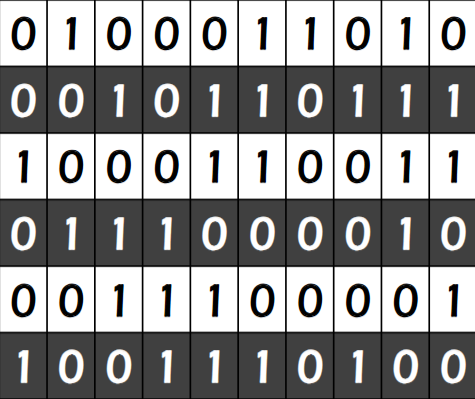
\includegraphics[width=0.75\linewidth]{images/init.png}
\end{figure}

\begin{itemize}
    \item Quần thể đầu tiên thường được khởi tạo một cách ngẫu nhiên với phân bố đồng nhất (uniformly random).
    \item[] $\triangleright$ Với mỗi bit của từng cá thể, phát sinh ngẫu nhiên một số $r \in [0..1]$.
    \item[] $\triangleright$ $r < 0.5 \rightarrow$ bit nhận giá trị 0.
    \item[] $\triangleright$ $r \ge 0.5 \rightarrow$ bit nhận giá trị 1.
    \item[] $\triangleright$ Cách tốt hơn?
    \item Có thể sử dụng thông tin về bài toán đang xét (nếu có) để khởi tạo quần thể với phân bố phù hợp hơn.
\end{itemize}

\subsection{Chọn lọc tỷ lệ (Proportional Selection)}

\begin{itemize}
    \item Phép chọn lọc: Lựa chọn (ngẫu nhiên) những cá thể (có độ thích nghi cao) làm cá thể cha mẹ (parents) để sinh ra những cá thể mới (cá thể con - offspring).
    \item Chọn lọc theo tỷ lệ: Xác suất một cá thể được chọn làm cá thể cha mẹ tỷ lệ thuận với độ thích nghi của cá thể đó.
    \item[] $\triangleright$ Những giải pháp tốt hơn được ưu tiên lựa chọn nhiều hơn để tạo ra những giải pháp mới.
\end{itemize}

\begin{itemize}
    \item $P$ là quần thể có $n$ cá thể.
    \item $P_i$ là cá thể thứ $i$ của $P$.
    \item $\text{fitness}[P_i]$ là độ thích nghi của $P_i$.
    \item Tổng giá trị thích nghi của $P$: $\Sigma^{n-1}_{i=0} \text{fitness}[P_i]$
    \item Xác suất cá thể $P_i$ được chọn $= $ tỷ lệ đóng góp của $P_i$ cho tổng giá trị thích nghi của $P$:
    $$ p_i^S = \frac{\text{fitness}[P_i]}{\sum_{t=0}^{n-1} \text{fitness}[P_t]} $$
\end{itemize}

Tạo ra tập lựa chọn $S$ (selection set) có $n$ cá thể cha mẹ từ quần thể $P$ gồm $n$ cá thể.
\begin{itemize}
    \item \textbf{Bước 1:} Tính xác suất lựa chọn $p_i^S$ của từng cá thể.
    \item \textbf{Bước 2:} Tính xác suất tích luỹ (cumulative probability) $p_i^{S,C}$ của từng cá thể: $p_i^{S,C} = \sum_{j=0}^{i} p_j^S$
    \item \textbf{Bước 3:} Phát sinh ngẫu nhiên 1 số thực $r \in [0..1)$.
    \item \textbf{Bước 4:} Chọn cá thể $P_i$ sao cho $p_{i-1}^{S,C} \le r < p_i^{S,C}$ với $i \in \{0,1, \ldots, n-1\}$ và $p_{-1}^{S,C} = 0$.
    Lặp lại bước 3 - 4 tới khi chọn đủ $n$ cá thể.
\end{itemize}

\subsection*{Ví dụ:} % Tiêu đề phụ không đánh số cho ví dụ
\begin{itemize}
    \item Một quần thể có 5 cá thể với độ thích nghi là $(1, 4, 3, 1, 1)$.
    \item Tỷ lệ đóng góp của từng cá thể vào tổng giá trị thích nghi là $(0.1, 0.4, 0.3, 0.1, 0.1) \rightarrow$ xác suất được chọn $p_i^S$ của từng cá thể.
    \item Xác suất tích luỹ $p_i^{S,C}$ của từng cá thể là $(0.1, 0.5, 0.8, 0.9, 1.0)$.
\end{itemize}

\begin{figure}[H]
    \centering
    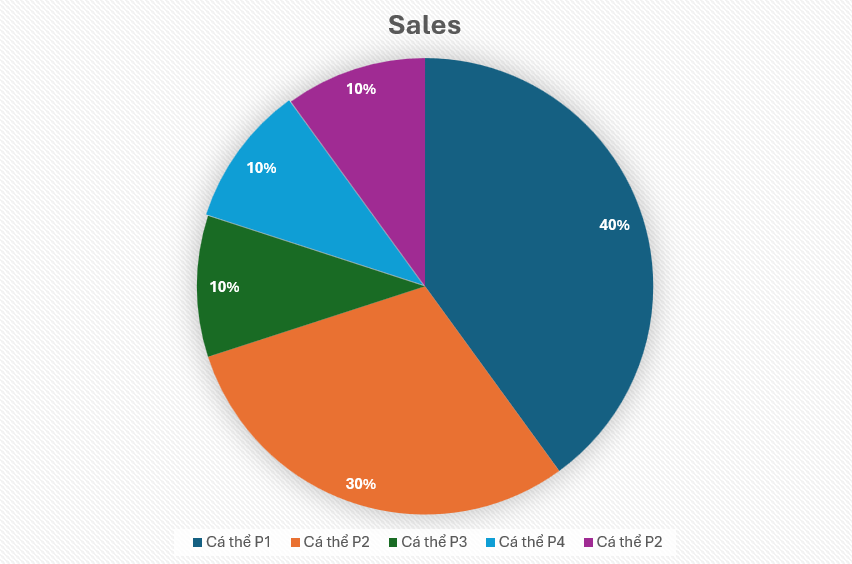
\includegraphics[width=0.7\textwidth]{images/pie_chart.png} 
\end{figure}

% Nội dung từ ảnh mới nhất (image_9025f1.png)
\begin{center}
    \textbf{XÁC SUẤT LỰA CHỌN}
\end{center}

\begin{figure}[H]
    \centering
    \begin{minipage}[c]{0.45\textwidth} % Dùng minipage để đặt hình ảnh và text cạnh nhau
        \centering
        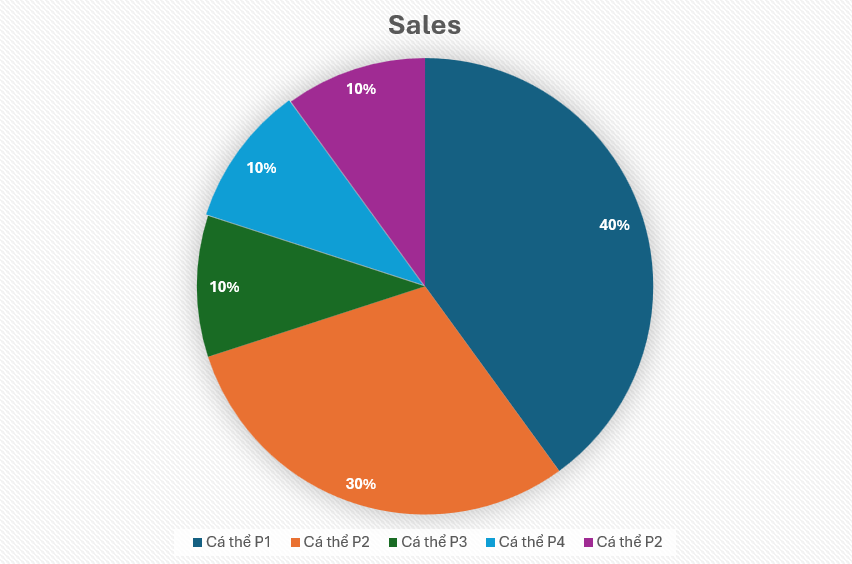
\includegraphics[width=\linewidth]{images/pie_chart.png} % Thay bằng tên file biểu đồ tròn của bạn nếu có
        % Nếu đây là cùng một hình với cái trên, bạn có thể dùng lại
    \end{minipage}
    \begin{minipage}[c]{0.45\textwidth}
        \textbf{Ví dụ:}
        \begin{itemize}
            \item $r = 0.37 \rightarrow$ lựa chọn cá thể $P_1$
            \item $r = 0.07 \rightarrow$ lựa chọn cá thể $P_0$
            \item $r = 0.39 \rightarrow$ lựa chọn cá thể $P_1$
            \item $r = 0.72 \rightarrow$ lựa chọn cá thể $P_2$
            \item $r = 0.34 \rightarrow$ lựa chọn cá thể $P_1$
        \end{itemize}
    \end{minipage}
\end{figure}

\begin{figure}[H]
    \centering
    \begin{minipage}[c]{0.45\textwidth} % Dùng minipage để đặt hình ảnh và text cạnh nhau
        \centering
        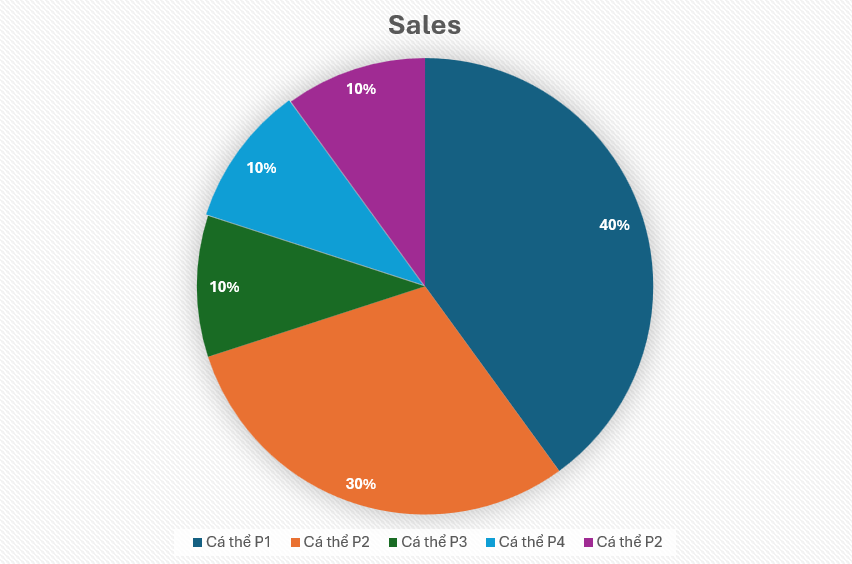
\includegraphics[width=\linewidth]{images/pie_chart.png} % Thay bằng tên file biểu đồ tròn của bạn nếu có
    \end{minipage}
    \begin{minipage}[c]{0.45\textwidth}
        \textbf{Ví dụ:}
        \begin{itemize}
            \item $r = \dots \rightarrow$ lựa chọn $\dots$
            \item $r = \dots \rightarrow$ lựa chọn $\dots$
            \item $r = \dots \rightarrow$ lựa chọn $\dots$
            \item $r = \dots \rightarrow$ lựa chọn $\dots$
            \item $r = \dots \rightarrow$ lựa chọn $\dots$
        \end{itemize}
        \begin{itemize}
            \item[] $\triangleright$ Proportional selection còn được gọi là Roulette wheel selection.
        \end{itemize}
    \end{minipage}
\end{figure}

\subsection{Các phép biến đổi (Variation)}

\begin{itemize}
    \item Phép biến đổi: được thực hiện trên tập lựa chọn $S$ (selection set) nhằm tạo ra các cá thể mới (offspring) từ các cá thể cha mẹ (parents).
    \item Thuật giải di truyền GA có 2 phép biến đổi chính:
    \begin{itemize}
        \item[] $\triangleright$ Lai ghép (crossover), còn được gọi là Tái tổ hợp (recombination).
        \item[] $\triangleright$ Đột biến (mutation).
    \end{itemize}
\end{itemize}

\subsection{Phép biến đổi - Lai ghép}

Phép lai ghép: Tạo ra cá thể mới bằng cách kết hợp kiểu gen của những cá thể (có độ thích nghi cao) trong quần thể.

\begin{table}[h!]
    \centering
    \begin{tabular}{|c|c|c|} % Đã thay 'l' thành 'c' cho cột thứ nhất và thứ ba
        \hline
        \textbf{Cá thể cha mẹ (Parents)} & \textbf{Phép lai (Crossover)} & \textbf{Cá thể con (Offspring)} \\
        \hline
        000000000000 & Lai một điểm & 0000\textbf{11111111} \\
        \textbf{111111111111} & (One-point crossover - 1X) & \textbf{1111}00000000 \\
        \hline
        000000000000 & Lai hai điểm & 000\textbf{111111}000 \\
        \textbf{111111111111} & (Two-point crossover - 2X) & \textbf{111}000000\textbf{111} \\
        \hline
        000000000000 & Lai đồng nhất & \textbf{1}0\textbf{11}000\textbf{1}0\textbf{11}0 \\
        \textbf{111111111111} & (Uniform crossover - UX) & 0\textbf{1}00\textbf{111}0\textbf{1}00\textbf{1} \\
        \hline
    \end{tabular}
    %\caption{Các loại lai ghép cơ bản} % Bạn có thể thêm chú thích nếu muốn
    \label{tab:crossover_types}
\end{table}

\subsubsection{Lai một điểm}
\begin{figure}[H]
    \centering
    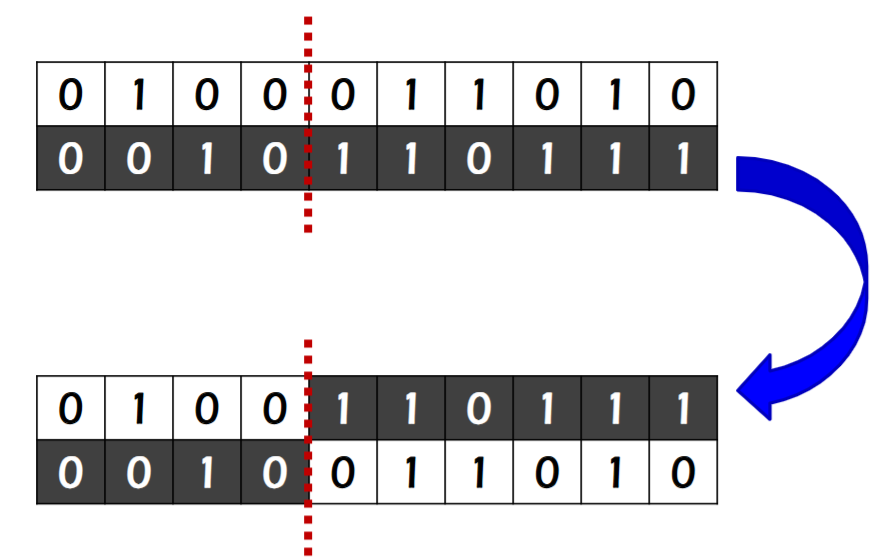
\includegraphics[width=0.75\linewidth]{images/laimotdiem1.png}
\end{figure}

\begin{figure}[H]
    \centering
    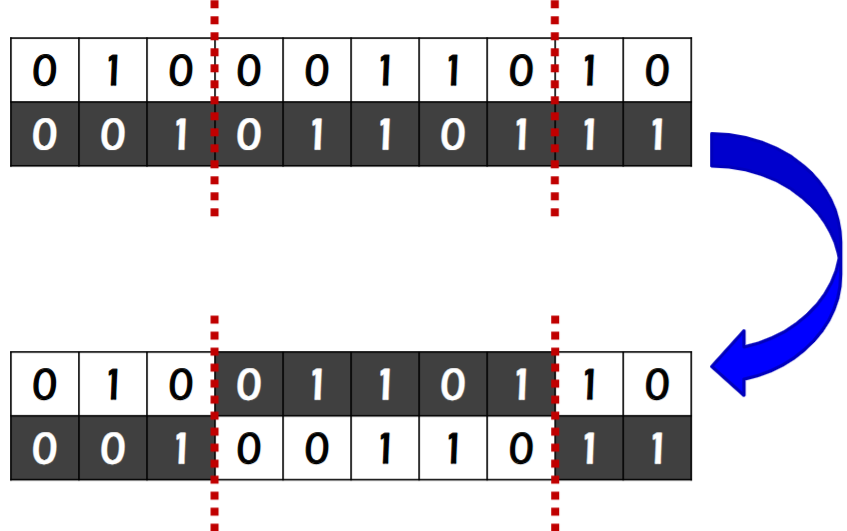
\includegraphics[width=0.75\linewidth]{images/laimotdiem2.png}
\end{figure}

\subsubsection{Lai đồng nhất}
\begin{figure}[H]
    \centering
    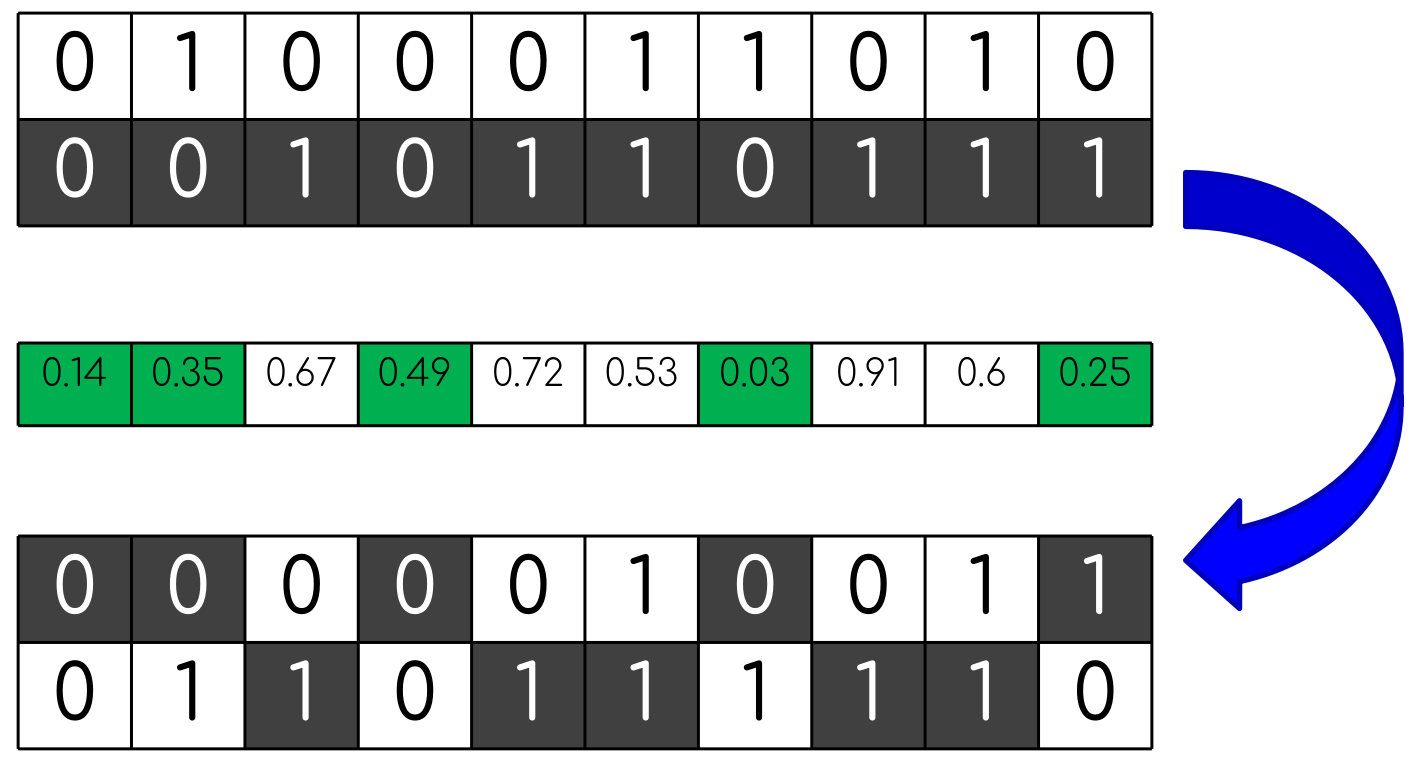
\includegraphics[width=0.75\linewidth]{images/laidongnhat.png}
\end{figure}

\begin{itemize}
    \item Lựa chọn xác suất lai $p_c$.
    \item Ghép cặp các cá thể trong tập lựa chọn $S$.
    \item Với mỗi cặp đôi cá thể cha mẹ, phát sinh ngẫu nhiên 1 số thực $r \in [0..1)$.
    \item[] $\triangleright$ Nếu $r < p_c$, tiến hành phép lai tạo ra 2 cá thể con mới.
    \item[] $\triangleright$ Ngược lại, 2 cá thể con là sao chép (clone) của 2 cá thể cha mẹ.
\end{itemize}

\subsection{Phép biến đổi – Đột biến} % Sử dụng \subsubsection* để không đánh số
\begin{itemize}
    \item Phép đột biến: Tạo ra cá thể mới bằng cách phát sinh những biến đổi ngẫu nhiên trên kiểu gen của các cá thể trong quần thể.
    \item Lựa chọn xác suất đột biến $p_m$ (thường nhỏ).
    \item Với mỗi bit của từng cá thể, phát sinh ngẫu nhiên 1 số thực $r \in [0..1)$.
    \item[] $\triangleright$ Nếu $r < p_m$, đảo ngược giá trị của bit ($0 \rightarrow 1$ hoặc $1 \rightarrow 0$).
    \item[] $\triangleright$ Ngược lại, giữ nguyên giá trị của bit.
\end{itemize}

\subsubsection{Đột biến}
\begin{figure}[H]
    \centering
    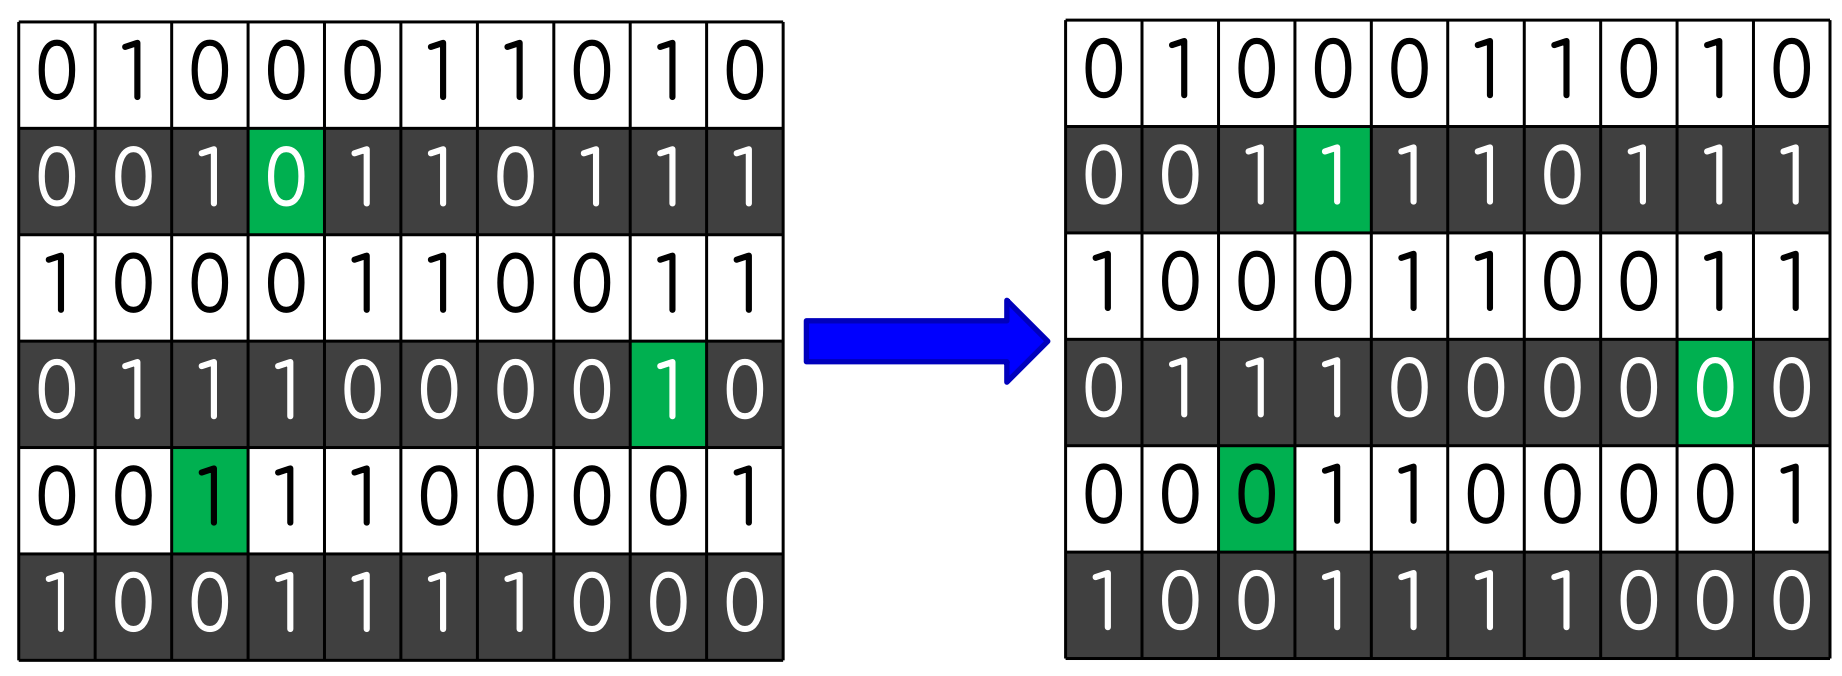
\includegraphics[width=0.75\linewidth]{images/dotbien.png}
\end{figure}

\subsection{Điều kiện dừng (Termination)}

\begin{itemize}
    \item Sử dụng hết tài nguyên tính toán.
    \begin{itemize}
        \item[] $\triangleright$ Thời gian.
        \item[] $\triangleright$ Số lần gọi hàm lượng giá (evaluation function calls).
    \end{itemize}
    \item Quần thể không còn độ đa dạng (diversity).
    \begin{itemize}
        \item[] $\triangleright$ Các cá thể trong quần thể gần giống nhau về kiểu gen.
        \item[] $\triangleright$ Các cá thể trong quần thể có độ thích nghi gần giống nhau.
    \end{itemize}
    \item Đạt được độ thích nghi mong muốn.
    \item Tìm được một giải pháp chấp nhận được cho bài toán.
\end{itemize}

\subsection{Flowchart}
\begin{figure}[H]
    \centering
    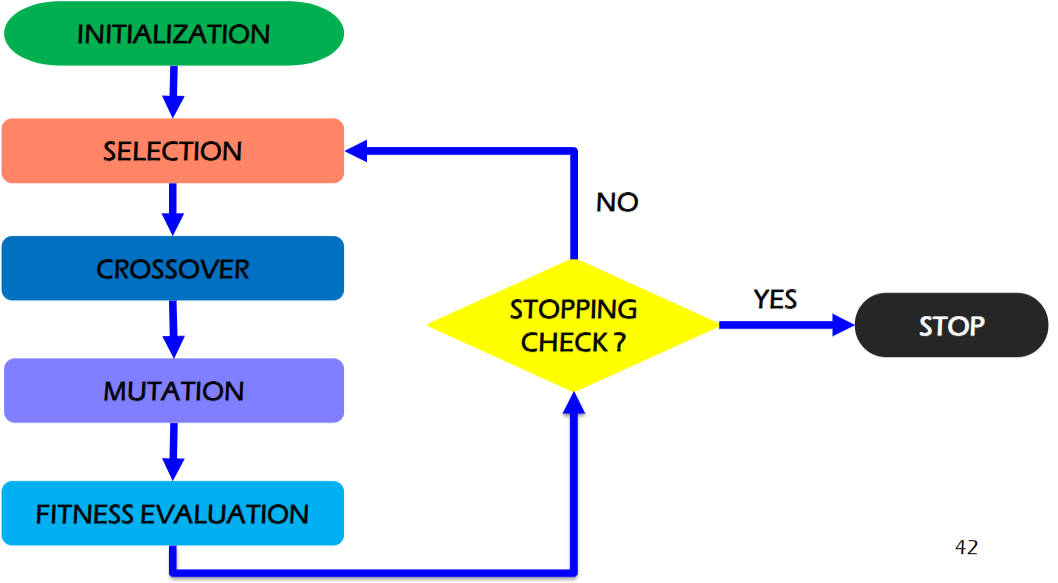
\includegraphics[width=0.75\linewidth]{images/flowchart.png}
\end{figure}

\subsection{Ví dụ}

\subsubsection{VD1} Độ thích nghi trung bình là 177.0
\begin{table}[H]
    \centering
    \begin{tabular}{|c|c|} % Thay p{3cm} và p{2cm} bằng c
    \hline
    \textbf{P0} & \textbf{Fitness} \\
    \hline
    10010 & 324 \\
    01100 & 144 \\
    01001 & 81 \\
    10100 & 400 \\
    01000 & 64 \\
    00111 & 49 \\
    \hline
    \end{tabular}
\end{table}

\subsubsection{VD2} Độ thích nghi trung bình của quần thể P1 là 318.8
\begin{table}[H]
    \centering
    \begin{tabular}{|c|c|c|c|c|c|}
    \hline
    \textbf{P0} & \textbf{Fitness} & \textbf{Selection} & \textbf{Crossover} & \textbf{Mutation} & \textbf{Fitness} \\
    \hline
    10010 & 324 & 10010 & 10 $|$ 010 & 10100 & 400 \\
    01100 & 144 & 10100 & 10 $|$ 100 & 10010 & 324 \\
    01001 & 81 & 01000 & 010 $|$ 00 & 01010 & 100 \\
    10100 & 400 & 10010 & 100 $|$ 10 & 1000\textcolor{red}{\textbf{1}} & 289 \\ % Chú ý số 1 in đậm
    01000 & 64 & 01100 & 0 $|$ 1100 & 00100 & 16 \\
    00111 & 49 & 10100 & 1 $|$ 0100 & 11100 & 784 \\
    \hline
    \end{tabular}
    % \caption{Bảng ví dụ minh họa quá trình tiến hóa} % Bạn có thể thêm caption nếu muốn
    % \label{tab:evolution_example}
\end{table}

\subsubsection{VD3} Độ thích nghi trung bình của quần thể P2 là 426.3
\begin{table}[H]
    \centering
    \begin{tabular}{|c|c|c|c|c|c|}
    \hline
    \textbf{P1} & \textbf{Fitness} & \textbf{Selection} & \textbf{Crossover} & \textbf{Mutation} & \textbf{Fitness} \\
    \hline
    10100 & 400 & 11100 & 111 $|$ 00 & 11110 & 900 \\
    10010 & 324 & 10010 & 100 $|$ 10 & 10000 & 256 \\
    01010 & 100 & 10001 & 10 $|$ 001 & \textcolor{red}{\textbf{0}}0100 & 16 \\ % Chú ý số 0 in đậm
    10001 & 289 & 10100 & 10 $|$ 100 & 10001 & 289 \\
    00100 & 16 & 10001 & 100 $|$ 01 & 10000 & 256 \\
    11100 & 784 & 11100 & 111 $|$ 00 & 11101 & 841 \\
    \hline
    \end{tabular}
    % \caption{Bảng ví dụ minh họa quá trình tiến hóa tiếp theo} % Bạn có thể thêm caption nếu muốn
    % \label{tab:evolution_example_p2}
\end{table}

\subsubsection{VD4} Độ thích nghi trung bình của quần thể P3 là 654.5
\begin{table}[H]
    \centering
    \begin{tabular}{|c|c|c|c|c|c|}
    \hline
    \textbf{P2} & \textbf{Fitness} & \textbf{Selection} & \textbf{Crossover} & \textbf{Mutation} & \textbf{Fitness} \\
    \hline
    11110 & 900 & 11110 & 111 $|$ 10 & 11101 & 841 \\
    10000 & 256 & 10001 & 100 $|$ 01 & 10010 & 324 \\
    00100 & 16 & 11101 & 11 $|$ 101 & 11000 & 576 \\
    10001 & 289 & 10000 & 10 $|$ 000 & 10101 & 441 \\
    10000 & 256 & 11110 & 1111 $|$ 0 & 11111 & 961 \\
    11101 & 841 & 11101 & 1110 $|$ 1 & 11100 & 784 \\
    \hline
    \end{tabular}
    % \caption{Bảng ví dụ minh họa quá trình tiến hóa tiếp theo (P2)} % Optional caption
    % \label{tab:evolution_example_p3}
\end{table}

\subsubsection{VD5} Độ thích nghi trung bình của quần thể P4 là 862.0
\begin{table}[H]
    \centering
    \begin{tabular}{|c|c|c|c|c|c|}
    \hline
    \textbf{P3} & \textbf{Fitness} & \textbf{Selection} & \textbf{Crossover} & \textbf{Mutation} & \textbf{Fitness} \\
    \hline
    11101 & 841 & 11101 & 11 $|$ 101 & 11111 & 961 \\
    10010 & 324 & 11111 & 11 $|$ 111 & 11101 & 841 \\
    11000 & 576 & 11100 & 1 $|$ 1100 & 11101 & 841 \\
    10101 & 441 & 11101 & 1 $|$ 1101 & 11100 & 784 \\
    11111 & 961 & 11111 & 111 $|$ 11 & 11100 & 784 \\
    11100 & 784 & 11000 & 110 $|$    00 & 11\textcolor{red}{\textbf{1}}11 & 961 \\ % Chú ý số 1 in đậm
    \hline
    \end{tabular}
    % \caption{Bảng ví dụ minh họa quá trình tiến hóa tiếp theo (P3)} % Chú thích tùy chọn
    % \label{tab:evolution_example_p4}
\end{table}
\chapter{Genetic Algorithm (POPOP)}
\section{Genetic Algorithm}
\subsection{Chọn lọc tỷ lệ (Proportional Selection)}
\begin{itemize}
    \item $P$ là quần thể có $n$ cá thể
    \item $P_i$ là cá thể thứ $i$ của $P$
    \item $\operatorname{fitness}(P_i)$ là độ thích nghi của $P_i$
    \item Tổng giá trị thích nghi của $P$: $\sum_{i=0}^{n-1} \operatorname{fitness}(P_i)$
    \item Xác suất cá thể $P_i$ được chọn $= $ tỷ lệ đóng góp của $P_i$ cho tổng giá trị thích nghi của $P$:
    \begin{equation*}
        p_i^S=\frac{\operatorname{fitness}(P_i)}{\sum_{i=0}^{n-1} \operatorname{fitness}(P_i)}
    \end{equation*}
\end{itemize}
\begin{itemize}
    \item Một quần thể có 5 cái thể với độ thích nghi là $(1, 4, 3, 1, 1)$.
    \item Tỷ lệ đóng góp của từng cá thể vào tổng giá trị thích nghi là $(0.1, 0.4, 0.3, 0.1, 0.1)$ $\to$ xác suất được chọn $p^S_i$ của từng cá thể.
\end{itemize}
\begin{figure}[H]
    \centering
    \begin{minipage}[c]{0.45\textwidth}
        \centering
        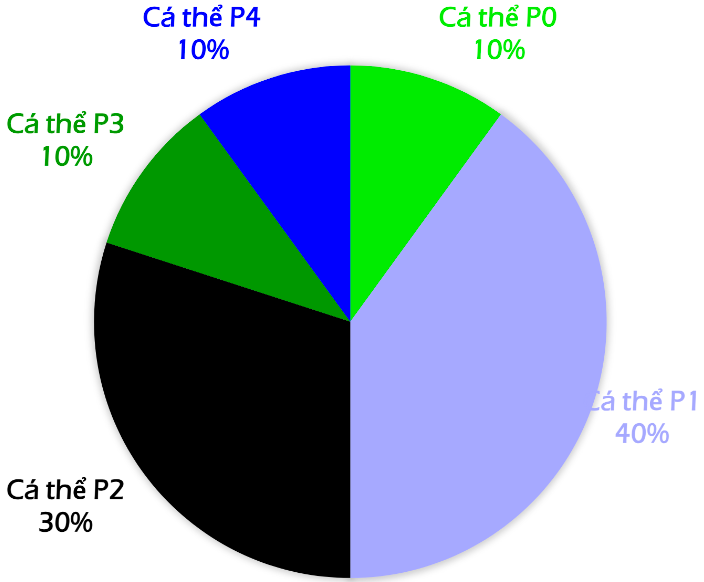
\includegraphics[width=0.7\linewidth]{images/proportional_selection_pie_2.png} 
    \end{minipage}%
    \hfill
    \begin{minipage}[c]{0.45\textwidth}
        \textbf{Ví dụ:}
        \begin{itemize}
            \item $r = 0.37 \rightarrow$ lựa chọn cá thể $P_1$
            \item $r = 0.07 \rightarrow$ lựa chọn cá thể $P_0$
            \item $r = 0.39 \rightarrow$ lựa chọn cá thể $P_1$
            \item $r = 0.72 \rightarrow$ lựa chọn cá thể $P_2$
            \item $r = 0.34 \rightarrow$ lựa chọn cá thể $P_1$
        \end{itemize}
    \end{minipage}
    \caption{Minh họa chọn lọc tỷ lệ và ví dụ quay roulette.}
    \label{fig:proportional_selection_example}
\end{figure}
\begin{itemize}
    \item Khuyết điểm của Proportional Selection (chọn lọc tỷ lệ) là gì? (Câu trả lời phía dưới được tạo sinh bởi Gemini Pro 2.5)
    \begin{itemize}
        \item \textbf{Hội tụ sớm (Premature Convergence)}: Các cá thể có độ thích nghi vượt trội (super-fit) có thể nhanh chóng chiếm đa số trong quần thể, làm giảm sự đa dạng di truyền và khiến thuật toán bị mắc kẹt ở mức tối ưu cục bộ thay vì tìm ra giải pháp tối ưu toàn cục.
        \item \textbf{Mất mát các cá thể tốt (nhưng không vượt trội)}: Khi có sự chênh lệch lớn về độ thích nghi, các cá thể tốt nhưng không phải tốt nhất sẽ có rất ít cơ hội được chọn, dẫn đến nguy cơ bị loại bỏ khỏi quần thể.
        \item \textbf{Nhạy cảm với sự phân bố độ thích nghi}: Hiệu suất của phương pháp phụ thuộc nhiều vào sự phân bố giá trị thích nghi trong quần thể. Nếu các giá trị này gần bằng nhau, việc chọn lọc sẽ gần như ngẫu nhiên.
        \item \textbf{Vấn đề với giá trị thích nghi âm}: Phương pháp này không thể áp dụng trực tiếp cho các bài toán mà giá trị độ thích nghi có thể là số âm.
        \item \textbf{Tỷ lệ chọn lọc không ổn định}: Tỷ lệ chọn lọc cho một cá thể không chỉ phụ thuộc vào độ thích nghi của chính nó mà còn phụ thuộc vào độ thích nghi của tất cả các cá thể khác trong quần thể, gây ra sự thiếu ổn định.
    \end{itemize}
\end{itemize}
\subsection{Tournament Selection}
\begin{itemize}
    \item Tournament Selection (Chọn lọc cạnh tranh/Chọn lọc giao đấu): Mỗi lần lấy ngẫu nhiên $s$ cá thể từ quần thể và lựa chọn cá thể có độ thích nghi tốt nhất trong $s$ cá thể này.
    \item $s$ còn được gọi là \textit{tournament size}.
    \item Ví dụ: $\mathbf{x}$ là chuỗi nhị phân có $l$ bit. Tìm giá trị của $\mathbf{x}$ để hàm \texttt{OneMax} đạt giá trị tối đa. \begin{equation*}
        f_{\texttt{OneMax}}(x)=\sum_{i=1}^{l}{x_i}
    \end{equation*}
\end{itemize}
\begin{figure}[H]
    \centering
    \begin{minipage}[c]{0.45\textwidth}
        \centering
        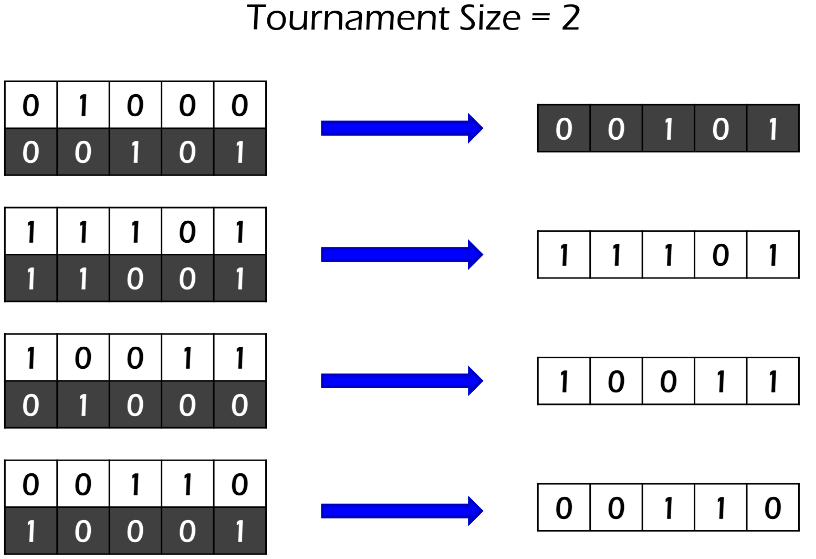
\includegraphics[width=\linewidth]{images/tournament_selection_ex1.png}
    \end{minipage}\hfill
    \begin{minipage}[c]{0.45\textwidth}
        \centering
        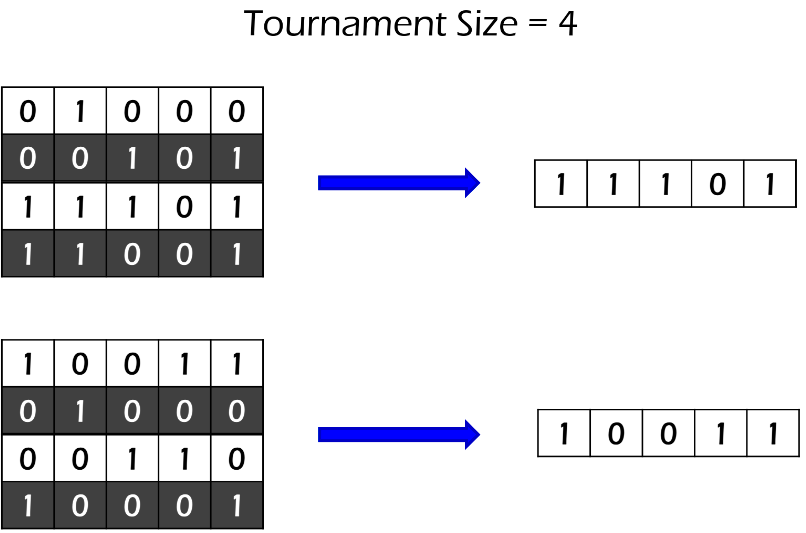
\includegraphics[width=\linewidth]{images/tournament_selection_ex2.png}
    \end{minipage}
    \caption{Ví dụ về chọn lọc cạnh tranh}
    \label{fig:tournament_selection_ex}
\end{figure}
\begin{figure}[H]
    \centering
    \begin{minipage}[c]{0.45\textwidth}
        \centering
        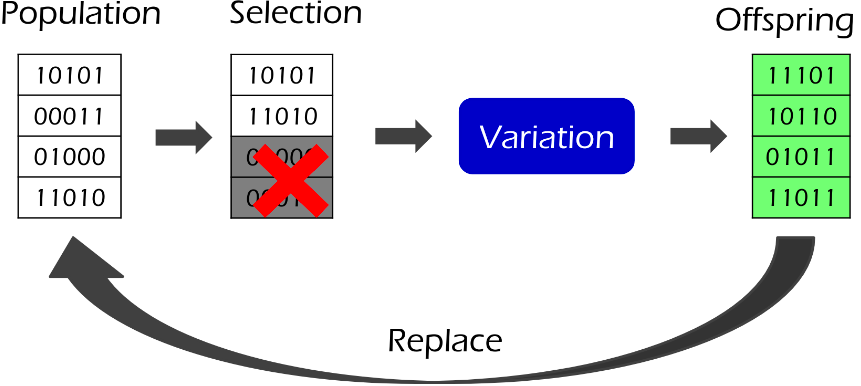
\includegraphics[width=\linewidth]{images/without_POPOP.png}
        \subcaption{Bản cài đặt GA không có POPOP}
        \label{fig:without_POPOP}
    \end{minipage}\hfill
    \begin{minipage}[c]{0.45\textwidth}
        \centering
        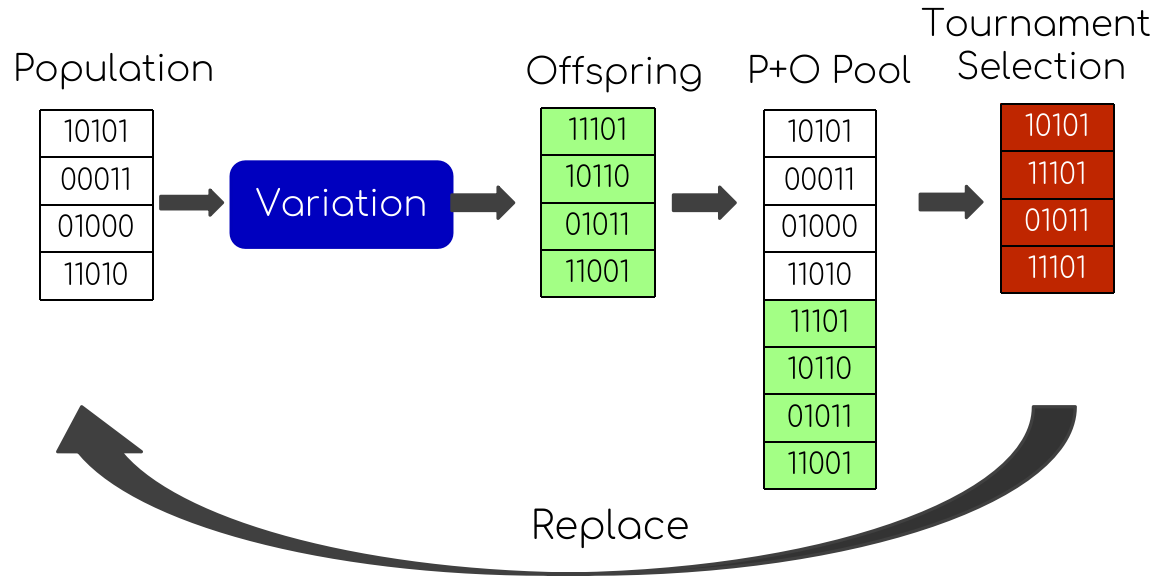
\includegraphics[width=\linewidth]{images/POPOP.png}
        \subcaption{Bản cài đặt GA có POPOP}
        \label{fig:POPOP}
    \end{minipage}
    \caption{So sánh GA có và không có POPOP.}
    \label{fig:ga_popop_comparison}
\end{figure}
\begin{itemize}
    \item Bản cài đặt không có POPOP (thể hiện ở hình~\ref{fig:without_POPOP}): có nhược điểm: có nguy cơ đánh mất các cá thể tốt nhất (elitism) đã tìm được, dẫn đến sự hội tụ không ổn định và thậm chí làm giảm chất lượng của quần thể qua các thế hệ.
    \item Bản cài đặt có sử dụng POPOP (thể hiện ở hình~\ref{fig:POPOP}) đảm bảo rằng giải pháp tốt nhất được tìm thấy sẽ không bao giờ bị mất đi. Chất lượng của quần thể sẽ không bao giờ suy giảm qua các thế hệ (monotonically non-decreasing fitness), giúp thuật toán hội tụ nhanh và ổn định hơn tới một giải pháp tốt.
\end{itemize}
\chapter{Simple Genetic Algorithm (sGA)}
\begin{figure}[H]
    \centering
    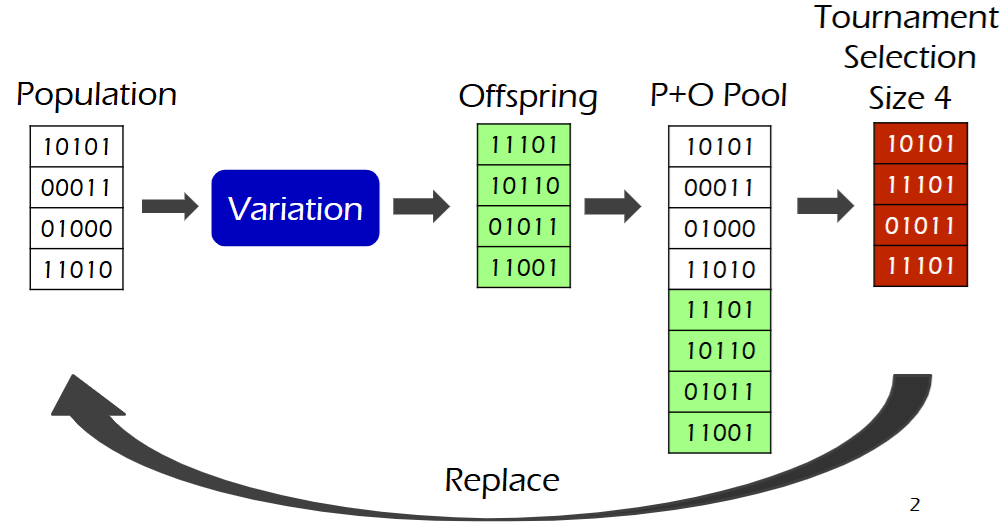
\includegraphics[width=0.75\linewidth]{images/GA-3_1.png}
\end{figure}

\begin{itemize}
    \item Tối thiểu hoá $f(x_0, x_1) = (x_0 - 0.5)^2 + (x_1 - 0.5)^2$
    \\ $x_0, x_1 \in [0,1] \subset \mathbb{R}$

\end{itemize}

\begin{table}[h!]
    \centering
    \begin{tabular}{|c|c|}
    \hline
    \textbf{$x_0$} & \textbf{$x_1$} \\
    \hline
    0.25 & 0.80 \\
    0.40 & 0.97 \\
    0.12 & 0.34 \\
    0.67 & 0.72 \\
    0.55 & 0.81 \\
    0.52 & 0.04 \\
    0.85 & 0.23 \\
    0.76 & 0.65 \\
    \hline
    \end{tabular}
\end{table}

sGA có thể giải quyết các bài toán với các \textcolor{red}{biến số thực} không?

\section{sGA – Simple Binary Encoding}

Một chuỗi nhị phân $(a_i)$ với $q$ bit
\[
(a_i), \quad a_i \in \{0,1\}, \quad i = 0,1, \dots, q-1
\]
có thể biểu diễn một biến số thực $x \in [b_L, b_U]$, và giá trị của $x$ là
\[
x = b_L + \frac{b_U - b_L}{2^q - 1} \sum_{i=0}^{q-1} a_i 2^i
\]

Ví dụ: Sử dụng $q=3$ bit để biểu diễn một biến số thực $x \in [0,1]$

\begin{center}
\begin{tikzpicture}[xscale=5]
  % Tick marks and labels
  \foreach \x/\bin/\label in {
    0/000/0.00,
    1/001/0.14,
    2/010/0.28,
    3/011/0.43,
    4/100/0.57,
    5/101/0.71,
    6/110/0.86,
    7/111/1.00
  } {
    \draw[thick] (\x*0.14,0.1) -- (\x*0.14,-0.1);
    \node[above] at (\x*0.14,0.1) {\label};
    \node[below] at (\x*0.14,-0.1) {\bin};
  }
  % Draw line
  \draw[thick] (0,0) -- (0.14*7,0);
\end{tikzpicture}
\end{center}

Có vấn đề gì với cách biểu diễn nhị phân này?

\begin{itemize}
    \item Thuật toán phải xử lý nhiều biến hơn (số biến tăng q lần).
    \item Các giá trị gần nhau có thể có cách biểu diễn khác hẳn nhau. Ví dụ: 0.43 (011) và 0.57 (100).
    \item ...
\end{itemize}

\chapter{DE (Differential Evolution)}

\section{DE - Giới thiệu}
\begin{itemize}
    \item Differential Evolution (DE) được đề xuất bởi Storn và Price vào năm 1995.
    \item Ý tưởng chính: Phép biến đổi được thực hiện bằng cách cộng vector khác biệt giữa hai cá thể được chọn ngẫu nhiên vào một cá thể thứ ba được chọn ngẫu nhiên khác.
\end{itemize}

\section{DE – Các kí hiệu}

\begin{itemize}
    \item Quần thể $P_{X,g}$ ở thế hệ $g$ có chứa $N$ vector $x_{i,g}$
    $$ P_{X,g} = (x_{i,g}), i = 0,1, \dots, N-1, g = 0,1, \dots, g_{\max} $$
    $$ x_{i,g} = (x_{i,j,g}), j = 0,1, \dots, D-1 $$
    $$ x_{i,j,g} \in [b_{j,L}, b_{j,U}] \subset \mathbb{R} $$
    \item N: kích thước quần thể.
    \item D: số biến – số tham số.
    \item $g_{\max}$: số thế hệ tối đa.
    \item $[b_{j,L}, b_{j,U}]$: miền giá trị của biến thứ $j$
\end{itemize}

\section{DE – Khởi tạo quần thể}

$$ g = 0 $$
$$ P_{X,0} = (x_{i,0}) $$
$$ x_{i,j,0} \in \text{rand}(0,1) \times (b_{j,U} - b_{j,L}) + b_{j,L} $$
$$ 0 \le \text{rand}(0,1) \le 1 $$

\section{DE – Tạo ra vector đột biến}

Quần thể đột biến (mutant population) $P_{V,g}$ chứa N vector đột biến (mutant vector) $v_{i,g}$
$$ P_{V,g} = (v_{i,g}), i = 0,1, \dots, N-1, g = 0,1, \dots, g_{\max} $$
$$ v_{i,g} = (v_{i,j,g}), j = 0,1, \dots, D-1 $$
F: hệ số scale, thường thì F $\in$ (0,1) \\
Với mỗi vector $v_{i,g}$:
\begin{itemize}
    \item Chọn ngẫu nhiên $r_0, r_1, r_2$ từ $\{0,1, \dots, N-1\} \setminus \{i\}$
    \item $x_{r_0,g}, x_{r_1,g}, x_{r_2,g} \in P_{X,g}$
\end{itemize}

$$ v_{i,g} = x_{r_0,g} + F \times (x_{r_1,g} - x_{r_2,g}) $$

Xét từng vector $x_{i,g}$

\begin{figure}[H]
    \centering
    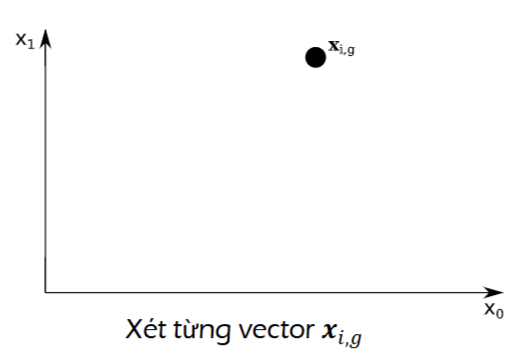
\includegraphics[width=0.75\linewidth]{images/GA-3_2.png}
\end{figure}

\begin{figure}[H]
    \centering
    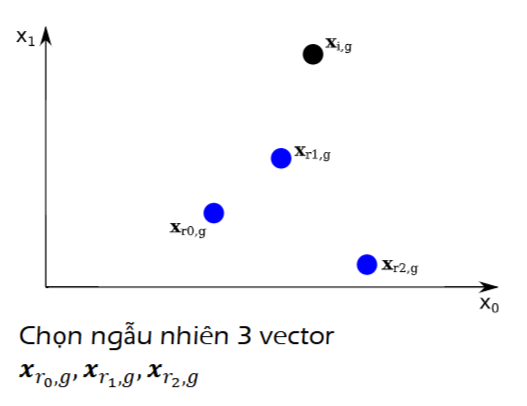
\includegraphics[width=0.75\linewidth]{images/GA-3_3.png}
\end{figure}

\begin{figure}[H]
    \centering
    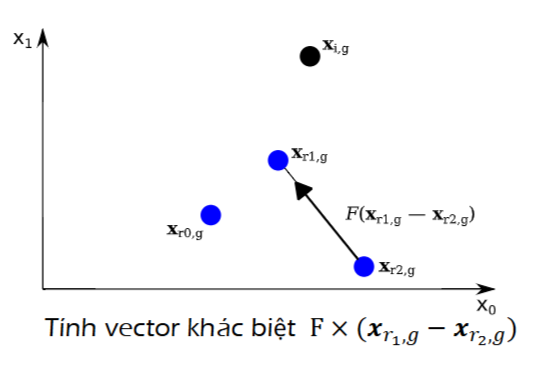
\includegraphics[width=0.75\linewidth]{images/GA-3_4.png}
\end{figure}

\begin{figure}[H]
    \centering
    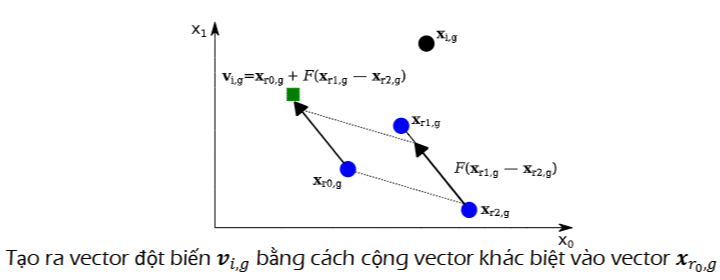
\includegraphics[width=1\linewidth]{images/GA-3_5.png}
\end{figure}

\section{DE – Lai ghép}

Quần thể thử nghiệm (trial population) $P_{U,g}$ chứa N vector thử nghiệm (trial vector) $u_{i,g}$
$$ P_{U,g} = (u_{i,g}), i = 0,1, \dots, N-1, g = 0,1, \dots, g_{\max} $$
$$ u_{i,g} = (u_{j,i,g}), j = 0,1, \dots, D-1 $$
Cr: Xác suất lai ghép. Với mỗi vector $u_{i,g}$:
\begin{itemize}
    \item $j_{\text{rand}}$: Một chỉ số ngẫu nhiên được chọn từ $\{0,1, \dots, D-1\}$
    \item Vector đích (target vector) $x_{i,g} \in P_{X,g}$
\end{itemize}

$$ u_{j,i,g} = \begin{cases}
v_{j,i,g} & \text{nếu rand}_j(0,1) \le \text{Cr hoặc } j = j_{\text{rand}} \\
x_{j,i,g} & \text{trong trường hợp ngược lại}
\end{cases} $$

\begin{figure}[H]
    \centering
    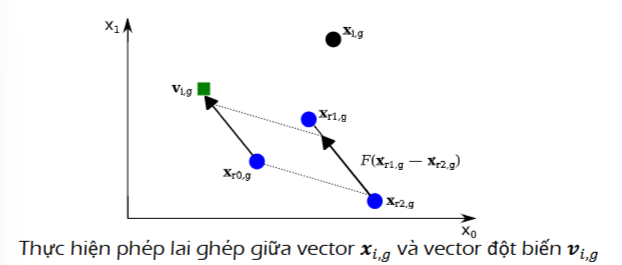
\includegraphics[width=1\linewidth]{images/GA-3_6.png}
\end{figure}

\begin{figure}[H]
    \centering
    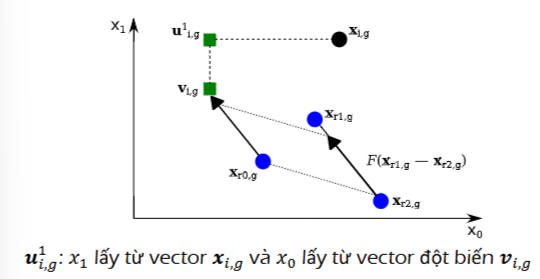
\includegraphics[width=1\linewidth]{images/GA-3_7.png}
\end{figure}

\begin{figure}[H]
    \centering
    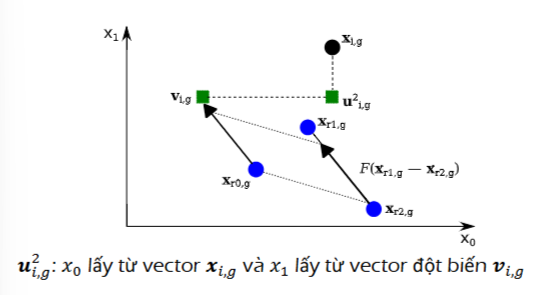
\includegraphics[width=1\linewidth]{images/GA-3_8.png}
\end{figure}

\begin{figure}[H]
    \centering
    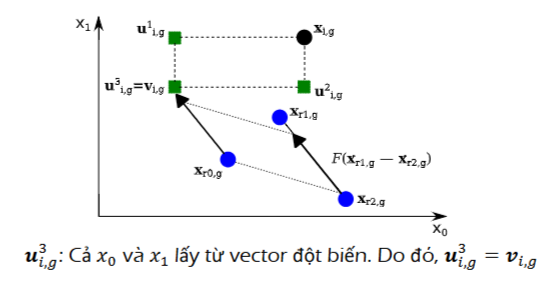
\includegraphics[width=1\linewidth]{images/GA-3_9.png}
\end{figure}

\section{DE – Chọn lọc}

Quần thể trong thế hệ tiếp theo $P_{X,g+1}$ chứa N vector $x_{i,g+1}$
$$ P_{X,g+1} = (x_{i,g+1}), i = 0,1, \dots, N-1, g = 0,1, \dots, g_{\max} $$
$$ x_{i,g+1} = \begin{cases}
u_{i,g} & \text{nếu } f(u_{i,g}) \text{ tốt hơn } f(x_{i,g}) \\
x_{i,g} & \text{trong trường hợp ngược lại}
\end{cases} $$

\section{DE - Ví dụ}
\begin{figure}[H]
    \centering
    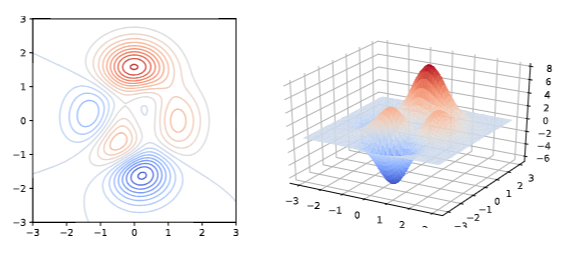
\includegraphics[width=0.75\linewidth]{images/GA-3_10.png}
\end{figure}

\begin{figure}[H]
    \centering
    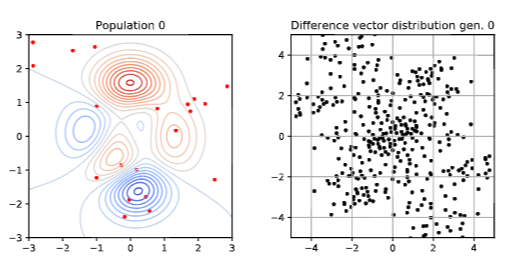
\includegraphics[width=0.75\linewidth]{images/GA-3_11.png}
\end{figure}

\begin{figure}[H]
    \centering
    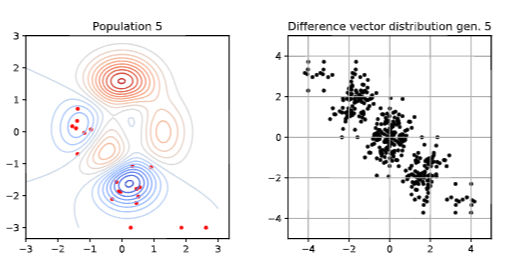
\includegraphics[width=0.75\linewidth]{images/GA-3_12.png}
\end{figure}

\begin{figure}[H]
    \centering
    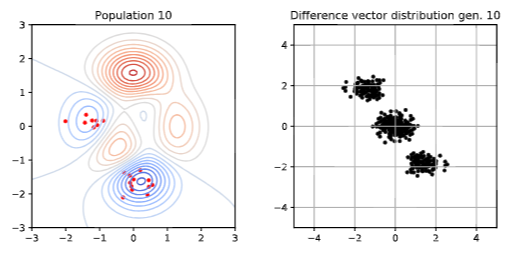
\includegraphics[width=0.75\linewidth]{images/GA-3_13.png}
\end{figure}

\begin{figure}[H]
    \centering
    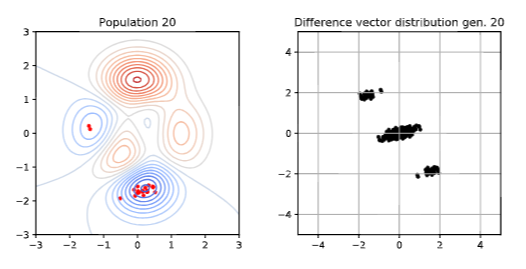
\includegraphics[width=0.75\linewidth]{images/GA-3_14.png}
\end{figure}

\begin{figure}[H]
    \centering
    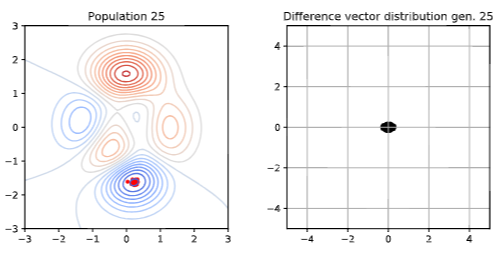
\includegraphics[width=0.75\linewidth]{images/GA-3_15.png}
\end{figure}

\begin{figure}[H]
    \centering
    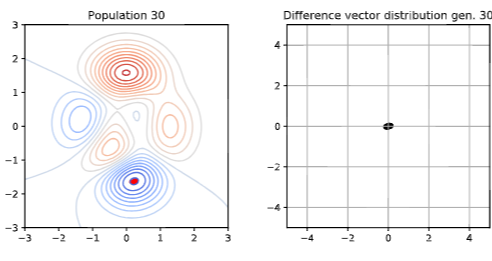
\includegraphics[width=0.75\linewidth]{images/GA-3_16.png}
\end{figure}

\section{DE – Các tham số điều khiển}

Hiệu suất của DE bị ảnh hưởng bởi các tham số điều khiển:
\begin{itemize}
    \item Kích thước quần thể
    \item Cách các vector $x_{r_0,g}, x_{r_1,g}, x_{r_2,g}$ được lựa chọn
    \item Hệ số scale F
    \item Cách phép lai ghép được thực hiện
    \item ...
\end{itemize}

\chapter{PARTICLE SWARM OPTIMIZATION}

\section{PSO - Giới thiệu}

\begin{itemize}
    \item Những thử nghiệm đầu tiên được thực hiện bởi Kennedy và Eberhart năm 1995.
    \item Ý tưởng chính: PSO duy trì một bầy đàn (swarm, tương tự như một quần thể population) gồm các phần tử (particle) di chuyển trong không gian tìm kiếm. Mỗi phần tử có cách di chuyển được xác định bởi:
    \begin{enumerate}
        \item Vị trí hiện tại.
        \item Vị trí tốt nhất từ trước tới giờ.
        \item Vị trí của tốt nhất từ trước tới giờ từng được tìm ra bởi các phần tử trong lân cận.
    \end{enumerate}
\end{itemize}

\section{PSO - Ký hiệu}
\begin{itemize}
    \item Bầy đàn (quần thể) $P_{s,g}$ tại thế hệ $g$ chứa $N$ phần tử $x_{i,g}$
    \begin{align*}
        x_{i,g} &= (x_{i,g,1}, x_{i,g,2}, \dots, x_{i,g,D-1}) \quad i = 0,1,\dots,N-1 \\
        x_{i,g,j} &\in \mathbb{R} \quad j = 0,1,\dots,D-1 \\
        x_{i,g,j} &\in [b_{j,L}, b_{j,U}]
    \end{align*}
    \item $N$: Kích thước bầy đàn.
    \item $D$: Số biến, số tham số.
    \item $g_{\text{max}}$: Số thế hệ tối đa.
\end{itemize}

Mỗi phần tử $i$ có:
\begin{itemize}
    \item $x_{i,g}$: Vị trí hiện tại của phần tử $i$.
    \item $v_{i,g}$: Vector vận tốc hiện tại của phần tử $i$.
    \item $y_i$: Vị trí tốt nhất từng được tìm ra bởi phần tử $i$.
    \item $z_{i,g}$: Vị trí tốt nhất từng được tìm ra bởi các phần tử trong lân cận $N_i$ của phần tử $i$.
\end{itemize}

\section{PSO - Lân cận dạng vòng}
\begin{figure}[H]
    \centering
    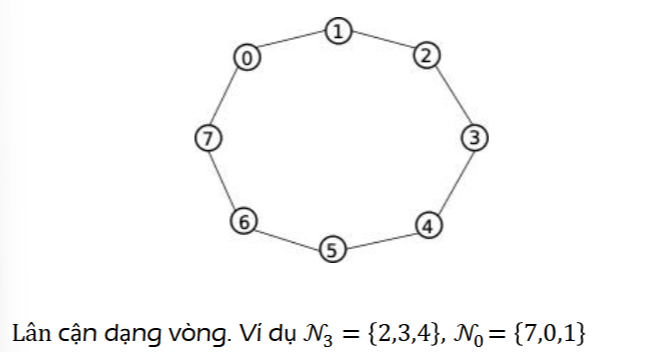
\includegraphics[width=0.75\linewidth]{images/GA-3_21.png}
\end{figure}
$z_{i,g}$ là vị trí tốt nhất từng được tìm ra bởi các phần tử trong lân cận của phần tử đang xét (lân cận bao gồm chính phần tử đó và các phần tử liền kề).

\section{PSO - Lân cận hình sao}

\begin{figure}[H]
    \centering
    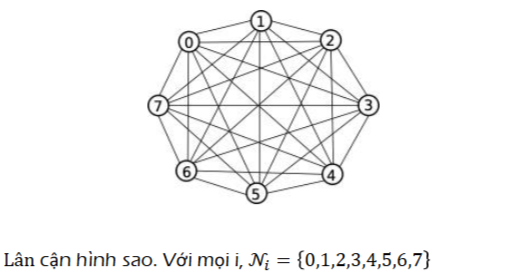
\includegraphics[width=0.75\linewidth]{images/GA-3_22.png}
\end{figure}
$Z_{i,g}$ là vị trí tốt nhất từng được tìm ra tất cả bầy đàn (quần thể).

\section{PSO - Cập nhật vị trí}


\begin{figure}[H]
    \centering
    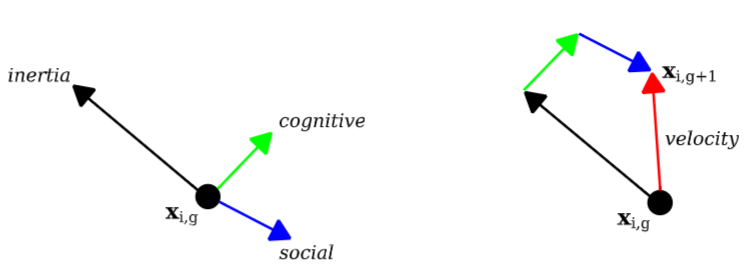
\includegraphics[width=0.75\linewidth]{images/GA-3_23.png}
\end{figure}


\begin{figure}[H]
    \centering
    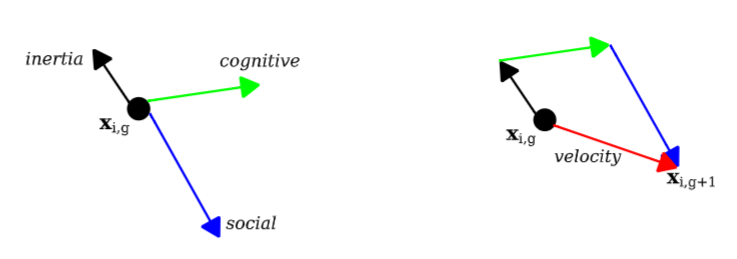
\includegraphics[width=0.75\linewidth]{images/GA-3_24.png}
\end{figure}

\section{PSO - Cập nhật vị trí}

Ở mỗi thế hệ, vector vận tốc của phần tử $i$ được cập nhật:
$$ v_{i,g+1} = wv_{i,g} + c_1r_1\otimes(y_{i,g} - x_{i,g}) + c_2r_2\otimes(z_{i,g} - x_{i,g}) $$
Trong đó:
\begin{itemize}
    \item $w$: Trọng số quán tính.
    \item $c_1, c_2$: Hằng số gia tốc (acceleration constants).
    \item $r_1, r_2$: Vector ngẫu nhiên với các giá trị trong khoảng $(0,1)$.
\end{itemize}

Các thành phần của vector vận tốc (velocity vector):
\begin{itemize}
    \item $wv_{i,g}$: Thành phần \textcolor{red}{quán tính} (inertia)
    \item $c_1r_1\otimes(y_{i,g} - x_{i,g})$: Thành phần \textcolor{red}{nhận thức} (cognitive)
    \item $c_2r_2\otimes(z_{i,g} - x_{i,g})$: Thành phần \textcolor{red}{xã hội} (social)
\end{itemize}

Vị trí kế tiếp của phần tử $i$ được cập nhật bởi:
$$ x_{i,g+1} = x_{i,g} + v_{i,g+1} $$

\section{PSO - Ví dụ - Quan sát 1 phần tử}
\begin{figure}[H]
    \centering
    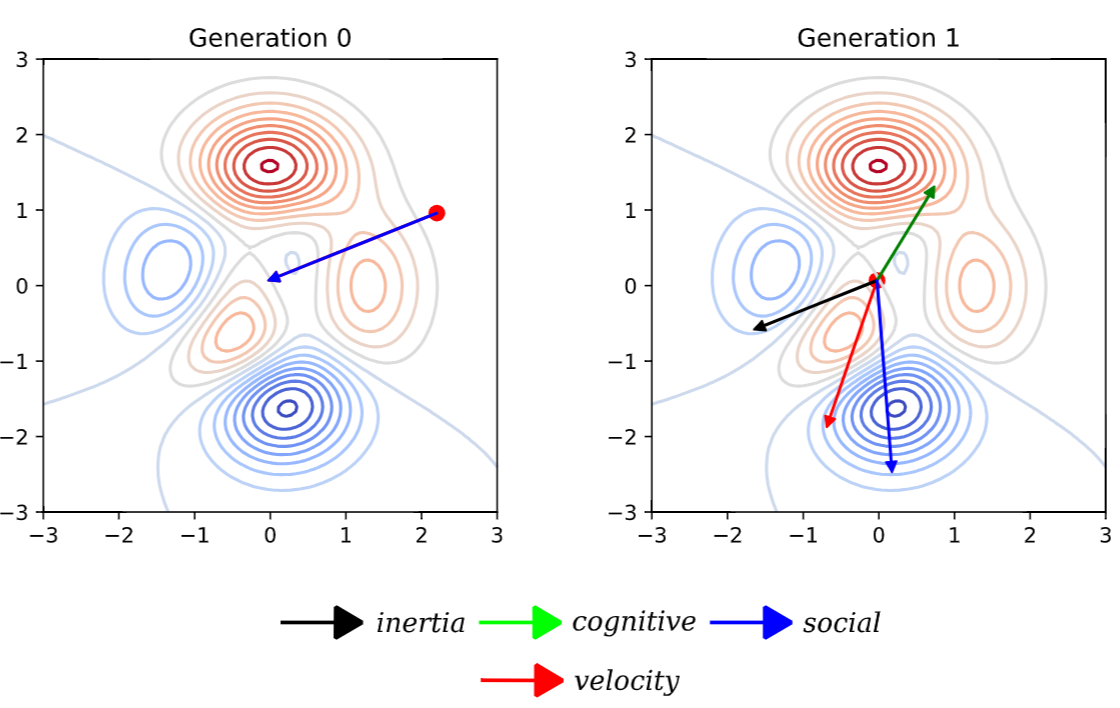
\includegraphics[width=0.75\linewidth]{images/GA-3_45.png}
\end{figure}

\begin{figure}[H]
    \centering
    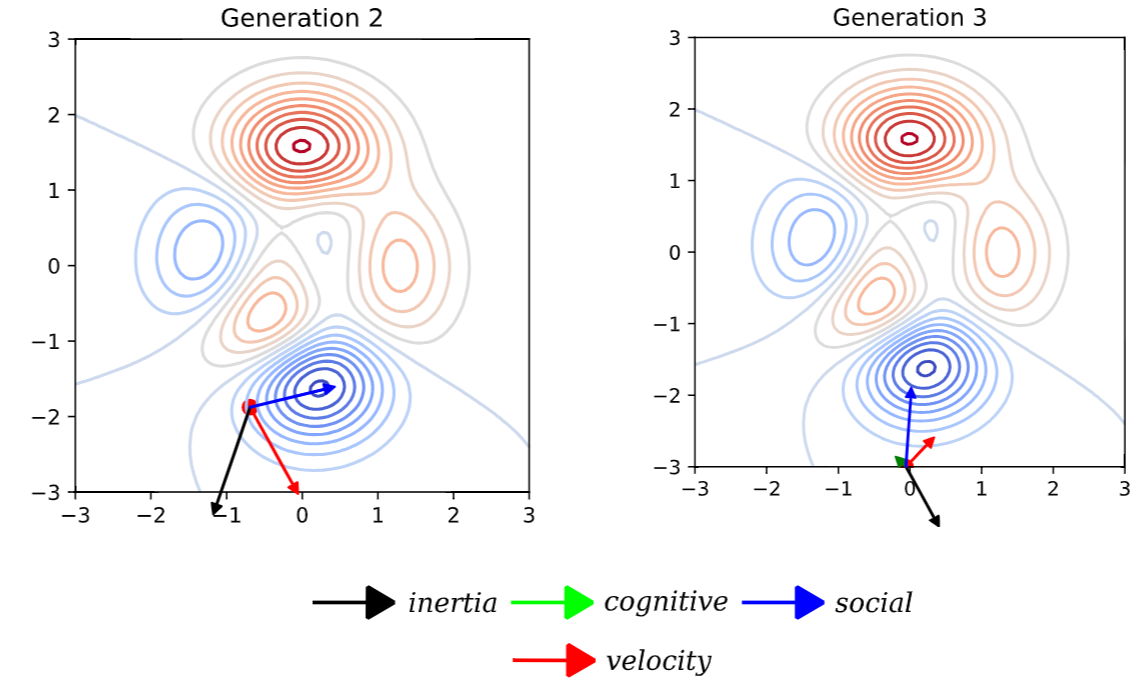
\includegraphics[width=0.75\linewidth]{images/GA-3_46.png}
\end{figure}

\begin{figure}[H]
    \centering
    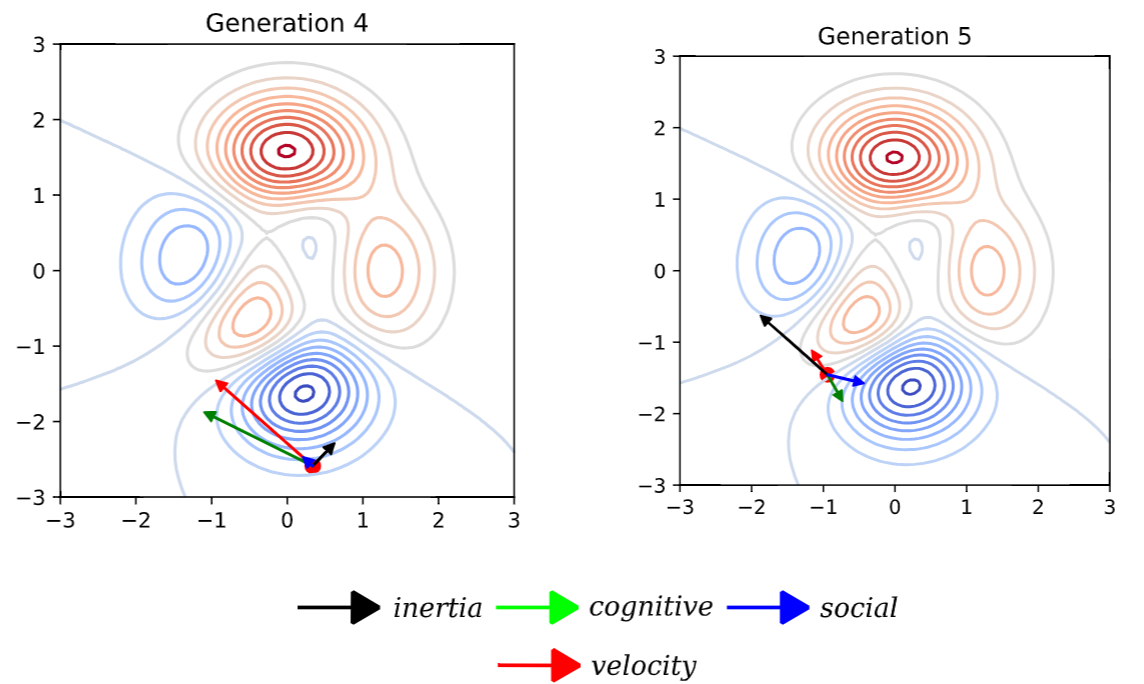
\includegraphics[width=0.75\linewidth]{images/GA-3_57.png}
\end{figure}

\begin{figure}[H]
    \centering
    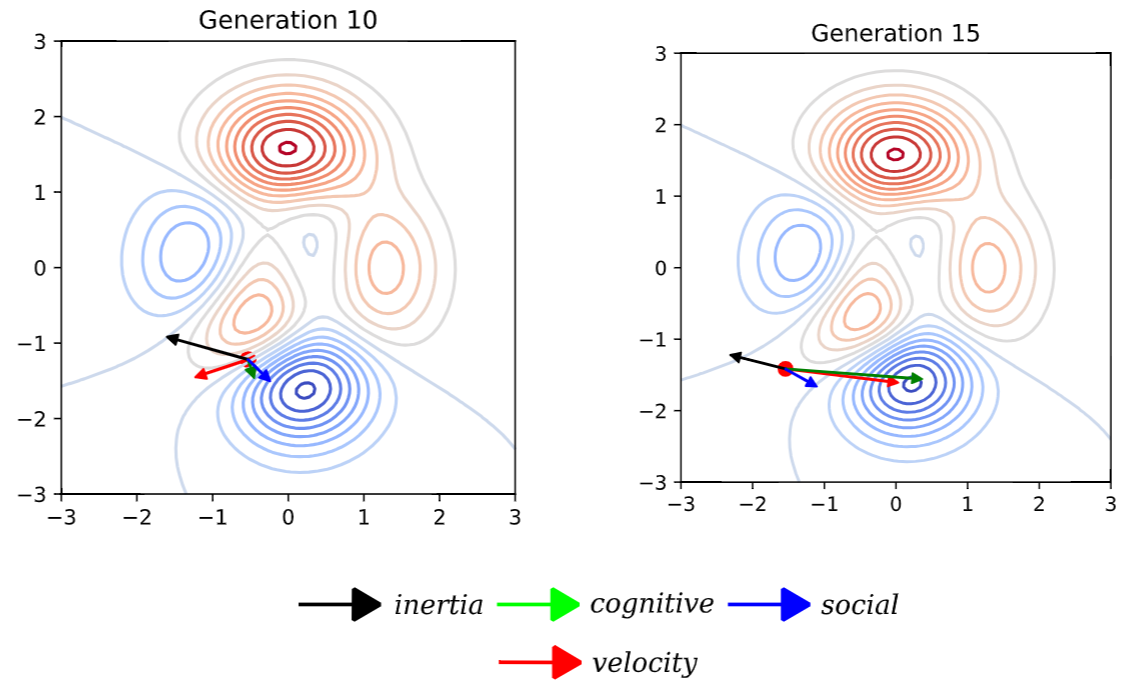
\includegraphics[width=0.75\linewidth]{images/GA-3_48.png}
\end{figure}

\begin{figure}[H]
    \centering
    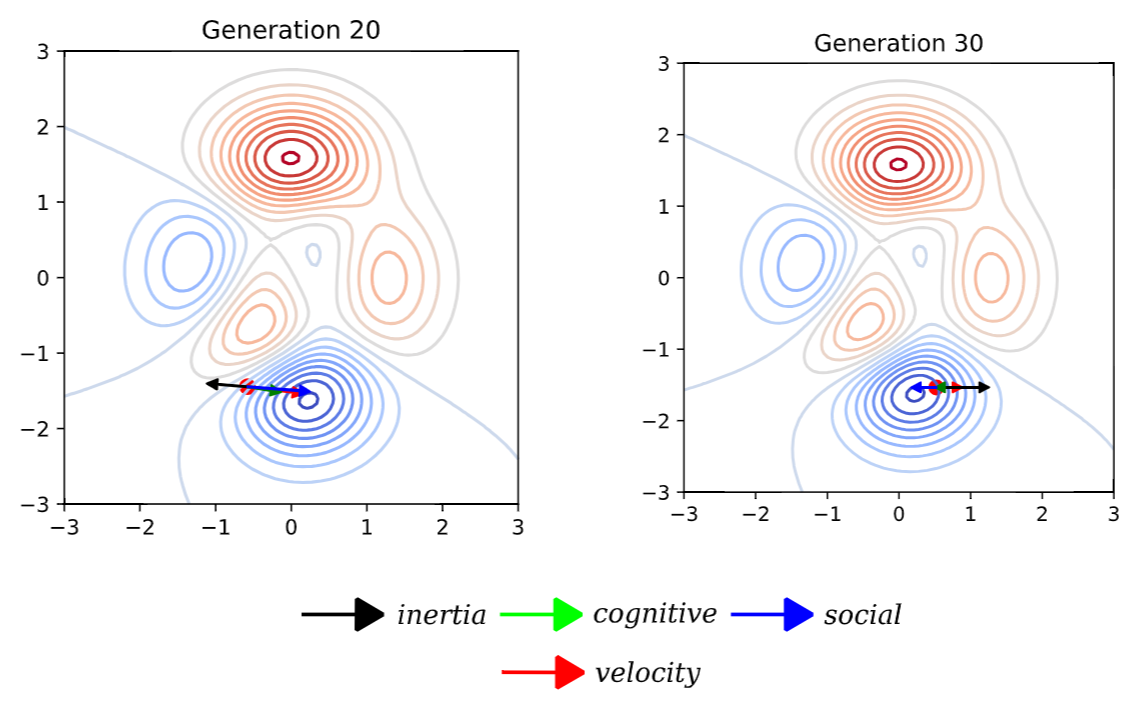
\includegraphics[width=0.75\linewidth]{images/GA-3_49.png}
\end{figure}

\section{PSO - Ví dụ - Quan sát cả bầy đàn}
\begin{figure}[H]
    \centering
    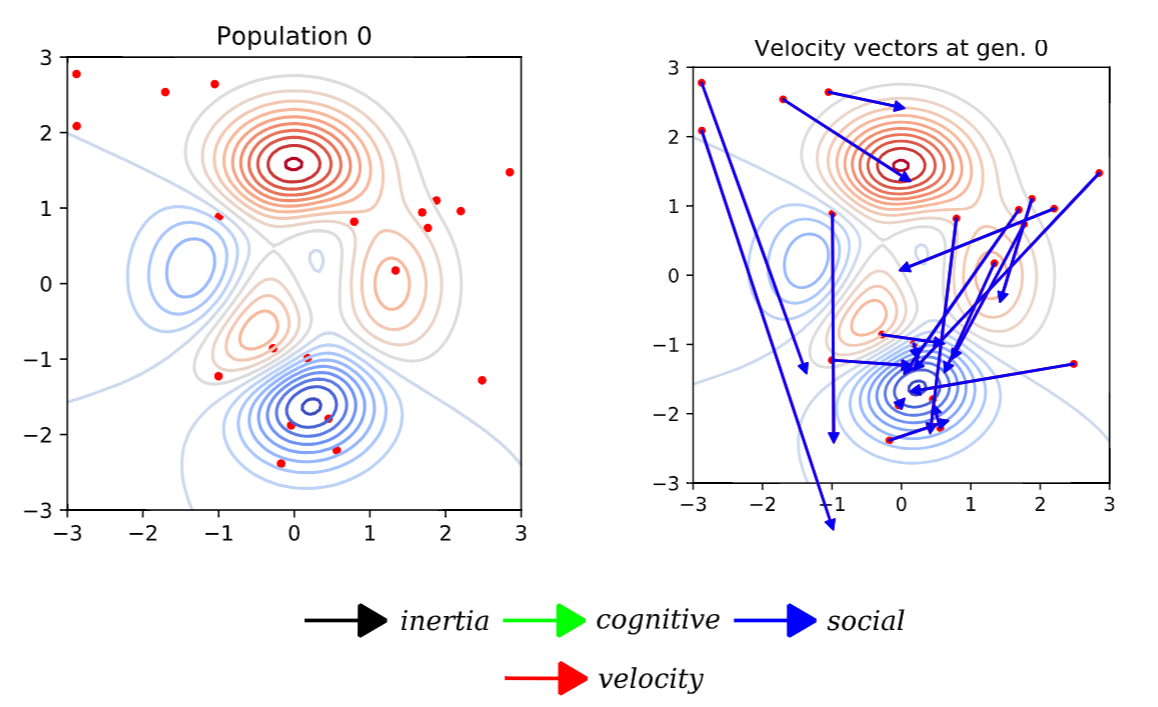
\includegraphics[width=0.75\linewidth]{images/GA-3_50.png}
\end{figure}

\begin{figure}[H]
    \centering
    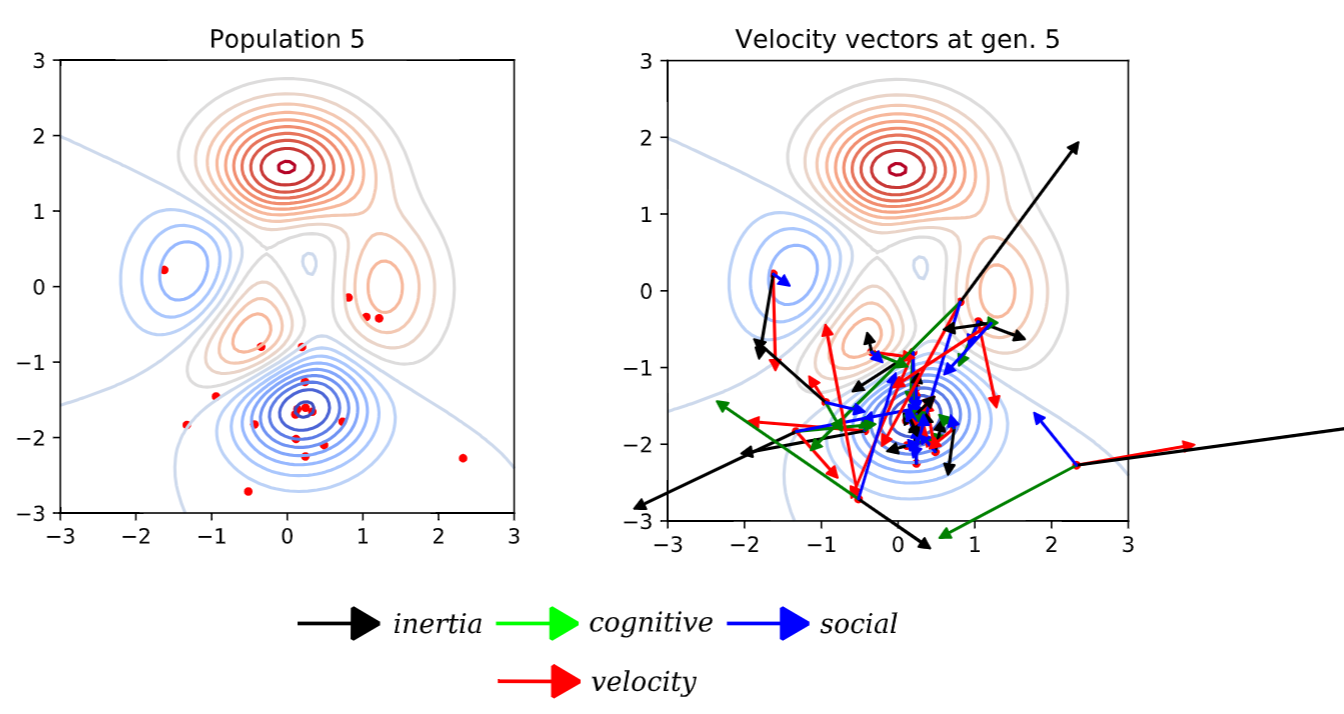
\includegraphics[width=0.75\linewidth]{images/GA-3_51.png}
\end{figure}

\begin{figure}[H]
    \centering
    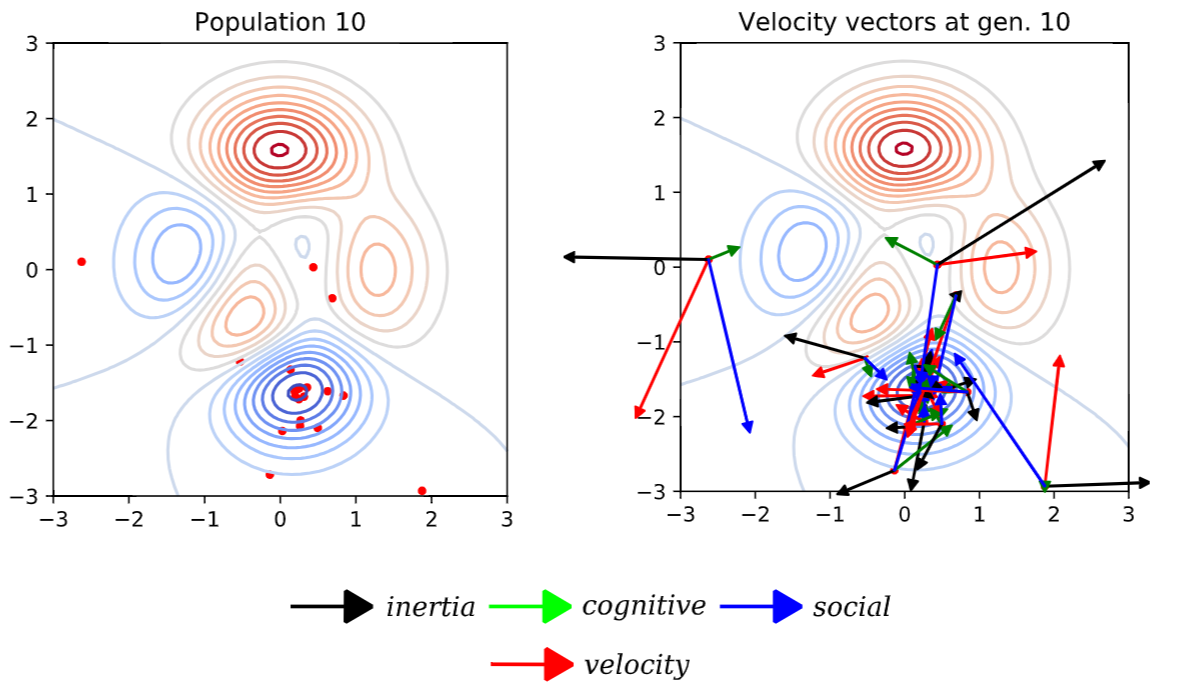
\includegraphics[width=0.75\linewidth]{images/GA-3_52.png}
\end{figure}

\begin{figure}[H]
    \centering
    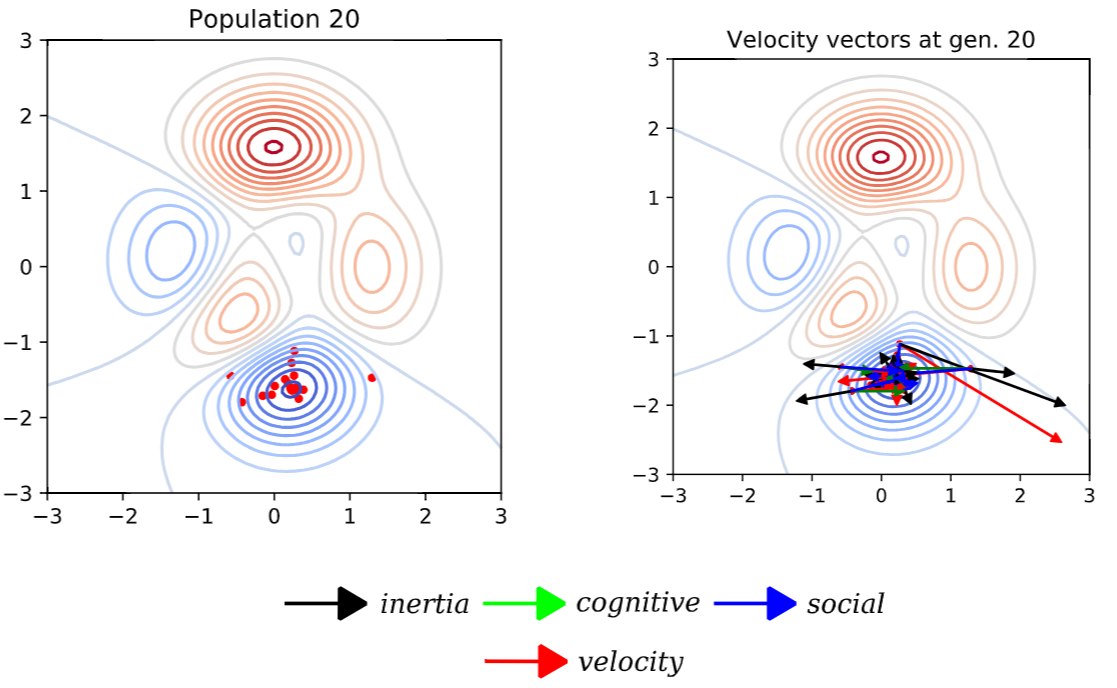
\includegraphics[width=0.75\linewidth]{images/GA-3_53.png}
\end{figure}

\begin{figure}[H]
    \centering
    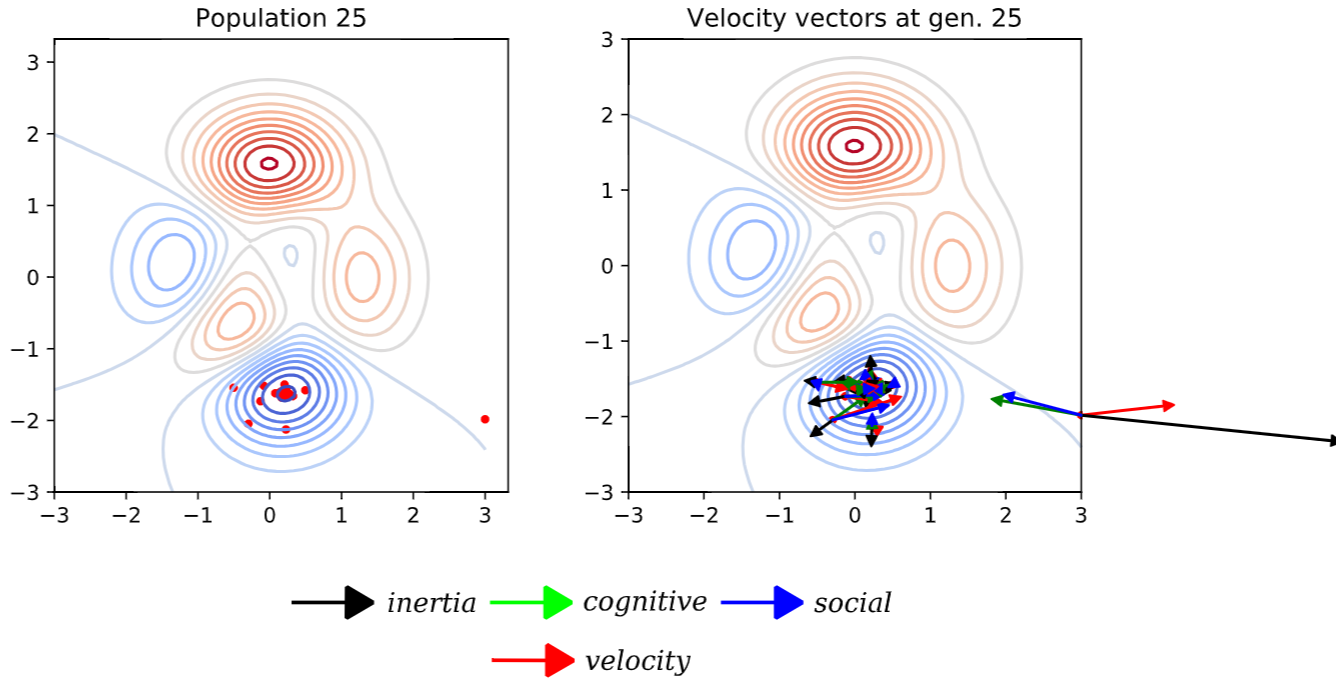
\includegraphics[width=0.75\linewidth]{images/GA-3_54.png}
\end{figure}

\begin{figure}[H]
    \centering
    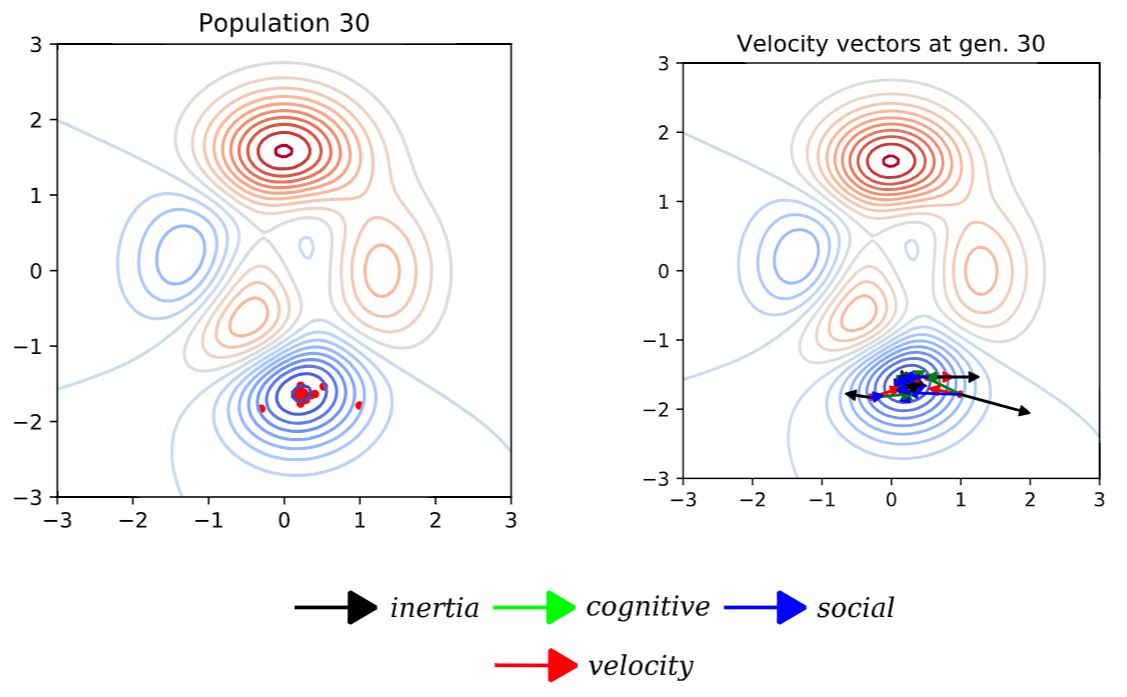
\includegraphics[width=0.75\linewidth]{images/GA-3_55.png}
\end{figure}

\section{PSO - Tham số điều khiển}

\begin{itemize}
    \item Hiệu suất của PSO cũng bị ảnh hưởng lớn bởi các tham số điều khiển:
    \item Kích thước bầy đàn.
    \item Định nghĩa về kiểu lân cận.
    \item Các hệ số: quán tính, gia tốc, ...
\end{itemize}
\chapter{Evolution Strategies (ES) \& Cross-Entropy Methods (CEM)}
\section{Problem Statement}
\begin{itemize}
    \item \textbf{Bài toán}: \textbf{Cực tiểu hóa/Cực đại hóa} một \textbf{hàm mục tiêu} (hàm thích nghi, hàm mất mát) trong miền liên tục.
    \begin{equation*}
        f: X \subseteq \mathbb{R}^n \to \mathbb{R}: x\to f(x)
    \end{equation*}
    \item Kịch bản \textbf{hộp đen} (kịch bản tìm kiếm trực tiếp)
    \begin{itemize}
        \item Gradient không có sẵn hoặc không hữu ích
        \item Kiến thức chuyên biệt về miền vấn đề chỉ được sử dụng bên trong hộp đen
        \begin{figure}[H]
            \centering
            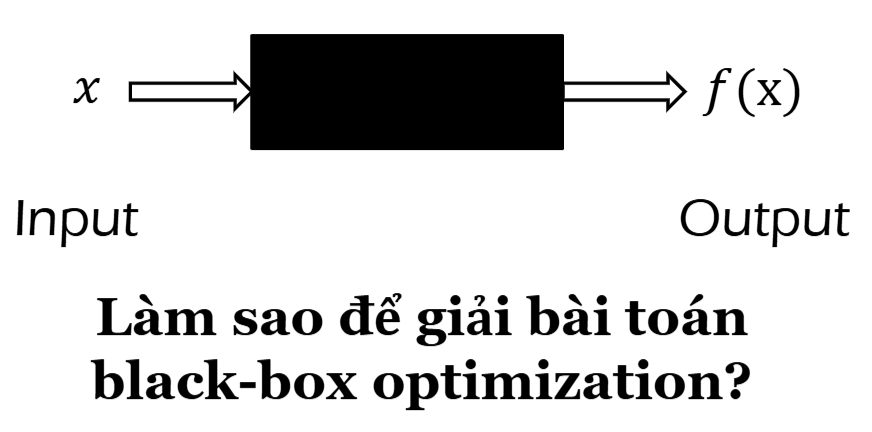
\includegraphics[width=0.5\textwidth]{images/blackbox.png}
            \caption{Minh họa kịch bản tối ưu hóa hộp đen.}
            \label{fig:blackbox-ea}
        \end{figure}
        \item \textbf{Chi phí tìm kiếm}: số lần gọi hàm đánh giá.
        \item \textbf{Mục tiêu}:
        \begin{itemize}
            \item Hội tụ nhanh đến cực tiểu toàn cục hoặc một lời giải $x$ tốt.
            \item Lời giải $x$ tốt với hàm giá trị $f(x)$ nhỏ với chi phí tìm kiếm thấp.
        \end{itemize}
        \item \textbf{Vấn đề}:
        \begin{itemize}
            \item Tìm kiếm vét cạnh (Exhaustive search) gần như không thể.
            \item Tìm kiếm ngẫu nhiên ngây thơ (Naive random search) thì tốn nhiều thời gian.
            \item Tìm kiếm xác định (Deterministic search) thì không thành công/tốn nhiều thời gian.
        \end{itemize}
        \item \textbf{Hướng tiếp cận}: Tìm kiếm xác suất (Stochastic Search), Thuật toán tiến hóa (Evolutionary Algorithms)
        \item Nhưng mọi thứ không dễ ăn như vậy.
        \begin{figure}[H]
            \centering
            \begin{minipage}[c]{0.3\textwidth}
                \centering
                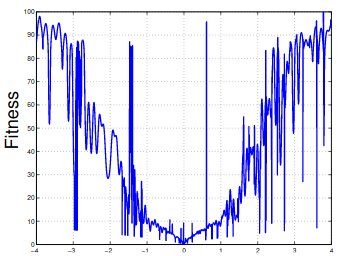
\includegraphics[width=\textwidth]{images/objective_func_1.png}
                \subcaption{Hàm gồ ghề}
            \end{minipage}\hfill
            \begin{minipage}[c]{0.3\textwidth}
                \centering
                \includegraphics[width=\textwidth]{images/objective_func_2.png}
                \subcaption{Hàm có điều kiện xấu}
            \end{minipage}\hfill
            \begin{minipage}[c]{0.3\textwidth}
                \centering
                \includegraphics[width=\textwidth]{images/objective_func_3.png}
                \subcaption{Hàm không phân tách}
            \end{minipage}
            \caption{Một số ví dụ về các hàm mục tiêu phức tạp trong thực tế.}
            \label{fig:objective_func}
        \end{figure}
        \item $f$ trong thực tế có thể:
        \begin{itemize}
            \item Không tuyến tính, phi bậc hai (non-quadratic), không lồi (non-convex)
            \item Tính gồ ghề (Ruggedness)
            \item Tính không phân tách được (Non-separability)
            \item Điều kiện xấu (Ill-conditioning)
            \item Số chiều (kích thước không gian tìm kiếm) lớn hơn ba (Dimensionality larger than three)
        \end{itemize}
    \end{itemize}
\end{itemize}
\section{Tổng quan về ES}
\subsection{Ý tưởng và thuật toán}
\begin{itemize}
    \item Chiến lược tiến hóa (Evolution Strategies - ES): là các kỹ thuật được sử dụng để giải quyết bài toán trong miền liên tục.
    \item Chiến lược tiến hóa: được phát minh (invented) vào đầu những năm 1960 bởi Rechenberg và Schwefel.
    \item Lấy cảm hứng từ chọn lọc tự nhiên.
    \begin{figure}[H]
        \centering
        \includegraphics[width=0.8\textwidth]{images/natural_selection.png}
        \caption{Minh họa chọn lọc tự nhiên.}
    \end{figure}
    \item Chiến lược tiến hóa (Evolution Strategies - ES) thuộc về một họ lớn của các Thuật toán tiến hóa (Evolutionary Algorithms - EA)
    \begin{figure}[H]
        \centering
        \includegraphics[width=0.8\textwidth]{images/family_tree_es.png}
        \caption{Cây phả hệ của các thuật toán tiến hóa, cho thấy vị trí của ES.}
    \end{figure}
    \item Ý tưởng
    \begin{figure}[H]
        \centering
        \includegraphics[width=0.8\textwidth]{images/basic_idea_es.png}
        \caption{Ý tưởng cơ bản của Chiến lược tiến hóa.}
    \end{figure}
\end{itemize}

\subsection{Tái tổ hợp (Recombination)}
\begin{itemize}
    \item \textbf{Tái tổ hợp rời rạc (Discrete Recombination)}
    \begin{itemize}
        \item Tái tổ hợp số học đơn giản (Simple arithmetic Recombination)
        \begin{figure}[H]
            \centering
            \includegraphics[width=0.8\textwidth]{images/simple_arithmetic_recombination.png}
            \caption{Tái tổ hợp số học đơn giản.}
        \end{figure}
        \item Tái tổ hợp số học đơn (Single arithmetic Recombination)
        \begin{figure}[H]
            \centering
            \includegraphics[width=0.8\textwidth]{images/single_arithmetic_recombination.png}
            \caption{Tái tổ hợp số học đơn.}
        \end{figure}
        \item Tái tổ hợp số học toàn phần (Whole arithmetic Recombination)
        \begin{figure}[H]
            \centering
            \includegraphics[width=0.8\textwidth]{images/whole_arithmetic_recombination.png}
            \caption{Tái tổ hợp số học toàn phần.}
        \end{figure}
    \end{itemize}
    \item \textbf{Tái tổ hợp trung gian (Intermediate Recombination)}: Lấy giá trị trung bình của tất cả $\rho$ cha mẹ (tính toán tâm khối, trọng tâm).
    \begin{figure}[H]
        \centering
        \includegraphics[width=0.8\textwidth]{images/intermediate_recombination.png}
        \caption{Tái tổ hợp trung gian.}
    \end{figure}
    \item \textbf{Tái tổ hợp có trọng số (Weighted Recombination)}
    \begin{itemize}
        \item Tái tổ hợp có trọng số là một trường hợp tổng quát của tái tổ hợp trung gian. Nó lấy trung bình có trọng số của $\rho$ cha mẹ.
        \item Các giá trị trọng số phụ thuộc vào thứ hạng độ thích nghi, trong đó các cha mẹ tốt hơn không bao giờ có trọng số nhỏ hơn các cha mẹ kém hơn.
        \begin{figure}[H]
            \centering
            \includegraphics[width=0.8\textwidth]{images/weighted_recombination.png}
            \caption{Tái tổ hợp có trọng số.}
        \end{figure}
    \end{itemize}
\end{itemize}

\subsection{Chọn lọc sống sót (Survivor Selection)}
\begin{itemize}
    \item Được áp dụng để tạo ra $\lambda$ con cái từ $\mu$ cha mẹ thông qua đột biến và tái tổ hợp.
    \item \textbf{Hai cơ chế}: Chọn lọc Plus (ưu tú) và Comma (không ưu tú).
    \begin{itemize}
        \item $(\mu + \lambda)$: chọn $\mu$ cha mẹ mới từ tập hợp gồm cả cha mẹ cũ và con cái.
        \item $(\mu, \lambda)$: chọn $\mu$ cha mẹ mới chỉ từ tập hợp con cái.
        \item $(\mu + \lambda)$ là một chiến lược ưu tú (elitist).
        \item $(\mu, \lambda)$ là một chiến lược chọn lọc cắt cụt (truncation selection).
        \item Chiến lược $(\mu, \lambda)$ thường được ưa chuộng hơn vì:
        \begin{itemize}
            \item Tốt hơn trong việc thoát khỏi điểm tối ưu cục bộ.
            \item Tốt hơn trong việc theo dõi điểm tối ưu di động.
            \item Với chọn lọc "plus", các tham số chiến lược tồi có thể tồn tại trong quần thể quá lâu nếu một cá thể có các biến mục tiêu tương đối tốt.
        \end{itemize}
    \end{itemize}
\end{itemize}

\subsection{Đột biến (Mutation)}
\begin{itemize}
    \item Toán tử đột biến tạo ra các biến thể ("nhỏ") bằng cách thêm một nhiễu loạn đối xứng điểm vào kết quả của tái tổ hợp. 
    \begin{equation*}
        m'=m+\sigma\mathcal{N}(0,\mathbf{C})
    \end{equation*}
    \begin{figure}[H]
        \centering
        \begin{minipage}[c]{0.3\textwidth}
            \centering
            \includegraphics[width=\textwidth]{images/spherical_mutation.png}
            \subcaption{Dạng cầu (Spherical)}
        \end{minipage}\hfill
        \begin{minipage}[c]{0.3\textwidth}
            \centering
            \includegraphics[width=\textwidth]{images/axis_parallel_mutation.png}
            \subcaption{Song song với trục (Axis-parallel)}
        \end{minipage}\hfill
        \begin{minipage}[c]{0.3\textwidth}
            \centering
            \includegraphics[width=\textwidth]{images/general_mutation.png}
            \subcaption{Dạng tổng quát (General)}
        \end{minipage}
        \caption{Minh họa các dạng đột biến trong ES.}
        \label{fig:mutation_types}
    \end{figure}
\end{itemize}
\subsection{Kiểm soát tham số (Parameters Control)}
\begin{itemize}
    \item Kiểm soát các tham số của toán tử đột biến là chìa khóa trong thiết kế chiến lược tiến hóa và ảnh hưởng đến tốc độ hội tụ.
    \begin{figure}[H]
        \centering
        \includegraphics[width=0.8\textwidth]{images/step_size_effect_convergence.png}
        \caption{Kích thước bước ảnh hưởng đến sự hội tụ (Step-size affects convergence)}
        \label{fig:step_size_effect_convergence}
    \end{figure}
    \item Quy tắc thành công 1/5 (1/5-th success rule), thường được áp dụng với chọn lọc Plus (Plus-selection)
    \begin{itemize}[nosep]
        \item tăng kích thước bước nếu hơn 20\% giải pháp mới thành công, ngược lại thì giảm
    \end{itemize}
    \vspace{-0.1cm}
    \item Tự thích nghi $\sigma$ ($\sigma$-self-adaptation), được áp dụng với chọn lọc Comma (Comma-selection)
    \begin{itemize}[nosep]
        \item đột biến được áp dụng cho kích thước bước và giải pháp tốt hơn, dựa trên giá trị hàm mục tiêu, sẽ được chọn
    \end{itemize}
    \item Kiểm soát độ dài đường đi (Thích ứng kích thước bước tích lũy - Cummulative Step-size Adaptation, CSA)
    \begin{itemize}[nosep]
        \item tự thích nghi được khử ngẫu nhiên và không cục bộ hóa
    \end{itemize}
    \item Thuật toán (1 + 1)ES
    \begin{algorithm}[]
        \caption{(1 + 1)ES}
        \label{alg:oneplusone_es}
        \begin{algorithmic}[1]
        \STATE \textbf{Hyperparameters:} $c_{inc} > 0, c_{dec} > 0$
        \STATE \textbf{Input:} vector $m^{(0)} \in \mathbb{R}^d$, step-size $\sigma^{(0)} \in \mathbb{R}_{>0}$
        \STATE 
        \vspace{1mm}
        \FOR{$t = 0, \dots, T - 1$}
            \STATE \parbox[c]{\dimexpr\linewidth-2.5em}{% Using a parbox to group the description and equations under one line number
            Create 1 offspring by adding a point symmetric perturbation to $m^{(t)}$
            \vspace{0.2em}
            \begin{center}
            $(\epsilon^{(t)}) \sim \mathcal{N}(0, \mathbf{I}_d)$ \\
            $x^{(t)} \leftarrow m^{(t)} + \sigma^{(t)}\epsilon^{(t)}$
            \end{center}
            }
            \STATE Survival selection (1 + 1) and update step-size
            \IF{$F(x^{(t)}) \le F(m^{(t)})$}
                \STATE $m^{(t+1)} \leftarrow x^{(t)}$
                \STATE $\sigma^{(t+1)} \leftarrow \sigma^{(t)}c_{inc}$
            \ELSE
                \STATE $m^{(t+1)} \leftarrow m^{(t)}$
                \STATE $\sigma^{(t+1)} \leftarrow \sigma^{(t)}c_{dec}$
            \ENDIF
        \ENDFOR
        \end{algorithmic}
    \end{algorithm}
    \item \textbf{Hàm kiểm thử (Test Function)}
    \begin{figure}[H]
        \centering
        \begin{minipage}[c]{0.45\textwidth}
            \centering
            \includegraphics[width=\textwidth]{images/sphere_function_3D.png}
            \caption{Hàm Sphere trong không gian 3 chiều (Sphere Function in 3D)}
            \label{fig:sphere_function}
        \end{minipage}
        \begin{minipage}[c]{0.45\textwidth}
            \begin{itemize}
                \item[] \textbf{Công thức (Formula)}: $f(x)=x_1^2+x_2^2$
                \item[] \textbf{Miền tìm kiếm (Search domain)}: $\infty\leq x_i\leq \infty, \ 1\leq i\leq2$
                \item[] \textbf{Cực tiểu toàn cục (Global Minimum)}: $f(x)=f(0)=0$
            \end{itemize}
        \end{minipage}
    \end{figure}
    \begin{figure}[H]
        \begin{figure}[H]
            \begin{minipage}[c]{0.3\textwidth}
                \centering
                \includegraphics[width=\textwidth]{images/one_plus_one_ex_step_0.png}
            \end{minipage}
            \begin{minipage}[c]{0.3\textwidth}
                \centering
                \includegraphics[width=\textwidth]{images/one_plus_one_ex_step_1.png}
            \end{minipage}
            \begin{minipage}[c]{0.3\textwidth}
                \centering
                \includegraphics[width=\textwidth]{images/one_plus_one_ex_step_2.png}
            \end{minipage}
        \end{figure}
        \begin{figure}[H]
            \begin{minipage}[c]{0.3\textwidth}
                \centering
                \includegraphics[width=\textwidth]{images/one_plus_one_ex_step_3.png}
            \end{minipage}
            \begin{minipage}[c]{0.3\textwidth}
                \centering
                \includegraphics[width=\textwidth]{images/one_plus_one_ex_step_4.png}
            \end{minipage}
            \begin{minipage}[c]{0.3\textwidth}
                \centering
                \includegraphics[width=\textwidth]{images/one_plus_one_ex_step_5.png}
            \end{minipage}
        \end{figure}
            \begin{figure}[H]
            \begin{minipage}[c]{0.45\textwidth}
                \centering
                \includegraphics[width=\textwidth]{images/one_plus_one_ex_step_6.png}
            \end{minipage}
            \begin{minipage}[c]{0.45\textwidth}
                \centering
                \includegraphics[width=\textwidth]{images/one_plus_one_ex_step_7.png}
            \end{minipage}
        \end{figure}
        \caption{Ví dụ thuật toán (1 + 1)ES trên hàm Sphere (thể hiện ở hình~\ref{fig:sphere_function}).}
        \label{fig:one_plus_one_ex}
    \end{figure}
    \item Thuật toán (1 + 1)ES
    \begin{algorithm}[]
        \caption{(1 + $\lambda$)ES}
        \label{alg:onepluslambda_es}
        \begin{algorithmic}[1]
        \STATE \textbf{Hyperparameters:} $c_{inc} > 0, c_{dec} > 0$
        \STATE \textbf{Input:} vector $m^{(0)} \in \mathbb{R}^d$, step-size $\sigma^{(0)} \in \mathbb{R}_{>0}$, number of offspring $\lambda>0$
        \STATE 
        \vspace{1mm}
        \FOR{$t = 0, \dots, T - 1$}
            \STATE \parbox[c]{\dimexpr\linewidth-2.5em}{% Using a parbox to group the description and equations under one line number
            Create $\lambda$ offspring by adding a point symmetric perturbation to $m^{(t)}$
            \vspace{0.2em}
            \begin{center}
                $(\epsilon^{(t)_i})_{i=1,\dots,\lambda} \sim \mathcal{N}(0, \mathbf{I}_d)$ \\
                $x^{(t)}_i \gets m^{(t)} + \sigma^{(t)}\epsilon^{(t)}_i, \ i=1,\dots,\lambda$
            \end{center}
            }
            \STATE Find the best solution in the offspring
            \begin{center}
                $x_{best}^{(t)}=\underset{x_{i}^{(t)}\in \operatorname{offspring}}{\arg\min}F(x_i^{(t)})$
            \end{center}
            \IF{$F(x_{best}^{(t)}) \leq F(m^{(t)})$}
                \STATE $m^{(t+1)}\gets x_{best}^{(t)}$
                \STATE $m^{(t+1)}\gets x_{best}^{(t)}$
                \STATE $\sigma^{(t+1)}\gets \sigma^{(t)}c_{inc}$

            \ELSE
                \STATE $m^{(t+1)}\gets m^{(t)}$
                \STATE $\sigma^{(t+1)}\gets \sigma^{(t)}c_{dec}$
                \ENDIF
        \ENDFOR
        \end{algorithmic}
    \end{algorithm}
    \begin{figure}[H]
        \begin{figure}[H]
            \begin{minipage}[c]{0.3\textwidth}
                \centering
                \includegraphics[width=\textwidth]{images/one_plus_lambda_ex_step_0.png}
            \end{minipage}
            \begin{minipage}[c]{0.3\textwidth}
                \centering
                \includegraphics[width=\textwidth]{images/one_plus_lambda_ex_step_1.png}
            \end{minipage}
            \begin{minipage}[c]{0.3\textwidth}
                \centering
                \includegraphics[width=\textwidth]{images/one_plus_lambda_ex_step_2.png}
            \end{minipage}
        \end{figure}
        \begin{figure}[H]
            \begin{minipage}[c]{0.3\textwidth}
                \centering
                \includegraphics[width=\textwidth]{images/one_plus_lambda_ex_step_3.png}
            \end{minipage}
            \begin{minipage}[c]{0.3\textwidth}
                \centering
                \includegraphics[width=\textwidth]{images/one_plus_lambda_ex_step_4.png}
            \end{minipage}
            \begin{minipage}[c]{0.3\textwidth}
                \centering
                \includegraphics[width=\textwidth]{images/one_plus_lambda_ex_step_5.png}
            \end{minipage}
        \end{figure}
            \begin{figure}[H]
            \begin{minipage}[c]{0.45\textwidth}
                \centering
                \includegraphics[width=\textwidth]{images/one_plus_lambda_ex_step_6.png}
            \end{minipage}
            \begin{minipage}[c]{0.45\textwidth}
                \centering
                \includegraphics[width=\textwidth]{images/one_plus_lambda_ex_step_7.png}
            \end{minipage}
        \end{figure}
        \caption{Ví dụ thuật toán (1 + $\lambda$)ES trên hàm Sphere (thể hiện ở hình~\ref{fig:sphere_function}).}
        \label{fig:one_plus_lambda_ex}
    \end{figure}
    \begin{algorithm}[]
        \caption{($\mu/\rho,^{+},\lambda$)-Self-Adapation ES}
        \label{alg:mu_rho_lambda_es}
        \begin{algorithmic}[1]
            \STATE \textbf{Input:} $\rho, \lambda, \mu \in \mathbb{N}_{+}$
            \STATE \textit{Initialize} ($\mathcal{P}_{\mu}^{0}\gets \{(x_i^0,\text{s}_i^{0}, F(x_i^0)), \ i=1,2,\dots,\mu\}$)
            \STATE $g \gets 0$
            \WHILE {$Termination\_Condition is not statisfied$}
                \STATE $\tilde{\mathcal{P}}_{\lambda}^{g}\gets 0$
                \FOR{$i\gets 1$;$\mu$}
                    \STATE $(x_i,\text{s}_i)\gets \textbf{recombine(select\_mates)}(\mathcal{P}_{\mu}^{g},\rho)$
                    \STATE $\tilde{\text{s}}_i\gets \textbf{s\_mutation}(\text{s}_i)$
                    \STATE $\tilde{\text{x}}_i\gets \textbf{x\_mutation}(\text{x}_i)$
                    \STATE $\tilde{F}_i\gets F(\tilde{x}_i)$
                \ENDFOR
                \STATE $\tilde{\mathcal{P}}_{\lambda}^g\gets \{(\tilde{x}_i, \tilde{\text{s}}_i, \tilde{F}_i), \ i=1,\dots,\lambda\}$
                \STATE $\mathcal{P}_{\mu}^{g+1}\gets)\}$
                \SWITCH {$selection\_type$}
                    \CASE{($\mu, \lambda$)}
                        \STATE $\mathcal{P}_{\mu}^{g+1}\gets \textbf{selection}(\tilde{\mathcal{P}}_{\lambda}^g, \mu)$
                    \ENDCASE
                    \CASE{($\mu, \rho$)}
                        \STATE $\mathcal{P}_{\mu}^{g+1}\gets \textbf{selection}(\tilde{\mathcal{P}}_{\lambda}^g, \mathcal{P}_{\mu}^g, \mu)$
                    \ENDCASE
                \ENDSWITCH
                \STATE $g\gets g+1$
            \ENDWHILE
        \end{algorithmic}
    \end{algorithm}
\end{itemize}
\vspace{-0.79cm}
\begin{table}[]
    \centering
    \begin{tabular}{|c|c|}
        \toprule
        \multicolumn{2}{|c|}{\textbf{Summary}} \\
        \midrule
        \textbf{Encoding} & \textbf{Real vectors} \\
        \midrule
        Recombination & Discrete or intermediate \\
        Mutation & Random additive perturbation (uniform, Gaussian, Cauchy) \\
        Parents selection & Uniformly random \\
        Survivors selection & ($\mu, \lambda$) or ($\mu + \lambda$) \\
        Particularity & Self-adaptive mutation parameters \\
        \bottomrule
    \end{tabular}
\end{table}
\section{CEM}
\begin{algorithm}[]
\caption{CEM}
\label{alg:cem}
\begin{algorithmic}[1]
    \STATE \textbf{Hyperparameters:} $\sigma_{init} \in \mathbb{R}_{>0}$
    \STATE \textbf{Input:} function $F$, vector $\mu_0 \in \mathbb{R}^d$,
    \STATE number of sample $N$, number of elite set $N_e$
    \STATE \textbf{Initialize:} $\Sigma_0 = \sigma_{init}\mathbf{I}_d$
    \STATE
    \FOR{$t = 0, \dots, T-1$}
        \STATE Sample $N$ search points $x_1, \dots, x_N$ from $\mathcal{N}(\mu_t, \Sigma_t)$
        \STATE Evaluate the samples $x_1, \dots, x_N$ on $F$
        \STATE Select top $N_e$ search points $(z_i)_{i=1, \dots, N_e}$
        \STATE Update the parameters of the distribution 
        \begin{center}
            $\displaystyle \mu_{t+1} = \frac{1}{N_{\epsilon}} \sum_{i=1}^{N_{\epsilon}} z_i$ \\
            $\displaystyle \Sigma_{t+1} = \frac{1}{N_{\epsilon}} \sum_{i=1}^{N_{\epsilon}} (z_i - \mu_{t+1})(z_i - \mu_{t+1})^T$
        \end{center}
    \ENDFOR
\end{algorithmic}
\end{algorithm}
\begin{itemize}
    \item \textbf{Some modify to prevent premature convergence}
\end{itemize}
\begin{algorithm}
\caption{CEM (Modified)}
\label{alg:cem_modified}
    \begin{algorithmic}[1]
        \STATE \textbf{Hyperparameters:} extra variance $\epsilon$; $\sigma_{init} \in \mathbb{R}_{>0}$
        \STATE \textbf{Input:} function $F$, vector $\mu_0 \in \mathbb{R}^d$,
        \STATE number of sample $N$, number of elite set $N_e$,
        \STATE \textbf{Initialize:} $\Sigma_0 = \sigma_{init} \mathbf{I}_d$
        \begin{center}
        $(w_i)_{i=1,...,N_e}$, where $w_i = \frac{1}{N_e}$ \\
         or $w_i = \frac{\log(N_e+1) - \log(i)}{\sum_{i=1}^{N_e} \log(N_e+1) - \log(i)}$
        \end{center}
        \FOR{$t = 0, \dots, T-1$}
            \STATE Sample $N$ search points $x_1, \dots, x_N$ from $\mathcal{N}(\mu_t, \Sigma_t)$
            \STATE Evaluate the samples $x_1, \dots, x_N$ on $F$
            \STATE Select top $N_e$ search points $(z_i)_{i=1,...,N_e}$
            \STATE Update the parameters of the distribution
            \begin{align*}
                \mu_{t+1} &= \sum_{i=1}^{N_e} w_i z_i \\
                \Sigma_{t+1} &= \sum_{i=1}^{N_e} w_i (z_i - \mu_t)(z_i - \mu_t)^T + \epsilon \mathbf{I}_d
            \end{align*}
        \ENDFOR
    \end{algorithmic}
\end{algorithm}
\section{CMA-ES}
\subsection{Sampling}
\begin{figure}[H]
    \centering
    \includegraphics[width=0.45\textwidth]{images/sampling.png}
\end{figure}
\begin{figure}[H]
    \centering
    \begin{minipage}[t]{0.45\textwidth} 
        \vspace{0pt} 
        \begin{itemize}
            \item Các điểm tìm kiếm mới được tạo ra bằng cách lấy mẫu từ một phân phối chuẩn đa biến:
            \begin{equation*}
                \begin{aligned}
                \mathbf{x}_k^{(g+1)}\sim \mathbf{m}^{(g)}+\sigma^{(g)}\mathcal{N}(0, \mathbf{C}^{(g)}), \\ \forall k=1,\dots,\lambda 
                \end{aligned}
            \end{equation*}
            \item Trong đó:
            \begin{itemize}
                \item Kích thước bước (z) $\sigma \in \mathbb{R}_{+}$ kiểm soát độ dài bước.
                \item Ma trận hiệp phương sai $\mathbf{C}\in \mathbb{R}^{n\times n}$ xác định hình dạng của ellipsoid phân phối.
            \end{itemize}
        \end{itemize}
    \end{minipage}\hfill 
    \begin{minipage}[t]{0.45\textwidth} 
        \vspace{0pt} 
        \centering
        \includegraphics[width=\textwidth]{images/sampling_2.png}
    \end{minipage}
    \caption{Quá trình lấy mẫu trong CMA-ES: các điểm mới được tạo từ phân phối chuẩn đa biến được xác định bởi trung bình $m^{(g)}$, kích thước bước $\sigma^{(g)}$, và ma trận hiệp phương sai $C^{(g)}$.}
    \label{fig:cmaes_sampling_process} 
\end{figure}
\begin{itemize}
    \item Why Normal Distribution ?
    \begin{itemize}
        \item Approximates many natural phenomena so well
        \item Only stable distribution with finite variance
        \item Most convenient way to generate isotropic search points
        \item Maximum entropy distribution with finite variance
    \end{itemize}
\end{itemize}
\subsection{Selection and Recombination}
\begin{itemize}
    \item Giá trị mean mới được tính bằng
    \begin{equation*}
        \begin{aligned} 
            \mathbf{m}^{(g+1)} &= \mathbf{m}^{(g)} + c_m \sum_{i=1}^{\lambda} w_i (\mathbf{x}^{(g+1)}_{i:\lambda} - \mathbf{m}^{(g)}) \\
            \sum_{i=1}^{\mu} w_i &= 1, \quad w_1 \geq w_2 \geq \dots \geq w_\mu > 0
        \end{aligned}
    \end{equation*}
    \item[] Trong đó:
    \begin{itemize}
        \item $c_m\leq 1$ là một tốc độ học (learning rate), thường được đặt bằng 1.
        \item $w_{i=1,\dots,\mu}\in\mathbb{R}_{>0}$ là các hệ số trọng số dương cho tái tổ hợp.
        \item $\{x_{i:\lambda} \mid i=1,\ldots,\lambda\}$ là tập hợp các cá thể $\{x_i \mid i=1,\dots,\lambda\}$ đã được sắp xếp sao cho $f(x_{1:\lambda})\leq\dots\leq f(x_{\mu:\lambda})\leq f(x_{\mu+1:\lambda})\leq \dots,$
    \end{itemize}
    \item Tái tổ hợp trung gian (Intermediate recombination):
    \begin{equation*}
        w_{m}:= \begin{cases}
            \frac{1}{\mu}, & \text{cho } 1 \leq m \leq \mu, \\
            0, & \text{ngược lại}.
        \end{cases}
    \end{equation*}
    \item Tái tổ hợp có trọng số (Weighted recombination):
    \begin{equation*}
        \begin{aligned}
            w_m &:= \begin{cases}
                \frac{\ln{\frac{\lambda+1}{2}}-\ln{m}}{\sum_{k=1}^{\mu}(\ln(\frac{\lambda+1}{2})-\ln{k})}, & \text{for } 1\leq m\leq \mu \\
                0, & \text{ngược lại}
            \end{cases} \\
            \mu_{\operatorname{eff}} &= \left(\frac{\|w\|_1}{\|w\|_2}\right)^2 = \frac{\|w\|_1^2}{\|w\|_2^2} = \frac{(\sum_{i=1}^\mu{|w_i|})^2}{\sum_{i=1}^{\mu}{w_i^2}} = \frac{1}{\sum_{i=1}^{\mu}w_i^2}
        \end{aligned}
    \end{equation*}
    \begin{figure}[H]
        \centering
        \includegraphics[width=\textwidth]{images/selection_and_recombination.png}
        \caption{Ví dụ về chọn lọc và tái tổ hợp (Selection and Recombination example)}
        \label{fig:selection_and_recombination}
    \end{figure}
\end{itemize}
\subsection{Thích ứng Ma trận Hiệp phương sai (Adapting the Covariance Matrix)}
    \begin{itemize}
        \item Việc thích ứng ma trận hiệp phương sai tương đương với việc học một mô hình bậc hai của hàm mục tiêu cơ sở, tương tự như việc xấp xỉ ma trận Hessian nghịch đảo trong phương pháp quasi-Newton của tối ưu hóa cổ điển.
        \begin{figure}[H]
            \centering % Thêm centering cho cả cụm minipage
            \begin{minipage}[c]{0.45\textwidth}
                \centering
                \includegraphics[width=0.75\textwidth]{images/adapting_the_covariance_matrix_1.png}
            \end{minipage}\hfill % Thêm hfill để đẩy các minipage ra xa nhau
            \begin{minipage}[c]{0.45\textwidth}
                \centering
                \includegraphics[width=0.75\textwidth]{images/adapting_the_covariance_matrix_2.png}
            \end{minipage}
            % Có thể thêm caption cho figure này nếu cần
        \end{figure}
        \begin{equation*}
            \begin{aligned}
                &\frac{\partial}{\partial \mathbf{x}}f(\mathbf{x}_i+\Delta\mathbf{x}) = 0 \\
                &\Leftrightarrow\underbrace{\frac{\partial}{\partial \mathbf{x}}f(\mathbf{x}_i)}_{\operatorname{Gradient}}+\underbrace{\frac{\partial^2}{\partial \mathbf{x}^2}f(\mathbf{x}_i)\Delta\mathbf{x}}_{\operatorname{Hessian}}=0 \\ % Sửa ký hiệu đạo hàm bậc hai
                % Dòng dưới có vẻ lặp lại, có thể bỏ nếu không cần thiết
                % &\Leftrightarrow\frac{\partial}{\partial \mathbf{x}}f(\mathbf{x}_i+\Delta \mathbf{x}) = 0 \\ 
                &\Leftrightarrow \mathbf{g}+\mathbf{H}\Delta\mathbf{x}=0 \\
                &\Leftrightarrow\Delta\mathbf{x}=-\mathbf{H}^{-1}\mathbf{g}
            \end{aligned}
        \end{equation*}
        \item Ước lượng phương sai của phân phối trong các điểm đã lấy mẫu:
        \begin{equation*}
            \mathbf{C}^{(g+1)}_{\text{EMNA}_{\text{global}}}=\frac{1}{(\sigma^{(g)})^2}\sum_{i=1}^{\mu}w_i(\mathbf{x}_{i:\lambda}^{(g+1)}-\mathbf{m}^{(g+1)})(\mathbf{x}_{i:\lambda}^{(g+1)}-\mathbf{m}^{(g+1)})^T
        \end{equation*}
        \item Ước lượng phương sai của các bước đã lấy mẫu:
        \begin{equation*}
            \mathbf{C}^{(g+1)}_{\mu}=\frac{1}{(\sigma^{(g)})^2}\sum_{i=1}^{\mu}w_i(\mathbf{x}_{i:\lambda}^{(g+1)}-\mathbf{m}^{(g)})(\mathbf{x}_{i:\lambda}^{(g+1)}-\mathbf{m}^{(g)})^T
        \end{equation*}
        \begin{figure}[H] % Đã có H]
            \centering
            \includegraphics[width=\textwidth]{images/estimating_the_covariance_matrix.png}
            \caption{Ước lượng Ma trận Hiệp phương sai (Estimating the Covariance Matrix)}
            \label{fig:estimating_the_covariance_matrix} % Sửa lỗi chính tả "estiamting" -> "estimating"
        \end{figure}
        \item Cập nhật Rank-$\mu$ (Rank-$\mu$-Update): Để đạt được tìm kiếm nhanh, kích thước quần thể phải nhỏ:
        \begin{itemize}
            \item[] $\Rightarrow$ Do đó, việc có được một bộ ước lượng đáng tin cậy cho ma trận hiệp phương sai tốt (chỉ từ thế hệ hiện tại) trở nên khó khăn.
            \item[] $\Rightarrow$ Thông tin từ các thế hệ trước được sử dụng bổ sung.
            \begin{equation*}
                \mathbf{C}^{(g+1)}=(1-c_{\operatorname{cov}}\sum w_i)\mathbf{C}^{(g)}+c_{\operatorname{cov}}\sum_{i=1}^{\lambda}w_i\mathbf{y}^{(g+1)}_{i:\lambda}(\mathbf{y}^{(g+1)}_{i:\lambda})^T % Sửa c_mu thành c_cov cho rõ ràng hơn, và y^T
            \end{equation*}
        \end{itemize}
        \item[] Trong đó:
        \begin{itemize}
            \item[] $\mathbf{y}_{i:\lambda}^{(g+1)}=(\mathbf{x}^{(g+1)}_{i:\lambda} - \mathbf{m}^{(g)})/\sigma^{(g)}$ % Thường là bước (step)
            \item[] $c_{\operatorname{cov}}\leq 1$ là tốc độ học cho ma trận hiệp phương sai.
        \end{itemize}
        \begin{figure}[H]
            \begin{minipage}[c]{0.45\textwidth}
                \item \textbf{Đường tiến hóa (Evolution Path)}: Đường tiến hóa (Evolution Path): Về mặt khái niệm, đường tiến hóa là đường tìm kiếm mà chiến lược thực hiện qua một số bước thế hệ. Nó có thể được biểu diễn dưới dạng tổng của các bước liên tiếp của trung bình (mean) m.
                \item Thông tin lịch sử được tích lũy trong đường tiến hóa (evolution path)
            \end{minipage}\hfill
            \begin{minipage}[c]{0.45\textwidth}
                \centering
                \includegraphics[width=\textwidth]{images/cummulation_evolution_path.png}
            \end{minipage}
        \end{figure}
        \item Tích lũy (Cumulation) là một kỹ thuật được sử dụng rộng rãi và còn được biết đến với các tên gọi:
        \begin{itemize}
            \item \textbf{Làm mịn hàm mũ (Exponential smoothing)} trong chuỗi thời gian (time series), dự báo (forecasting)
            \item Trung bình động có trọng số mũ (Exponentially weighted moving average)
            \item Lặp lại lấy trung bình (Iterate averaging) trong xấp xỉ ngẫu nhiên (stochastic approximation)
            \item Đà (Momentum) trong thuật toán lan truyền ngược (back-propagation algorithm) cho Mạng Nơ-ron Nhân tạo (ANNs)
        \end{itemize}
        \item Dạng đơn giản nhất của làm mịn hàm mũ (exponential smoothing) được đưa ra bởi các công thức:
        \begin{equation*}
            \begin{aligned}
                s_0 &= x_0 \\
                s_t &= \alpha x_t + (1-\alpha)s_{t-1}, \ t>0
            \end{aligned}
        \end{equation*}
        \item[] trong đó $\alpha$ là \textit{hệ số làm mịn (smoothing factor)}, và $0<\alpha<1$
        \item Cập nhật Rank-one (Rank-one-Update): Đối với bất kỳ ma trận đối xứng xác định dương (positive definite symmetric) $\mathbf{C}$ nào,
        \begin{equation*}
            C=d^2_1\mathbf{b}_1\mathbf{b}_1^{T}+\dots+d_N^2\mathbf{b}_N\mathbf{b}_N^T
        \end{equation*}
        \item[] $d_i$: căn bậc hai của giá trị riêng (eigenvalue) của $\mathbf{C}$
        \item[] $\mathbf{b}_i$: vector riêng (eigenvector) của $\mathbf{C}$, tương ứng với $d_i$
        \item Phân phối chuẩn đa biến (multivariate normal distribution) $\mathcal{N}(m,\mathbf{C})$
        \begin{equation*}
            \mathcal{N}(m,\mathbf{C})\sim m+\mathcal{N}(0,d_1^2)\mathbf{b}_1+\dots+\mathcal{N}(0,d_N^2)\mathbf{b}_N
        \end{equation*}
        \begin{figure}[H]
            \centering
            \includegraphics[width=0.5\textwidth]{images/rank_one_update.png}
        \end{figure}
        \item Sự thích ứng (adaptation) làm tăng khả năng của các bước thành công
        \begin{figure}[H]
            \centering
            \includegraphics[width=0.5\textwidth]{images/rank_one_update_2.png}
        \end{figure}
        \item Bởi vì $\mathbf{y}\mathbf{y}^T=(-\mathbf{y})(-\mathbf{y})^T$ thông tin dấu (sign information) bị mất
        \begin{figure}[H]
            \centering
            \includegraphics[width=0.5\textwidth]{images/rank_one_update_3.png}
        \end{figure}
        \begin{equation*}
            \begin{aligned}
            \mathbf{p}_c^{(g+1)}=(1-c_c)\mathbf{p}_c^{(g)}+\sqrt{c_c(2-c_c)\mu_{eff}}\frac{\mathbf{m}^{(g+1)}-\mathbf{m}^{(g)}}{\sigma^{(g)}} \\
            \mathbf{C}^{(g+1)}=(1-c_1)\mathbf{C}^{(g)}+c_1\mathbf{p}_c^{(g+1)}\mathbf{p}_c^{(g+1)T}
        \end{aligned}
        \end{equation*}
        \item Cập nhật CMA của ma trận hiệp phương sai (covariance matrix) kết hợp Cập nhật Rank-$\mu$ (Rank-$\mu$-Update) và Cập nhật Rank-One (Rank-One-Update)
    \end{itemize}
    \begin{equation*}
        \begin{aligned}
            \mathbf{C}^{(g+1)}&=\underbrace{(1-c_1-c_\mu\sum w_j)\mathbf{C}^{(g)}}_{\text{có thể gần hoặc bằng 0}} \\
            & + c_1 \underbrace{\mathbf{p}_c^{(g+1)}\mathbf{p}_{c}^{(g+1)^T}}_{\text{cập nhật rank-one (rank-one update)}} + c_\mu \underbrace{\sum_{i=1}^{\lambda}w_i\mathbf{y}_{i:\lambda}^{(g+1)}(\mathbf{y}_{i:\lambda}^{(g+1)})^T}_{\text{cập nhật rank-$\mu$ (rank-$\mu$ update)}}
        \end{aligned}
    \end{equation*}
\subsection{Kiểm soát kích thước bước (Step-size control)}
\begin{itemize}
    \item Kích thước bước (step size) lớn hơn dẫn đến cập nhật tham số nhanh hơn
    \item[] $Rightarrow$ Sử dụng một đường tiến hóa (evolution path)
    \begin{figure}[H]
        \centering
        \includegraphics[width=\textwidth]{images/step_size_control.png}
        \caption{Ví dụ về Kiểm soát kích thước bước (Step-size Control example)}
        \label{fig:step_size_control}
    \end{figure}
    \item Xây dựng một đường tiến hóa liên hợp (conjugate evolution path) $\mathbf{p}_\sigma$ bằng cách tổng hợp một chuỗi các bước di chuyển liên tiếp
    \begin{equation*}
            \mathbf{p}_\sigma^{(g+1)}=(1-c_{\sigma})\mathbf{p}_{\sigma}^{(g)}+\sqrt{c_{\sigma}(2-c_\sigma)\mu_{eff}}\mathbf{C}^{(g)-\frac{1}{2}}\frac{\mathbf{m}^{(g+1)}-\mathbf{m}^{(g)}}{\sigma^{(g)}}
    \end{equation*}
    \begin{equation*}
        \ln{\sigma^{(g+1)}}=\ln{\sigma^{(g)}}+\frac{c_{\sigma}}{d_{\sigma}}(\frac{||\mathbf{p}_{\sigma}^{(g+1)}||}{\mathbf{E}||\mathcal{N}(0,\mathbf{I})||}-1)
    \end{equation*}
    \begin{equation*}
        \sigma^{(g+1)}=\sigma^{(g)}\exp(\frac{c_{\sigma}}{d_{\sigma}}(\frac{||\mathbf{p}_{\sigma}^{(g+1)}||}{\mathbf{E}||\mathcal{N}(0,\mathbf{I})||}-1))
    \end{equation*}
    \item Thuật toán (Algorithm):
    \begin{algorithm}
        \caption{$(\mu/\mu_w,\lambda)$-CMA-ES}
        \label{alg:mu_w_lambda_cmaes}
        \begin{algorithmic}[1]
            \STATE \textbf{Input:} $\mathbf{m}\in\mathbb{R}^n, \lambda, \sigma \in \mathbb{R}_{+}$
            \STATE \textbf{Initialize:} $\mathbf{C}=\mathbf{I},\mathbf{p}_{\sigma}=0 \text{ và } \mathbf{p}_c = 0$
            \STATE \textbf{Set:} $c_c\approx 4/n, c_\sigma \approx 4/n, c_1 \approx 2/n^2, c_\mu \approx \mu_w/n^2, c_1+c_\sigma\leq 1, d_\sigma \approx 1+\sqrt{\frac{\mu_w}{n}} \text{ và } w_{i=1,\dots,\lambda} \text{ sao cho } \mu_w=\frac{1}{\sum_{i=1}^\mu w_i^2}\approx 0.3\lambda$
            \WHILE {Điều kiện dừng ($Termination\_Condtion$) chưa được thỏa mãn}
                \STATE \COMMENT{Lấy mẫu (Sampling), sinh ra các phần tử mới}
                \STATE $\mathbf{x}_i=\mathbf{m}+\sigma\mathbf{y}_i, \quad \mathbf{y}_i\sim\mathcal{N}(0,\mathbf{I}), \ \forall i=1,\dots,\lambda$
                \STATE
                \STATE \COMMENT{Cập nhật giá trị trung bình (mean)}
                \STATE $\mathbf{m}\gets \mathbf{m}+\sigma \mathbf{y}_w,$ trong đó $\mathbf{y}_w=\sum_{i=1}^{\mu}\mathbf{y}_{i:\lambda}$
                \STATE \COMMENT{Cập nhật ma trận hiệp phương sai (covariance matrix)}
                \STATE $\mathbf{p}_c\gets (1-c_c)\mathbf{p}_c+\mathbbm{1}_{\{||\mathbf{p}_c||\leq1\}}\sqrt{c_\sigma(2-\sigma)\mu_w}\mathbf{y}_w$
                \STATE $\mathbf{C}\gets (1-c_1-c_\mu)\mathbf{C}+c_1\mathbf{p}_c\mathbf{p}_c^T+c_\mu\sum_{i=1}^\mu \mathbf{y}_{i:\lambda}\mathbf{y}_{i:\lambda}^T$
                \STATE \COMMENT{Cập nhật bước di chuyển (step-size)}
                \STATE $\mathbf{p}_\sigma \gets (1-c_\sigma)\mathbf{p}_{\sigma}+\sqrt{c_{\sigma}(2-\sigma)\mu_w}\mathbf{C}^{-\frac{1}{2}}\mathbf{y}_w$
                \STATE $\sigma \gets \sigma \times \exp(\frac{c_\sigma}{d_\sigma}(\frac{||\mathbf{p}_\sigma||}{\mathbf{E}||\mathcal{N}(0,\mathbf{I})||}-1))$
            \ENDWHILE
        \end{algorithmic}
    \end{algorithm}
    \item \textbf{Ưu điểm của CMA-ES (Advantage of CMA-ES)}
    \begin{itemize}
        \item Bài toán không phân tách được (Non-separable Problem)
        \item Đạo hàm của hàm mục tiêu (objective function) không có sẵn
        \item Bài toán có số chiều cao (High dimension problems) ($n$ lớn)
        \item Không gian tìm kiếm rất lớn (Very large search space)
    \end{itemize}
    \item \textbf{CMA-ES Limitations}
   \begin{itemize}
        \item Bài toán phân tách được một phần (Partly separable problem)
        \item Đạo hàm của hàm mục tiêu (objective function) có sẵn dễ dàng
        \item Số chiều nhỏ (Small dimension) ($n << 10$)
        \item Thời gian chạy ngắn (Small running times) (số lần đánh giá hàm (number of evaluations) $< 100n$)
    \end{itemize}
    \begin{algorithm}[H]
        \caption{$(\mu/\mu_w, \lambda)$-CMA-ES}
        \begin{algorithmic}[1]
            \STATE \textbf{Initialize:} $\mathbf{y}^{(0)}, \sigma^{(0)}; g := 0, \mathbf{p}^{(0)} := \mathbf{0}, \mathbf{s}^{(0)} := \mathbf{0}, \mathbf{C}^{(0)} := \mathbf{I}$
            \REPEAT
            \STATE $\mathbf{M}^{(g)} := \sqrt{\mathbf{C}^{(g)}}$
            \FOR{$l := 1$ To $\lambda$}
            \STATE $\mathbf{z}_l^{(g)} := \mathcal{N}_l(\mathbf{0}, \mathbf{I})$
            \STATE $\mathbf{d}_l^{(g)} := \mathbf{M}^{(g)} \mathbf{z}_l^{(g)}$
            \STATE $\tilde{\mathbf{y}}_l^{(g)} := \mathbf{y}^{(g)} + \sigma^{(g)} \mathbf{d}_l^{(g)}$
            \STATE $f_l^{(g)} := f(\tilde{\mathbf{y}}_l^{(g)})$
            \ENDFOR
            \STATE \textbf{SortOffspringPopulation}
            \STATE $\mathbf{y}^{(g+1)} := \mathbf{y}^{(g)} + \sigma^{(g)} \langle \mathbf{d}^{(g)} \rangle_w$
            \STATE $\mathbf{s}^{(g+1)} := (1 - c_s)\mathbf{s}^{(g)} + \sqrt{\mu_{\operatorname{eff}} c_s(2 - c_s)} \langle \mathbf{z}^{(g)} \rangle_w$
            \STATE $\mathbf{p}^{(g+1)} := (1 - c_p)\mathbf{p}^{(g)} + \sqrt{\mu_{\operatorname{eff}} c_p(2 - c_p)} \langle \mathbf{d}^{(g)} \rangle_w$
            \STATE $\mathbf{C}^{(g+1)} := (1 - c_1 - c_w)\mathbf{C}^{(g)} + c_1 \mathbf{p}^{(g+1)} (\mathbf{p}^{(g+1)})^\top + c_w \langle \mathbf{d}^{(g)} (\mathbf{d}^{(g)})^\top \rangle_w$
            \STATE $\sigma^{(g+1)} := \sigma^{(g)} \exp \left[ \frac{c_s}{d_\sigma} \left( \frac{\|\mathbf{s}^{(g+1)}\|}{\mathbb{E}\|\mathcal{N}(\mathbf{0}, \mathbf{I})\|} - 1 \right) \right]$
            \STATE $g := g + 1$
            \UNTIL{termination condition(s) fulfilled}
        \end{algorithmic}
    \end{algorithm}
    \begin{algorithm}[H]
    \caption{(\(\mu/\mu_w, \lambda\))-MA-ES}
        \begin{algorithmic}[1]
            \STATE \textbf{Initialize:} \(\mathbf{y}^{(0)}\), \(\sigma^{(0)}\), \(g := 0\), \(\mathbf{s}^{(0)} := \mathbf{0}\), \(\mathbf{M}^{(0)} := \mathbf{I}\)
            \REPEAT
            \FOR{\(l := 1\) \textbf{To} \(\lambda\)}
            \STATE \(\mathbf{z}_l^{(g)} := \mathcal{N}_l(\mathbf{0}, \mathbf{I})\)
            \STATE \(\tilde{\mathbf{d}}_l^{(g)} := \mathbf{M}^{(g)}\mathbf{z}_l^{(g)}\)
            \STATE \(\mathbf{y}_l^{(g)} := \mathbf{y}^{(g)} + \sigma^{(g)}\tilde{\mathbf{d}}_l^{(g)}\)
            \STATE \(f_l^{(g)} := f(\mathbf{y}_l^{(g)})\)
            \ENDFOR
            \STATE \textbf{SortOffspringPopulation}
            \STATE \(\mathbf{y}^{(g+1)} := \mathbf{y}^{(g)} + \sigma^{(g)} \langle \tilde{\mathbf{d}}^{(g)} \rangle_w\)
            \STATE \(\mathbf{s}^{(g+1)} := (1 - c_s)\mathbf{s}^{(g)} + \sqrt{\mu_{\operatorname{eff}}c_s(2-c_s)} \langle \mathbf{z}^{(g)} \rangle_w\)
            \STATE \(\mathbf{M}^{(g+1)} := \mathbf{M}^{(g)} \left[ \mathbf{I} + \frac{c_1}{2} \left( \mathbf{s}^{(g+1)}(\mathbf{s}^{(g+1)})^\mathrm{T} - \mathbf{I} \right) + \frac{c_w}{2} \left( \langle \mathbf{z}^{(g)}(\tilde{\mathbf{z}}^{(g)})^\mathrm{T} \rangle_w - \mathbf{I} \right) \right]\)
            \STATE \(\sigma^{(g+1)} := \sigma^{(g)} \exp \left( \frac{c_s}{d_\sigma} \left( \frac{\|\mathbf{s}^{(g+1)}\|}{\mathbb{E}[\|\mathcal{N}(\mathbf{0}, \mathbf{I})\|]} - 1 \right) \right)\)
            \STATE \(g := g + 1\)
            \UNTIL{termination condition(s) fulfilled}
        \end{algorithmic}
    \end{algorithm}
    \begin{algorithm}[H]
    \caption{(\(\mu/\mu_w, \lambda\))-CMA-ES}
        \begin{algorithmic}[1]
            \STATE \textbf{Initialize:} \(\mathbf{y}^{(0)}\), \(\sigma^{(0)}\), \(g := 0\), \(\mathbf{p}^{(0)} := \mathbf{0}\), \(\mathbf{s}^{(0)} := \mathbf{0}\), \(\mathbf{C}^{(0)} := \mathbf{I}\)
            \REPEAT
            \STATE \(\mathbf{M}^{(g)} := \sqrt{\mathbf{C}^{(g)}}\)
            \FOR{\(l := 1\) \textbf{To} \(\lambda\)}
            \STATE \(\mathbf{z}_l^{(g)} := \mathcal{N}_l(\mathbf{0}, \mathbf{I})\)
            \STATE \(\tilde{\mathbf{d}}_l^{(g)} := \mathbf{M}^{(g)}\mathbf{z}_l^{(g)}\)
            \STATE \(\mathbf{y}_l^{(g)} := \mathbf{y}^{(g)} + \sigma^{(g)}\tilde{\mathbf{d}}_l^{(g)}\)
            \STATE \(f_l^{(g)} := f(\mathbf{y}_l^{(g)})\)
            \ENDFOR
            \STATE \textbf{SortOffspringPopulation}
            \STATE \(\mathbf{y}^{(g+1)} := \mathbf{y}^{(g)} + \sigma^{(g)} \langle \tilde{\mathbf{d}}^{(g)} \rangle_w\)
            \STATE \(\mathbf{s}^{(g+1)} := (1 - c_s)\mathbf{s}^{(g)} + \sqrt{\mu_{\operatorname{eff}}c_s(2-c_s)} \langle \mathbf{z}^{(g)} \rangle_w\)
            \STATE \(\mathbf{p}^{(g+1)} := (1 - c_p)\mathbf{p}^{(g)} + \sqrt{\mu_{\operatorname{eff}}c_p(2-c_p)} \langle \tilde{\mathbf{d}}^{(g)} \rangle_w\)
            \STATE \(\mathbf{C}^{(g+1)} := (1 - c_1 - c_w)\mathbf{C}^{(g)} + c_1\mathbf{p}^{(g+1)}(\mathbf{p}^{(g+1)})^\mathrm{T} + c_w \langle \tilde{\mathbf{d}}^{(g)}(\tilde{\mathbf{d}}^{(g)})^\mathrm{T} \rangle_w\)
            \STATE \(\sigma^{(g+1)} := \sigma^{(g)} \exp \left( \frac{c_s}{d_\sigma} \left( \frac{\|\mathbf{s}^{(g+1)}\|}{\mathbb{E}[\|\mathcal{N}(\mathbf{0}, \mathbf{I})\|]} - 1 \right) \right)\)
            \STATE \(g := g + 1\)
            \UNTIL{termination condition(s) fulfilled}
        \end{algorithmic}
    \end{algorithm}
    \item Chúng ta có:
     \begin{equation*}
        \begin{aligned}
        M^{(g)}s^{(g+1)}&=(1-c_s)\mathbf{M}^{(g)}\mathbf{s}^{(g)} + \sqrt{\mu_{\operatorname{eff}}c_s(2-c_s)} \langle \mathbf{M}^{(g)}\tilde{\mathbf{z}}^{(g)}\rangle_w \\
        &=(1-c_s)\mathbf{M}^{(g)}\mathbf{s}^{(g)} + \sqrt{\mu_{\operatorname{eff}}c_s(2-c_s)} \langle \tilde{\mathbf{d}}^{(g)} \rangle_w
        \end{aligned}
    \end{equation*}
    \begin{itemize}
        \item[] Với điều kiện $c_p=c_s, \quad \Rightarrow \quad c_p=c_s \Leftrightarrow \mathbf{M}^{(g)}s^{(g)}=\mathbf{p}^{(g)}\Rightarrow \mathbf{M}^{(g)}s^{(g+1)}=\mathbf{p}^{(g+1)}$
        \item[] Với điều kiện $\mathbf{M}^{(g+1)}\approxeq \mathbf{M}^{(g)}$ giữ vững tiệm cận khi $N\to \infty$, $p$ có thể được bỏ qua.
    \end{itemize}
    \item Tỷ lệ $c_p/c_s$ chỉ là một hàm giảm nhẹ theo N và không sai lệch quá nhiều so với 1. Do đó, người ta sẽ không mong đợi một ảnh hưởng đáng kể đến hiệu suất của CMA-ES.
    \begin{figure}[H]
        \begin{minipage}[c]{0.45\textwidth}
            \centering
            \includegraphics[width=\textwidth]{images/removing_p_and_c_in_CMA-ES.png}
        \end{minipage}
        \begin{minipage}[c]{0.45\textwidth}
            \begin{equation*}
                \begin{aligned}
                    \lambda = 4 + \lfloor 3\ln{N} \rfloor, \quad \mu = \lfloor \frac{\lambda}{2} \rfloor \\
                    \mu_{\operatorname{eff}}=\frac{1}{\sum_{m=1}^{\mu}w^2_m} \\
                    c_p=\frac{\mu_{\operatorname{eff}}/N+4}{2\mu_{\operatorname{eff}}/N+N+4} \\
                    c_s=\frac{\mu_{\operatorname{eff}}+2}{\mu_{\operatorname{eff}}+N+5}
                \end{aligned}
            \end{equation*}
        \end{minipage}
    \end{figure}
    \begin{equation*}[H]
        \begin{aligned}
            &\mathbf{M}^{(g+1)}(\mathbf{M}^{(g+1)})^\mathrm{T} = \mathbf{M}^{(g)}\left[\mathbf{I} + c_1\left(\mathbf{s}^{(g+1)}(\mathbf{s}^{(g+1)})^\mathrm{T} - \mathbf{I}\right) + c_w\left(\left\langle\tilde{\mathbf{z}}^{(g)}(\tilde{\mathbf{z}}^{(g)})^\mathrm{T}\right\rangle_w - \mathbf{I}\right)\right](\mathbf{M}^{(g)})^T \\
            \Rightarrow \mathbf{M}^{(g+1)} &= \mathbf{M}^{(g)}\left[\mathbf{I} + \frac{c_1}{2}\left(\mathbf{s}^{(g+1)}(\mathbf{s}^{(g+1)})^\mathrm{T} - \mathbf{I}\right) + \frac{c_w}{2}\left(\left\langle\tilde{\mathbf{z}}^{(g)}(\tilde{\mathbf{z}}^{(g)})^\mathrm{T}\right\rangle_w - \mathbf{I}\right) + \dots\right] \\
            &\text{and} \begin{matrix}
                c_1 = \frac{\alpha_\mathrm{cov}}{(N+1.3)^2 + \mu_\mathrm{eff}} \\
                c_w = \min\left(1-c_1, \alpha_\mathrm{cov}\frac{\mu_\mathrm{eff} + 1/\mu_\mathrm{eff} - 2}{(N+2)^2 + \alpha_\mathrm{cov}\mu_\mathrm{eff}/2}\right)
            \end{matrix}
        \end{aligned}
    \end{equation*}
    \begin{figure}[H]
            \centering
            \includegraphics[width=0.8\textwidth]{images/CMA-ES_vs_MA-ES.png}
            \caption{CMA-ES so với MA-ES (CMA-ES vs MA-ES)}
            \label{fig:CMA-ES_vs_MA-ES}
    \end{figure}
    \begin{figure}[H]
            \centering
            \includegraphics[width=0.8\textwidth]{images/CMA-ES_vs_MA-ES_2.png}
            \label{fig:CMA-ES_vs_MA-ES_2}
    \end{figure}
    \item \textbf{MA-ES nhanh (Fast MA-ES) (nhân ma trận với vector)}
    \begin{equation*}
        M^{(g+1)} = M^{(g)}\left[I + \frac{c_1}{2}(s^{(g+1)}(s^{(g+1)})^T - I) + \frac{c_w}{2}(\langle(\tilde{z}^{(g)})(\tilde{z}^{(g)})^T\rangle_w - I) + ...\right] \Rightarrow O(n^3)
    \end{equation*}
    \begin{equation*}
        \Rightarrow M^{(t+1)} \gets \left(1 - \frac{c_1}{2} - \frac{c_\mu}{2}\right)M^{(t)} + \frac{c_1}{2}p_\sigma^{(t)}(p_\sigma^{(t)})^T + \frac{c_\mu}{2}\sum_{i=1}^\mu w_i d_{i:\lambda}^{(t)}(z_{i:\lambda}^{(t)})^T \Rightarrow O(n^2)
    \end{equation*}
    \item \textbf{LM-MA-ES}
    \begin{equation*}
        \mathbf{M}^{(t+1)} \gets \mathbf{M}^{(t)}\left[\mathbf{I}+\frac{c_1}{2}\left(\mathbf{p}_{\sigma}^{(t+1)}(\mathbf{p}_{\sigma}^{(t+1)})^T-\mathbf{I}\right)+\frac{c_{\mu}}{2}\left(\sum_{i=1}^{\mu} w_i \mathbf{z}_{i: \lambda}^{(t)}(\mathbf{z}_{i: \lambda}^{(t)})^T-\mathbf{I}\right)\right]
    \end{equation*}
    \item Bằng cách bỏ qua cập nhật rank-$\mu$ (rank-$\mu$ update) để đơn giản hóa (tức là đặt $c_\mu=0$), chúng ta thu được:
    \begin{equation*}
        \begin{aligned}
            \mathbf{M}^{(1)} \gets \mathbf{I}+\frac{c_1}{2}\left(\mathbf{p}_{\sigma}^{(1)}(\mathbf{p}_{\sigma}^{(1)})^T-\mathbf{I}\right) = \left(1-\frac{c_1}{2}\right) \mathbf{I}+\frac{c_1}{2} \mathbf{p}_{\sigma}^{(1)}(\mathbf{p}_{\sigma}^{(1)})^T \\
            \Rightarrow \mathbf{d}_i^{(1)} = \mathbf{M}^{(1)} \mathbf{z}_i^{(1)} = \left(\left(1-\frac{c_1}{2}\right) \mathbf{I}+\frac{c_1}{2} \mathbf{p}_{\sigma}^{(1)}(\mathbf{p}_{\sigma}^{(1)})^T\right) \mathbf{z}_i^{(1)} = \mathbf{z}_i^{(1)}\left(1-\frac{c_1}{2}\right)+\frac{c_1}{2} \mathbf{p}_{\sigma}^{(1)}(\mathbf{p}_{\sigma}^{(1)})^T \mathbf{z}_i^{(1)}
        \end{aligned}
    \end{equation*}
    \item ($(\mathbf{p}_\sigma^{(t)^T\mathbf{z}^{(1)}})$) là một đại lượng vô hướng (scalar) không yêu cầu $\mathbf{M}^{(1)}$ phải được lưu trữ trong bộ nhớ.
    \begin{equation*}
        \begin{aligned}
            \mathbf{d}_i^{(t)} &= \mathbf{M}^{(t)}\mathbf{z}_i^{(t)} = \mathbf{M}^{(t-1)}\mathbf{P}^{(t)}\mathbf{z}_i^{(t)} = \mathbf{M}^{(t-1)}\underbrace{\left(\left(1-\frac{c_1}{2}\right)\mathbf{I} + \frac{c_1}{2}\mathbf{p}_\sigma^{(t)}(\mathbf{p}_\sigma^{(t)})^T\right)}_{:=\mathbf{P}^{(t)}}\mathbf{z}_i^{(t)} \\
            \Rightarrow \mathbf{d}_i^{(t)} &= \left(\left(1-\frac{c_1}{2}\right)\mathbf{I} + \frac{c_1}{2}\mathbf{p}_\sigma^{(1)}(\mathbf{p}_\sigma^{(1)})^T\right)\dots \\
            & \dots\left(\left(1-\frac{c_1}{2}\right)\mathbf{I} + \frac{c_1}{2}\mathbf{p}_\sigma^{(t-1)}(\mathbf{p}_\sigma^{(t-1)})^T\right) \cdot \left(\left(1-\frac{c_1}{2}\right)\mathbf{I} + \frac{c_1}{2}\mathbf{p}_\sigma^{(t)}(\mathbf{p}_\sigma^{(t)})^T\right)\mathbf{z}_i^{(t)}
        \end{aligned}
    \end{equation*}
    \item Sử dụng $m$ vector cuối cùng (vector hướng - direction vectors) để cập nhật ma trận $\mathbf{M}$
    \begin{figure}[H]
        \centering
        \includegraphics[width=0.8\textwidth]{images/CMA-ES_MA-ES_and_LM-MA-ES.png}
        \caption{CMA-ES,MA-ES và LM-MA-ES}
        \label{fig:CMA-ES_MA-ES_and_LM-MA-ES}
    \end{figure}
    \begin{figure}[H]
        \centering
        \includegraphics[width=0.5\textwidth]{images/LM-MA-ES.png}
        \caption{So sánh fast MA-ES và LM-MA-Exhaustive}
        \label{fig:LM-MA-ES_fast-MA-ES}
    \end{figure}
    \begin{figure}[H]
        \centering
        \includegraphics[width=\textwidth]{images/LM-MA-ES_2.png}
        \caption{Kết quả CMA-ES,MA-ES và LM-MA-ES}
        \label{fig:LM-MA-ES_2}
    \end{figure}
\end{itemize}
\chapter{Các thuật toán tiến hóa dựa trên mô hình (Model-Based Evolutionary Algorithms)}
    \section{Hàm Đánh Giá Chuẩn}
    
        \subsection{Định lý lược đồ (Schema Theorem)}
        
        \textit{“Trong quá trình hoạt động của một thuật giải di truyền đơn giản, các lược đồ có chiều dài định nghĩa ngắn và có độ thích nghi trên trung bình sẽ nhận được số bản sao tăng luỹ thừa trong các thế hệ nối tiếp nhau.”}
        
        \begin{example}
            Xét bài toán tối ưu hoá với chuỗi nhị phân có độ dài là 6 và hàm mục tiêu:
            \[
            f(x) = \sum_{i=1}^6 x_i
            \]
            Tức là, ta muốn tối đa hoá số lượng bit 1 trong chuỗi. Giả sử có một quần thể 4 cá thể:
            
            \begin{center}
                \begin{tabular}{|c|c|}
                    \hline
                    Cá thể & Fitness \( f(x) \) \\
                    \hline
                    \( x^{(1)} = 110011 \) & 4 \\
                    \( x^{(2)} = 100011 \) & 3 \\
                    \( x^{(3)} = 110111 \) & 5 \\
                    \( x^{(4)} = 110001 \) & 3 \\
                    \hline
                \end{tabular}
            \end{center}
            
            Xét lược đồ \( H = 11**** \), tức là hai bit đầu tiên phải là 1.
            
            \begin{itemize}
                \item Số cá thể khớp lược đồ \( H \): 3 cá thể \((x^{(1)}, x^{(3)}, x^{(4)})\)
                \item Fitness trung bình của các cá thể thuộc lược đồ:
                \[
                \bar{f}_H = \frac{4 + 5 + 3}{3} = 4
                \]
                \item Fitness trung bình toàn quần thể:
                \[
                \bar{f}_{\text{pop}} = \frac{4 + 3 + 5 + 3}{4} = 3.75
                \]
                \item Chiều dài định nghĩa của lược đồ \( H \) là:
                \[
                \delta(H) = 2 - 1 = 1
                \]
            \end{itemize}
            
            \textbf{Áp dụng định lý lược đồ:}  
            Vì lược đồ \( H \) có chiều dài định nghĩa ngắn và fitness trung bình cao hơn trung bình quần thể, nên xác suất để lược đồ này tạo ra số bản sao tăng luỹ thừa ở thế hệ sau là cao, giả sử không bị phá bởi lai ghép hoặc đột biến.
        \end{example}
        
        \subsection{Hàm OneMax}
        
        \[
        f(x) = \sum_{i=1}^{l} x_i
        \]
        \begin{figure}[H]
            \centering
            \includegraphics[width=0.6\linewidth]{images/onemaxt1.png}
            % \caption{Caption}
            \label{fig:onemaxt1}
        \end{figure}
        \begin{figure}[H]
            \centering
            \includegraphics[width=0.6\linewidth]{images/onemaxt2.png}
            % \caption{Caption}
            \label{fig:onemaxt2}
        \end{figure}
        \begin{figure}[H]
            \centering
            \includegraphics[width=0.6\linewidth]{images/onemaxt3.png}
            % \caption{Caption}
            \label{fig:onemaxt3}
        \end{figure}
        \begin{figure}[H]
            \centering
            \includegraphics[width=0.6\linewidth]{images/onemaxt4.png}
            % \caption{Caption}
            \label{fig:onemaxt4}
        \end{figure}
        
        \subsection{Hàm Trap}
        
        \[
        f(x) = f_{\text{TRAP}}(u), \quad \text{với } u = \sum_{i=1}^{4} x_i
        \]
        \[
        f_{\text{TRAP}}(u) =
        \begin{cases}
            4, & \text{nếu } u = 4 \\
            3 - u, & \text{nếu } u < 4
        \end{cases}
        \]
        \begin{figure}[H]
            \centering
            \includegraphics[width=0.3\linewidth]{images/trapbit.png}
            % \caption{Caption}
            \label{fig:trapbit}
        \end{figure}
        \begin{figure}[H]
            \centering
            \includegraphics[width=0.6\linewidth]{images/trapt1.png}
            % \caption{Caption}
            \label{fig:trapt1}
        \end{figure}
        \begin{figure}[H]
            \centering
            \includegraphics[width=0.6\linewidth]{images/trapt2.png}
            % \caption{Caption}
            \label{fig:trapt2}
        \end{figure}
        \begin{figure}[H]
            \centering
            \includegraphics[width=0.6\linewidth]{images/trapt3.png}
            % \caption{Caption}
            \label{fig:trapt3}
        \end{figure}
        \begin{figure}[H]
            \centering
            \includegraphics[width=0.6\linewidth]{images/trapt4.png}
            % \caption{Caption}
            \label{fig:trapt4}
        \end{figure}
        
        \subsection{Hàm Concatenated Trap}
        \[
        f(x) = \sum_{i=1}^{l/4} f_{\text{TRAP}}\left( \sum_{j=4i-3}^{4i} x_j \right)
        \]
        \[
        f_{\text{TRAP}}(u) =
        \begin{cases}
            4, & \text{nếu } u = 4 \\
            3 - u, & \text{nếu } u < 4
        \end{cases}
        \]
        \begin{figure}[H]
            \centering
            \includegraphics[width=0.8\linewidth]{images/contrap.png}
            % \caption{Caption}
            \label{fig:contrap}
        \end{figure}
    
    \section{Các loại mô hình}
    
    \textbf{EA truyền thống}
    \begin{figure}[H]
        \centering
        \includegraphics[width=1.0\linewidth]{images/EAtraditional.png}
        % \caption{Caption}
        \label{fig:EAtraditional}
    \end{figure}
    \textbf{EA dựa trên mô hình}
    \begin{figure}[H]
        \centering
        \includegraphics[width=1.0\linewidth]{images/EAmodel.png}
        % \caption{Caption}
        \label{fig:EAmodel}
    \end{figure}
    \begin{itemize}
        \item \textbf{Mô hình đơn biến (Univariate):} Xem như tất cả các biến là độc lập và không tồn tại quan hệ giữa các biến.
        \item \textbf{Mô hình đa biến (Multivariate):} Các quan hệ giữa các biến được biểu diễn.
    \end{itemize}
    
        \subsection{Mô hình đơn biến (Univariate Model)}
        
        % \begin{itemize}
        \textbf{Mô hình:}
        \[
        \{\{1\}, \{2\}, \{3\}, \ldots, \{l-1\}, \{l\}\}
        \]
        \begin{itemize}
            \item Bỏ qua tất cả quan hệ giữa các biến của bài toán.
            \item Đơn giản, không cần phải thực hiện phép học.
        \end{itemize}
        \textbf{Thuật giải di truyền với phép lai đồng nhất:}
        \begin{itemize}
            \item Có thể được xem như sử dụng mô hình đơn biến.
            \item Các phép biến đổi (lai ghép, đột biến) không quan tâm tới mối quan hệ (nếu tồn tại) giữa các biến.
        \end{itemize}
        % \end{itemize}
        
            \subsubsection{Univariate Marginal Distribution Algorithm (UMDA)} 
            
                \begin{itemize}
                    \item UMDA là một thuật toán tiến hoá dựa vào ước lượng phân phối (Estimation-of-Distribution Algorithm – EDA) với mô hình đơn biến (univariate model).
                    \item Biểu diễn mỗi biến là một biến ngẫu nhiên (random variable) độc lập nhau.
                    \item Ở mỗi thế hệ, ước lượng phân phối xác suất (probability distribution) của các biến ngẫu nhiên này dựa trên quần thể (hoặc tập chọn lọc).
                    \item Phát sinh cá thể con bằng cách lấy mẫu từ phân phối đã ước lượng.
                    \begin{figure}[H]
                        \centering
                        \includegraphics[width=0.7\linewidth]{images/UMDA1.png}
                        % \caption{Caption}
                        \label{fig:UMDA1}
                    \end{figure}
                    \begin{figure}[H]
                        \centering
                        \includegraphics[width=0.7\linewidth]{images/UMDA2.png}
                        % \caption{Caption}
                        \label{fig:UMDA2}
                    \end{figure}
                    \begin{figure}[H]
                        \centering
                        \includegraphics[width=0.7\linewidth]{images/UMDA3.png}
                        % \caption{Caption}
                        \label{fig:UMDA3}
                    \end{figure}
                \end{itemize}
            
        \subsection{Mô hình đa biến (Multivariate Models)}
        
        Các mô hình đa biến có khả năng biểu diễn các mối quan hệ giữa các biến của bài toán.
        \begin{itemize}
            \item Xây dựng mô hình dựa trên tri thức về bài toán, hoặc
            \item Mô hình có thể được học từ quần thể hoặc tập lựa chọn.
            \item Các phép biến đổi “tôn trọng” các mối quan hệ được biểu diễn bởi mô hình.
        \end{itemize}
        Một số loại mô hình phổ biến:
        \begin{itemize}
            \item Mô hình Marginal Product
            \item Mô hình Cây liên kết (Linkage Tree)
            \item ...
        \end{itemize}

            \subsubsection{Marginal Product Model}
            \textbf{Tính chất:}
            \begin{itemize}
                \item Tập các biến được phân thành các nhóm liên kết \textbf{không giao nhau} (non-overlapping linkage groups).
                \item Các biến trong \textbf{cùng} 1 nhóm liên kết được xem là \textbf{có quan hệ} với nhau.
                \item Các biến \textbf{khác} nhóm liên kết được xem là \textbf{không có quan hệ} với nhau.
                \item Khi thực hiện phép biến đổi, các biến trong \textbf{cùng 1 nhóm} liên kết được \textbf{biến đổi cùng lúc}.
                \item \textbf{Ví dụ:}
                \begin{figure}[H]
                    \centering
                    \includegraphics[width=0.7\linewidth]{images/MPM1.png}
                    % \caption{Caption}
                    \label{fig:MPM1}
                \end{figure}
            \end{itemize}
            % \begin{itemize}
            \textbf{Học mô hình Marginal Product bằng cách nào?}
            \begin{enumerate}
                \item Bắt đầu từ mô hình đơn biến:
                \[
                \{\{1\},\{2\},\{3\},…\{l-1\},\{l\}\}
                \]
                \item Tất cả nhóm liên kết được thử kết đôi với nhau:
                \begin{align*}
                    &\{\{1,2\},\{3\},\ldots,\{l{-}1\},\{l\}\} \\
                    &\{\{1,3\},\{2\},\ldots,\{l{-}1\},\{l\}\} \\
                    &\vdots \\
                    &\{\{1\},\{2,3\},\ldots,\{l{-}1\},\{l\}\} \\
                    &\vdots \\
                    &\{\{1\},\{2\},\{3\},\ldots,\{l{-}1,l\}\}
                \end{align*}
                \item Tính điểm \textbf{Minimum Description Length (MDL)} của từng trường hợp.
                \item Kết hợp 2 nhóm liên kết tương ứng với trường hợp cho điểm MDL tốt nhất nếu điểm này tốt hơn điểm MDL của mô hình hiện tại.
                \item Lặp lại từ \textbf{Bước 2} đến khi không thể cải thiện điểm MDL thêm nữa
            \end{enumerate}
            \textbf{Minimum Description Length (MDL) là gì?}
            \begin{itemize}
                \item Mô hình tốt nhất khi MDL có giá trị nhỏ nhất.
                \item MDL là một độ đo của độ phức tạp (complexity).
                \[
                MDL=CPC+MC
                \]
                \item MDL có 2 thành phần:
                \begin{enumerate}
                    \item \textbf{Compressed Population Complexity (CPC):} Số lượng bit cần dùng để mô hình biểu diễn nội dung quần thể.
                    \[
                    CPC = N \sum_{I} \text{Entropy}(M_I)
                    \]
                    \begin{itemize}
                        \item $N$ là kích thước quần thể.
                        \item $I$ là nhóm liên kết thứ $I$ và có các biến trong nhóm liên kết này có phân bố xác suất $M_I$.
                    \end{itemize}
                    \begin{figure}[H]
                        \centering
                        \includegraphics[width=0.7\linewidth]{images/cpc1.png}
                        % \caption{Caption}
                        \label{fig:cpc1}
                    \end{figure}
                    \begin{figure}[H]
                        \centering
                        \includegraphics[width=0.7\linewidth]{images/cpc2.png}
                        % \caption{Caption}
                        \label{fig:cpc2}
                    \end{figure}
                    \begin{figure}[H]
                        \centering
                        \includegraphics[width=0.7\linewidth]{images/cpc3.png}
                        % \caption{Caption}
                        \label{fig:cpc3}
                    \end{figure}
                    \item \textbf{Model Complexity (MC):} Số lượng bit cần dùng để biểu diễn mô hình này
                    \[
                    MC = \log_2(N+1) \sum_{I} \left(2^{S_I} - 1\right)
                    \]
                    \begin{itemize}
                        \item $N$ là kích thước quần thể.
                        \item $I$ nhóm liên kết thứ $I$ và có kích thước $S_I$ (số biến trong nhóm liên kết).
                    \end{itemize}
                    
                    \begin{itemize}
                        \begin{figure}[H]
                            \centering
                            \includegraphics[width=0.7\linewidth]{images/m_ex1.png}
                            % \caption{Caption}
                            \label{fig:m_ex1}
                        \end{figure}
                        \item $P(X_6=1)$ có $N+1$ khả năng: $0/N$, $1/N$, $2/N$, …, $N/N$.
                        \begin{figure}[H]
                            \centering
                            \includegraphics[width=0.7\linewidth]{images/m_ex2.png}
                            % \caption{Caption}
                            \label{fig:m_ex2}
                        \end{figure}
                        \item $P(X_7=1)$ có $N+1$ khả năng: $0/N$, $1/N$, $2/N$, …, $N/N$.
                        \begin{figure}[H]
                            \centering
                            \includegraphics[width=0.7\linewidth]{images/m_ex3.png}
                            % \caption{Caption}
                            \label{fig:m_ex3}
                        \end{figure}
                        \item $P(X_1=0, X_3=1)$ có $N+1$ khả năng: $0/N$, $1/N$, $2/N$, …, $N/N$.
                        \item $P(X_1=1, X_3=0)$ có $N+1$ khả năng: $0/N$, $1/N$, $2/N$, …, $N/N$.
                        \item $P(X_1=1, X_3=1)$ có $N+1$ khả năng: $0/N$, $1/N$, $2/N$, …, $N/N$.
                        \begin{figure}[H]
                            \centering
                            \includegraphics[width=0.7\linewidth]{images/m_ex4.png}
                            % \caption{Caption}
                            \label{fig:m_ex4}
                        \end{figure}
                    \end{itemize}
                \end{enumerate}
            \end{itemize}
            
            % \begin{itemize}
            \textbf{Extended Compact Genetic Algorithm – ECGA} (Harik et al., 2006)
            \begin{itemize}
                \item Ở mỗi thế hệ, ước lượng phân phối xác suất hợp (joint probability distribution) của các biến ngẫu nhiên trong các nhóm liên kết dựa trên quần thể (hoặc tập chọn lọc).
                \item Phát sinh cá thể con bằng cách lấy mẫu từ phân phối đã ước lượng.
            \end{itemize}
            \begin{figure}[H]
                \centering
                \includegraphics[width=0.7\linewidth]{images/ecga1.png}
                % \caption{Caption}
                \label{fig:ecga1}
            \end{figure}
            \begin{figure}[H]
                \centering
                \includegraphics[width=0.7\linewidth]{images/ecga2.png}
                % \caption{Caption}
                \label{fig:ecga2}
            \end{figure}
            \begin{figure}[H]
                \centering
                \includegraphics[width=0.7\linewidth]{images/ecga3.png}
                % \caption{Caption}
                \label{fig:ecga3}
            \end{figure}
            \begin{figure}[H]
                \centering
                \includegraphics[width=0.7\linewidth]{images/ecga5.png}
                % \caption{Caption}
                \label{fig:ecga5}
            \end{figure}
            \begin{figure}[H]
                \centering
                \includegraphics[width=0.7\linewidth]{images/ecga6.png}
                % \caption{Caption}
                \label{fig:ecga6}
            \end{figure}
            \begin{figure}[H]
                \centering
                \includegraphics[width=0.7\linewidth]{images/ecga7.png}
                % \caption{Caption}
                \label{fig:ecga7}
            \end{figure}
            \begin{figure}[H]
                \centering
                \includegraphics[width=0.7\linewidth]{images/ecga8.png}
                % \caption{Caption}
                \label{fig:ecga8}
            \end{figure}
            % \end{itemize}
            \subsubsection{Mô hình Cây liên kết (Linkage Tree Model)}
            % \begin{itemize}
            \textbf{Tính chất:} với bài toán có l biến
            \begin{itemize}
                \item Linkage Tree (LT) có $(2l-1)$ nút, tương ứng với $(2l-1)$ nhóm liên kết.
                \item $l$ nút lá tương ứng với $l$ biến  các nhóm liên kết đơn biến (univariate linkage groups).
                \item Các nút trung gian tương ứng với các nhóm liên kết đa biến (multivariate linkage groups).
                \item Nút gốc tương ứng với 1 nhóm liên kết bao gồm tất cả $l$ biến.
            \end{itemize}
            \begin{figure}[H]
                \centering
                \includegraphics[width=0.8\linewidth]{images/LK.png}
                % \caption{Caption}
                \label{fig:LK}
            \end{figure}
            \textbf{Học mô hình Linkage Tree bằng cách nào?}
            \begin{enumerate}
                \item Bắt đầu từ mô hình đơn biến. $\{\{1\},\{2\},\{3\},\dots \{l-1\},\{l\}\}$
                \item Tính \textbf{Mutual Information} – MI (thông tin tương hỗ) giữa tất cả các cặp biến.
                \item Sử dụng một thuật toán hierarchical clustering (phân cụm thứ bậc) để xây dựng Linkage Tree.
    
            \end{enumerate}
            \textbf{Mutual Information (MI) là gì?}
            \begin{itemize}
                \item MI là độ đo thể hiện mối quan hệ giữa 2 biến. Giá trị MI càng lớn thì sự phụ thuộc giữa 2 biến càng lớn.
            \end{itemize}
            Phép lai ghép thông thường không tương thích với mô hình Linkage Tree.
            \begin{itemize}
                \item Sử dụng phép biến đổi Gene-pool Optimal Mixing (GOM).
            \end{itemize}
            % \end{itemize}
            \subsubsection{Gene-pool Optimal Mixing}
            \begin{itemize}
                \item Gene-pool Optimal Mixing: Biến đổi mỗi cá thể trong quần thể thành một cá thể mới có độ thích nghi tốt hơn hoặc bằng.
                \item Tập hợp các linkage groups trong linkage tree, bỏ đi nút gốc.
                $
                \begin{aligned}
                F=\{\{1\},\{2\},\{3\},\{4\},\{5\},\{6\},\{7\},\{8\},\\
                \{1,3\},\{4,7\},\{6,8\},\\
                \{1,3,5\},\{2,6,8\},\\
                \{2,4,6,7,8\}\}
                \end{aligned}
                $
                \item Xáo trộn ngẫu nhiên (shuffle) các phần tử trong tập hợp.
        
            \end{itemize}
            Cách áp dụng GOM lên một cá thể x.
            \begin{itemize}
                \item Duyệt từng nhóm liên kết $F^i$ trong $F$ theo thứ tự ngẫu nhiên.
                \begin{enumerate}
                    \item Với mỗi $F^i$, chọn ngẫu nhiên một cá thể d trong quần thể.
                    \item Sao chép các giá trị các biến thuộc $F^i$ từ $d$ sang $x$ tạo thành $x’$.
                    \item Nếu $x’$ có độ thích nghi tốt hơn (hoặc bằng) $x$ thì chấp nhận thao tác sao chép $x \leftarrow x’$. Ngược lại, quay trở lại giá trị $x$ trước khi sao chép.
                    \item Quay lại bước 1 đến khi xét hết các nhóm liên kết trong $F$.
                \end{enumerate}
            \end{itemize}
            \begin{figure}[H]
                \centering
                \includegraphics[width=0.7\linewidth]{images/ge_ex1.png}
                % \caption{Caption}
                \label{fig:ge_ex1}
            \end{figure}
            \begin{figure}[H]
                \centering
                \includegraphics[width=0.7\linewidth]{images/ge_ex2.png}
                % \caption{Caption}
                \label{fig:ge_ex2}
            \end{figure}
            \begin{figure}[H]
                \centering
                \includegraphics[width=0.7\linewidth]{images/ge_ex3.png}
                % \caption{Caption}
                \label{fig:ge_ex3}
            \end{figure}
            \begin{figure}[H]
                \centering
                \includegraphics[width=0.7\linewidth]{images/ge_ex4.png}
                % \caption{Caption}
                \label{fig:ge_ex4}
            \end{figure}
            \begin{figure}[H]
                \centering
                \includegraphics[width=0.7\linewidth]{images/ge_ex5.png}
                % \caption{Caption}
                \label{fig:ge_ex5}
            \end{figure}
            
            \textbf{Các thuật toán tiến hoá hoạt động hiệu quả khi nào?}
            \begin{itemize}
                \item Khi cấu trúc của vấn đề có thể được biểu diễn đúng.
                \item Khi các phép biến đổi được thực hiện phù hợp với cấu trúc của vấn đề.
            \end{itemize}
\chapter{Multi-Objective Evolutionary Algorithms (MOEAs)}
\section{Multi-Objective Optimization}

\begin{itemize}
    \item Multi-Objective Optimization: Tối ưu hoá đa mục tiêu.
    \item Trong thực tế, ta hay gặp các vấn đề đòi hỏi nhiều ($\ge 2$) mục tiêu cần được tối ưu hoá cùng lúc.
    \item Các mục tiêu này thường đối lập nhau (conflicting).
    \item Ví dụ: ?
\end{itemize}

\begin{itemize}
    \item Giải pháp lý tưởng (ideal/utopian solution): là giải pháp tối ưu cho tất cả các mục tiêu liên quan.
    \item Khi các mục tiêu đối lập nhau, giải pháp lý tưởng KHÔNG tồn tại.
    \item[$\rightarrow$] Tồn tại các giải pháp trade-off tối ưu giữa các mục tiêu.
\end{itemize}

\begin{flushright}
    \textbf{Trade-off} \\
    ``Sự đánh đổi mục tiêu này để đạt được mục tiêu khác.'' 
\end{flushright}

Không mất tính tổng quát, giả sử ta cần tối thiểu hoá (minimize) cùng lúc $m$ hàm mục tiêu.

\begin{itemize}
    \item Pareto dominance (Thống trị Pareto):
    $\mathbf{x}^1$ được gọi là thống trị Pareto $\mathbf{x}^2$ (ký hiệu $\mathbf{x}^1 \succ \mathbf{x}^2$) nếu và chỉ nếu
    $$ (\forall i \in \{1,2,...,m\}: f_i(\mathbf{x}^1) \le f_i(\mathbf{x}^2)) \land (\exists i \in \{1,2,...,m\}: f_i(\mathbf{x}^1) < f_i(\mathbf{x}^2)) $$
    \item Pareto optimal (Tối ưu Pareto):
    $\mathbf{x}^1$ được gọi là tối ưu Pareto nếu và chỉ nếu
    $$ \neg \exists \mathbf{x}^2: \mathbf{x}^2 \succ \mathbf{x}^1 $$
\end{itemize}

\begin{itemize}
    \item Pareto set (Tập Pareto):

    Tập $P_S$ tất cả các giải pháp/phương án Tối ưu Pareto.
    \[ \mathbf{P_S} = \{ \mathbf{x}^1 | \neg \exists \mathbf{x}^2: \mathbf{x}^2 \succ \mathbf{x}^1 \} \]

    \item Pareto front (Biên Pareto):

    Tập $\mathbf{P_F}$ mọi vector giá trị các hàm mục tiêu của các giải pháp trong $\mathbf{P_S}$.
    \[ \mathbf{P_F} = \{ f(\mathbf{x}) = (f_1(\mathbf{x}), f_2(\mathbf{x}), ..., f_m(\mathbf{x})) \mid \mathbf{x} \in \mathbf{P_S} \} \]
\end{itemize}

\begin{figure}[H]
    \centering
    \includegraphics[width=0.75\linewidth]{images/GA-7-8_8.png}
\end{figure}

\begin{figure}[H]
    \centering
    \includegraphics[width=0.75\linewidth]{images/GA-7-8_9.png}
\end{figure}

\begin{figure}[H]
    \centering
    \includegraphics[width=0.75\linewidth]{images/GA-7-8_10.png}
\end{figure}

\begin{itemize}
    \item Kết quả mong đợi khi giải bài toán Tối ưu hoá đa mục tiêu?
\end{itemize}

$\rightarrow$ Đi tìm một tập xấp xỉ (approximation set) có biên xấp xỉ (approximation front) gần đúng với biên Pareto thực (true Pareto front).

\begin{figure}[H]
    \centering
    \includegraphics[width=0.5\linewidth]{images/GA-7-8_12.png}
\end{figure}

\subsection{Weighted-Sum Approach}
\begin{figure}[H]
    \centering
    \includegraphics[width=0.75\linewidth]{images/GA-7-8_13.png}
\end{figure}

\begin{figure}[H]
    \centering
    \includegraphics[width=0.75\linewidth]{images/GA-7-8_14.png}
\end{figure}

\begin{figure}[H]
    \centering
    \includegraphics[width=0.75\linewidth]{images/GA-7-8_15.png}
\end{figure}

\begin{itemize}
    \item Nếu biên Pareto là non-convex?
\end{itemize}

\begin{figure}[H]
    \centering
    \includegraphics[width=0.75\linewidth]{images/GA-7-8_17.png}
\end{figure}

\begin{figure}[H]
    \centering
    \includegraphics[width=0.75\linewidth]{images/GA-7-8_18.png}
\end{figure}

\begin{figure}[H]
    \centering
    \includegraphics[width=0.75\linewidth]{images/GA-7-8_19.png}
\end{figure}

\begin{figure}[H]
    \centering
    \includegraphics[width=0.75\linewidth]{images/GA-7-8_20.png}
\end{figure}

\subsection{$\varepsilon$-Constraint Approach}

\begin{figure}[H]
    \centering
    \includegraphics[width=0.75\linewidth]{images/GA-7-8_21.png}
\end{figure}

\begin{figure}[H]
    \centering
    \includegraphics[width=0.75\linewidth]{images/GA-7-8_22.png}
\end{figure}

\subsection{Pareto Front}
\begin{itemize}
    \item \textbf{Lưu ý}: Biên Pareto có thể convex, non-convex, hoặc kết hợp nhiều vùng có hình dáng khác nhau.
\end{itemize}

\begin{figure}[H]
    \centering
    \includegraphics[width=0.75\linewidth]{images/GA-7-8_23.png}
\end{figure}

\begin{figure}[H]
    \centering
    \includegraphics[width=0.75\linewidth]{images/GA-7-8_24.png}
\end{figure}

\section*{Multi-Objective Evolutionary Algorithms}

Sử dụng các thuật toán đa mục tiêu có ưu điểm gì so với các phương pháp đơn mục tiêu như Weighted Sum hoặc $\varepsilon$-Constraint?

\begin{figure}[H]
    \centering
    \includegraphics[width=0.5\linewidth]{images/GA-7-8_26.png}
\end{figure}

\section{Selection in Multi-Objective Evolutionary Algorithms}

\begin{itemize}
    \item Phép chọn lọc cần được cài đặt thế nào khi giải bài toán tối ưu đa mục tiêu?
    \item[$\rightarrow$] Làm thế nào để so sánh 2 phương án bất kì?
\end{itemize}

\subsection{Domination Count}
Với mỗi phương án (solution), đếm số lần phương án đó bị thống trị (dominated) bởi phương án khác.

\begin{figure}[H]
    \centering
    \includegraphics[width=0.5\linewidth]{images/GA-7-8_30.png}
\end{figure}

\subsection{Nondomination Rank}
\begin{itemize}
    \item Nondomination rank 0: là tập các phương án có domination count là 0 -> Nondomination front.
    \begin{figure}[H]
        \centering
        \includegraphics[width=0.5\linewidth]{images/GA-7-8_31.png}
    \end{figure}
    \item Nondomination rank i (i>0): là tập các phương án sẽ có domination count 0 khi loại bỏ các phương án ở các rank thấp hơn.
    \begin{figure}[H]
        \centering
        \includegraphics[width=0.5\linewidth]{images/GA-7-8_35.png}
    \end{figure}
\end{itemize}

\subsection{Crowding Distance}

\begin{itemize}
    \item Crowding distance của một phương án $\mathbf{x}^1$ có giá trị lớn crowding distance của $\mathbf{x}^2 \rightarrow \mathbf{x}^1$ nằm ở khu vực có mật độ thấp hơn $\mathbf{x}^2$.
    \item Crowding distance thường được tính dựa trên các phương án thuộc cùng một nondomination rank.
    \item Ví dụ: Tính crowding distance của phương án màu đỏ.
    \begin{figure}[H]
        \centering
        \includegraphics[width=0.5\linewidth]{images/GA-7-8_38.png}
    \end{figure}
    \begin{figure}[H]
        \centering
        \includegraphics[width=0.5\linewidth]{images/GA-7-8_39.png}
    \end{figure}
\end{itemize}

\begin{itemize}
    \item Thuật toán tính crowding distance cho từng phương án thuộc cùng nondomination rank.
    \begin{enumerate}
        \item $P^r \leftarrow$ Các phương án $\mathbf{x}$ có cùng rank $r$.
        \item $n \leftarrow$ Kích thước $P^r$ ($|P^r|$).
        \item Với mỗi $\mathbf{x} \in P^r$, $\text{CD}[\mathbf{x}] \leftarrow 0$.
        \item Với mỗi hàm mục tiêu $f_i$:
        \begin{enumerate}
            \item $Q \leftarrow$ Sắp xếp thứ tự các phương án trong $P^r$ dựa trên $f_i$.
            \item $\text{CD}[Q[1]] \leftarrow \text{CD}[Q[n]] \leftarrow \infty$
            \item for $i = 2 \text{ to } n-2$
            \begin{enumerate}
                \item $\text{CD}[Q[i]] \leftarrow \text{CD}[Q[i]] + (f_i(Q[i+1]) - f_i(Q[i-1]))$
            \end{enumerate}
        \end{enumerate}
    \end{enumerate}
\end{itemize}

\subsection{Solution Comparison}

So sánh 2 phương án khi giải bài toán tối ưu đa mục tiêu.

\begin{enumerate}
    \item if $\text{rank}(\mathbf{x}) < \text{rank}(\mathbf{y})$ then return $\mathbf{x}$
    \item if $\text{rank}(\mathbf{x}) > \text{rank}(\mathbf{y})$ then return $\mathbf{y}$
    \item if $\text{rank}(\mathbf{x}) = \text{rank}(\mathbf{y})$ then
    \begin{enumerate}
        \item if $\text{crowding}(\mathbf{x}) > \text{crowding}(\mathbf{y})$ then return $\mathbf{x}$
        \item if $\text{crowding}(\mathbf{x}) < \text{crowding}(\mathbf{y})$ then return $\mathbf{y}$
        \item if $\text{crowding}(\mathbf{x}) = \text{crowding}(\mathbf{y})$ then return $\text{random}(\mathbf{x},\mathbf{y})$
    \end{enumerate}
\end{enumerate}

\subsection{Nondominated Sorting Genetic Algorithm II (NSGA-II)}
\begin{figure}[H]
    \centering
    \includegraphics[width=0.75\linewidth]{images/GA-7-8_42.png}
\end{figure}

\section*{Tập xấp xỉ}

\begin{itemize}
    \item Kết quả của việc giải bài toán tối ưu hoá đa mục tiêu là một tập xấp xỉ (approximation set).
    \item Thế nào là một tập xấp xỉ \textcolor{red}{\textbf{tốt}}?
    2 tiêu chí đánh giá tập xấp xỉ:
    \begin{enumerate}
        \item Độ gần (proximity): Biên xấp xỉ càng gần biên Pareto càng tốt.
        \item Độ đa dạng (diversity): Biên xấp xỉ thể hiện được càng nhiều vùng của biên Pareto càng tốt.
    \end{enumerate}
\end{itemize}

\section*{Kích thước biên}

\begin{itemize}
    \item Front Occupation (FO): Số lượng các giải pháp nằm trong tập xấp xỉ.
    \[ \mathbf{FO}(S) = |S| \]
\end{itemize}

\section*{Độ trải}

\begin{itemize}
    \item Front Spread (FS): Tính độ dài/độ trải rộng của biên xấp xỉ
    \[ \mathbf{FS}(S) = \sqrt{\sum_{i=1}^m \max_{(\mathbf{x}^1, \mathbf{x}^2) \in S \times S} (f_i(\mathbf{x}^1) - f_i(\mathbf{x}^2))^2} \]
\end{itemize}

\section*{Khoảng cách trong không gian mục tiêu}

\begin{itemize}
    \item Khoảng cách Euclidean của 2 giải pháp trong không gian mục tiêu
    \[ d(\mathbf{x}^1, \mathbf{x}^2) = \sqrt{\sum_{i=1}^m (f_i(\mathbf{x}^2) - f_i(\mathbf{x}^1))^2} \]
\end{itemize}

\section*{Khoảng cách $D_{S \rightarrow P_F}$}

\begin{itemize}
    \item Giả sử tập Pareto $P_S$ và biên Pareto $P_F$ có thể được xác định.
    \item $D_{S \rightarrow P_F}$ là khoảng cách trung bình từ các giải pháp trong tập xấp xỉ $S$ đến tập Pareto $P_F$.
    \[ D_{S \rightarrow P_F} = \frac{1}{|S|} \sum_{\mathbf{x}^1 \in S} \min_{\mathbf{x}^2 \in P_S} \{d(\mathbf{x}^1, \mathbf{x}^2)\} \]
\end{itemize}

\section*{Khoảng cách $D_{P_F \rightarrow S}$}

\begin{itemize}
    \item Giả sử tập Pareto $P_S$ và biên Pareto $P_F$ có thể được xác định.
    \item $D_{P_F \rightarrow S}$ là khoảng cách trung bình từ các giải pháp trong tập Pareto $P_F$ đến tập xấp xỉ $S$.
    \[ D_{P_F \rightarrow S} = \frac{1}{|P_S|} \sum_{\mathbf{x}^1 \in P_S} \min_{\mathbf{x}^2 \in S} \{d(\mathbf{x}^1, \mathbf{x}^2)\} \]
\end{itemize}

\section*{Minh hoạ $D_{P_F \rightarrow S}$}

\begin{figure}[H]
        \centering
        \includegraphics[width=0.5\linewidth]{images/GA-7-8_50.png}
    \end{figure}

\begin{itemize}    
    \item $S_1$ gần với biên Pareto $P_F$ hơn $S_0$ nhưng lại có độ đa dạng thấp hơn.
    \item $D_{P_F \rightarrow S}$ của $S_0$ và $S_1$ tương đương nhau.
\end{itemize}


\begin{figure}[H]
    \centering
    \includegraphics[width=0.5\linewidth]{images/GA-7-8_51.png}
\end{figure}

\begin{itemize}
    \item FO tương đương, FS của $S_0$ tốt hơn, $D_{S \rightarrow P_F}$ của $S_1$ tốt hơn.
    \item $D_{P_F \rightarrow S}$ của $S_0$ và $S_1$ tương đương nhau.
    \item Khó đánh giá $S_0$ hay $S_1$ tốt hơn.
\end{itemize}

\section*{Multi-Objective Evolutionary Algorithms}

\begin{itemize}
    \item Một MOEA truyền thống có những nhược điểm gì?
\end{itemize}

\begin{figure}[H]
    \centering
    \includegraphics[width=0.5\linewidth]{images/GA-7-8_53.png}
\end{figure}

\begin{itemize}
    \item[$\bullet$] Population generation 0
    \item[$\bullet$] Non-selected solution
    \item[$\bullet$] Selected solution
    \item[$\bullet$] Population generation 1
    \item[$\circ$] Generation 1 solution
\end{itemize}

\section{Biên Pareto}
\begin{figure}[H]
    \centering
    \includegraphics[width=0.5\linewidth]{images/GA-7-8_55.png}
\end{figure}

\section*{Elitist Archive}

\begin{itemize}
    \item Elitist archive: Có thể được xem như một quần thể phụ.
    \item Ghi nhớ những giải pháp không bị thống trị (non-dominated solutions) trong quá trình MOEA chạy.
\end{itemize}

\begin{figure}[H]
    \centering
    \includegraphics[width=0.5\linewidth]{images/GA-7-8_57.png}
\end{figure}

\section*{Multi-Objective Evolutionary Algorithms}

\begin{itemize}
    \item Một MOEA truyền thống có những nhược điểm gì?
    \item Các vùng khác nhau trên biên non-dominated có đặc điểm khác nhau $\rightarrow$ lai ghép các cá thể từ những vùng khác nhau có thể sẽ không hiệu quả.
    \item Tương tự như EA trong tối ưu đơn mục tiêu, các phép biến đổi ngẫu nhiên sẽ không hiệu quả khi cấu trúc bài toán không được xét đến trong quá trình tạo ra cá thể con.
    \item Số lượng các giải pháp non-dominated là rất nhiều trong khi kích thước quần thể là có giới hạn $\rightarrow$ elitism không được bảo đảm.
\end{itemize}

\section*{Elitist Archive}

\begin{itemize}
    \item Elitist archive: Có thể được xem như một quần thể phụ.
    \item Ghi nhớ những giải pháp không bị thống trị (non-dominated solutions) trong quá trình MOEA chạy.
\end{itemize}

\begin{figure}[H]
    \centering
    \includegraphics[width=0.5\linewidth]{images/GA-7-8_59.png}
\end{figure}

\begin{itemize}
    \item Nếu giải pháp mới không bị thống trị bởi các giải pháp nằm trong archive thì giải pháp mới có thể được lưu vào archive.
    \item Các giải pháp cũ trong archive nếu bị giải pháp mới thống trị thì sẽ bị loại bỏ khỏi archive.
\end{itemize}

\begin{figure}[H]
    \centering
    \includegraphics[width=0.5\linewidth]{images/GA-7-8_60.png}
\end{figure}

\begin{figure}[H]
    \centering
    \includegraphics[width=0.5\linewidth]{images/GA-7-8_61.png}
\end{figure}

\begin{figure}[H]
    \centering
    \includegraphics[width=0.5\linewidth]{images/GA-7-8_62.png}
\end{figure}

Khi elitist archive đã đầy chỗ, ta tiến hành chia không gian tìm kiếm thành các hypercubes. Mỗi hypercube chỉ chứa đúng một giải pháp.

\begin{figure}[H]
    \centering
    \includegraphics[width=0.5\linewidth]{images/GA-7-8_63.png}
\end{figure}

Giải pháp non-dominated mới được lưu vào archive nếu:
\begin{itemize}
    \item Nằm trong một hypercube trống, \textbf{HOẶC}
    \item Thống trị giải pháp đang được lưu trong archive.
\end{itemize}

\begin{figure}[H]
    \centering
    \includegraphics[width=0.5\linewidth]{images/GA-7-8_64.png}
\end{figure}

Giải pháp non-dominated mới \textcolor{red}{\textbf{KHÔNG}} được lưu vào archive nếu:
\begin{itemize}
    \item Nằm trong một hypercube đã chứa một giải pháp khác, \textbf{VÀ}
    \item Không thống trị được giải pháp đang lưu trong archive đó.
\end{itemize}

\begin{figure}[H]
    \centering
    \includegraphics[width=0.5\linewidth]{images/GA-7-8_65.png}
\end{figure}

\section*{Phân cụm (Clustering)}

\begin{itemize}
    \item Phân chia quần thể thành các cụm trong không gian mục tiêu.
    \item Các cụm có kích thước bằng nhau: các vùng khác nhau của biên Pareto có thể được tìm thấy một cách đồng đều.
\end{itemize}

\begin{figure}[H]
    \centering
    \includegraphics[width=0.5\linewidth]{images/GA-7-8_66.png}
\end{figure}

Niching: Các phép biến đổi được giới hạn thực hiện trong từng cụm.
\begin{figure}[H]
    \centering
    \includegraphics[width=0.5\linewidth]{images/GA-7-8_67.png}
\end{figure}

\section*{Xây dựng mô hình}

Phép biến đổi hiệu quả nếu phù hợp với cấu trúc của vấn đề.
\begin{itemize}
     \item Phép biến đổi dựa trên mô hình.
     \item Mô hình có thể được học trong từng cluster.
\end{itemize}

\section*{Xây dựng mô hình liên kết}

\begin{itemize}
    \item Các kiểu mô hình đã học:
    \begin{itemize}
         Univariate Model (Mô hình đơn biến).
         Marginal Product Model (MPM).
         Linkage Tree (Cây liên kết).
    \end{itemize}
\end{itemize}

\section*{Xây dựng mô hình}

\begin{figure}[H]
    \centering
    \includegraphics[width=0.5\linewidth]{images/GA-7-8_71.png}
\end{figure}

\begin{itemize}
    \item Cây liên kết có thể biểu diễn nhiều loại quan hệ giữa các biến: đơn biến độc lập (univariate) $\rightarrow$ đa biến phụ thuộc lẫn nhau (multivariate).
\end{itemize}

\section*{Phép biến đổi theo mô hình}

\begin{figure}[H]
    \centering
    \includegraphics[width=0.5\linewidth]{images/GA-7-8_75.png}
\end{figure}

Mỗi bước biến đổi được đánh giá và được chấp nhận nếu:
\begin{itemize}
    \item Giải pháp mới thống trị Pareto giải pháp cũ.
    \item Giải pháp mới có thể được lưu vào elitist archive.
\end{itemize}

\section*{MO-GOMEA}

\begin{itemize}
    \item MO-GOMEA: Multi-Objective Gene-pool Optimal Mixing Evolutionary Algorithm
    \begin{itemize}
        \item Elitist Archive: lưu trữ các giải pháp non-dominated.
        \item Phân cụm quần thể trong không gian mục tiêu.
        \item Xây dựng mô hình với cây liên kết.
        \item Sử dụng Gene-pool Optimal Mixing để thực hiện phép biến đổi.
    \end{itemize}
\end{itemize}

\section*{Một số MOEA}

\begin{itemize}
    \item NSGA-II: Non-dominated Sorting Genetic Algorithm II (the most popular MOEA)\\
    Deb et al. (2002)
    \item MOEA/D: Multi-objective Evolutionary Algorithm based on Decomposition\\
    Zhang et al. (2007)
    \item MAMALGaM: Multi-objective Adapted Maximum-Likelihood Gaussian Model\\
    Bosman et al. (2010)
    \item MO-\{RV-\}GOMEA: Multi-objective (Real-Valued) Gene-pool Optimal Mixing Evolutionary Algorithm\\
    Luong et al. (2014) \& Bouter et al. (2017)
\end{itemize}
\chapter{Các Phương pháp Bậc nhất (First-Order Methods)}
Trong các phương pháp tối ưu hóa cục bộ (local optimization methods), chúng ta liên tục tinh chỉnh một đầu vào mẫu ban đầu bằng cách di chuyển theo các \textbf{hướng xuống (descent directions)}, tức là, các hướng trong không gian đầu vào (input space) dẫn đến các điểm ngày càng thấp hơn trên hàm.
Chúng ta đã xem xét các phương pháp \textbf{bậc không (zero-order methods)} để tìm hướng descent step như vậy ở mỗi bước:
\begin{itemize}
    \item tìm kiếm ngẫu nhiên (random search): cực kỳ tốn kém khi số chiều tăng lên.
    \item tìm kiếm theo tọa độ (coordinate search): bị hạn chế nghiêm trọng về chất lượng của hướng descent step.

\end{itemize}
Bằng cách khai thác \textbf{\textcolor{blue}{thông tin bậc nhất (first order information)}} của một hàm, chúng ta có thể xây dựng các \textbf{\textcolor{red}{phương pháp tối ưu hóa cục bộ bậc nhất (first order local optimization methods)}} xác định các hướng descent step chất lượng cao với chi phí thấp hơn.
\subsection{Tổng quan về thuật toán Gradient Descent}
Một phương pháp tối ưu hóa cục bộ (local optimization method) là phương pháp mà chúng ta nhằm mục đích tìm cực tiểu (minima) của một hàm cho trước bằng cách bắt đầu tại một điểm $\mathbf{w}^0$ nào đó và thực hiện một số bước $\mathbf{w}^1, \mathbf{w}^2, \mathbf{w}^3,...,\mathbf{w}^{K}$ có dạng tổng quát

\begin{equation*}
\mathbf{w}^{\,k} = \mathbf{w}^{\,k-1} + \alpha \mathbf{d}^{\,k}.
\end{equation*}

trong đó:
\begin{itemize}
    \item $\mathbf{d}^{\,k}$ là các vector hướng (direction vectors) (mà lý tưởng nhất là các \textit{hướng xuống (descent directions)} dẫn chúng ta đến các phần ngày càng thấp hơn của một hàm)
    \item $\alpha$ được gọi là tham số *độ dài bước (steplength)*
\end{itemize}
Thuật toán \textbf{\textcolor{red}{Gradient Descent}}, là một phương pháp tối ưu hóa cục bộ bậc nhất (first-order local optimization method), sử dụng (các) đạo hàm bậc nhất (first derivative(s)) của một hàm để tính toán một cách rẻ tiền một hướng descent step chất lượng cao.
\begin{figure}[H]
    \centering
    \includegraphics[width=\textwidth]{images/gradient_descent.png}
\end{figure}
\begin{itemize}
    \item \textbf{\textcolor{red}{Đạo hàm bậc nhất (first derivative)}} của một hàm giúp hình thành \textbf{xấp xỉ tuyến tính (linear approximation)} tốt nhất cho hàm \textbf{cục bộ (locally)} (được gọi là \textit{xấp xỉ chuỗi Taylor bậc nhất (first-order Taylor series approximation)}).
    \item Bởi vì xấp xỉ \textbf{khớp (matches)} với hàm cục bộ, hướng descent step của siêu phẳng tiếp tuyến (tangent hyperplane) (hoặc đường tiếp tuyến (tangent line)) cũng là một hướng descent step cho chính hàm đó.
    \item Việc tính toán hướng descent step của một đường thẳng hoặc một siêu phẳng (hyperplane) là \textbf{dễ dàng}.
\end{itemize}
\section{Điều kiện Tối ưu Bậc nhất (The First-Order Optimality Condition)}
Điều kiện tối ưu bậc nhất (first-order optimality condition) phát biểu hành vi của (các) đạo hàm bậc nhất (first derivative(s)) của bất kỳ hàm khả vi (differentiable function) nào tại các điểm cực tiểu (minima) của nó.
\subsection{Điều kiện bậc nhất (The first-order condition)}
\begin{lstlisting}[language=Python, caption={Snippet of Python code to demonstrate the minimum values of two functions}, label={code:demonstrate_minimum_values}]
    func1 = lambda w: w**2  + 3
    func2 = lambda w: w[0]**2 + w[1]**2  + 3
    compare_2d3d(func1 = func1,func2 = func2)
\end{lstlisting}
\begin{figure}[H]
    \centering
    \includegraphics[width=0.5\textwidth]{images/first_order_condition.png}
\end{figure}
\begin{itemize}
    \item Chúng ta vẽ xấp xỉ bậc nhất (first-order approximation) (một đường tiếp tuyến/siêu phẳng tiếp tuyến (tangent line/hyperplane)) tại điểm cực tiểu (minimum) của hàm.
    \item Trong cả hai ví dụ, đường tiếp tuyến/siêu phẳng tiếp tuyến (tangent line/hyperplane) hoàn toàn phẳng, cho thấy (các) đạo hàm bậc nhất (first derivative(s)) chính xác bằng \textbf{không (zero)} tại điểm cực tiểu (minimum) của hàm.
\end{itemize}
Giá trị của \textcolor{red}{(các) đạo hàm bậc nhất (first-order derivative(s))} cung cấp một cách thuận tiện để *đặc trưng hóa (characterizing)* các giá trị cực tiểu (minimum values) của một hàm $g$. Khi $N=1$, bất kỳ điểm $v$ nào mà tại đó

\begin{equation}
    \frac{\mathrm{d}}{\mathrm{d}w}g\left(v\right)=0
\end{equation}

là một \textcolor{red}{cực tiểu tiềm năng (potential minimum)}.
Tương tự với đầu vào $N$ chiều tổng quát, bất kỳ điểm $\mathbf{v}$ $N$ chiều nào mà tại đó \textit{mọi} \textbf{\textcolor{red}{đạo hàm riêng (partial derivative)}} của $g$ bằng không, tức là

\begin{equation}
    \begin{array}{c}
        \frac{\partial}{\partial w_{1}}g(\mathbf{v})=0\\
        \frac{\partial}{\partial w_{2}}g(\mathbf{v})=0\\
        \,\,\,\,\,\,\,\,\,\,\vdots \\
        \frac{\partial}{\partial w_{N}}g(\mathbf{v})=0
    \end{array}
\end{equation}

là một \textit{\textcolor{red}{cực tiểu tiềm năng (potential minimum)}}. Hệ $N$ phương trình này thường được gọi là \textbf{\textcolor{red}{hệ phương trình bậc nhất (first order system of equations)}}. Chúng ta có thể viết hệ bậc nhất một cách gọn hơn bằng cách sử dụng ký hiệu gradient như sau

\begin{equation}
\nabla g\left(\mathbf{v}\right)=\mathbf{0}_{N\times1}.
\end{equation}
Điều kiện tối ưu bậc nhất (first order optimality condition) chuyển bài toán xác định các điểm cực tiểu (minimum points) của hàm thành bài toán giải một hệ N phương trình bậc nhất (system of N first order equations).
Tuy nhiên, có hai vấn đề với việc xác định đặc điểm cực tiểu (minima) bậc nhất.
\begin{enumerate}
    \item Hầu như không thể (với một vài ngoại lệ) giải được hệ phương trình bậc nhất của một hàm tổng quát để tìm nghiệm dạng đóng (closed form solutions).
    \item Các điều kiện tối ưu bậc nhất (first order optimality conditions) không chỉ đặc trưng cho \textbf{cực tiểu (minima)}, mà còn cho cả \textbf{cực đại (maxima)} và \textbf{điểm yên ngựa (saddle points)} của một hàm.
\end{enumerate}
\textbf{Ví dụ 1: Tìm các điểm có đạo hàm bằng không cho các hàm một biến (Finding points of zero derivative for single-input functions)}
\begin{lstlisting}[language=Python, caption={Snippet of python code to show stationary points tangent lines}, label={code:stationary_points}]
    func1 = lambda w: np.sin(2*w)
    func2 = lambda w: w**3
    func3 = lambda w: np.sin(3*w) + 0.1*w**2
    show_stationary(func1 = func1,func2 = func2,func3 = func3)
\end{lstlisting}
\begin{figure}[H]
    \centering
    \includegraphics[width=0.7\textwidth]{images/stationary_points.png}
    \caption{Các điểm dừng (Stationary points) của một số hàm}
    \label{fig:stationry_points}
\end{figure}
Không chỉ \textit{cực tiểu toàn cục (global minima)} có đạo hàm bằng không, mà các điểm khác, ví dụ: cực tiểu địa phương (local minima), cực đại địa phương và toàn cục (local and global maxima), và điểm yên ngựa (saddle points) cũng vậy.
Các điểm có (các) đạo hàm bằng không được gọi chung là \textbf{\textcolor{red}{điểm dừng (stationary points)}} hay \textbf{điểm tới hạn (critical points)}.
\textbf{Điều kiện bậc nhất cho tính tối ưu (The first order condition for optimality)}: Các điểm dừng (Stationary points) của một hàm $g$ (bao gồm cực tiểu, cực đại, và điểm yên ngựa (saddle points)) thỏa mãn điều kiện bậc nhất (first order condition)
    
\begin{equation*}
    \nabla g\left(\mathbf{v}\right)=\mathbf{0}_{N\times1}
\end{equation*}
Nếu một hàm là \textbf{\textcolor{red}{lồi (convex)}} (ví dụ: một hàm bậc hai (quadratic function)), thì bất kỳ điểm nào mà tại đó hàm thỏa mãn điều kiện bậc nhất (first order condition) phải là một cực tiểu toàn cục (global minima). Một hàm lồi (convex function) không có cực đại (maxima) hay điểm yên ngựa (saddle points).

\textbf{Ví dụ 2: Một hàm trông đơn giản nhưng khó tính toán (bằng đại số) cực tiểu toàn cục (A simple looking function but difficult to compute (algebraically) global minimum)}
\begin{equation*}
g(w) = \frac{1}{50}\left(w^4 + w^2 + 10w\right)
\end{equation*}
\begin{lstlisting}[language=Python,  label={code:stationary_points}]
    w = np.linspace(-5,5,50)
    g = lambda w: 1/50*(w**4 + w**2 + 10*w)
    figure = plt.figure(figsize=(6,3))
    plt.plot(w,g(w),linewidth=2,color='k')
    plt.xlabel('$w$',fontsize=14)
    plt.ylabel('$g(w)$',rotation=0,labelpad=15,fontsize=14)
    plt.show()
\end{lstlisting}
\begin{figure}[H]
    \centering
    \includegraphics[width=0.7\textwidth]{images/algebraically_global_minimum.png}
    \caption{Một hàm trông đơn giản nhưng khó tính toán (bằng đại số) cực tiểu toàn cục (A simple looking function but difficult to compute (algebraically) global minimum)}
    \label{fig:algebraically_global_minimum}
\end{figure}
\begin{equation*}
    \frac{\mathrm{d}}{\mathrm{d} w}g(w) = \frac{1}{50}\left(4w^3 + 2w + 10\right) = 2w^3 + w + 5 = 0 = 0
\end{equation*}
\begin{equation*}
    \frac{\mathrm{d}}{\mathrm{d} w}g(w) = \frac{1}{50}\left(4w^3 + 2w + 10\right) = 2w^3 + w + 5 = 0 = 0
\end{equation*}
Giá trị cung cấp cực tiểu của hàm $g$ là:
\begin{equation*}
    w = \frac{\sqrt[\leftroot{-2}\uproot{2}3]{\sqrt[\leftroot{-2}\uproot{2}]{2031} - 45}}{6^{\frac{2}{3}}} - \frac{1}{\sqrt[\leftroot{-2}\uproot{2}3]{6\left(\sqrt{2031}-45\right)}}
\end{equation*}
có thể được tính toán - sau nhiều nỗ lực - bằng cách sử dụng các thủ thuật hàng thế kỷ được phát triển cho các bài toán như vậy - \textbf{Công thức Cardano (Cubic Formula)}.

\textbf{Ví dụ 3: Các điểm dừng của một hàm bậc hai đa biến tổng quát (Stationary points of a general multi-input quadratic function)}

Xét hàm bậc hai đa biến (multi-input quadratic function) tổng quát

\begin{equation}
    g\left(\mathbf{w}\right)=a + \mathbf{b}^{T}\mathbf{w} + \mathbf{w}^{T}\mathbf{C}\mathbf{w}
\end{equation}
trong đó $\mathbf{C}$ là một ma trận đối xứng (symmetric matrix) $N\times N$, $\mathbf{b}$ là một vector (vector) $N\times 1$, và $a$ là một vô hướng (scalar).
Tính đạo hàm bậc nhất (gradient) ta có
\begin{equation}
    \nabla g\left(\mathbf{w}\right)=2\mathbf{C}\mathbf{w}+\mathbf{b}
\end{equation}
\textbf{Coordinate descent và điều kiện tối ưu bậc nhất (first order optimality condition)}

Đặt biểu thức này bằng không cho ta một hệ phương trình tuyến tính và đối xứng (symmetric and linear system of equations) có dạng

\begin{equation}
    \mathbf{C}\mathbf{w}=-\frac{1}{2}\mathbf{b}
\end{equation}

mà nghiệm của nó là các điểm dừng (stationary points) của hàm ban đầu.
Đối với một hàm chi phí (cost function) $g\left(\mathbf{w}\right)$ nhận đầu vào N chiều (N dimensional input), các điểm dừng (stationary points) (bao gồm cả cực tiểu) của hàm này là những điểm thỏa mãn hệ phương trình

\begin{equation*}
    \nabla g\left(\mathbf{v}\right)=\mathbf{0}_{N\times1}
\end{equation*}
or written out one equation at-a-time as

\begin{equation}
\begin{array}{c}
    \frac{\partial}{\partial w_{1}}g(\mathbf{v})=0\\
    \frac{\partial}{\partial w_{2}}g(\mathbf{v})=0\\
    \,\,\,\,\,\,\,\,\,\,\vdots \\
    \frac{\partial}{\partial w_{N}}g(\mathbf{v})=0.
\end{array}
\end{equation}
Thay vì giải một hệ bậc nhất (first order system) \textit{\textcolor{red}{đồng thời (simultaneously)}}, chúng ta có thể giải chúng \textbf{\textcolor{red}{tuần tự (sequentially)}} bằng phương pháp theo tọa độ (coordinate-wise approach) nếu mỗi phương trình có thể giải được để tìm nghiệm dạng đóng (closed form).
nếu một phương trình như vậy có thể giải được để tìm nghiệm dạng đóng (closed form).
\begin{equation*}
    \frac{\partial}{\partial w_{n}}g(\mathbf{v})=0
\end{equation*}
\begin{itemize}
    \item Đầu tiên, chúng ta khởi tạo tại một điểm đầu vào (input point) $\mathbf{w}^0$, và bắt đầu bằng cách cập nhật tọa độ (coordinate) đầu tiên
    \begin{equation*}
        \frac{\partial}{\partial w_{1}}g\left(\mathbf{w}^0\right)=0 
    \end{equation*}
    để tìm trọng số thứ nhất tối ưu (optimal first weight) $w_1^{\star}$.  
    \item Sau đó, chúng ta cập nhật tọa độ (coordinate) đầu tiên của vector (vector) $\mathbf{w}^0$ bằng nghiệm này, và gọi tập hợp các trọng số (set of weights) đã cập nhật là $\mathbf{w}^1$.
    \item Tiếp tục mô hình này để cập nhật trọng số thứ $n$ chúng ta giải
    \begin{equation*}
        \frac{\partial}{\partial w_{n}}g\left(\mathbf{w}^{n-1}\right)=0 
    \end{equation*}
    để tìm $w_n^{\star}$, và cập nhật trọng số thứ $n$ bằng giá trị này, tạo thành tập hợp các trọng số (set of weights) đã cập nhật $\mathbf{w}^n$.  
\end{itemize}
Sau khi chúng ta quét (sweep) qua tất cả $N$ trọng số một lần, chúng ta có thể tinh chỉnh nghiệm của mình bằng cách quét (sweeping) qua các trọng số một lần nữa (như với bất kỳ phương pháp theo tọa độ (coordinate wise method) nào khác). Tại lần quét (sweep) thứ $k$, chúng ta cập nhật trọng số thứ $n$ bằng cách giải phương trình đơn
\begin{equation*}
    \frac{\partial}{\partial w_{n}}g\left(\mathbf{w}^{k + n-1}\right)=0 
\end{equation*}
và cập nhật trọng số thứ $n$ của $\mathbf{w}^{k + n-1}$, và cứ thế tiếp tục.
\textbf{Ví dụ 4: Cực tiểu hóa các hàm bậc hai lồi bằng Coordinate descent bậc nhất (Minimizing convex quadratic functions via first order coordinate descent)}
Chúng ta cực tiểu hóa hàm bậc hai đơn giản (simple quadratic)

\begin{equation*}
g(w_0,w_1) = w_0^2 + w_1^2 + 2
\end{equation*}

có thể được viết dưới dạng vector-ma trận (vector-matrix)
\begin{equation*}
    g\left(\mathbf{w}\right) = a + \mathbf{b}^{T}\mathbf{w} + \mathbf{w}^{T}\mathbf{C}\mathbf{w}
\end{equation*}

trong đó $a = 2$, $\mathbf{b} = \begin{bmatrix} 0 \\ 0 \end{bmatrix}$, and $\mathbf{C} = \begin{bmatrix} 1 \,\, 0 \\ 0 \,\, 1 \end{bmatrix}$.
Chúng ta khởi tạo tại $\mathbf{w} = \begin{bmatrix} 3 \\ 4 \end{bmatrix}$ và chạy $1$ vòng lặp (iteration) của thuật toán.
\begin{equation*}
    g(w_0,w_1) = w_0^2 + w_1^2 + 2 = 2 + \begin{bmatrix}0 & 0\end{bmatrix}\begin{bmatrix}w_1 \\ w_2\end{bmatrix} + \begin{bmatrix}w_1 & w_2\end{bmatrix} \begin{bmatrix} 1 \,\, 0 \\ 0 \,\, 1 \end{bmatrix} \begin{bmatrix}w_1 \\ w_2\end{bmatrix}
\end{equation*}
\begin{lstlisting}[language=python]
    a = 2
    b = np.zeros((2,1))
    C = np.eye(2)
    # a quadratic function defined using the constants above
    g = lambda w: (a + np.dot(b.T,w) + np.dot(np.dot(w.T,C),w))[0]
    # initialization
    w = np.array([3,4])
    max_its = 1
    weight_history,cost_history = coordinate_descent_for_quadratic(g,w,max_its,a,b,C)
    plotter.two_input_contour_plot(g,weight_history,xmin = -1.5,xmax = 4.5,ymin = -1.5,ymax = 4.5,num_contours = 30,show_original = False)
\end{lstlisting}
\begin{figure}[H]
    \centering
    \includegraphics[width=0.4\textwidth]{images/convex_quadratic_functions.png}
\end{figure}
\begin{equation*}
    g(w_0,w_1) = a + \mathbf{b}^{T}\mathbf{w} + \mathbf{w}^{T}\mathbf{C}\mathbf{w} = 20 + \begin{bmatrix}0 & 0\end{bmatrix}\begin{bmatrix}w_1 \\ w_2\end{bmatrix} + \begin{bmatrix}w_1 & w_2\end{bmatrix} \begin{bmatrix} 2 \,\, 1 \\ 1 \,\, 2 \end{bmatrix} \begin{bmatrix}w_1 \\ w_2\end{bmatrix}
\end{equation*}
\begin{lstlisting}[language=python]
    a = 20
    b = np.zeros((2,1))
    C = np.array([[2,1],[1,2]])
    g = lambda w: (a + np.dot(b.T,w) + np.dot(np.dot(w.T,C),w))[0]
    w = np.array([3,4])
    max_its = 2
    weight_history,cost_history = coordinate_descent_for_quadratic(g,w,max_its,a,b,C)
    plotter.two_input_contour_plot(g,weight_history,xmin = -4.5,xmax = 4.5,ymin = -4.5,ymax = 4.5,num_contours = 30,show_original = False)
\end{lstlisting}
\begin{figure}[H]
    \centering
    \includegraphics[width=0.4\textwidth]{images/convex_quadratic_functions_2.png}
\end{figure}
\section{Geometry of First-Order Taylor Series}
\section{Hình học của Chuỗi Taylor bậc nhất (Geometry of First-Order Taylor Series)}
\begin{itemize}
    \item Chúng ta thảo luận về các đặc điểm quan trọng của \textit{\textcolor{red}{siêu phẳng (hyperplane)}} bao gồm hướng \textit{tăng dốc nhất (steepest ascent)} và \textit{giảm dốc nhất (steepest descent)}.
    \item Một siêu phẳng (hyperplane) đặc biệt: xấp xỉ chuỗi Taylor bậc nhất (first-order Taylor series approximation) của một hàm.
\end{itemize}
\subsection{Cấu trúc của siêu phẳng (The anatomy of hyperplanes)}
Một siêu phẳng (hyperplane) $N$-chiều tổng quát có thể được mô tả như sau:
    
\begin{equation*}
    h(w_1,w_2,\ldots,w_N)=a+b_1 w_1 + b_2 w_2 + \ldots + b_N w_N
\end{equation*}

trong đó $a, b_1, \ldots, b_N$ là các tham số vô hướng. Chúng ta có thể viết $h$ một cách gọn gàng hơn:

\begin{equation*}
    h(\mathbf{w})=a+\mathbf{b}^T\mathbf{w}
\end{equation*}
Khi $N=1$, chúng ta có $h(w)=a+bw$, đây là công thức cho một đường thẳng \textit{một chiều (one-dimensional)} trong không gian \textbf{hai chiều (two-dimensional)} mà không gian đầu vào (input space) của nó (được đặc trưng bởi $w$) là \textit{một chiều (one-dimensional)}.

Đối với $N$ tổng quát, $h(\mathbf{w})=a+\mathbf{b}^T\mathbf{w}$ là một siêu phẳng (hyperplane) $N$-chiều trong không gian $(N+1)$-chiều mà không gian đầu vào (input space) của nó (được đặc trưng bởi $w_1,w_2,\ldots,w_N$) là $N$-chiều.
\subsection{Các hướng tăng dốc nhất và giảm dốc nhất (Steepest ascent and descent directions)}
\begin{figure}[H]
    \centering
    \includegraphics[width=\textwidth]{images/steepest_ascent_and_steepest_descent.png}
\end{figure}

Khi $N=1$, đối với bất kỳ điểm $w^0$ nào trong không gian đầu vào (input space), chỉ có 2 hướng:

\begin{itemize}
    \item Di chuyển sang phải của $w^0$ làm \textit{tăng} giá trị của $h$, và do đó nó là một hướng \textit{tăng (ascent)}.
    \item Di chuyển sang trái của $w^0$ làm \textit{giảm} giá trị của $h$, và do đó nó là một hướng \textit{giảm (descent)}.
\end{itemize}
Khi $N>1$, có vô số hướng để di chuyển, một số hướng cung cấp sự \textit{tăng (ascent)}, \textit{giảm (descent)}, hoặc giữ nguyên giá trị của $h$.

Để tìm kiếm hướng \textcolor{red}{tăng dốc nhất (steepest ascent)} tại một điểm $\mathbf{w}^0$ cho trước:
\begin{equation*}
    \underset{\mathbf{d}}{\text{maximize}}\,\,h\left(\mathbf{w}^{0} +  \mathbf{d}\right)
\end{equation*}
trên tất cả các vector đơn vị (unit-length vectors) $\mathbf{d}$.

Lưu ý rằng $h\left(\mathbf{w}^{0} +  \mathbf{d}\right)$ có thể được viết là:
\begin{equation}
    a+\mathbf{b}^T\left(\mathbf{w}^0+\mathbf{d}\right) = a + \mathbf{b}^T\mathbf{w}^0 + \mathbf{b}^T\mathbf{d}
\end{equation}    

trong đó hai số hạng đầu tiên là hằng số đối với $\mathbf{d}$.

Do đó, việc cực đại hóa giá trị của $h\left(\mathbf{w}^{0} +  \mathbf{d}\right)$ tương đương với việc cực đại hóa $\mathbf{b}^T\mathbf{d}$.

Ta có:
\begin{equation*}
    \mathbf{b}^{T}\mathbf{d} = \Vert\mathbf{b}\Vert_2 \Vert\mathbf{d}\Vert_2\cos{(\theta)},
\end{equation*}
trong đó $\Vert\mathbf{b}\Vert_2$ không thay đổi đối với $\mathbf{d}$, và $\Vert\mathbf{d}\Vert_2=1$. 

Khi đó bài toán tối ưu trở thành:
\begin{equation*}
    \underset{\theta}{\text{maximize}}\,\,\cos{(\theta)},
\end{equation*}
trong đó $\theta$ là góc giữa các vector (vectors) $\mathbf{b}$ và $\mathbf{d}$.
\begin{itemize}
    \item Trong tất cả các hướng đơn vị (unit directions), $\mathbf{d}=\frac{\mathbf{b}}{\Vert\mathbf{b}\Vert_2}$ cung cấp hướng \textbf{\textcolor{red}{tăng dốc nhất (steepest ascent)}} (trong đó $\theta=0$ và $\cos{(\theta)}=1)$
    \item Tương tự, hướng đơn vị (unit direction) $\mathbf{d}=\frac{-\mathbf{b}}{\Vert\mathbf{b}\Vert_2}$ cung cấp hướng \textbf{\textcolor{blue}{giảm dốc nhất (steepest descent)}} (trong đó $\theta=\pi$ và $\cos{(\theta)}=-1)$
\end{itemize}
\subsection{Gradient và hướng tăng dốc nhất/giảm dốc nhất (The gradient and the direction of steepest ascent/descent)}
\begin{itemize}
    \item Một hàm $g(\mathbf{w})$ có thể được xấp xỉ cục bộ (approximated locally) xung quanh một điểm $\mathbf{w}^0$ cho trước bởi một siêu phẳng (hyperplane) $h(\mathbf{w})$:

    \begin{equation*}
        h(\mathbf{w})=g(\mathbf{w}^0)+\nabla g(\mathbf{w}^0)^T(\mathbf{w}-\mathbf{w}^0)
    \end{equation*}
    có thể được viết lại dưới dạng $h(\mathbf{w})=a+\mathbf{b}^T\mathbf{w}$ (như trước đó).
    \item Khi đó, chúng ta có:
    
    \begin{equation*}
        a = g(\mathbf{w}^0)-\nabla g(\mathbf{w}^0)^T\mathbf{w}^0 \,\,\,\, \text{and} \,\,\,\, \mathbf{b}=\nabla g(\mathbf{w}^0)
    \end{equation*}
    \item Siêu phẳng (hyperplane) này là \textcolor{red}{xấp xỉ chuỗi Taylor (Taylor series approximation)} bậc nhất của $g$ tại $\mathbf{w}^0$, và \textbf{tiếp xúc (tangent)} với $g$ tại điểm này.
    \item Bởi vì $h$ được xây dựng để xấp xỉ gần đúng $g$ gần điểm $\mathbf{w}^0$, các hướng tăng dốc nhất (steepest ascent) và giảm dốc nhất (steepest descent) của nó cũng cho chúng ta biết hướng di chuyển để tăng hoặc giảm giá trị của chính hàm $g$ \textbf{tại/gần} điểm $\mathbf{w}^0$.
\end{itemize}
\section{Gradient Descent}
Một phương pháp tối ưu hóa cục bộ (local optimization method) nhằm mục đích tìm các điểm cực tiểu (minima) của một hàm số (function) $g(\mathbf{w})$ cho trước bằng cách bắt đầu tại một điểm $\mathbf{w}^0$ và thực hiện một số bước $\mathbf{w}^1,\mathbf{w}^2,\ldots,\mathbf{w}^K$ có dạng:
\begin{equation*}
\mathbf{w}^k =\mathbf{w}^{k-1}+\alpha\mathbf{d}^k
\end{equation*}
trong đó:
\begin{itemize}
    \item $\mathbf{d}^k$ là các hướng đi xuống (descent directions)
    \item $\alpha$ là tham số độ dài bước (steplength parameter).
\end{itemize}
Gradient âm (negative gradient) $-\nabla g(\mathbf{w})$ của hàm số $g(\mathbf{w})$ được tính tại một điểm cụ thể sẽ xác định một hướng đi xuống (descent direction) hợp lệ tại điểm đó.

Nếu chúng ta sử dụng hướng gradient âm (negative gradient direction) $\mathbf{d}^k = -\nabla g(\mathbf{w}^{k-1})$, chuỗi các bước sẽ có dạng:

\begin{equation*}
    \mathbf{w}^k =\mathbf{w}^{k-1} - \alpha\nabla g(\mathbf{w}^{k-1})
\end{equation*}

Phương pháp tối ưu hóa cục bộ (local optimization method) với bước cập nhật (update step) ở trên được gọi là thuật toán \textbf{\textcolor{red}{gradient descent}}.

\begin{figure}[H]
    \centering
    \includegraphics[width=\textwidth]{images/gradient_descent_alg.png}
\end{figure}

\begin{itemize}
    \item Bắt đầu tại điểm ban đầu $w^0$, chúng ta tạo một phép xấp xỉ cho $g(w)$ tại điểm $(w^0,g(w^0))$ bằng \textcolor{red}{xấp xỉ chuỗi Taylor bậc nhất (first-order Taylor series approximation)}.
    \item Di chuyển theo hướng gradient âm (negative gradient direction) được cung cấp bởi phép xấp xỉ này, chúng ta đến được $w^1=w^0-\alpha\frac{d}{dw}g(w^0)$.
    \item Lặp lại quá trình này tại $w^1$, di chuyển theo hướng gradient âm đến $w^2=w^1-\alpha\frac{d}{dw}g(w^1)$.
    \item $\ldots$
\end{itemize}
\subsection{Gradient Descent}

\begin{itemize}
    \item Gradient descent tốt hơn các phương pháp bậc không (zero-order approaches) đơn giản.
    \item Hướng gradient âm (negative gradient direction) cung cấp một hướng đi xuống (descent direction) cho hàm số một cách cục bộ.
    \item Các hướng đi xuống (descent directions) được cung cấp thông qua gradient dễ tính toán hơn là tìm kiếm một hướng đi xuống một cách ngẫu nhiên.
\end{itemize}
\begin{algorithm}[H]
    \caption{Gradient Descent}
    \begin{algorithmic}[1]
        \STATE \textbf{Input:} function $g$, steplength $\alpha$, maximum number of step $K$, and initial point $\mathbf{w}^0$
        \FOR{$k=1,\dots,K$}
            \STATE $\mathbf{w}^k=\mathbf{w}^{k-1}-\alpha \nabla g(\mathbf{w}^{k-1})$
        \ENDFOR
        \STATE \textbf{Output:} History of weights $\{\mathbf{w}^k\}^{K}_{k=0}$ and corresponding function evaluations  $\{g(\mathbf{w}^k\})^{K}_{k=0}$
    \end{algorithmic}
\end{algorithm}

\begin{itemize}
    \item Chúng ta có thể chỉ cần trả về tập trọng số cuối cùng (final set of weights) $\mathbf{w}^K$ hoặc toàn bộ chuỗi các bước gradient descent $\left\{\mathbf{w}^{k}\right\}_{k=0}^K$.
    \item Khi nào thì \textbf{gradient descent} dừng lại?
    \item Nếu độ dài bước (steplength) $\alpha$ được chọn phù hợp, thuật toán sẽ dừng gần các điểm dừng (stationary points) của hàm số, thường là các điểm \textbf{cực tiểu (minima)} hoặc \textbf{điểm yên ngựa (saddle points)}.
    \item Nếu bước
    \begin{equation*}
        \mathbf{w}^{\,k} = \mathbf{w}^{\,k-1} - \alpha \nabla g\left(\mathbf{w}^{k-1}\right)
    \end{equation*}
    không di chuyển so với điểm trước đó $\mathbf{w}^{\,k-1}$ thì điều này có thể có nghĩa là \textit{hướng chúng ta đang đi đang triệt tiêu}, tức là, $-\nabla g\left(\mathbf{w}^k\right) \approx \mathbf{0}_{N\times 1}$. Đây là một điểm dừng (stationary point) của hàm số.
\end{itemize}

\textbf{Ví dụ 1: Một ví dụ về hàm lồi một đầu vào (convex single input example)}
Sử dụng gradient descent để cực tiểu hóa hàm đa thức (polynomial function)

\begin{equation*}
    g(w) = \frac{1}{50}\left(w^4 + w^2 + 10w\right).
\end{equation*}
Cực tiểu toàn cục (global minimum) của hàm là:
        
\begin{equation*}
    w = \frac{\sqrt[\leftroot{-2}\uproot{2}3]{\sqrt[\leftroot{-2}\uproot{2}]{2031} - 45}}{6^{\frac{2}{3}}} - \frac{1}{\sqrt[\leftroot{-2}\uproot{2}3]{6\left(\sqrt{2031}-45\right)}}
\end{equation*}
Với gradient descent, chúng ta có thể xác định một điểm gần với điểm này. Gradient của hàm là:    
\begin{equation*}
    \frac{\partial}{\partial w}g\left(w\right) = \frac{2}{25}w^3 + \frac{1}{25}w + \frac{1}{5}. 
\end{equation*}    
Chúng ta khởi tạo thuật toán gradient descent tại $w^0=2.5$, với độ dài bước không đổi (constant steplength) $\alpha=1$, và chạy trong 25 vòng lặp (iterations).

\begin{lstlisting}[language=python]
    g = lambda w: 1/float(50)*(w**4 + w**2 + 10*w)   # try other functions too!  Like g = lambda w: np.cos(2*w) , g = lambda w: np.sin(5*w) + 0.1*w**2, g = lambda w: np.cos(5*w)*np.sin(w)
    w = 2.5; alpha = 1; max_its = 25;
    weight_history,cost_history = gradient_descent(g,alpha,max_its,w)
    anim_plotter.gradient_descent(g,weight_history,savepath=video_path_1,fps=1)
\end{lstlisting}

\begin{figure}[H]
    \centering
    \includegraphics[width=0.8\textwidth]{images/a_convex_single_input_example.png}
\end{figure}
\textbf{Ví dụ 2: Một ví dụ về hàm không lồi một đầu vào (non-convex single input example)}

\begin{equation*}
    g(w) = \text{sin}(3w) + 0.1w^2
\end{equation*}

\begin{itemize}
    \item Để tìm cực tiểu toàn cục (global minimum) của một hàm số bằng cách sử dụng gradient descent, có thể cần phải chạy nó nhiều lần với các điểm khởi tạo (initializations) và/hoặc các lược đồ độ dài bước (steplength schemes) khác nhau.
    \item Chúng ta khởi tạo hai lần chạy tại $w^0 = 4.5$ và $w^0 = -1.5$.
    \item Chúng ta sử dụng độ dài bước cố định (fixed steplength) $\alpha=0.05$ cho tất cả 10 vòng lặp (iterations).
\end{itemize}

\begin{lstlisting}[language=python]
    g = lambda w: np.sin(3*w) + 0.1*w**2
    alpha = 0.05; w = 4.5; max_its = 10;
    weight_history_1,cost_history_1 = gradient_descent(g,alpha,max_its,w)
    alpha = 0.05; w = -1.5; max_its = 10;
    weight_history_2,cost_history_2 = gradient_descent(g,alpha,max_its,w)
    static_plotter.single_input_plot(g,[weight_history_1,weight_history_2],[cost_history_1,cost_history_2],wmin = -5,wmax = 5)
\end{lstlisting}

\begin{figure}[H]
    \centering
    \includegraphics[width=0.8\textwidth]{images/a_non-convex_single_input_example.png}
\end{figure}
Tùy thuộc vào nơi chúng ta khởi tạo, chúng ta có thể kết thúc gần một điểm cực tiểu cục bộ (local minimum) hoặc cực tiểu toàn cục (global minimum).

\begin{lstlisting}[language=python]
    static_plotter.plot_cost_histories([cost_history_1,cost_history_2],start = 0,points = True,labels = ['run 1','run 2'])
\end{lstlisting}
\begin{figure}[H]
    \centering
    \includegraphics[width=0.8\textwidth]{images/a_non-convex_single_input_example_his.png}
\end{figure}

Các đồ thị lịch sử của hàm chi phí (cost function history plots) có thể được sử dụng để gỡ lỗi (debugging) cũng như để chọn các giá trị phù hợp cho độ dài bước (steplength) $\alpha$.
\textbf{Ví dụ 3: Một ví dụ về hàm lồi nhiều đầu vào (convex multi-input example)}
\begin{equation*}
    g(w_1,w_2) = w_1^2 + w_2^2 + 2
\end{equation*}

The gradient of the function is:
    
\begin{equation*}
    \nabla g \left(\mathbf{w}\right) = 
        \begin{bmatrix}
        2w_1 \\
        2w_2
        \end{bmatrix}
\end{equation*}

Chúng ta chạy gradient descent với 10 bước sử dụng giá trị độ dài bước/tốc độ học (steplength/learning rate) là $\alpha=0.1$
\begin{lstlisting}[language=python]
    g = lambda w: np.dot(w.T,w) + 2
    w = np.array([1.5,2]); max_its = 10; alpha = 0.2;
    weight_history,cost_history = gradient_descent(g,alpha,max_its,w)
    static_plotter.two_input_surface_contour_plot(g,weight_history,num_contours = 25,view = [10,30])
\end{lstlisting}
\begin{figure}[H]
    \centering
    \includegraphics[width=0.8\textwidth]{images/a_convex_multi-input_example.png}
\end{figure}
\begin{itemize}
    \item Chúng ta có thể vẽ \textcolor{red}{đồ thị lịch sử hàm chi phí (cost function history plot)}.
\end{itemize}

\begin{lstlisting}[language=python]
    static_plotter.plot_cost_histories([cost_history],start = 0,points = True,labels = ['gradient descent run'])
\end{lstlisting}
\begin{figure}[H]
    \centering
    \includegraphics[width=0.8\textwidth]{images/a_convex_multi-input_example_his.png}
\end{figure}
\begin{itemize}
    \item Chúng ta có thể xem tiến trình của quá trình tối ưu hóa (optimization run) bất kể số chiều (dimension) của hàm số mà chúng ta đang cực tiểu hóa.
\end{itemize}

\subsection{Các lựa chọn độ dài bước cơ bản cho gradient descent}
\begin{itemize}
    \item Chúng ta cần chọn tham số độ dài bước/tốc độ học (steplength/learning rate) $\alpha$ một cách cẩn thận cho gradient descent.
    \item Hai lựa chọn phổ biến nhất là:
    \begin{enumerate}
        \item Sử dụng một giá trị $\alpha$ cố định cho mỗi bước: $\alpha=10^{\gamma}$, trong đó $\gamma$ (thường) là một số nguyên âm.
        \item Sử dụng độ dài bước giảm dần (diminishing steplength), ví dụ: $\alpha=\frac{1}{k}$ tại bước thứ $k^{th}$ của một lần chạy.
    \end{enumerate}
    \item Nói chung, chúng ta muốn chọn giá trị lớn nhất có thể cho $\alpha$ mà vẫn dẫn đến sự hội tụ (convergence) phù hợp.
\end{itemize}

\textbf{Ví dụ: Lựa chọn độ dài bước cố định cho hàm lồi một đầu vào}

\begin{equation*}
    g(w) = w^2
\end{equation*}
\begin{lstlisting}[language=python]
    g = lambda w: w**2
    w_init = -2.5
    steplength_range = np.linspace(10**-5,1.5,150)
    max_its = 5
    demo_2d.animate_it(savepath=video_path_2,w_init = w_init, g = g, steplength_range = steplength_range,max_its = max_its,tracers = 'on',version = 'unnormalized',fps=10)
\end{lstlisting}
\begin{figure}[H]
    \centering
    \includegraphics[width=0.8\textwidth]{images/fixed_steplength_selection_single_input_convex.png}
\end{figure}

\textbf{Ví dụ: Lựa chọn độ dài bước cố định cho hàm không lồi nhiều đầu vào}

\begin{equation*}
    g\left(w_1,w_2\right) = \text{sin}(w_1)
\end{equation*}
\begin{lstlisting}[language=python]
    g = lambda w: np.sin(w[0])
    w_init = [1,0]; alpha_range = np.linspace(2*10**-4,5,200); max_its = 10; view = [10,120];
    demo_3d.animate_it(savepath=video_path_3,g = g,w_init = w_init,alpha_range = alpha_range,max_its = max_its,view = view,fps=10)
\end{lstlisting}
\begin{figure}[H]
    \centering
    \includegraphics[width=0.8\textwidth]{images/fixed_steplength_selection_multi_input_non-convex.png}
\end{figure}
\textbf{Ví dụ: So sánh độ dài bước cố định và giảm dần cho một hàm lồi một đầu vào.}
\begin{equation*}
    g(w) = \left \vert w \right \vert.
\end{equation*}
Hàm này có một cực tiểu toàn cục (global minimum) duy nhất tại $w = 0$ và có đạo hàm (derivative) được xác định (ở mọi nơi trừ tại $w = 0$)

\begin{equation*}
    \frac{\mathrm{d}}{\mathrm{d}w}g(w) = \begin{cases}
    +1 \,\,\,\,\,\text{if} \,\, w > 0 \\
    -1 \,\,\,\,\,\text{if} \,\, w < 0.
    \end{cases}
\end{equation*}

Chúng ta thực hiện hai lần chạy gradient descent, mỗi lần 20 bước:
\begin{itemize}
    \item Mỗi lần chạy được khởi tạo tại điểm $w^0=2$ với quy tắc độ dài bước cố định (fixed steplength rule) là $\alpha=0.5$
    \item Quy tắc độ dài bước giảm dần (Diminishing steplength rule): $\alpha = \frac{1}{k}$.
\end{itemize}

\begin{lstlisting}[language=python]
    g = lambda w: np.abs(w)
    alpha_choice = 0.5; w = 1.75; max_its = 20;
    weight_history_1,cost_history_1 = gradient_descent(g,alpha_choice,max_its,w)
    alpha_choice = 'diminishing'; w = 1.75; max_its = 20;
    weight_history_2,cost_history_2 =  gradient_descent(g,alpha_choice,max_its,w)
    static_plotter.single_input_plot(g,[weight_history_1,weight_history_2],[cost_history_1,cost_history_2],wmin = -2,wmax = 2,onerun_perplot = True)
\end{lstlisting}
\begin{figure}[H]
    \centering
    \includegraphics[width=0.8\textwidth]{images/fixed_and_dimishing_steplength_selection_single_input_convex.png}
\end{figure}
\begin{itemize}
    \item Một độ dài bước giảm dần (diminishing steplength) là cần thiết để đạt được một điểm gần với cực tiểu của hàm số.
\end{itemize}
\begin{lstlisting}[language=python]
    static_plotter.plot_cost_histories([cost_history_1,cost_history_2],start = 0,points = True,labels = [r'$\alpha = 0.5$',r'$\alpha = \frac{1}{k}$'])
\end{lstlisting}
\begin{figure}[H]
    \centering
    \includegraphics[width=0.8\textwidth]{images/fixed_and_dimishing_steplength_selection_single_input_convex_his.png}
\end{figure}
\subsection{Dao động trong đồ thị lịch sử hàm chi phí: không phải lúc nào cũng xấu}
\begin{itemize}
    \item Chúng ta thường sử dụng **đồ thị lịch sử hàm chi phí (cost function history plot)** để tinh chỉnh tham số độ dài bước (steplength parameter) $\alpha$.
    \item Việc đồ thị giảm nghiêm ngặt (tức là thuật toán đi xuống ở mỗi bước) không phải là điều quan trọng nhất.
    \item Điều quan trọng là tìm được giá trị $\alpha$ cho phép gradient descent tìm được giá trị hàm thấp nhất có thể.
    \item Đôi khi, lựa chọn $\alpha$ tốt nhất cho một bài toán cực tiểu hóa nhất định có thể khiến gradient descent di chuyển lên xuống.
\end{itemize}
\textbf{Ví dụ}
Cực tiểu hóa hàm số:
\begin{equation*}
    g\left(\mathbf{w}\right) = w_0^2 + w_1^2 + 2\,\text{sin}\left(1.5\left(w_0 + w_1\right)\right)^2 + 2
\end{equation*} 

\begin{lstlisting}[language=python]
    g = lambda w: w[0]**2 + w[1]**2 + 2*np.sin(1.5*(w[0] + w[1])) + 2
    static_plotter.two_input_original_contour_plot(g,num_contours = 25,xmin = -4,xmax = 4, ymin = -4, ymax = 4)
\end{lstlisting}
\begin{figure}[H]
    \centering
    \includegraphics[width=0.6\textwidth]{images/oscillation_in_cost_history.png}
\end{figure}
\begin{itemize}
    \item Chúng ta thực hiện ba lần chạy, bắt đầu từ cùng một điểm khởi tạo (initial point) $\mathbf{w}^{0} = \begin{bmatrix} 3 \\ 3 \end{bmatrix}$ và thực hiện $10$ bước, và cả ba lần chạy đều sử dụng một độ dài bước cố định (fixed steplength) (khác nhau). Lần chạy đầu tiên sử dụng độ dài bước cố định $\alpha = 10^{-2}$, lần thứ hai $\alpha = 10^{-1}$, và lần thứ ba $\alpha = 10^{0}$. 
\end{itemize}
\begin{lstlisting}[language=python]
    histories = [weight_history_1,weight_history_2,weight_history_3]
    static_plotter.two_input_contour_horiz_plots(g,histories,show_original=False,num_contours=25,xmin=-4,xmax=4,ymin=-4,ymax=4)
\end{lstlisting}
\begin{figure}[H]
    \centering
    \includegraphics[width=0.8\textwidth]{images/oscillation_in_cost_history_2.png}
\end{figure}
\begin{lstlisting}[language=python]
    static_plotter.plot_cost_histories([cost_history_1,cost_history_2,cost_history_3],start = 0,points = True,labels = ['run 1','run 2', 'run 3'])
\end{lstlisting}
\begin{figure}[H]
    \centering
    \includegraphics[width=0.8\textwidth]{images/oscillation_in_cost_history_his.png}
\end{figure}

\begin{itemize}
    \item Đối với lần chạy 1, $\alpha=10^{-2}$ là quá nhỏ.
    \item Đối với lần chạy 2, $\alpha=10^{-1}$, thuật toán đi xuống ở mỗi bước, nhưng hội tụ (converges) về \textbf{cực tiểu cục bộ (local minimum)} gần $\begin{bmatrix} 1.5 \\ 1.5 \end{bmatrix}$.
    \item Đối với lần chạy 3, $\alpha=10^0$, thuật toán dao động mạnh, nhưng đạt đến một điểm gần \textbf{cực tiểu toàn cục (global minimum)} $\begin{bmatrix} -0.5 \\ -0.5 \end{bmatrix}$.
    \item Ví dụ này được thiết kế đặc biệt cho mục đích minh họa. Tuy nhiên, trong thực tế, việc lịch sử hàm chi phí (cost function history) của gradient descent dao động lên xuống là hoàn toàn bình thường.
\end{itemize}
\subsection{Hành vi hội tụ và lựa chọn tham số độ dài bước}
\begin{itemize}
    \item Khi nào gradient descent dừng lại?
    \item Nếu độ dài bước được chọn phù hợp, thuật toán sẽ dừng lại gần các điểm dừng (stationary points) của một hàm, thường là một cực tiểu (minima) hoặc điểm yên ngựa (saddle points).
    \item Nếu bước $\mathbf{w}^{\,k} = \mathbf{w}^{\,k-1} - \alpha \nabla g\left(\mathbf{w}^{k-1}\right)$ không di chuyển đáng kể so với điểm trước đó $\mathbf{w}^{\,k-1}$ thì điều này chỉ có thể có nghĩa một điều: Hướng chúng ta đang đi đang triệt tiêu, tức là, $-\nabla g\left(\mathbf{w}^k\right) \approx \mathbf{0}_{N\times 1}$.
    \item Chúng ta có thể chờ cho gradient descent đến đủ gần một điểm dừng (stationary point), tức là, $\left\Vert \nabla g\left(\mathbf{w}^{\,k-1}\right)\right\Vert_2$ đủ nhỏ. 
    \item Hoặc khi các bước không còn tạo ra tiến triển đủ, tức là, $\frac{1}{N}\left\Vert \mathbf{w}^{\,k}-\mathbf{w}^{\,k-1}\right\Vert_2 < \epsilon$.
    \item Hoặc khi các giá trị hàm tương ứng không còn khác biệt đáng kể, $\frac{1}{N}\left\vert\, g(\mathbf{w}^{\,k})-g(\mathbf{w}^{\,k-1})\,\right\vert < \epsilon$.
    \item Một cách thực tế để dừng gradient descent là chỉ cần chạy thuật toán trong \textbf{một số vòng lặp tối đa cố định}.
    \item Điều này thường được thiết lập thủ công / theo kinh nghiệm (heuristically) tùy thuộc vào tài nguyên tính toán, kiến thức chuyên môn và việc lựa chọn tham số độ dài bước $\alpha$.
\end{itemize}

\section{Các điểm yếu tự nhiên của Gradient Descent}
\subsection{Các điểm yếu tự nhiên của Gradient Descent}
\begin{itemize}
    \item Gradient descent là một phương pháp tối ưu hóa cục bộ (local optimization method) sử dụng \textbf{gradient âm (negative gradient)} ở mỗi bước.
    \item Hướng gradient âm là một hướng đi xuống thực sự và thường có chi phí tính toán thấp.
\end{itemize}
\begin{figure}[H]
    \centering
    \includegraphics[width=\textwidth]{images/natural_weaknesses_of_gradient_descent.png}
\end{figure}
\begin{itemize}
    \item Giống như bất kỳ vector nào, gradient âm bao gồm một \textbf{\textcolor{red}{hướng (direction)}} và một \textbf{\textcolor{blue}{độ lớn (magnitude)}}.
    \item Tùy thuộc vào hàm cần cực tiểu hóa, những thuộc tính này có thể đặt ra những thách thức khác nhau khi sử dụng gradient âm làm hướng đi xuống.
\end{itemize}
\subsection{Hướng gradient âm}
\begin{itemize}
    \item Một tính chất cơ bản của hướng gradient (âm) là nó luôn chỉ \textbf{vuông góc} với các đường đồng mức (contours) của một hàm số.
    \item Hướng gradient tăng/giảm tại một đầu vào $\mathbf{w}^0$ luôn vuông góc với đường đồng mức $g(\mathbf{w})=g(\mathbf{w}^0)$
\end{itemize}
\textbf{Ví dụ 1. Hướng gradient descent trên đồ thị đường đồng mức của một hàm bậc hai (quadratic function)}
\begin{equation*}
    g\left(\mathbf{w}\right) = w_0^2 + w_1^2 + 2
\end{equation*}
\begin{lstlisting}[language=python]
    g = lambda w: w[0]**2 + w[1]**2 + 2
    pts = np.array([[ 4.24698761,  1.39640246, -3.75877989],
                [-0.49560712,  3.22926095, -3.65478083]])
    illustrate_gradients(g,pts);
\end{lstlisting}
\begin{figure}[H]
    \centering
    \includegraphics[width=0.8\textwidth]{images/gradient_descent_direction_quadratic_function.png}
\end{figure}
\textbf{Ví dụ 2. Hướng gradient descent trên đồ thị đường đồng mức của một hàm lượn sóng (wavy function)}
\begin{equation*}
    g\left(\mathbf{w}\right) = w_0^2 + w_1^2 + 2\text{sin}\left(1.5\left(w_0 + w_1\right)\right)^2 + 2.
\end{equation*}
\begin{lstlisting}[language=python]
    g = lambda w: w[0]**2 + w[1]**2 + 2*np.sin(1.5*(w[0] + w[1])) + 2
    pts = np.array([[ 4.24698761,  1.39640246, -3.75877989],
                [-0.49560712,  3.22926095, -3.65478083]])
    illustrate_gradients(g,pts)
\end{lstlisting}
\begin{figure}[H]
    \centering
    \includegraphics[width=0.8\textwidth]{images/gradient_descent_direction_wavy_function.png}
\end{figure}
\textbf{Ví dụ 3. Hướng gradient descent trên đồ thị đường đồng mức của một hàm kiểm tra không lồi tiêu chuẩn}
\begin{lstlisting}[language=python]
    g = lambda w: (w[0]**2 + w[1] - 11)**2 + (w[0] + w[1]**2 - 7)**2
    pts = np.array([[ 2.2430266 , -1.06962305, -1.60668751],
                [-0.57717812,  1.38128471, -1.61134124]])
    illustrate_gradients(g,pts)
\end{lstlisting}
\begin{figure}[H]
    \centering
    \includegraphics[width=0.8\textwidth]{images/gradient_descent_direction_non_convex_function.png}
\end{figure}
\textbf{Hướng gradient (âm) chỉ vuông góc với các đường đồng mức của bất kỳ hàm nào}
\begin{itemize}
    \item Nếu chúng ta giả sử $g\left(\mathbf{w}\right)$ là một hàm khả vi và $\mathbf{a}$ là một điểm đầu vào nào đó, thì $\mathbf{a}$ nằm trên đường đồng mức được xác định bởi tất cả các điểm mà $g\left(\mathbf{w}\right) = g\left(\mathbf{a}\right) = c$ với một hằng số $c$ nào đó.
    \item Nếu chúng ta lấy một điểm khác từ đường đồng mức này, $\mathbf{b}$, rất gần với $\mathbf{a}$, thì vector $\mathbf{a} - \mathbf{b}$ về cơ bản là vuông góc với gradient $\nabla g\left(\mathbf{a}\right)$ vì 

    \begin{equation*}
        \nabla g\left(\mathbf{a}\right)^T\left(\mathbf{a} - \mathbf{b}\right) = 0
    \end{equation*}
    về cơ bản xác định đường thẳng trong không gian đầu vào có vector pháp tuyến chính là $\nabla g\left(\mathbf{a}\right)$.
    \item Vì vậy, thực sự cả hai hướng tăng và giảm được xác định bởi gradient (tức là hướng gradient dương và âm) của $g$ tại $\mathbf{a}$ đều vuông góc với đường đồng mức tại đó.
    \item Và vì $\mathbf{a}$ là một đầu vào bất kỳ của $g$, lập luận tương tự cũng đúng cho mỗi đầu vào của nó.
\end{itemize}
\subsection{Hành vi 'zig-zag' của gradient descent}
\begin{itemize}
    \item Trong thực tế, việc hướng gradient âm luôn chỉ vuông góc với đường đồng mức của một hàm có thể, \textit{tùy thuộc vào hàm đang được cực tiểu hóa}, làm cho hướng gradient âm \textbf{\textcolor{red}{dao động}} nhanh hoặc \textbf{\textcolor{red}{zig-zag}} trong một lần chạy gradient descent.
    \item Điều này đến lượt nó có thể gây ra \textbf{\textcolor{red}{hành vi zig-zag}} trong chính các bước của gradient descent.
    \item Quá nhiều zig-zag \textbf{\textcolor{red}{làm chậm tiến trình cực tiểu hóa}} và cần nhiều bước gradient descent để cực tiểu hóa một cách đầy đủ một hàm số.
\end{itemize}
\textbf{Ví dụ 4. Hành vi zig-zag của gradient descent trên ba hàm bậc hai đơn giản}
Chúng ta xét ba hàm bậc hai (quadratics) $N = 2$ chiều có dạng tổng quát
\begin{equation}
g(\mathbf{w}) = a + \mathbf{b}^T\mathbf{w} + \mathbf{w}^T\mathbf{C}\mathbf{w}.
\end{equation}

Các hằng số $a$ và $\mathbf{b}$ được đặt bằng không, và ma trận $\mathbf{C}$ được thiết lập như sau
\begin{itemize}
    \item hàm bậc hai thứ nhất (hiển thị ở bảng trên cùng bên dưới) có $\mathbf{C} = \begin{bmatrix} 0.5 & 0 \\ 0 & 12\end{bmatrix}$ 
    \item hàm bậc hai thứ hai (hiển thị ở bảng giữa bên dưới) có $\mathbf{C} = \begin{bmatrix} 0.1 & 0\\ 0 & 12\end{bmatrix}$ 
    \item hàm bậc hai thứ ba (hiển thị ở bảng dưới cùng bên dưới) có $\mathbf{C} = \begin{bmatrix} 0.01 & 0 \\ 0 & 12\end{bmatrix}$ 
\end{itemize}
Ba hàm bậc hai chỉ khác nhau ở \textit{\textcolor{red}{phần tử trên cùng bên trái}} của ma trận $\mathbf{C}$ của chúng. Khi chúng ta thay đổi giá trị duy nhất này của $\mathbf{C}$, chúng ta \textit{\textcolor{red}{kéo dài}} các đường đồng mức một cách đáng kể dọc theo \textit{trục hoành}.

Chúng ta chạy 25 bước gradient descent với điểm khởi tạo tại $\mathbf{w}^0 = \begin{bmatrix} 10 \\ 1 \end{bmatrix}$  và $\alpha = 10^{-1}$.

\begin{lstlisting}[language=python]
    static_plotter.two_input_contour_vert_plots(gs,histories,num_contours = 20,xmin = -1,xmax = 10.5,ymin = -1.5,ymax = 1.5)
\end{lstlisting}
\begin{figure}[H]
    \centering
    \includegraphics[width=0.8\textwidth]{images/zig-zag_behaviours.png}
\end{figure}
\subsubsection{Hành vi 'zig-zag' của gradient descent}
Hành vi zig-zag của gradient descent trong mỗi trường hợp trên hoàn toàn là do sự thay đổi nhanh chóng của hướng gradient âm trong mỗi lần chạy.
\begin{lstlisting}[language=python]
    static_plotter.plot_grad_directions_v2(weight_history_1)
\end{lstlisting}
\begin{figure}[H]
    \centering
    \includegraphics[width=0.5\textwidth]{images/zig-zag_behaviours_2.png}
\end{figure}
\begin{lstlisting}[language=python]
    static_plotter.plot_grad_directions_v2(weight_history_2)
\end{lstlisting}
\begin{figure}[H]
    \centering
    \includegraphics[width=0.5\textwidth]{images/zig-zag_behaviours_3.png}
\end{figure}
\begin{lstlisting}[language=python]
    static_plotter.plot_grad_directions_v2(weight_history_3)
\end{lstlisting}
\begin{figure}[H]
    \centering
    \includegraphics[width=0.5\textwidth]{images/zig-zag_behaviours_3.png}
\end{figure}
Sự hội tụ chậm do zig-zag gây ra trong mỗi trường hợp có thể được nhìn thấy trong sự sụt giảm chậm của lịch sử hàm chi phí liên quan đến mỗi lần chạy.
\begin{figure}[H]
    \centering
    \includegraphics[width=0.5\textwidth]{images/zig-zag_behaviours_his.png}
\end{figure}
\begin{itemize}
    \item Chúng ta có thể cải thiện hành vi zig-zag này bằng cách \textit{\textcolor{red}{giảm giá trị độ dài bước}} $\alpha$. 
    \item Tuy nhiên, điều này không giải quyết được vấn đề cơ bản mà zig-zag gây ra - đó là \textbf{\textcolor{red}{sự hội tụ chậm}}.  
    \item Thông thường, để cải thiện hoặc thậm chí loại bỏ zig-zag theo cách này đòi hỏi một độ dài bước rất nhỏ, điều này lại dẫn đến vấn đề cơ bản của sự hội tụ chậm.  
\end{itemize}
\begin{figure}[H]
    \centering
    \includegraphics[width=\textwidth]{images/zig-zag_behaviours_contour.png}
\end{figure}
\subsection{Độ lớn gradient (âm) triệt tiêu gần các điểm dừng}
\begin{itemize}
    \item Như chúng ta đã biết từ \textit{điều kiện tối ưu bậc nhất (first order condition for optimality)}, gradient (âm) triệt tiêu tại các điểm dừng (stationary points). 
    \item Tức là nếu $\mathbf{w}$ là một điểm cực tiểu, cực đại, hoặc điểm yên ngựa thì chúng ta biết rằng $\nabla g\left(\mathbf{w}\right) = \mathbf{0}$.  
    \item \textit{Độ lớn của gradient triệt tiêu tại các điểm dừng}, tức là $\Vert \nabla g \left(\mathbf{w}\right) \Vert_2 = 0$.
    \item Mở rộng ra, gradient (âm) tại các điểm \textit{gần một điểm dừng có hướng khác không nhưng độ lớn triệt tiêu}, tức là $\Vert \nabla g \left(\mathbf{w}\right) \Vert_2 \approx 0$.
\end{itemize}
\subsection{Hành vi 'bò' chậm (slow-crawling) của gradient descent}
\begin{itemize}
    \item Do hành vi triệt tiêu của độ lớn gradient âm gần các điểm dừng, các bước gradient descent tiến triển rất chậm (hay \textit{bò}) gần các điểm dừng.
    \item Hãy xem xét bước tối ưu hóa cục bộ tổng quát:
    \begin{equation*}
        \mathbf{w}^k = \mathbf{w}^{k-1} + \alpha \mathbf{d}^{k-1}
    \end{equation*}
    
    chúng ta đã thấy rằng nếu $\mathbf{d}^{k-1}$ là một \textit{hướng đi xuống có độ dài đơn vị được tìm thấy bởi bất kỳ phương pháp tìm kiếm bậc không nào} thì khoảng cách di chuyển được trong bước này chính xác bằng giá trị độ dài bước $\alpha$ vì
    \begin{equation*}
        \left\Vert \mathbf{w}^k - \mathbf{w}^{k-1} \right\Vert_2 = \left\Vert \left(\mathbf{w}^{k-1} + \alpha \mathbf{d}^{k-1}\right) - \mathbf{w}^{k-1} \right\Vert_2 = \alpha \left\Vert \mathbf{d}^{k-1} \right\Vert_2 = \alpha.
    \end{equation*}
    Ở đây một lần nữa, giả định chính được đưa ra là hướng đi xuống $\mathbf{d}^{k-1}$ của chúng ta có \textit{độ dài đơn vị}. 

    \item Tuy nhiên, đối với gradient descent, hướng đi xuống của chúng ta $\mathbf{d}^{k-1} = -\nabla g\left(\mathbf{w}^{k-1}\right)$ \textit{không} được đảm bảo có độ dài đơn vị

    \item Chúng ta di chuyển một khoảng cách \textit{tỷ lệ với độ lớn của gradient} = $\alpha \left\Vert \nabla g\left(\mathbf{w}^{k-1}\right) \right\Vert_2$:
    \begin{equation*}
        \left\Vert \mathbf{w}^k - \mathbf{w}^{k-1} \right\Vert_2 =  \left\Vert \left(\mathbf{w}^{k-1} - \alpha\nabla g\left(\mathbf{w}^{k-1}\right) \right) - \mathbf{w}^{k-1} \right\Vert_2  = \alpha \left\Vert \nabla g\left(\mathbf{w}^{k-1}\right) \right\Vert_2.
    \end{equation*}
\end{itemize}
\textbf{Ví dụ 5. Hành vi 'bò' chậm (slow-crawling) của GD gần điểm cực tiểu của hàm số}
\begin{equation*}
    g(w) = w^4 + 0.1
\end{equation*}

\begin{itemize}
    \item Chúng ta khởi tạo ở xa điểm cực tiểu và đặt độ dài bước $\alpha=10^{-1}$.
\end{itemize}
\begin{lstlisting}[language=python]
    g = lambda w: w**4 + 0.1
    w = -1.0; max_its = 10; alpha_choice = 10**(-1);
    weight_history,cost_history = gradient_descent(g,alpha_choice,max_its,w)
    static_plotter.single_input_plot(g,[weight_history],[cost_history],wmin = -1.1,wmax = 1.1)
\end{lstlisting}
\begin{figure}[H]
    \centering
    \includegraphics[width=\textwidth]{images/slow_crawling_behaviour_minimum_point.png}
\end{figure}
\begin{itemize}
    \item Gradient descent 'bò' khi nó tiến gần đến điểm cực tiểu vì độ lớn của gradient triệt tiêu ở đây.
\end{itemize}
\textbf{Ví dụ 6. Hành vi 'bò' chậm (slow-crawling) của GD gần các điểm yên ngựa}

Xét hàm không lồi

\begin{equation*}
    g(w) = \text{max}(0,(3w - 2.3)^3 + 1)^2 + \text{max}(0,(-3w + 0.7)^3 + 1)^2
\end{equation*}

có một điểm cực tiểu tại $w= \frac{1}{2}$ và các điểm yên ngựa tại $w = \frac{7}{30}$ và $w = \frac{23}{30}$.

Chúng ta thực hiện một lần chạy gradient descent trên hàm này với $50$ bước và $\alpha = 10^{-2}$, được khởi tạo sao cho nó tiến đến một trong những điểm yên ngựa này và do đó chậm lại rồi dừng hẳn. 
\begin{lstlisting}[language=python]
    g = lambda w: np.maximum(0,(3*w - 2.3)**3 + 1)**2 + np.maximum(0, (-3*w + 0.7)**3 + 1)**2
    demo.draw_2d(g=g, w_inits = [0],steplength = 0.01,max_its = 50,version = 'unnormalized',wmin = 0,wmax = 1.0)
\end{lstlisting}
\begin{figure}[H]
    \centering
    \includegraphics[width=\textwidth]{images/slow_crawling_behaviour_saddle_point.png}
\end{figure}
\textbf{Ví dụ 7. Hành vi 'bò' chậm (slow-crawling) của GD trong các vùng phẳng lớn của một hàm số}
\begin{equation*}
    g(w_0,w_1) = \text{tanh}(4w_0 + 4w_1) + \text{max}(1,0.4w_0^2) + 1
\end{equation*}
\begin{itemize}
    \item Gradient descent bắt đầu tại điểm $\mathbf{w}^0 = \begin{bmatrix} 2 \\ 2 \end{bmatrix}$, trong một thung lũng hẹp và dài.
    \item Độ lớn của gradient ở đây gần như bằng không, chúng ta không thể tiến triển nhiều khi thực hiện $1000$ bước gradient descent với độ dài bước $\alpha = 10^{-1}$.
\end{itemize}
\begin{lstlisting}[language=python]
    g = lambda w: np.tanh(4*w[0] + 4*w[1]) + max(0.4*w[0]**2,1) + 1
    w = np.array([1.0,2.0]); max_its = 1000; alpha_choice = 10**(-1);
    weight_history_1,cost_history_1 = gradient_descent(g,alpha_choice,max_its,w)
    static_plotter.two_input_surface_contour_plot(g,weight_history_1,view = [20,300],num_contours = 20,xmin = -3,xmax = 3,ymin = -5,ymax = 3)
\end{lstlisting}
\begin{figure}[H]
    \centering
    \includegraphics[width=0.5\textwidth]{images/slow_crawling_behaviour_large_flat_region.png}
\end{figure}
\chapter{Cải thiện phương pháp bậc nhất}
\section{Cải thiện Thuật toán Tối ưu hóa (Enhancing Optimization Algorithms)}
\subsection{Gradient Descent được Gia tốc bằng Momentum (Momentum-Accelerated Gradient Descent)}
Một vấn đề cơ bản với hướng của gradient âm (negative gradient): tùy thuộc vào hàm đang được cực tiểu hóa, nó có thể dao động nhanh, dẫn đến các bước gradient descent theo đường zig-zag làm chậm quá trình cực tiểu hóa.
\begin{itemize}
    \item Một cải tiến phổ biến giải quyết vấn đề zig-zag này của bước gradient descent tiêu chuẩn là \textbf{\color{red}gia tốc momentum (momentum acceleration)}
    \item Ý tưởng cốt lõi xuất phát từ một công cụ để \textit{làm mịn dữ liệu chuỗi thời gian (smoothing time series data)} được gọi là \textbf{\textcolor{red}{trung bình mũ (exponential average)}}.
\end{itemize}
\subsection{Trung bình mũ (The exponential average)}
\begin{itemize}
    \item Một dữ liệu chuỗi thời gian (time series data) tổng quát bao gồm một chuỗi gồm $K$ điểm được sắp xếp thứ tự $w^1,\,w^2,\,...,w^K$.
    \item Ví dụ, lịch sử giá của một cổ phiếu trong $K=528$ khoảng thời gian.
    \begin{lstlisting}[language=Python, caption={Đoạn mã Python để vẽ đồ thị với trung bình mũ (exponential average).}, label={code:matplotlib_plot}]
        fig = plt.figure(figsize = (9,4))
        plt.plot(np.arange(1,x.size + 1),x,alpha = 1,color = 'k',linewidth = 2,zorder = 2);
    \end{lstlisting}
\end{itemize}
\begin{figure}[H]
    \centering
    \includegraphics[width=\textwidth]{images/exponential_average.png}
\end{figure}
\begin{itemize}
    \item Hoặc, chúng ta chạy một phương pháp tối ưu hóa cục bộ (local optimization method) với các bước $\mathbf{w}^k = \mathbf{w}^{k-1} + \alpha \mathbf{d}^{k-1}$ tạo ra chuỗi thời gian gồm các điểm được sắp xếp thứ tự $\mathbf{w}^{1},\,\mathbf{w}^{2},\,...,\mathbf{w}^{K}$ là các điểm đa chiều (multi-dimensional).
    \item Các giá trị thô (raw) của một chuỗi thời gian thường biến động lên xuống theo kiểu zig-zag, người ta thường \textbf{\textcolor{red}{làm mịn (smooth)}} chúng để trực quan hóa tốt hơn hoặc trước khi phân tích sâu hơn.
    \item Đầu tiên, chúng ta xem xét cách tính \textbf{trung bình tích lũy (cumulative average)} của $K$ điểm đầu vào $w^1,\,w^2,\,...,w^K$, tức là trung bình của hai điểm đầu tiên, trung bình của ba điểm đầu tiên, vân vân:
    \begin{center}
        $\begin{array}{ll}
        \text{trung bình của $1$ phần tử đầu tiên:} \,\,\,\,\,\,\,\,\,\,\,\,\, h^1 = w^1 \\
        \text{trung bình của $2$ phần tử đầu tiên:} \,\,\,\,\,\,\,\,\,\,\,\,\, h^2 = \frac{w^1 + w^2}{2} \\
        \text{trung bình của $3$ phần tử đầu tiên:} \,\,\,\,\,\,\,\,\,\,\,\,\, h^3 = \frac{w^1 + w^2 + w^3}{3} \\
        \text{trung bình của $4$ phần tử đầu tiên:} \,\,\,\,\,\,\,\,\,\,\,\,\, h^4 = \frac{w^1 + w^2 + w^3 + w^4}{4} \\
        \,\,\,\,\,\,\,\,\,\,\,\,\,\,\,\,\,\,\,\,\,\,\,\,\,\,\,\,\,\,\,\, \vdots \,\,\,\,\,\,\,\,\,\,\,\,\,\,\,\,\,\,\,\,\,\,\,\,\,\,\,\,\,\,\,\,\,\,\,\,\,\,\,\,\,\,\,\,\,\,\,\,\,\,\,\,\,\, \vdots \\
        \text{trung bình của $k$ phần tử đầu tiên:} \,\,\,\,\,\,\,\,\,\,\,\,\, h^{k} = \frac{w^1 + w^2 + w^3 + w^4 + \cdots  + w^k}{k} \\
        \,\,\,\,\,\,\,\,\,\,\,\,\,\,\,\,\,\,\,\,\,\,\,\,\,\,\,\,\,\,\,\, \vdots \,\,\,\,\,\,\,\,\,\,\,\,\,\,\,\,\,\,\,\,\,\,\,\,\,\,\,\,\,\,\,\,\,\,\,\,\,\,\,\,\,\,\,\,\,\,\,\,\,\,\,\,\,\, \vdots \\
        \end{array}$
    \end{center}
    \item Tại mỗi bước ở đây, phép tính trung bình $h^k$ \textit{tóm tắt} các điểm đầu vào $w^1$ đến $w^k$ thông qua một thống kê tóm tắt đơn giản: \textcolor{red}{trung bình mẫu (sample mean)} của chúng.
    \item Chúng ta \textit{cần mọi điểm thô $w^1$ đến $w^k$} để tính toán trung bình chạy (running average) $h^k$.
    \item Chúng ta có thể viết trung bình tích lũy (cumulative average) bằng cách biểu diễn $h^k$ cho $k>1$ theo một \textcolor{red}{cách đệ quy (recursive manner)} chỉ bao gồm trung bình tích lũy trước đó $h^{k-1}$ và giá trị chuỗi thời gian hiện tại $w^k$ như sau:
    \begin{equation*}
        h^{k} = \frac{k-1}{k}h^{k-1} + \frac{1}{k}w^k.
    \end{equation*}
    \item Điều này hiệu quả hơn vì chúng ta chỉ cần lưu trữ hai giá trị.
    \item Trong công thức trung bình chạy (running average) ở trên, hai hệ số của việc cập nhật luôn có tổng bằng 1, tức là $\frac{k-1}{k} + \frac{1}{k} = 1$ với mọi $k$. Khi $k$ tăng lên, hệ số của $h^{k-1}$ tiến gần đến 1, trong khi hệ số của $w^k$ tiến gần đến 0.
    \item Để tạo ra \textbf{\textcolor{red}{trung bình mũ (exponential average)}}, chúng ta cố định các hệ số này: tức là, hệ số của $h^{k-1}$ được đặt thành một hằng số $\beta\in[0,1]$, và hệ số của $w^k$ được đặt thành $1-\beta$.
    \begin{equation*}
        h^{k} = \beta \, h^{k-1} +  \left(1 - \beta\right)w^k.
    \end{equation*}
    \item $\beta$ kiểm soát một \textbf{\textcolor{blue}{sự đánh đổi (tradeoff)}}: $\beta$ càng nhỏ thì trung bình mũ của chúng ta càng xấp xỉ với chính chuỗi thời gian thô (zig-zag), trong khi $\beta$ càng lớn thì mỗi trung bình tiếp theo càng giống với trung bình trước đó của nó.
    \item Bằng cách sử dụng công thức trung bình mũ (exponential averaging formula) và thay thế giá trị của mỗi giá trị trước đó $h^{k-1}$, cho đến tận $h^1$, chúng ta có thể 'quay ngược lại (roll back)' trung bình mũ ở mỗi bước sao cho $h^k$ được biểu diễn hoàn toàn theo các giá trị đầu vào $w^1$ đến $w^k$ trước nó.
    \begin{equation*}
        h^{k} = \beta \, h^{k-1} +  \left(1 - \beta\right)w^k.
    \end{equation*}

    thay thế công thức tương tự cho $h^{k-1} = \beta \, h^{k-2} +  \left(1 - \beta\right)w^{k-1}$ vào vế phải ở trên cho $h^k$, chúng ta có:
    \begin{equation*}
        \begin{aligned}
            h^k &= \beta \, h^{k-1} +  \left(1 - \beta\right)w^k \\
            &= \beta\left(\beta\, h^{k-2} + \left(1 - \beta\right)w^{k-1}\right) + \left(1 - \beta\right) w^k\\
            &= \left(\beta\right)^2 \, h^{k-2} + \beta  \left(1 - \beta\right)w^{k-1} + \left(1 - \beta\right) w^k\\
            &= \ldots\\
            &= \left(\beta\right)^{\,k} \, w^1 + \left(\beta\right)^{\,k-1}\,\left(1 - \beta\right) w^{2} + \left(\beta\right)^{\,k-2}\left(1 - \beta\right)w^3 + \cdots  + \beta\,\left(1 - \beta\right)w^{k-1}  + \left(1 - \beta\right)w^k 
        \end{aligned}
    \end{equation*}
    \item Tương tự, trung bình mũ của một chuỗi thời gian gồm các điểm $N$ chiều tổng quát $\mathbf{w}^1,\,\mathbf{w}^2,\,...,\mathbf{w}^K$ có thể được tính bằng cách khởi tạo $\mathbf{h}^1 = \mathbf{w}^1$ và sau đó với $k > 1$ xây dựng $\mathbf{h}^k$ như sau

    \begin{equation*}
        \mathbf{h}^{k} = \beta \, \mathbf{h}^{k-1} +  \left(1 - \beta\right)\mathbf{w}^k.
    \end{equation*}
    \begin{lstlisting}[language=Python, caption={Đoạn mã Python để vẽ đồ thị với trung bình mũ (exponential average).}, label={code:matplotlib_plot}]
    def exponential_average(x,alpha):
        h = [x[0]]
        for p in range(len(x) - 1):
            # get next element of input series
            x_p = x[p]        
            # make next hidden state
            h_p = alpha*h[-1] + (1 - alpha)*x_p
            h.append(h_p)
        return np.array(h)
    # produce moving average time series
    alpha = 0.9
    h = exponential_average(x,alpha)
    demo_1.animate_exponential_ave(x,h,savepath=video_path_1)
    \end{lstlisting}
    \item We zoom-in for the first 100 points.
    \begin{figure}[H]
        \centering
        \includegraphics[width=\textwidth]{images/exponential_average_zoom_in.png}
    \end{figure}
\end{itemize}
\subsection{Cải thiện hành vi zig-zag của thuật toán gradient descent}
Quy tắc cập nhật của thuật toán gradient descent
    \begin{equation*}
    \mathbf{w}^{\,k} = \mathbf{w}^{\,k-1} - \alpha \nabla g\left(\mathbf{w}^{k-1}\right)
    \end{equation*}

gặp phải hành vi zig-zag làm chậm tiến trình cực tiểu hóa.
\begin{itemize}
    \item Cả chuỗi các bước gradient descent steps của chúng ta \textit{và} chính các hướng gradient âm (negative gradient directions) đều là các \textit{chuỗi thời gian (time series)}.
    \item Nếu chúng ta thực hiện $K$ bước gradient descent bằng cách sử dụng công thức trên, chúng ta sẽ tạo ra một chuỗi thời gian gồm các \textit{bước gradient descent steps} được sắp xếp thứ tự $\mathbf{w}^1,\,\mathbf{w}^{2},\,...,\mathbf{w}^{K}$ và các hướng xuống (descent directions) $-\nabla g\left(\mathbf{w}^{0}\right),\,-\nabla g\left(\mathbf{w}^{1}\right),...,-\nabla g\left(\mathbf{w}^{K-1}\right)$.
    \item Để cải thiện một phần hành vi zig-zag của các bước gradient descent steps $\mathbf{w}^1,\,\mathbf{w}^{1},\,...,\mathbf{w}^{K}$ của chúng ta, chúng ta có thể tính toán \textit{\textcolor{red}{trung bình mũ (exponential average)}} của chúng.
    \item Tuy nhiên, chúng ta không muốn làm mịn (smooth) các bước gradient descent steps \textit{sau khi} chúng đã được tạo ra - 'thiệt hại đã xảy ra rồi' theo nghĩa là hành vi zig-zag đã làm chậm tiến trình của một lần chạy gradient descent.
    \item Thay vào đó, điều chúng ta muốn là làm mịn (smooth) các bước \textit{\textcolor{blue}{khi chúng được tạo ra}}, để thuật toán của chúng ta đạt được nhiều tiến bộ hơn trong việc cực tiểu hóa.
    \item Nguyên nhân gốc rễ của các bước gradient descent steps zig-zag là bản chất dao động của chính các hướng gradient (âm) (negative gradient directions).
    \item Nếu các hướng xuống (descent directions) $-\nabla g\left(\mathbf{w}^{0}\right),\,-\nabla g\left(\mathbf{w}^{1}\right),...,-\nabla g\left(\mathbf{w}^{K-1}\right)$ zig-zag, thì các bước gradient descent steps cũng sẽ như vậy.
    \item Sử dụng trung bình mũ (exponential average), chúng ta sẽ tạo ra các hướng xuống (descent directions) đã được làm mịn (smoothed) của mình khi chúng được tạo ra.
    \item Chúng ta khởi tạo $\mathbf{d}^0 = -\nabla g\left(\mathbf{w}^0\right)$ và sau đó với $k -1 > 0$, hướng xuống (descent direction) được làm trung bình mũ (exponentially averaged) thứ $\left(k-1\right)$ là $\mathbf{d}^{k-1}$ có dạng:
        \begin{equation*}
            \mathbf{d}^{k-1} = \beta \, \mathbf{d}^{k-2} +  \left(1 - \beta\right)\left(-\nabla g\left(\mathbf{w}^{k-1}\right)\right)
        \end{equation*}
    \item Việc cập nhật trong thuật toán gradient descent của chúng ta bây giờ trở thành:
        \begin{equation*}
            \begin{aligned}
            \mathbf{d}^{k-1} = \beta \, \mathbf{d}^{k-2}  + \left(1 - \beta\right)\left(-\nabla g\left(\mathbf{w}^{k-1}\right)\right) \\
            \mathbf{w}^{\,k} = \mathbf{w}^{\,k-1} + \alpha \, \mathbf{d}^{k-1}. \,\,\,\,\,\,\,\,\,\,\,\,\,     \,\,\,\,\,\,\,\,\,\,\,\,\,      \,\,\,
            \end{aligned}
        \end{equation*}
    \item Điều chỉnh này đối với thuật toán gradient descent thường được gọi là \textbf{\textcolor{red}{thuật toán gradient descent được gia tốc bằng động lượng (momentum accelerated gradient descent)}}. Thuật ngữ ''động lượng (momentum)'' đề cập đến hướng xuống được làm trung bình mũ (exponentially averaged descent direction) $\mathbf{d}^{k-1}$.
        \begin{equation*}
            \mathbf{d}^{k-1} = \beta \, \mathbf{d}^{k-2} +  \left(1 - \beta\right)\left(-\nabla g\left(\mathbf{w}^{k-1}\right)\right)
        \end{equation*}
\end{itemize}
Việc lựa chọn $\beta \in \left[0,1\right]$ mang lại một sự đánh đổi (trade-off):
\begin{itemize}
    \item $\beta$ được chọn càng nhỏ thì trung bình mũ (exponential average) càng \textit{giống} với chuỗi thực tế của các hướng xuống âm (negative descent directions) vì \textit{nhiều hơn} mỗi hướng gradient âm (negative gradient direction) được sử dụng trong bản cập nhật.
    \item $\beta$ được chọn càng lớn thì các bước xuống được làm trung bình mũ (exponentially averaged descent steps) này càng \textit{ít} giống với các hướng gradient âm (negative gradient directions), vì mỗi bản cập nhật sẽ sử dụng \textit{ít hơn} mỗi hướng gradient âm (negative gradient direction) tiếp theo.
    \item Trong thực tế, các giá trị lớn hơn của $\beta$ thường được sử dụng, trong khoảng $\left[0.7,1\right]$.
    \item Trong thực tế, bước này cũng được viết hơi khác một chút: thay vì lấy trung bình các \textit{hướng gradient âm (negative gradient directions)}, chính gradient được làm trung bình mũ (exponentially averaged), và sau đó \textit{bước (step)} được thực hiện theo \textit{hướng âm (negative direction)} của chúng.
    \item Điều này có nghĩa là chúng ta khởi tạo trung bình mũ (exponential average) của mình tại \textit{hướng xuống âm (negative descent direction)} đầu tiên $\mathbf{d}^0 = -\nabla g\left(\mathbf{w}^0\right)$ và với $k-1 > 0$, hướng xuống (descent direction) tổng quát và bước tương ứng được tính như sau
        \begin{equation*}
            \mathbf{d}^{k-1} = \beta \, \mathbf{d}^{k-2} +  \left(1 - \beta\right)\nabla g\left(\mathbf{w}^{k-1}\right) \
            \mathbf{w}^{\,k} = \mathbf{w}^{\,k-1} - \alpha \, \mathbf{d}^{k-1}. \,\,\,\,\,\,\,\,\,\,\,\,\,     \,\,\,\,\,\,\,\,\,\,\,\,\,      \,\,\,
        \end{equation*}
\end{itemize}
\textbf{Ví dụ: Gia tốc thuật toán gradient descent trên một hàm bậc hai (quadratic) đơn giản}
Sử dụng một hàm bậc hai (quadratic function) có dạng

\begin{equation*}
g(\mathbf{w}) = a + \mathbf{b}^T\mathbf{w} + \mathbf{w}^T\mathbf{C}\mathbf{w}.
\end{equation*}

trong đó $a=0, \, \mathbf{b}=\begin{bmatrix} 0 \ 0 \end{bmatrix}, \, \mathbf{C} = \begin{bmatrix} 0.5 & 0 \ 0 & 9.75\end{bmatrix}$.
\begin{itemize}
    \item Chúng ta chạy $25$ bước gradient descent, và cũng so sánh hai lần chạy của *thuật toán xuống dốc gradient được gia tốc bằng động lượng (momentum accelerated graient descent)* với hai lựa chọn cho $\beta \in \{0.2, 0.7\}$.
    \item Cả ba lần chạy đều được khởi tạo tại cùng một điểm $\mathbf{w}^0 = \begin{bmatrix} 10 \ 1 \end{bmatrix}$ và sử dụng cùng một tốc độ học (learning rate) $\alpha = 10^{-1}$.
\end{itemize}
\begin{figure}[H]
    \centering
    \includegraphics[width=\textwidth]{images/eg_accelerating_gradient_descent_on_a_simple_quadratic.png}
    \caption{Ví dụ: Gia tốc thuật toán gradient descent trên một hàm bậc hai (quadratic) đơn giản}
    \label{fig:eg_accelerating_gradient_descent}
\end{figure}
\section{Normalizing Gradient Descent}
\subsection{Normalizing Gradient Descent}
\begin{itemize}
    \item Một vấn đề cơ bản của thuật toán gradient descent là độ lớn (magnitude) của gradient (âm) (negative gradient) tiến về không gần các điểm dừng (stationary points).
    \item Thuật toán Gradient descent di chuyển chậm gần các điểm dừng (stationary points), và nó có thể dừng lại gần các điểm yên ngựa (saddle points).
    \item Một ý tưởng để khắc phục vấn đề này là chỉ cần bỏ qua độ lớn (magnitude) ở mỗi bước bằng cách chuẩn hóa (normalizing) nó.
\end{itemize}
\subsection{Chuẩn hóa toàn bộ độ lớn gradient (Normalizing out the full gradient magnitude)}
\begin{itemize}
    \item Độ dài của một bước gradient descent chuẩn \textit{tỷ lệ thuận với} độ lớn (magnitude) của gradient:

    \begin{equation*}
        \text{độ dài của bước gradient descent chuẩn:} \,\,\,\, \alpha \, \Vert \nabla g(\mathbf{w}^{k-1}) \Vert_2.
    \end{equation*}
    \item Điều này giải thích tại sao gradient descent di chuyển chậm gần các điểm dừng (stationary points) bởi vì gần các điểm như vậy gradient triệt tiêu (vanishes), tức là, $\nabla g(\mathbf{w}^{k-1}) \approx \mathbf{0}$. Điều gì sẽ xảy ra nếu chúng ta bỏ qua độ lớn (magnitude) của gradient và chỉ di chuyển theo hướng của gradient âm (negative gradient).
    \item Chúng ta có thể chuẩn hóa (normalize) toàn bộ độ lớn (magnitude) của gradient trong bước gradient descent chuẩn của chúng ta, để có được một \textbf{\textcolor{red}{bước gradient descent đã chuẩn hóa (normalized gradient descent step)}} có dạng:

    \begin{equation*}
        \mathbf{w}^{\,k} = \mathbf{w}^{\,k-1} - \alpha \frac{\nabla g(\mathbf{w}^{\,k-1})}{\left\Vert \nabla g(\mathbf{w}^{\,k-1}) \right\Vert_2 }
    \end{equation*}
    \item Chúng ta thực sự bỏ qua độ lớn (magnitude) của gradient, vì độ dài của một bước như vậy là:
        
    \begin{equation*}
        \left\Vert \mathbf{w}^{\,k} - \mathbf{w}^{\,k-1} \right\Vert_2 = \left\Vert \left(\mathbf{w}^{\,k-1} - \alpha \frac{\nabla g(\mathbf{w}^{\,k-1})}{\left\Vert \nabla g(\mathbf{w}^{\,k-1}) \right\Vert_2} \right)- \mathbf{w}^{\,k-1} \right\Vert_2 = \left\Vert -\alpha \frac{\nabla g(\mathbf{w}^{\,k-1})}{\left\Vert \nabla g(\mathbf{w}^{\,k-1}) \right\Vert_2 }\right\Vert_2  = \alpha.
    \end{equation*}    
    \item Độ dài của bước gradient descent được chuẩn hóa hoàn toàn (fully-normalized gradient descent step): $\alpha$.
\end{itemize}
\subsection{Chuẩn hóa (Normalizing) toàn bộ độ lớn (magnitude) của gradient}
\begin{itemize}
    \item Chúng ta viết lại một chút bước đã chuẩn hóa hoàn toàn (fully-normalized step) ở trên như sau
    \begin{equation*}
        \mathbf{w}^{\,k} = \mathbf{w}^{\,k-1} - \frac{\alpha}{{\left\Vert \nabla g(\mathbf{w}^{\,k-1}) \right\Vert_2 }} \nabla g(\mathbf{w}^{\,k-1})
    \end{equation*}
    \item Chúng ta có thể diễn giải bước đã chuẩn hóa hoàn toàn (fully normalized step) của mình như một bước gradient descent chuẩn với giá trị độ dài bước (steplength) / tốc độ học (learning rate) là $\frac{\alpha}{{\left\Vert \nabla g(\mathbf{w}^{\,k-1}) \right\Vert_2 }}$ mà \textit{\textcolor{red}{tự điều chỉnh ở mỗi bước dựa trên độ lớn (magnitude) của gradient để đảm bảo rằng độ dài của mỗi bước chính xác là $\alpha$}}.
    \item Trong thực tế, thường hữu ích khi thêm một hằng số nhỏ $\epsilon$ (ví dụ: $10^{-7}$ hoặc nhỏ hơn) vào độ lớn (magnitude) của gradient để tránh khả năng chia cho không (division by zero) (nơi độ lớn (magnitude) hoàn toàn triệt tiêu (vanishes))
    \begin{equation}
        \mathbf{w}^{\,k} = \mathbf{w}^{\,k-1} - \frac{\alpha}{{\left\Vert \nabla g(\mathbf{w}^{\,k-1}) \right\Vert_2 } + \epsilon} \nabla g(\mathbf{w}^{\,k-1})
    \end{equation}

\end{itemize}
\textbf{Ví dụ: Cải thiện hành vi di chuyển chậm của gradient descent gần điểm cực tiểu của một hàm (Example: Ameliorating the slow-crawling behavior of gradient descent near the minimum of a function)}
\begin{equation*}
    g(w) = w^4 + 0.1
\end{equation*}
\begin{lstlisting}[language=Python, caption={Đoạn mã Python thực thi Gradient Descent (phiên bản 'full') và minh họa các bước thực hiện cho hàm $g(w) = w^4 + 0.1$.}, label={code:matplotlib_plot_norm_1}]
    # what function should we play with?  Defined in the next line.
    g = lambda w: w**4 + 0.1
    # run gradient descent 
    w = -1.0; max_its = 10; alpha_choice = 0.1;
    version = 'full'
    weight_history,cost_history = gradient_descent(g,alpha_choice,max_its,w,version)
    # make static plot showcasing each step of this run
    static_plotter.single_input_plot(g,[weight_history],[cost_history],wmin = -1.1,wmax = 1.1)
\end{lstlisting}
\begin{figure}[H]
    \centering
    \includegraphics[width=\textwidth]{images/static_plot_each_step.png}
    \caption{Ví dụ: Cải thiện hành vi di chuyển chậm của gradient descent gần điểm cực tiểu của một hàm (Example: Ameliorating the slow-crawling behavior of gradient descent near the minimum of a function)}
\end{figure}
\textbf{Ví dụ: Cải thiện hành vi di chuyển chậm của gradient descent gần điểm cực tiểu của một hàm (Example: Ameliorating the slow-crawling behavior of gradient descent near the minimum of a function)}
\begin{equation*}
    g(w) = \text{maximum}(0,(3w - 2.3)^3 + 1)^2 + \text{maximum}(0,(-3w + 0.7)^3 + 1)^2
\end{equation*}
\begin{lstlisting}[language=Python, caption={Đoạn mã Python minh họa Gradient Descent đã chuẩn hóa (normalized Gradient Descent) cho hàm mục tiêu phức tạp.}, label={code:matplotlib_plot_norm_2}]
    g = lambda w: np.maximum(0,(3*w - 2.3)**3 + 1)**2 + np.maximum(0, (-3*w + 0.7)**3 + 1)**2
    demo_1.draw_2d(g=g, w_inits = [0],steplength = 0.01,max_its = 50,version = 'normalized',wmin = 0,wmax = 1.0)
\end{lstlisting}
\begin{figure}[H]
    \centering
    \includegraphics[width=\textwidth]{images/static_plot_each_step_2.png}
    \caption{Ví dụ: Cải thiện hành vi di chuyển chậm của gradient descent gần điểm cực tiểu của một hàm (Example: Ameliorating the slow-crawling behavior of gradient descent near the minimum of a function)}
\end{figure}
\textbf{Ví dụ: Hành vi di chuyển chậm của gradient descent trong các vùng phẳng lớn của một hàm (Example: Slow-crawling behavior of gradient descent in large flat regions of a function)}
\begin{equation*}
    g(w) = w^4 + 0.1
\end{equation*}
\begin{lstlisting}[language=Python, caption={Đoạn mã Python thực thi Gradient Descent (phiên bản 'full') trên hàm 2D và vẽ đồ thị đường đồng mức (contour plot).}, label={code:matplotlib_plot_norm_3}]
    g = lambda w: np.tanh(4*w[0] + 4*w[1]) + max(0.4*w[0]**2,1) + 1
    w = np.array([1.0,2.0]); max_its = 100; alpha_choice = 10**(-1);
    version = 'full'
    weight_history_1,cost_history_1 = gradient_descent(g,alpha_choice,max_its,w,version)
    static_plotter.two_input_surface_contour_plot(g,weight_history_1,view = [20,300],num_contours = 20,xmin = -3,xmax = 3,ymin = -5,ymax = 3)
\end{lstlisting}
\begin{figure}[H]
    \centering
    \includegraphics[width=0.8\textwidth]{images/static_plot_each_step_3.png}
    \caption{Ví dụ: Hành vi di chuyển chậm của gradient descent trong các vùng phẳng lớn của một hàm (Example: Slow-crawling behavior of gradient descent in large flat regions of a function)}
\end{figure}
\subsection{Chuẩn hóa độ lớn theo từng thành phần (Normalizing out the magnitude component-wise)}
\textbf{\textcolor{red}{Gradient}} là một vector gồm $N$ \textit{\textcolor{blue}{đạo hàm riêng (partial derivatives)}}

\begin{equation}
    \nabla g(\mathbf{w}) = \begin{bmatrix} 
    \frac{\partial}{\partial w_1}g\left(\mathbf{w}\right) \\
    \vdots \\
    \frac{\partial}{\partial w_N}g\left(\mathbf{w}\right) \\
    \end{bmatrix}
\end{equation}

với đạo hàm riêng (partial derivative) thứ $j^{th}$ là $\frac{\partial}{\partial w_j}g\left(\mathbf{w}\right)$ xác định cách gradient hoạt động dọc theo trục tọa độ thứ $j^{th}$.
\begin{itemize}
    \item Xét đạo hàm riêng (partial derivative) thứ $j^{th}$ khi chúng ta chuẩn hóa toàn bộ \textit{\textcolor{red}{độ lớn (full magnitude)}}:
    \begin{equation*}
        \frac{\frac{\partial}{\partial w_j}g\left(\mathbf{w}\right)}{\left\Vert \nabla g\left(\mathbf{w}\right) \right\Vert_2} = \frac{\frac{\partial}{\partial w_j}g\left(\mathbf{w}\right)}{\sqrt{\sum_{n=1}^N \left(\frac{\partial}{\partial w_n}g\left(\mathbf{w}\right)\right)^2}}
    \end{equation*}
\end{itemize}
chúng ta có thể thấy rằng đạo hàm riêng (partial derivative) thứ $j^{th}$ \textit{\textcolor{blue}{được chuẩn hóa bằng cách sử dụng tổng độ lớn (magnitudes) của mọi đạo hàm riêng (partial derivative)}}.    
\begin{equation*}
    \frac{\frac{\partial}{\partial w_j}g\left(\mathbf{w}\right)}{\left\Vert \nabla g\left(\mathbf{w}\right) \right\Vert_2} = \frac{\frac{\partial}{\partial w_j}g\left(\mathbf{w}\right)}{\sqrt{\sum_{n=1}^N \left(\frac{\partial}{\partial w_n}g\left(\mathbf{w}\right)\right)^2}}
\end{equation*}
\begin{itemize}
    \item Nếu đạo hàm riêng (partial derivative) thứ $j^{th}$ đã nhỏ, việc chuẩn hóa này sẽ xóa bỏ tất cả đóng góp của nó vào bước xuống (descent step).
    \item Điều này có vấn đề khi xử lý các hàm chứa các vùng phẳng đối với chỉ một số hướng đạo hàm riêng (partial derivative directions).
    \item Một giải pháp thay thế là chuẩn hóa độ lớn theo từng thành phần (normalize out the magnitude component-wise):
    \begin{equation*}
        \frac{\frac{\partial}{\partial w_j}g\left(\mathbf{w}\right)}{\sqrt{\left(\frac{\partial}{\partial w_j}g\left(\mathbf{w}\right)\right)^2}} = \frac{\frac{\partial}{\partial w_j}g\left(\mathbf{w}\right)}{\left|\frac{\partial}{\partial w_j} g\left(\mathbf{w}\right)\right|} = \text{sign}\left(\frac{\partial}{\partial w_j}g\left(\mathbf{w}\right)\right)
    \end{equation*}  
    \item Vì vậy, theo hướng thứ $j^{th}$, bước gradient descent được chuẩn hóa theo thành phần (component-normalized gradent descent step) là:

    \begin{equation*}
        w_j^k = w_j^{k-1} - \alpha \, \frac{\frac{\partial}{\partial w_j}g\left(\mathbf{w}^{k-1}\right)}{{\sqrt{\left(\frac{\partial}{\partial w_j}g\left(\mathbf{w}^{k-1}\right)\right)^2}}} = w_j^{k-1} - \alpha \, \text{sign}\left(\frac{\partial}{\partial w_j}g\left(\mathbf{w}^{k-1}\right)\right).
    \end{equation*}      
    \item Chúng ta có thể viết toàn bộ bước được chuẩn hóa theo thành phần (component-wise normalized step) như sau:

    \begin{equation*}
        \mathbf{w}^k = \mathbf{w}^{k-1} - \alpha \, \text{sign}\left(\nabla g\left(\mathbf{w}^{k-1}\right)\right)
    \end{equation*}
    \item Độ dài của một bước đơn lẻ của bước gradient descent được chuẩn hóa theo thành phần (component-normalized gradient descent step) này là:
    
    \begin{equation*}
        \left\Vert \mathbf{w}^{\,k} - \mathbf{w}^{\,k-1} \right\Vert_2 = \left\Vert -\alpha \, \text{sign}\left(\nabla g\left(\mathbf{w}^{k-1}\right)\right)  \right\Vert_2  = \sqrt{N} \, \alpha
    \end{equation*}
    \item Nếu chúng ta viết lại một chút bước được chuẩn hóa theo thành phần (component-normalized step) thứ $j^{th}$ như sau:
    \begin{equation*}
        w_j^k = w_j^{k-1} - \frac{\alpha}{\sqrt{\left(\frac{\partial}{\partial w_j} g\left(\mathbf{w}^{k-1}\right)\right)^2} } \, \frac{\partial}{\partial w_j}g\left(\mathbf{w}^{k-1}\right).
    \end{equation*}
\end{itemize}
thì chúng ta có thể diễn giải bước được chuẩn hóa theo thành phần (component-normalized step) như một bước gradient descent chuẩn với một giá trị độ dài bước (steplength) riêng lẻ $\frac{\alpha}{\sqrt{\left(\frac{\partial}{\partial w_j} g\left(\mathbf{w}^{k-1}\right)\right)^2}}$ cho mỗi thành phần mà tất cả chúng \textit{tự điều chỉnh một cách riêng lẻ ở mỗi bước dựa trên độ lớn theo từng thành phần (component-wise magnitude) của gradient để đảm bảo rằng độ dài của mỗi bước chính xác là $\sqrt{N} \, \alpha$}
\begin{itemize}
    \item Chúng ta viết 
    \begin{equation*}
        \mathbf{a}^{k-1} = \begin{bmatrix} 
        \frac{\alpha}{\sqrt{\left(\frac{\partial}{(\partial w_1} g\left(\mathbf{w}^{k-1}\right)\right)^2}}  \\
        \frac{\alpha}{\sqrt{\left(\frac{\partial}{\partial w_2} g\left(\mathbf{w}^{k-1}\right)\right)^2}}  \\
        \vdots \\
        \frac{\alpha}{\sqrt{\left(\frac{\partial}{\partial w_N} g\left(\mathbf{w}^{k-1}\right)\right)^2}}  \\
        \end{bmatrix}
    \end{equation*}
    \item Toàn bộ bước xuống (descent step) được chuẩn hóa theo thành phần (full component-normalized descent step) có thể được viết là:
        
    \begin{equation*}
        \mathbf{w}^{\,k} = \mathbf{w}^{\,k-1} - \mathbf{a}^{k-1} \odot \nabla g(\mathbf{w}^{\,k-1})
    \end{equation*}

\end{itemize}
trong đó ký hiệu $\odot$ biểu thị phép nhân theo từng thành phần (component-wise multiplication). Trong thực tế, một giá trị nhỏ $\epsilon > 0$ được thêm vào mẫu số của mỗi giá trị của mỗi mục nhập của $\mathbf{a}^{k-1}$ để tránh chia cho không. 
\begin{itemize}
    \item Công thức trên tương đương với

    \begin{equation*}
        \mathbf{w}^k = \mathbf{w}^{k-1} - \alpha \, \text{sign}\left(\nabla g\left(\mathbf{w}^{k-1}\right)\right)
    \end{equation*}
\end{itemize}
\textbf{Example: Full versus component-normalized gradient descent}
\begin{equation*}
g(w_0,w_1) = \text{max}\left(0,\text{tanh}(4w_0 + 4w_1)\right) + \text{max}(0,\text{abs}\left(0.4w_0\right)) + 1
\end{equation*}
\begin{itemize}
    \item Hàm này rất phẳng (very flat) dọc theo chiều $w_1$ với mọi giá trị cố định của $w_0$.
    \item Nó có một thung lũng rất hẹp (very narrow valley) dẫn đến điểm cực tiểu (minima) của nó trong chiều $w_1$ nơi $w_0=0$.
\end{itemize}
\begin{lstlisting}[language=Python, caption={Đoạn mã Python của Gradient Descent chuẩn hóa toàn phần}, label={code:fully_normalized_gd}]
    g = lambda w: np.max(np.tanh(4*w[0] + 4*w[1]),0) + np.max(np.abs(0.4*w[0]),0) + 1
    w = np.array([2.0,2.0]); max_its = 1000; alpha_choice = 10**(-1);
    version = 'full'
    weight_history_1,cost_history_1 = gradient_descent(g,alpha_choice,max_its,w,version)
    static_plotter.two_input_surface_contour_plot(g,weight_history_1,view = [20,280],num_contours = 24,xmin = -3,xmax = 3,ymin = -2,ymax = 3)
\end{lstlisting}
\begin{figure}[H]
    \centering
    \includegraphics[width=0.8\textwidth]{images/fully_normalized_gd.png}
    \caption{Ví dụ: Chuẩn hóa toàn phần (Full normalization) Gradient Descent}
\end{figure}
\begin{itemize}
    \item Khi chúng ta sử dụng phiên bản chuẩn hóa toàn phần (fully normalized version), độ lớn (magnitude) của đạo hàm riêng (partial derivative) theo $w_1$ gần như bằng không ở mọi nơi, do đó việc chuẩn hóa toàn phần (fully-normalizing) làm cho đóng góp này nhỏ hơn và dừng tiến trình. Phần minh họa hiển thị 1000 bước.
\end{itemize}
\begin{lstlisting}[language=Python, caption={Đoạn mã Python của Gradient Descent chuẩn hóa theo thành phần}, label={code:components_normalized_gd}]
    g = lambda w: np.max(np.tanh(4*w[0] + 4*w[1]),0) + np.max(np.abs(0.4*w[0]),0) + 1
    w = np.array([2.0,2.0]); max_its = 1000; alpha_choice = 10**(-1);
    version = 'full'
    weight_history_1,cost_history_1 = gradient_descent(g,alpha_choice,max_its,w,version)
    static_plotter.two_input_surface_contour_plot(g,weight_history_1,view = [20,280],num_contours = 24,xmin = -3,xmax = 3,ymin = -2,ymax = 3)
\end{lstlisting}
\begin{figure}[H]
    \centering
    \includegraphics[width=0.8\textwidth]{images/components_normalized_gd.png}
    \caption{Ví dụ: Chuẩn hóa theo thành phần (components normalization) Gradient Descent}
\end{figure}
\begin{itemize}
    \item Để có thể tiến triển, chúng ta cần tăng cường đạo hàm riêng (partial derivative) theo hướng $w_1$ thông qua cơ chế chuẩn hóa theo thành phần (component-normalization scheme). Ở đây chúng ta chỉ cần 50 bước.
\end{itemize}
\section{Các Phương pháp Dựa trên Gradient Nâng cao (Advanced Gradient-Based Methods)}
\subsection{Kết hợp momentum với Gradient Descent đã chuẩn hóa (Combining momentum with normalized gradient descent)}
\begin{itemize}
    \item Chúng ta biết rằng \textbf{\textcolor{red}{Gradient Descent được gia tốc bằng momentum (momentum-accelerated gradient descent)}} có thể cải thiện vấn đề zig-zag của thuật toán Gradient Descent tiêu chuẩn. Hướng Descent step được gia tốc bằng momentum (momentum-accelerated descent direction) $\mathbf{d}^{k-1}$ đơn giản là một \textit{trung bình mũ (exponential average)} của các hướng Gradient Descent có dạng
    \begin{equation}
        \mathbf{d}^{k-1} = \beta \, \mathbf{d}^{k-2}  - \left(1 - \beta\right)\nabla g\left(\mathbf{w}^{k-1}\right) \
        \mathbf{w}^{\,k} = \mathbf{w}^{\,k-1} + \alpha \, \mathbf{d}^{k-1} \,\,\,\,\,\,\,\,\,\,\,\,\,     \,\,\,\,\,\,\,\,\,\,\,\,\,      \,\,\,
    \end{equation}
\end{itemize}
trong đó $\beta \in \left[0,1 \right]$ thường được đặt ở giá trị $\beta = 0.7$ trở lên.
\begin{itemize}
    \item Chúng ta cũng biết rằng \textbf{\textcolor{blue}{chuẩn hóa hướng Gradient Descent theo thành phần (normalizing the gradient descent direction component-wise)}} giúp giải quyết vấn đề mà Gradient Descent tiêu chuẩn gặp phải khi đi qua các \textbf{vùng phẳng (flat regions)} của một hàm. Một Gradient Descent step được chuẩn hóa theo thành phần (component-normalized gradient descent step) có dạng:

    \begin{equation*}
        w_j^k = w_j^{k-1} - \alpha \, \frac{\frac{\partial}{\partial w_j}g\left(\mathbf{w}^{k-1}\right)}{{\sqrt{\left(\frac{\partial}{\partial w_j}g\left(\mathbf{w}\right)\right)^2}}}
    \end{equation*}

\end{itemize}
trong đó tất nhiên trong thực tế, một giá trị $\epsilon > 0$ nhỏ (ví dụ: $\epsilon = 10^{-8}$) được thêm vào mẫu số để tránh chia cho không (division by zero).
\begin{itemize}
    \item Vậy còn việc kết hợp momentum với việc chuẩn hóa hướng Gradient Descent thì sao?
    \item Cập nhật cho thành phần thứ $j$ của bước kết quả:

    \begin{equation*}
        d^{k-1}_j = \beta \, d^{k-2}_j  - \left(1 - \beta\right)\frac{\partial}{\partial w_j}g\left(\mathbf{w}^{k-1}\right) \
        d^{k-1}_j \longleftarrow  \frac{d^{k-1}_j }{\sqrt{\left(d^{k-1}_j \right)^2}}\
    \end{equation*}
    \item Với một hướng đầy đủ (full direction) $\mathbf{d}^{k-1}$ được tính như trên, chúng ta có thể thực hiện một descent step:

    \begin{equation*}
        \mathbf{w}^{\,k} = \mathbf{w}^{\,k-1} + \alpha \, \mathbf{d}^{k-1}. 
    \end{equation*}    
    \item Có nhiều cách khác nhau để kết hợp hai cải tiến này.
\end{itemize}
\subsection{Ước lượng Moment Thích ứng (Adaptive Moment Estimation - Adam)}
\begin{itemize}
    \item Adam có các \textcolor{red}{Gradient step được chuẩn hóa theo thành phần (component-wised normalized gradient steps)} tính toán trung bình mũ (exponential averages) cho cả hướng descent step và độ lớn (magnitude).
    \item Chúng ta tính toán tọa độ thứ $j$ của hướng descent step được cập nhật bằng cách:
    \begin{enumerate}
        \item Tính trung bình mũ (exponential average) của \textcolor{red}{hướng Gradient Descent $d^{k}_j$}
        \item Tính trung bình mũ (exponential average) của \textcolor{blue}{bình phương độ lớn (squared magnitude) $h^{k}_j$}.
    \end{enumerate}
    
    \begin{equation}
        \begin{array}{c}
            d^{k-1}_j = \beta_1 \, d^{k-2}_j  + \left(1 - \beta_1\right)\frac{\partial}{\partial w_j}g\left(\mathbf{w}^{k-1}\right) \
            h_j^{k-1} = \beta_2 \, h_j^{k-2} + \left(1 - \beta_2\right)\left(\frac{\partial}{\partial w_j}g\left(\mathbf{w}^{k-1}\right)\right)^2
        \end{array}
    \end{equation}
\end{itemize}
trong đó $\beta_1$ và $\beta_2$ nằm trong khoảng $[0,1]$. Các giá trị phổ biến cho các tham số của bước cập nhật này là $\beta_1 = 0.9$, $\beta_2 = 0.999$.
\begin{itemize}
    \item Hai cập nhật này áp dụng khi $k>1$ và nên được khởi tạo là $d^0_j = \frac{\partial}{\partial w_j}g\left(\mathbf{w}^{0}\right)$ và bình phương độ lớn (squared magnitude) của nó $h^0_j = \left(\frac{\partial}{\partial w_j}g\left(\mathbf{w}^{0}\right)\right)^2$.
    \item Công bố ban đầu của Adam đã sử dụng một khởi tạo hơi khác với hiệu chỉnh độ chệch (bias-correction).
\end{itemize}
\begin{itemize}
    \item Bước cập nhật Adam là một descent step được chuẩn hóa theo thành phần (component-normalized descent step) sử dụng hướng descent step và độ lớn (magnitude) được tính trung bình mũ (exponentially average).
    \item Một bước theo tọa độ thứ $j$ sau đó có dạng

    \begin{equation}
        w_j^k = w_j^{k-1} - \alpha \frac{d^{k-1}_j}{\sqrt{h_j^{k-1}}}.
    \end{equation}

\end{itemize}
trong đó tất nhiên trong thực tế, một giá trị $\epsilon > 0$ nhỏ (ví dụ: $\epsilon = 10^{-8}$) được thêm vào mẫu số để tránh chia cho không (division by zero).
\begin{itemize}
    \item Nếu chúng ta viết lại một chút như trên thành

    \begin{equation*}
        w_j^k = w_j^{k-1} - \frac{\alpha}{\sqrt{h_j^{k-1}}} \, d^{k-1}_j.
    \end{equation*}
\end{itemize}
chúng ta có thể diễn giải bước Adam như một \textcolor{red}{Gradient Descent step được gia tốc bằng momentum (momentum-accelerated gradient descent step)} với một độ dài bước (steplength) riêng lẻ $\frac{\alpha}{\sqrt{h_j^{k-1}}}$ cho mỗi thành phần mà tất cả chúng \textit{\textcolor{blue}{tự điều chỉnh một cách riêng lẻ ở mỗi bước dựa trên độ lớn (magnitude) của gradient được chuẩn hóa theo thành phần và tính trung bình mũ (component-wise exponentially normalized magnitude of the gradient)}}.
\subsection{Root Mean Squared Propagation (RMSprop)}
\begin{itemize}
    \item Trong Gradient Descent được chuẩn hóa theo thành phần (component-wise normalized gradient descent), mỗi thành phần của gradient được chuẩn hóa bằng độ lớn (magnitude) của nó.
    \item Chúng ta có thể chuẩn hóa từng thành phần của gradient bằng \textbf{\textcolor{red}{trung bình mũ của các độ lớn theo thành phần (exponential average of the component-wise magnitudes)}} của các hướng gradient trước đó.

    \item Trung bình mũ (exponential average) của bình phương độ lớn (squared magnitude) của đạo hàm riêng (partial derivative) thứ $j$ tại bước $k$ là:


    \begin{equation*}
        h_j^k = \gamma \, h_j^{k-1} + \left(1 - \gamma\right)\left(\frac{\partial}{\partial w_j}g\left(\mathbf{w}^{k-1}\right)\right)^2
    \end{equation*}
    \item Bước \textbf{\textcolor{red}{RMSprop}} là một descent step được chuẩn hóa theo thành phần (component-wise normalized descent step) sử dụng trung bình mũ (exponential average) ở trên:

    \begin{equation*}
        w_j^k = w_j^{k-1} - \alpha \frac{\frac{\partial}{\partial w_j} g\left(\mathbf{w}^{k-1}\right)}{\sqrt{h_j^{k-1}}}
    \end{equation*}
\end{itemize}
trong đó tất nhiên trong thực tế, một giá trị $\epsilon > 0$ nhỏ (ví dụ: $\epsilon = 10^{-8}$) được thêm vào mẫu số để tránh chia cho không (division by zero).
\subsection{Root Mean Squared Propagation (RMSprop)}
\begin{equation*}
    w_j^k = w_j^{k-1} - \alpha \frac{\frac{\partial}{\partial w_j} g\left(\mathbf{w}^{k-1}\right)}{\sqrt{h_j^{k-1}}}
\end{equation*}

Chúng ta có thể viết lại bước cập nhật ở trên như sau:
    
\begin{equation*}
    w_j^k = w_j^{k-1} - \frac{\alpha}{\sqrt{h_j^{k-1}}} \, \frac{\partial}{\partial w_j}g\left(\mathbf{w}^{k-1}\right).
\end{equation*}
Chúng ta có thể diễn giải bước RMSprop như một Gradient Descent step tiêu chuẩn với một giá trị \textcolor{red}{độ dài bước riêng lẻ (individual steplength)} $\frac{\alpha}{\sqrt{h_j^{k-1}}}$ cho mỗi thành phần mà tất cả chúng \textit{\textcolor{blue}{tự điều chỉnh một cách riêng lẻ ở mỗi bước dựa trên độ lớn (magnitude) của gradient theo thành phần}}.
\chapter{Mạng Nơ-ron (Neural Networks)}

\section{Mạng Nơ-ron Kết nối Đầy đủ (Fully Connected Neural Networks)}

    \subsection{Các đơn vị một lớp ẩn (Single-hidden-layer units)}
    \begin{itemize}
        \item Công thức tổng quát của \textbf{một đơn vị một lớp ẩn} (single-hidden-layer unit) là: \textbf{một tổ hợp tuyến tính} (linear combination) của đầu vào được đưa qua \textbf{một hàm kích hoạt phi tuyến} (nonlinear activation) (ví dụ: \texttt{tanh}).
        \item Chúng tôi ký hiệu các đơn vị như vậy một cách tổng quát là:
        \[
        f^{(1)}(\textbf{x}) = a\left(w^{(1)}_0 + \sum_{n=1}^{N} w^{(1)}_n x_n\right)
        \]
        với $a(\cdot)$ kí hiệu cho hàm kích hoạt, và các chỉ số mũ trên $f$ and $w_0,…,w_N$ cho biết rằng chúng biểu diễn một đơn vị một lớp (single-layer unit) và các trọng số bên trong của nó một cách tương ứng.
    \end{itemize}
    
    \textbf{Cách xây dựng đơn vị một lớp}
    \begin{enumerate}
        \item Chọn một hàm kích hoạ $a(\cdot)$
        \item Tính tổ hợp tuyến tính: $v = w^{(1)}_0 + \sum_{n=1}^{N} w^{(1)}_n x_n$
        \item Đưa kết quả qua hàm kích hoạt: $a(v)$
        \item \textbf{output:} đơn vị một lớp $a(v)$
    \end{enumerate}

    \textbf{Ví dụ: Minh họa khả năng biểu diễn của các đơn vị một lớp}
    \begin{itemize}
        \item 4 ví dụ về đơn vị một lớp sử dụng \texttt{tanh} làm hàm kích hoạt phi tuyến:
        \[
        f^{(1)}(x) = \tanh\left(w^{(1)}_0 + w^{(1)}_1 x\right)
        \]
        trong đó, ở mỗi ví dụ, các tham số bên trong của đơn vị (tức là $w^{(1)}_0$ và $w^{(1)}_1$) được thiết lập ngẫu nhiên, tạo cho mỗi đơn vị một hình dạng riêng biệt.
        \begin{itemize}
        \item Các hình minh họa cho thấy \textbf{khả năng biểu diễn} (capacity) của từng đơn vị một lớp. Khả năng biểu diễn  đề cập đến phạm vi các hình dạng mà một hàm số có thể đạt được, dựa trên tất cả các cấu hình khác nhau của các tham số bên trong của nó.
        \begin{figure}[H]
            \centering
            \includegraphics[width=1.0\linewidth]{images/code18.png}
            \label{fig:code18}
        \end{figure}
    \end{itemize}
    \end{itemize}
    \begin{itemize}
        \item 4 ví dụ về đơn vị một lớp sử dụng \texttt{ReLU} làm hàm kích hoạt phi tuyến:
        \begin{itemize}
            \item Các tham số bên trong của đơn vị này cho phép nó tạo ra nhiều hình dạng khác nhau (khác biệt so với những hình dạng được tạo ra bởi hàm kích hoạt \texttt{tanh}).
            \begin{figure}[H]
                \centering
                \includegraphics[width=1.0\linewidth]{images/code19.png}
                \label{fig:code19}
            \end{figure}
        \end{itemize}    
    \end{itemize}
    \begin{itemize}
        \item Nếu ta xây dựng một mô hình phi tuyến tổng quát sử dụng $B = U_1$ đơn vị một lớp như sau:
        \[
        \text{model}(\textbf{x}, \Theta) = w_0 + f^{(1)}_1(\textbf{x}) w_1 + \cdots + f^{(1)}_{U_1}(\textbf{x}) w_{U_1}
        \]
        trong đó đơn vị thứ $j$ có dạng:
        \[
        f^{(1)}_j(\textbf{x}) = a\left(w^{(1)}_{0,j} + \sum_{n=1}^{N} w^{(1)}_{n,j} x_n \right)
        \]
        \item Tập tham số $\Theta$ không chỉ bao gồm các trọng số trong tổ hợp tuyến tính cuối cùng $w_0$ đến $w_{U_1}$, mà còn bao gồm toàn bộ các tham số bên trong của từng hàm $f^{(1)}_j$.

    \end{itemize}
    \begin{figure}[H]
        \centering
        \includegraphics[width=1.0\linewidth]{images/code20.png}
        % \caption{Caption}
        \label{fig:code20}
    \end{figure}
    \begin{itemize}
        \item Chúng ta kí hiệu
        \[
        \mathring{x} =
        \begin{bmatrix}
        1 \\
        x_1 \\
        \vdots \\
        x_N
        \end{bmatrix}
        \]
        \item Chúng ta gom tất cả \textit{các tham số bên trong} của \( U_1 \) đơn vị một lớp và đặt chúng vào một ma trận kích thước \( (N+1) \times U_1 \), ký hiệu là \( W_1 \).

        \[
        W_1 = 
        \begin{bmatrix}
        w^{(1)}_{0,1} & w^{(1)}_{0,2} & \cdots & w^{(1)}_{0,U_1} \\
        w^{(1)}_{1,1} & w^{(1)}_{1,2} & \cdots & w^{(1)}_{1,U_1} \\
        \vdots        & \vdots        & \ddots & \vdots           \\
        w^{(1)}_{N,1} & w^{(1)}_{N,2} & \cdots & w^{(1)}_{N,U_1}
        \end{bmatrix}
        \]
        \item Tích ma trận–véctơ \( {W_1}^T \mathring{x} \) có kích thước \( U_1 \times 1 \), và phần tử thứ \( j \) của nó chính là tổ hợp tuyến tính của dữ liệu đầu vào bên trong đơn vị một lớp thứ \( j \):

        \[
        \left({W_1}^T \mathring{x}\right)_j = w^{(1)}_{0,j} + \sum_{n=1}^{N} w^{(1)}_{n,j} x_n \quad \text{với } j = 1, \dots, U_1.
        \]
        \item Ta định nghĩa \( a \) là một hàm véctơ, nhận vào một véctơ \( d \times 1 \) tổng quát \( v \), và trả về một véctơ cùng kích thước chứa kết quả kích hoạt của từng phần tử trong đầu vào:
        \[
        a(v) =
        \begin{bmatrix}
        a(v_1) \\
        \vdots \\
        a(v_d)
        \end{bmatrix}.
        \]
        
        \item Kích hoạt véctơ của tích ma trận–véctơ \( a\left({W_1}^\top \mathring{x}\right) \) là một véctơ kích thước \( U_1 \times 1 \), chứa đầu ra của tất cả \( U_1 \) đơn vị một lớp:
        \[
        a\left(W_{1}^{T} \mathring{x}\right)_j = a\left(w^{(1)}_{0,j} + \sum_{n=1}^N w^{(1)}_{n,j} x_n\right), \quad j = 1, \dots, U_1.
        \]
        
        \item Ta ký hiệu các trọng số của tổ hợp tuyến tính là:
        \[
        w_2 =
        \begin{bmatrix}
        w_0 \\
        w_1 \\
        \vdots \\
        w_{U_1}
        \end{bmatrix}.
        \]
        
        \item Mô hình của chúng ta có thể được viết dưới dạng:
        \[
        \text{model}(x, \Theta) = w_0 + f^{(1)}_1(x) w_1 + \cdots + f^{(1)}_{U_1}(x) w_{U_1} = w_{2}^{T} \mathring{a}\left(W_{1}^{T} \mathring{x}\right).
        \]
    \end{itemize}
    
    \subsection{Các đơn vị hai lớp ẩn (Two-hidden-layer units)}
    \begin{itemize}
        \item Chúng ta xây dựng một tập gồm \( U_1 \) đơn vị một lớp và xem chúng như đầu vào cho một đơn vị phi tuyến khác. Cụ thể, ta lấy tổ hợp tuyến tính của chúng và đưa kết quả qua một hàm kích hoạt phi tuyến.
        \item Công thức của một đơn vị hai lớp tổng quát được cho bởi:

        \[
        f^{(2)}(x) = a\left(w^{(2)}_0 + \sum_{i=1}^{U_1} w^{(2)}_i f^{(1)}_i(x)\right)
        \]
    \end{itemize}
    
    \textbf{Công thức đệ quy để xây dựng các đơn vị hai lớp}

    \begin{enumerate}
        \item Chọn một hàm kích hoạt \( a(\cdot) \) và số lượng đơn vị một lớp \( U_1 \)
        \item Xây dựng \( U_1 \) đơn vị một lớp: \( f^{(1)}_i(x) \), với \( i = 1, \ldots, U_1 \)
        \item Tính tổ hợp tuyến tính: 
        $ v = w^{(2)}_0 + \sum_{i=1}^{U_1} w^{(2)}_i f^{(1)}_i(x) $
        \item Đưa kết quả qua hàm kích hoạt: \( a(v) \)
        \item \textbf{output:} Đơn vị hai lớp \( a(v) \)
    \end{enumerate}

    \textbf{Ví dụ: Minh họa khả năng biểu diễn của các đơn vị hai lớp}
    \begin{itemize}
        \item Ta xét 4 ví dụ về đơn vị mạng nơ-ron hai lớp sử dụng hàm kích hoạt \texttt{tanh}:
        \[
        f^{(2)}(x) = \tanh\left(w^{(2)}_0 + w^{(2)}_1 f^{(1)}(x)\right),
        \quad \text{trong đó} \quad
        f^{(1)}(x) = \tanh\left(w^{(1)}_0 + w^{(1)}_1 x\right)
        \]
        \item Đơn vị hai lớp này có nhiều tham số bên trong hơn. Do nó bao gồm các tổ hợp tuyến tính của các đơn vị một lớp, nên nó linh hoạt hơn so với chính các đơn vị một lớp đó.
        \begin{figure}[H]
            \centering
            \includegraphics[width=1.0\linewidth]{images/code21.png}
            % \caption{Caption}
            \label{fig:code21}
        \end{figure}
    \end{itemize}
    \begin{itemize}
        \item Ta xét 4 ví dụ về đơn vị mạng nơ-ron hai lớp sử dụng hàm kích hoạt \texttt{ReLU}:
        \[
        f^{(2)}(x) = \max\left(0,\; w^{(2)}_0 + w^{(2)}_1 f^{(1)}(x)\right),
        \quad \text{trong đó} \quad
        f^{(1)}(x) = \max\left(0,\; w^{(1)}_0 + w^{(1)}_1 x\right)
        \]
        
        \item Đơn vị hai lớp này có nhiều tham số bên trong hơn. Vì nó bao gồm các tổ hợp tuyến tính của các đơn vị một lớp nên linh hoạt hơn so với chính các đơn vị một lớp đó.
        \begin{figure}[H]
        \centering
        \includegraphics[width=1.0\linewidth]{images/code22.png}
        % \caption{Caption}
        \label{fig:code22}
    \end{figure}
    \end{itemize}
    \begin{itemize}
        \item Để tạo một mô hình sử dụng \( B = U_2 \) đơn vị mạng nơ-ron hai lớp, ta viết:
        \[
        \text{model}(x, \Theta) = w_0 + f^{(2)}_1(x)w_1 + \cdots + f^{(2)}_{U_2}(x)w_{U_2}
        \]
        
        \item Đơn vị hai lớp thứ \( j^{\text{th}} \) có dạng:
        \[
        f^{(2)}_j(x) = a\left(w^{(2)}_{0,j} + \sum_{i=1}^{U_1} w^{(2)}_{i,j} f^{(1)}_i(x)\right)
        \]
        
        \item Tập tham số \( \Theta \) bao gồm:
        \begin{itemize}
            \item Các trọng số bên trong của các đơn vị mạng nơ-ron: \( w^{(2)}_{i,j} \)
            \item Các trọng số của tổ hợp tuyến tính cuối cùng: \( w_0, w_1, \ldots, w_{U_2} \)
        \end{itemize}
        
        \item Mỗi đơn vị hai lớp \( f^{(2)}_j \) có bộ tham số nội tại riêng \( w^{(2)}_{i,j} \) với \( i = 0, \ldots, U_1 \)
        
        \item Các trọng số bên trong của mỗi đơn vị một lớp \( f^{(1)}_i \) được chia sẻ giữa tất cả các đơn vị hai lớp
    \end{itemize}

    \begin{figure}[H]
        \centering
        \includegraphics[width=1.0\linewidth]{images/code23.png}
        % \caption{Caption}
        \label{fig:code23}
    \end{figure}
    \textbf{Biểu diễn gọn của mạng nơ-ron hai lớp}\\
    Đầu ra của lớp ẩn thứ nhất được cho bởi $\mathring{a}(W_1^\top \mathring{x})$.
    \begin{itemize}
        \item Ta gom tất cả các trọng số nội tại của $U_2$ đơn vị ở lớp thứ hai theo cột thành một ma trận kích thước $(U_1 + 1) \times U_2$ dưới dạng:
        \[
        W_2 =
        \begin{bmatrix}
        w^{(2)}_{0,1} & w^{(2)}_{0,2} & \cdots & w^{(2)}_{0,U_2} \\
        w^{(2)}_{1,1} & w^{(2)}_{1,2} & \cdots & w^{(2)}_{1,U_2} \\
        \vdots        & \vdots        & \ddots & \vdots         \\
        w^{(2)}_{U_1,1} & w^{(2)}_{U_1,2} & \cdots & w^{(2)}_{U_1,U_2}
        \end{bmatrix} \tag{1}
        \]
        Ma trận này phản ánh chính xác cách ta đã định nghĩa ma trận trọng số nội tại kích thước $(N+1) \times U_1$ là $W_1$ cho các đơn vị một lớp.
        
        \item Đầu ra của các đơn vị hai lớp $U_2$ là:
        \[
        \mathring{a}\left(W_2^\top \mathring{a}\left(W_1^\top \mathring{x}\right)\right)
        \]
    \end{itemize}

    Đầu ra của lớp ẩn thứ hai là:
    \[
    \mathring{a}\left(W_2^\top \mathring{a}\left(W_1^\top \mathring{x}\right)\right)
    \]
    \begin{itemize}
        \item Ta nối tất cả các trọng số của tổ hợp tuyến tính cuối cùng vào một vectơ duy nhất:
        \[
        w_3 = 
        \begin{bmatrix}
        w_0 \\
        w_1 \\
        \vdots \\
        w_{U_2}
        \end{bmatrix}
        \]
        
        \item Khi đó, ta có thể viết mô hình mạng nơ-ron hai lớp đầy đủ dưới dạng:
        \[
        \text{model}(x, \Theta) = w_3^\top \mathring{a}\left(W_2^\top \mathring{a}\left(W_1^\top \mathring{x}\right)\right)
        \]
    \end{itemize}

    \subsection{Các đơn vị nhiều lớp ẩn tổng quát (General multi-hidden-layer units)}
    \begin{itemize}
        \item Ta có thể xây dựng tương tự các đơn vị mạng nơ-ron kết nối đầy đủ tổng quát với số lượng lớp ẩn tùy ý.
        \item Mỗi lớp ẩn được thêm vào sẽ làm tăng khả năng biểu diễn (capacity) của một đơn vị mạng nơ-ron.
        \item Công thức của một đơn vị \( L \) lớp là:
        \[
        f^{(L)}(x) = a\left(w^{(L)}_0 + \sum_{i=1}^{U_{L-1}} w^{(L)}_i f^{(L-1)}_i(x) \right)
        \]
    \end{itemize}
    
    \textbf{Công thức đệ quy cho các đơn vị perceptron \( L \) lớp}
    
    \begin{enumerate}
        \item Chọn hàm kích hoạt \( a(\cdot) \) và số lượng các đơn vị \( (L-1) \) lớp là \( U_{L-1} \).
        \item Xây dựng các đơn vị \( (L-1) \) lớp: \( f^{(L-1)}_i(x) \) với \( i = 1, \ldots, U_{L-1} \).
        \item Tính tổ hợp tuyến tính: \( v = w^{(L)}_0 + \sum_{i=1}^{U_{L-1}} w^{(L)}_i f^{(L-1)}_i(x) \).
        \item Áp dụng hàm kích hoạt lên kết quả: \( a(v) \).
        \item Đầu ra: đơn vị \( L \) lớp là \( a(v) \).
    \end{enumerate}

    \textbf{Minh họa khả năng biểu diễn của các đơn vị ba lớp}
    \begin{itemize}
        \item Chúng tôi trình bày một số trường hợp của đơn vị ba lớp sử dụng hàm kích hoạt \texttt{tanh}. So với các đơn vị mạng nơ-ron một lớp và hai lớp, các đơn vị ba lớp có khả năng biểu diễn cao hơn.
        \begin{figure}[H]
            \centering
            \includegraphics[width=1.0\linewidth]{images/illu1.png}
            % \caption{Minh họa đơn vị ba lớp với \texttt{tanh}}
            \label{fig:illu1}
        \end{figure}
    
        \item Chúng tôi trình bày một số trường hợp của đơn vị ba lớp sử dụng hàm kích hoạt ReLU. So với các đơn vị mạng nơ-ron một lớp và hai lớp, các đơn vị ba lớp có khả năng biểu diễn cao hơn.
        \begin{figure}[H]
            \centering
            \includegraphics[width=1.0\linewidth]{images/illu2.png}
            % \caption{Minh họa đơn vị ba lớp với ReLU}
            \label{fig:illu2}
        \end{figure}
    \end{itemize}

    Nhìn chung, ta có thể xây dựng một mô hình gồm \( B = U_L \) đơn vị \( L \) lớp như sau:
    \[
    \text{model}(x, \Theta) = w_0 + f^{(L)}_1(x) w_1 + \cdots + f^{(L)}_{U_L}(x) w_{U_L}
    \]
    
    trong đó
    
    \[
    f^{(L)}_j(x) = a\left(w^{(L)}_{0,j} + \sum_{i=1}^{U_{L-1}} w^{(L)}_{i,j} f^{(L-1)}_i(x) \right)
    \]
    
    và tập tham số \( \Theta \) bao gồm cả \textbf{các trọng số nội bộ của các đơn vị mạng nơ-ron} lẫn \textbf{các trọng số tổ hợp tuyến tính cuối cùng}.
    
    \begin{figure}[H]
        \centering
        \includegraphics[width=1.0\linewidth]{images/general-model.png}
        % \caption{Mô hình mạng nơ-ron nhiều lớp tổng quát}
        \label{fig:general-model}
    \end{figure}
    
    \textbf{Biểu diễn gọn của mạng nơ-ron nhiều lớp}
    Đầu ra của lớp ẩn thứ \( L \) được viết dưới dạng:
    \[
    a\left(W_L^\top a\left(W_{L-1}^\top a\left(\cdots a\left(W_1^\top x\right)\cdots \right)\right)\right)
    \]

    \begin{itemize}
        \item We denote the weights of the final linear combination as:
        \[
        w_{L+1} =
        \begin{bmatrix}
        w_0 \\
        w_1 \\
        \vdots \\
        w_{U_L}
        \end{bmatrix}
        \]
        \item We can express the $L$-layer neural network model as:
        \[
        \text{model}(x, \Theta) = w_{L+1}^\top a\left(W_L^\top a\left(W_{L-1}^\top a\left(\cdots a\left(W_1^\top x\right)\cdots \right)\right)\right)
        \]
    \end{itemize}
    \begin{figure}[H]
        \centering
        \includegraphics[width=0.8\linewidth]{images/general-model1.png}
        % \caption{Caption}
        \label{fig:general-model1}
    \end{figure}
    \subsection{Chọn kiến trúc mạng phù hợp}

    Làm thế nào để chọn được số lượng đơn vị và số lớp “phù hợp” cho một kiến trúc mạng nơ-ron?
    
    \begin{itemize}
        \item Ta không biết trước kiến trúc nào sẽ hoạt động tốt nhất cho một bộ dữ liệu cụ thể.
        \item Để xác định kiến trúc tốt nhất cho một bộ dữ liệu, ta cần thực hiện đánh giá chéo (cross-validation) trên một loạt lựa chọn khác nhau.
        \item Khả năng mô hình (capacity) thu được khi thêm các đơn vị riêng lẻ mới vào mô hình mạng nơ-ron thường nhỏ hơn rất nhiều so với khả năng thu được từ việc thêm các lớp ẩn mới.
        \item Việc tìm kiếm mô hình trên nhiều kiến trúc mạng nơ-ron khác nhau có thể tốn kém chi phí tính toán.
    \end{itemize}

    \begin{figure}[H]
        \centering
        \includegraphics[width=0.8\linewidth]{images/mau1.png}
        % \caption{Caption}
        \label{fig:mau1}
    \end{figure}
    \begin{figure}[H]
        \centering
        \includegraphics[width=0.8\linewidth]{images/mau2.png}
        % \caption{Caption}
        \label{fig:mau2}
    \end{figure}
    \textbf{Triển khai Python của các mạng nhiều lớp}
    \begin{figure}[H]
        \centering
        \includegraphics[width=1.0\linewidth]{images/python1.png}
        % \caption{Caption}
        \label{fig:python1}
    \end{figure}
    \begin{figure}[H]
        \centering
        \includegraphics[width=1.0\linewidth]{images/python2.png}
        % \caption{Caption}
        \label{fig:python2}
    \end{figure}
    \textbf{Ví dụ: Phân loại hai lớp phi tuyến bằng mạng nơ-ron nhiều lớp}
    \begin{figure}[H]
        \centering
        \includegraphics[width=1.0\linewidth]{images/mau3.png}
        % \caption{Caption}
        \label{fig:mau3}
    \end{figure}
    \begin{figure}[H]
        \centering
        \includegraphics[width=1.0\linewidth]{images/mau4.png}
        % \caption{Caption}
        \label{fig:mau4}
    \end{figure}
    \begin{figure}[H]
        \centering
        \includegraphics[width=1.0\linewidth]{images/mau5.png}
        % \caption{Caption}
        \label{fig:mau5}
    \end{figure}
    \begin{figure}[H]
        \centering
        \includegraphics[width=0.95\linewidth]{images/mau6.png}
        % \caption{Caption}
        \label{fig:mau6}
    \end{figure}
\section{Các hàm kích hoạt}

\begin{itemize}
    \item Về nguyên tắc, ta có thể sử dụng bất kỳ hàm phi tuyến nào làm hàm kích hoạt cho một mạng nơ-ron kết nối đầy đủ.
    \item Trong một thời gian sau khi được phát minh, các hàm kích hoạt chủ yếu được lựa chọn dựa trên cảm hứng sinh học.
    \item Ngày nay, các hàm kích hoạt được lựa chọn dựa trên các yếu tố thực tiễn, bao gồm khả năng tối ưu hóa mô hình hiệu quả cũng như hiệu suất tổng thể mà chúng mang lại.
\end{itemize}

    \subsection{Hàm bước và hàm sigmoid}

    \begin{itemize}
        \item Khái niệm mạng nơ-ron ban đầu được giới thiệu từ góc nhìn sinh học, trong đó mỗi đơn vị trong kiến trúc mô phỏng lại một nơ-ron sinh học trong não người.
        \item Các nơ-ron này được cho là hoạt động giống như các công tắc số, hoặc \textbf{hoàn toàn} "bật" hoặc hoàn toàn "tắt" trong việc truyền thông tin đến các tế bào kết nối.
        \item Niềm tin này dẫn đến việc sử dụng \textbf{hàm bước} (step function), chỉ nhận hai giá trị: 0 (tắt) và 1 (bật).
        \item Tuy nhiên, kiểu hàm bước này dẫn đến \textbf{hàm chi phí dạng đoạn phẳng} (piece-wise flat), rất khó để tối ưu bằng bất kỳ kỹ thuật tối ưu cục bộ nào.
        \item Trong bối cảnh hồi quy logistic, vấn đề này đã dẫn đến sự ra đời của hàm \textbf{logistic sigmoid}, và sigmoid là một trong những hàm kích hoạt được sử dụng phổ biến đầu tiên.
        \item Với vai trò là một xấp xỉ trơn của hàm bước, hàm sigmoid logistic được xem là một thỏa hiệp hợp lý giữa mô hình nơ-ron mong muốn và nhu cầu thực tiễn trong việc điều chỉnh tham số.
        \item Khi được sử dụng làm hàm kích hoạt, logistic sigmoid thường dẫn đến một vấn đề kỹ thuật gọi là hiện tượng \textbf{mất dần gradient} (vanishing gradient). Bất kỳ giá trị lớn (âm hoặc dương) nào đưa qua đạo hàm của sigmoid sẽ bị ánh xạ về một giá trị gần bằng \textbf{không}.
        \item Khi sử dụng trong mạng nơ-ron nhiều lớp, vấn đề này có thể cộng hưởng qua nhiều đơn vị và lớp, khiến gradient của mô hình bị \textbf{mất dần} một cách bất ngờ. Điều này có thể làm dừng sớm tiến trình của các bộ tối ưu bậc nhất, khiến việc huấn luyện mạng trở nên bất khả thi.
        \begin{figure}[H]
            \centering
            \includegraphics[width=1.0\linewidth]{images/ac1.png}
            % \caption{Minh họa hàm kích hoạt}
            \label{fig:ac1}
        \end{figure}
        \item Trong thực tế, các mô hình mạng nơ-ron sử dụng hàm tang hyperbol (\texttt{tanh}) thường cho hiệu suất tốt hơn so với các mạng sử dụng logistic sigmoid, bởi vì tanh tạo ra đầu ra được đặt đối xứng quanh gốc toạ độ.
        \item Tuy nhiên, do đạo hàm của tanh cũng ánh xạ các giá trị đầu vào xa gốc về gần bằng 0, nên các mạng sử dụng tanh vẫn có thể gặp phải vấn đề mất dần gradient.
    \end{itemize}

    \subsection{Hàm kích hoạt ReLU (Rectified Linear Unit)}

    \begin{itemize}
        \item Vào đầu những năm 2000, một số nhà nghiên cứu bắt đầu thử nghiệm với các hàm kích hoạt thay thế thay vì chỉ sử dụng logistic sigmoid.
        \item Là một hàm có tính toán đơn giản hơn nhiều (so với logistic sigmoid), \texttt{ReLU} đã nhanh chóng trở thành hàm kích hoạt phổ biến nhất hiện nay.
        \item Do đạo hàm của hàm \texttt{ReLU} chỉ ánh xạ các giá trị đầu vào âm về 0, các mạng sử dụng hàm kích hoạt này thường không gặp phải vấn đề mất dần gradient.
        \item Tuy nhiên, một mạng nơ-ron kết nối đầy đủ sử dụng \texttt{ReLU} cần được \textbf{khởi tạo cách xa gốc tọa độ}, để tránh quá nhiều đơn vị (và gradient của chúng) biến mất.
        \begin{figure}[H]
            \centering
            \includegraphics[width=1.0\linewidth]{images/ac2.png}
            % \caption{Minh họa hàm ReLU}
            \label{fig:ac2}
        \end{figure}
    \end{itemize}

\section{Optimization of Neural Network Models}
\textbf{Nonconvexity}
\begin{itemize}
    \item Các mô hình sử dụng mạng nơ-ron nhiều lớp hầu như luôn là phi lồi (nonconvex). Tuy nhiên, chúng thường thể hiện các dạng phi lồi mà chúng ta có thể xử lý khá dễ dàng bằng các phương pháp tối ưu hóa nâng cao.
    \item Xét mô hình hồi quy logistic:
    \[
    \sigma(w_0 + w_1 x)
    \]
    \item Mô hình này có thể được nhìn nhận dưới góc độ một mạng nơ-ron với một lớp ẩn duy nhất, đầu vào là một giá trị vô hướng và hàm kích hoạt sigmoid logistic:
    \[
    \text{model}(x, \Theta) = w^{(2)}_0 + w^{(2)}_1 \cdot \sigma(w^{(1)}_0 + w^{(1)}_1 x), \quad \text{where } w^{(2)}_0 = 0,\ w^{(2)}_1 = 1
    \]
    \begin{figure}[H]
        \centering
        \includegraphics[width=1.0\linewidth]{images/non1.png}
        % \caption{Caption}
        \label{fig:non1}
    \end{figure}
    \item Hàm mất mát là phi lồi (nonconvex). Hai bên của thung lũng hẹp dài chứa điểm cực tiểu toàn cục gần như hoàn toàn phẳng.
    \item Nói chung, các hàm mất mát sử dụng mô hình mạng nơ-ron có hình dạng phi lồi: các thung lũng hẹp dài, các vùng phẳng, nhiều điểm yên ngựa và cực tiểu cục bộ.
    \item Tuy nhiên, các tính chất phi lồi này có thể được xử lý bằng các phương pháp dựa trên gradient được cải tiến, ví dụ như phương pháp dựa trên momentum hoặc gradient được chuẩn hóa.
    \item Ngay cả khi hàm mất mát của mạng nơ-ron có nhiều cực tiểu cục bộ, các cực tiểu này thường nằm ở độ sâu gần với cực tiểu toàn cục, do đó nếu tìm được bằng tối ưu hóa cục bộ thì hiệu năng cũng tương tự nhau.
    \begin{figure}[H]
        \centering
        \includegraphics[width=1.0\linewidth]{images/non2.png}
        % \caption{Caption}
        \label{fig:non2}
    \end{figure}
    \item Bên trái: một hàm mất mát điển hình của các mô hình mạng nơ-ron.
    \item Bên phải: một hàm phi lồi trong kịch bản xấu nhất, hiếm khi gặp phải khi sử dụng các mô hình mạng nơ-ron.
\end{itemize}
\textbf{Ví dụ: So sánh các bộ tối ưu bậc nhất trên mô hình mạng nơ-ron nhiều lớp}
\begin{itemize}
    \item Chúng tôi sử dụng $P=10,000$ mẫu dữ liệu từ bộ dữ liệu MNIST để thực hiện phân loại đa lớp ($C=10$) bằng một mạng nơ-ron với bốn lớp ẩn, mỗi lớp có mười đơn vị, sử dụng hàm kích hoạt \texttt{tanh}.
    \item Chúng tôi so sánh phương pháp gradient descent tiêu chuẩn và RMSprop với bước nhảy cố định $\alpha=10^{-1}$.
    \begin{figure}[H]
        \centering
        \includegraphics[width=1.0\linewidth]{images/non3.png}
        % \caption{Chú thích}
        \label{fig:non3}
    \end{figure}
    \item Chúng tôi lặp lại thí nghiệm để so sánh gradient descent theo batch với phiên bản mini-batch (kích thước batch là 200).
    \begin{figure}[H]
        \centering
        \includegraphics[width=1.0\linewidth]{images/non4.png}
        % \caption{Chú thích}
        \label{fig:non4}
    \end{figure}
\end{itemize}

\section{Batch Normalization}
\begin{itemize}
    \item Chuẩn hóa từng đặc trưng đầu vào của một tập dữ liệu giúp tăng tốc quá trình điều chỉnh tham số, đặc biệt với các phương pháp tối ưu bậc nhất, bằng cách cải thiện hình dạng các đường đồng mức của hàm chi phí (làm chúng trở nên “hình tròn” hơn).
    \item Với mô hình tuyến tính tổng quát của chúng ta:
    \[
    \text{model}(x, w) = w_0 + x_1 w_1 + x_2 w_2 + \cdots + x_N w_N
    \]
    việc chuẩn hóa tiêu chuẩn bao gồm chuẩn hóa phân phối của từng chiều đầu vào trong tập dữ liệu $\{x_p\}^{P}_{p=1}$ bằng cách thay thế:
    \[
    x_{p,n} \leftarrow \frac{x_{p,n} - \mu_n}{\sigma_n}
    \]
    với chiều đầu vào thứ $n$, trong đó $\mu_n$ và $\sigma_n$ lần lượt là giá trị trung bình và độ lệch chuẩn theo chiều này.
    \item Bây giờ, chúng ta sẽ thực hiện bước chuẩn hóa tiêu chuẩn trên từng tầng ẩn của một mô hình mạng nơ-ron nhiều lớp (L lớp):
    \[
    \text{model}(x, \Theta) = w_0 + f^{(L)}_1(x) w_1 + \cdots + f^{(L)}_{U_L}(x) w_{U_L}
    \]
    trong đó $f^{(L)}_1 \dots f^{(L)}_{U_L}$ là các đơn vị của tầng thứ L, việc chuẩn hóa này cũng giúp quá trình điều chỉnh tham số của mô hình trở nên dễ dàng hơn.
    \item Điều này được gọi là chuẩn hóa theo batch (batch normalization): chúng ta không chỉ chuẩn hóa đầu vào cho mạng kết nối đầy đủ mà còn chuẩn hóa phân phối của mọi đơn vị trong mỗi tầng ẩn của mạng.
\end{itemize}
    \subsection{Batch normalization của đơn vị một lớp ẩn (single-hidden-layer units)}
    \begin{itemize}
        \item Khi đặt $L=1$, mô hình này trở thành:
        \[
        \text{model}(x, \Theta) = w_0 + f^{(L)}_1(x) w_1 + \cdots + f^{(L)}_{U_L}(x) w_{U_L}
        \]
        \item Đơn vị một lớp thứ $j$ trong mạng này là:
        \[
        f^{(1)}_j(x) = a\left(w^{(1)}_{0,j} + \sum_{n=1}^{N} w^{(1)}_{n,j} x_n \right)
        \]
        trong đó chiều thứ $n$ của đầu vào $x_n$ chỉ tác động đến trọng số bên trong $w^{(1)}_{n,j}$.
        \item Khi chuẩn hóa tiêu chuẩn đầu vào, chúng ta chỉ tác động trực tiếp đến các đường đồng mức của hàm chi phí dọc theo các trọng số \textbf{bên trong} các đơn vị một lớp.
        \item Để tác động đến các đường đồng mức của hàm chi phí đối với các trọng số bên ngoài tầng ẩn đầu tiên (ở đây là các trọng số của tổ hợp tuyến tính cuối cùng $w_0 \dots w_{U1}$), chúng ta cần chuẩn hóa đầu ra của tầng ẩn đầu tiên.
        \item Với mỗi đơn vị $j=1,\dots,U1$ của lớp ẩn đầu tiên, chúng ta chuẩn hóa đầu ra:
        \[
        f^{(1)}_j(x) \leftarrow \frac{f^{(1)}_j(x) - \mu_{f^{(1)}_j}}{\sigma_{f^{(1)}_j}}
        \]
        \[
        \text{trong đó} \quad 
        \mu_{f^{(1)}_j} = \frac{1}{P} \sum_{p=1}^{P} f^{(1)}_j(x_{p}), \quad
        \sigma_{f^{(1)}_j} = \sqrt{ \frac{1}{P} \sum_{p=1}^{P} \left(f^{(1)}_j(x_{p}) - \mu_{f^{(1)}_j} \right)^2 }
        \]
        \item Khác với các đặc trưng đầu vào, đầu ra của các đơn vị một lớp (và do đó là \textbf{phân phối} của chúng) sẽ thay đổi mỗi khi các tham số bên trong của mô hình được thay đổi, ví dụ như trong mỗi bước của quá trình lan truyền ngược (gradient descent).
        \item Sự thay đổi liên tục của các phân phối này được gọi là \textbf{sự dịch chuyển đồng biến bên trong} (internal covariate shift) hoặc dịch chuyển đồng biến (covariate shift).
        \item Do sự dịch chuyển đồng biến này, chúng ta cần chuẩn hóa đầu ra của tầng ẩn đầu tiên ở mỗi bước điều chỉnh tham số.
        \item Nói cách khác, chúng ta cần thực hiện chuẩn hóa tiêu chuẩn trực tiếp vào ngay trong tầng ẩn của kiến trúc mạng.
    \end{itemize}
    \textbf{Công thức đệ quy cho đơn vị tầng đơn chuẩn hóa theo batch}
    \begin{enumerate}
        \item \textbf{Đầu vào:} Hàm kích hoạt $a(\cdot)$ và dữ liệu đầu vào $\{x^{(p)}\}_{p=1}^{P}$.
        
        \item \textbf{Tính tổ hợp tuyến tính:} 
        \[
        v = w^{(1)}_0 + \sum_{n=1}^{N} w^{(1)}_n x_n
        \]
        
        \item \textbf{Truyền kết quả qua hàm kích hoạt:} 
        \[
        f^{(1)}(x) = a(v)
        \]
        
        \item \textbf{Tính giá trị trung bình và độ lệch chuẩn:}
        \[
        \mu_{f^{(1)}} = \frac{1}{P} \sum_{p=1}^{P} f^{(1)}(x^{(p)}), \quad 
        \sigma_{f^{(1)}} = \sqrt{ \frac{1}{P} \sum_{p=1}^{P} \left( f^{(1)}(x^{(p)}) - \mu_{f^{(1)}} \right)^2 }
        \]
        
        \item \textbf{Chuẩn hóa tiêu chuẩn:} 
        \[
        f^{(1)}(x) \leftarrow \frac{f^{(1)}(x) - \mu_{f^{(1)}}}{\sigma_{f^{(1)}}}
        \]
        
        \item \textbf{Đầu ra:} Đơn vị tầng đơn đã được chuẩn hóa theo batch $f^{(1)}(x)$.
    \end{enumerate}

    \textbf{Ví dụ: Sự dịch chuyển đồng biến bên trong ở mạng một tầng}
    \begin{itemize}
        \item Chúng tôi minh họa \textbf{sự dịch chuyển đồng biến bên trong} trong một mô hình mạng nơ-ron một tầng bằng cách sử dụng hai đơn vị \texttt{ReLU}, $f^{(1)}_1$ và $f^{(1)}_2$, áp dụng cho bài toán phân loại hai lớp trên một bộ dữ liệu ví dụ nhỏ.
        \begin{figure}[H]
            \centering
            \includegraphics[width=1.0\linewidth]{images/single.png}
            % \caption{Chú thích}
            \label{fig:single}
        \end{figure}
        \item Chúng tôi thực hiện 5000 bước lan truyền ngược để tối thiểu hóa hàm chi phí Softmax hai lớp bằng mạng một tầng này, trong đó dữ liệu đầu vào được chuẩn hóa tiêu chuẩn.
    \begin{figure}[H]
        \centering
        \includegraphics[width=1.0\linewidth]{images/video1.png}
        % \caption{Caption}
        \label{fig:video1}
    \end{figure}
    \begin{itemize}
    \item Phân phối của $\{f^{(1)}_1(x_{p}), f^{(1)}_2(x_{p})\}_{p=1}^{P}$ thay đổi đáng kể khi thuật toán lan truyền ngược (gradient descent) tiến hành.
    \end{itemize}
    Chúng ta lặp lại thí nghiệm tương tự nhưng lần này với các đơn vị tầng đơn đã được chuẩn hóa theo batch (batch normalization).
    \begin{figure}[H]
        \centering
        \includegraphics[width=1.0\linewidth]{images/video2.png}
        % \caption{Chú thích}
        \label{fig:video2}
    \end{figure}
    \begin{itemize}
        \item Ngược lại, phân phối của các đầu ra kích hoạt $\{f^{(1)}_1(x_{p}), f^{(1)}_2(x_{p})\}_{p=1}^{P}$ giữ ổn định hơn khi quá trình lan truyền ngược diễn ra.
    \end{itemize}

    \end{itemize}

    \subsection{Batch normalization của đơn vị nhiều lớp ẩn}
    \begin{itemize}
        \item Chúng ta mở rộng nguyên lý chuẩn hóa tiêu chuẩn cho mạng nơ-ron có $L$ tầng ẩn bằng cách chuẩn hóa đầu ra của mỗi tầng ẩn trong mạng.
        \item Tổng quát, đối với các đơn vị tầng $L$, sau khi đã chuẩn hóa tiêu chuẩn đầu ra của mọi tầng trước đó, ta chuẩn hóa tiêu chuẩn cho đơn vị thứ $j$ của tầng ẩn thứ $L$:
        \[
        f^{(L)}_j(x) = a\left(w^{(L)}_{0,j} + \sum_{i=1}^{U_{L}} w^{(L)}_{i,j} f^{(L-1)}_i(x)\right)
        \]
        thông qua phép thay thế:
        \[
        f^{(L)}_j(x) \leftarrow \frac{f^{(L)}_j(x) - \mu_{f^{(L)}_j}}{\sigma_{f^{(L)}_j}}
        \]
        trong đó giá trị trung bình theo batch và độ lệch chuẩn được xác định như sau:
        \[
        \mu_{f^{(L)}_j} = \frac{1}{P} \sum_{p=1}^{P} f^{(L)}_j(x_{p}), \quad
        \sigma_{f^{(L)}_j} = \sqrt{ \frac{1}{P} \sum_{p=1}^{P} \left(f^{(L)}_j(x_{p}) - \mu_{f^{(L)}_j}\right)^2 }
        \]
    \end{itemize}

    \textbf{Công thức đệ quy cho đơn vị tầng $L$ chuẩn hóa theo batch}
    \begin{enumerate}
        \item Đầu vào: Hàm kích hoạt $a(\cdot)$, số lượng đơn vị tầng $(L{-}1)$ là $U_{L-1}$
        
        \item Xây dựng các đơn vị tầng $(L{-}1)$ đã chuẩn hóa theo batch: $f^{(L-1)}_i(x)$ với $i = 1, \dots, U_{L-1}$
        
        \item Tính tổ hợp tuyến tính: 
        \[
        v = w^{(L)}_0 + \sum_{i=1}^{U_{L-1}} w^{(L)}_i f^{(L-1)}_i(x)
        \]
        
        \item Truyền kết quả qua hàm kích hoạt: 
        \[
        f^{(L)}(x) = a(v)
        \]
        
        \item Tính giá trị trung bình $\mu_{f^{(L)}}$ và độ lệch chuẩn $\sigma_{f^{(L)}}$ của tập $\{f^{(L)}(x^{(p)})\}_{p=1}^{P}$
        
        \item Chuẩn hóa tiêu chuẩn: 
        \[
        f^{(L)}(x) \leftarrow \frac{f^{(L)}(x) - \mu_{f^{(L)}}}{\sigma_{f^{(L)}}}
        \]
        
        \item \textbf{output:} Đơn vị tầng $L$ đã được chuẩn hóa theo batch $f^{(L)}(x)$
    \end{enumerate}

    \begin{itemize}
        \item Chúng ta chuẩn hóa tiêu chuẩn cho đơn vị thứ $j$ của tầng ẩn thứ $L$ bằng công thức:
        \[
        f^{(L)}_j(x) \leftarrow \frac{f^{(L)}_j(x^{(p)}) - \mu_{f^{(L)}_j}}{\sigma_{f^{(L)}_j}}
        \]
        \item Trong thực tế, công thức chuẩn hóa theo batch thường được tham số hóa như sau:
        \[
        f^{(L)}(x) \leftarrow \alpha \cdot \frac{f^{(L)}(x) - \mu_{f^{(L)}}}{\sigma_{f^{(L)}}} + \beta
        \]
        trong đó $\alpha$ và $\beta$ là các tham số có thể huấn luyện, được tối ưu cùng với các tham số khác của mạng nơ-ron. Các tham số có thể học này cho phép mô hình khôi phục lại tính linh hoạt trong biểu diễn sau khi chuẩn hóa.
        \item Khi sử dụng các phương pháp tối ưu ngẫu nhiên hoặc mini-batch, việc chuẩn hóa được tính trên từng mini-batch, sử dụng giá trị trung bình và độ lệch chuẩn của chính mini-batch đó.
    \end{itemize}

    \textbf{Ví dụ: Sự dịch chuyển đồng biến bên trong ở mạng nhiều tầng}
    \begin{itemize}
        \item Chúng tôi sử dụng một mạng có bốn tầng ẩn, mỗi tầng gồm hai đơn vị, sử dụng hàm kích hoạt \texttt{tanh} và tối ưu hóa bằng phương pháp lan truyền ngược trong 10.000 bước.
        \begin{figure}[H]
            \centering
            \includegraphics[width=1.0\linewidth]{images/multi1.png}
            % \caption{Caption}
            \label{fig:multi1}
        \end{figure}
        \item Với phiên bản mạng chưa được chuẩn hóa, ta có thể thấy rằng sự dịch chuyển đồng biến là rất đáng kể.
        Chúng tôi thực hiện lại thí nghiệm tương tự, sử dụng cùng hàm kích hoạt và bộ dữ liệu, nhưng áp dụng phiên bản mạng đã được chuẩn hóa theo batch (batch normalization).
        \begin{figure}[H]
            \centering
            \includegraphics[width=1.0\linewidth]{images/multi2.png}
            % \caption{Chú thích}
            \label{fig:multi2}
        \end{figure}
        \item Khi quá trình lan truyền ngược diễn ra, phân phối của các đầu ra kích hoạt ở mỗi tầng giữ được sự ổn định hơn.
    \end{itemize}

    \subsection{Đánh giá các điểm dữ liệu mới trong mạng chuẩn hóa theo batch}
    \begin{itemize}
        \item Khi sử dụng mạng nơ-ron có chuẩn hóa theo batch (batch normalization), chúng ta phải xử lý các điểm dữ liệu mới (không dùng trong huấn luyện) giống hệt như cách xử lý dữ liệu huấn luyện.
        \item Các hằng số chuẩn hóa cuối cùng được xác định trong quá trình huấn luyện (tức là giá trị trung bình và độ lệch chuẩn của đầu vào cũng như của từng đầu ra tầng ẩn) phải được lưu lại và sử dụng lại để đánh giá chính xác các điểm dữ liệu mới.
        \item Tất cả các hằng số chuẩn hóa trong một mạng chuẩn hóa theo batch cần được \textbf{giữ cố định} ở các giá trị đã tính toán tại \textbf{bước cuối cùng của quá trình huấn luyện} (ví dụ, tại bước tốt nhất của lan truyền ngược) khi đánh giá các điểm dữ liệu mới.
    \end{itemize}
    
\section{Cross-Validation thông qua kỹ thuật Dừng sớm (Early Stopping)}

\begin{itemize}
    \item Việc tối ưu hàm mất mát liên quan đến mạng nơ-ron kết nối đầy đủ, đặc biệt là những mạng có nhiều lớp ẩn, có thể đòi hỏi chi phí tính toán đáng kể.
    \item Kỹ thuật regularization dựa trên dừng sớm (early stopping), trong đó tham số được học nhằm giảm lỗi trên tập xác thực trong một lần tối ưu duy nhất, là một phương pháp cross-validation phổ biến khi sử dụng mạng nơ-ron kết nối đầy đủ nhiều lớp.
    \item Trong ví dụ này, chúng tôi minh họa kết quả của kỹ thuật dừng sớm bằng cách sử dụng một tập con gồm $P=10,000$ điểm từ tập dữ liệu MNIST, với kiến trúc ba lớp ẩn (được chọn tùy ý) mỗi lớp gồm 10 đơn vị và sử dụng hàm kích hoạt \texttt{ReLU}.
    \item Ở đây, 80\% tập dữ liệu được dùng để huấn luyện và phần còn lại để xác thực. Chúng tôi chạy thuật toán gradient descent trong 3.000 bước và đo lường hàm mất mát cũng như số lượng phân loại sai tại mỗi bước trên cả tập huấn luyện và tập xác thực.
    \begin{figure}[H]
        \centering
        \includegraphics[width=1.0\linewidth]{images/earlystopping.png}
        % \caption{Minh họa kỹ thuật dừng sớm}
        \label{fig:earlystopping}
    \end{figure}
\end{itemize}



\chapter{Mạng Nơ-ron tích chập (Convolutional Neural Network-CNN)}

\begin{itemize}
    \item Mạng nơ-ron, ngay cả perceptron một lớp, cũng có thể nhận diện chữ số viết tay từ tập dữ liệu MNIST với độ chính xác khá cao.

    \item Tuy nhiên, MNIST là một tập dữ liệu đặc biệt, trong đó tất cả các chữ số đều được căn giữa trong ảnh, giúp cho bài toán trở nên đơn giản hơn.

    \item Trong thực tế, chúng ta cần có khả năng nhận diện vật thể bất kể vị trí chính xác của nó trong ảnh.

    \item Khi tìm kiếm một vật thể trong ảnh, chúng ta quét qua ảnh để tìm kiếm các mẫu đặc trưng và các tổ hợp của chúng.

    \item \textbf{Ví dụ:} Khi tìm con mèo, chúng ta có thể nhận diện trước các đường nằm ngang (râu), rồi từ sự kết hợp của các đường râu đó có thể xác định rằng đây là hình con mèo.

    \item Điều quan trọng là \textbf{vị trí tương đối và sự xuất hiện của các mẫu đặc trưng}, chứ không phải vị trí tuyệt đối của chúng trong ảnh.
\end{itemize}
\section{Bộ lọc tích chập (Convolutional filters)}
\begin{itemize}
    \item Để trích xuất các mẫu đặc trưng, chúng ta sẽ sử dụng khái niệm về bộ lọc tích chập (convolutional filters).
    \begin{figure}[H]
        \centering
        \includegraphics[width=1.0\linewidth]{images/code1.png}
        % \caption{Caption}
        \label{fig:code1}
    \end{figure}
    \item Bộ lọc tích chập là những cửa sổ nhỏ quét qua từng điểm ảnh (pixel) của hình ảnh và tính toán trung bình có trọng số của các điểm ảnh lân cận.

    \item Các bộ lọc này được định nghĩa bằng các ma trận hệ số trọng số (weight matrices).

    \item \textbf{Ví dụ:} Một bộ lọc phát hiện cạnh dọc có thể được định nghĩa bởi ma trận sau:
    \[
    \begin{pmatrix}
        -1 & 0 & 1 \\
        -1 & 0 & 1 \\
        -1 & 0 & 1 \\
    \end{pmatrix}
    \]
    \item Khi bộ lọc này đi qua vùng ảnh có độ đồng đều cao, tổng các giá trị sẽ gần bằng 0.
    \item Tuy nhiên, khi nó gặp một cạnh dọc trong hình ảnh, bộ lọc sẽ tạo ra các giá trị lớn nổi bật (spike), giúp xác định được đặc trưng cạnh.
\end{itemize}
    \subsection{Bộ lọc tích chập trên trên tập số MNIST}
    \begin{figure}[H]
        \centering
        \includegraphics[width=1.0\linewidth]{images/vMnist.png}
        \label{fig:hMnist}
    \end{figure}
    Trong các hình trên, các cạnh dọc được thể hiện bằng các giá trị cao và thấp, trong khi các cạnh ngang thì bị làm trung bình hóa nên không nổi bật
    \begin{figure}[H]
        \centering
        \includegraphics[width=1.0\linewidth]{images/hMnist.png}
        % \caption{Caption}
        \label{fig:vMnist}
    \end{figure}
    Khi chúng ta áp dụng bộ lọc phát hiện cạnh ngang (horizontal edge filter), các đường ngang trong ảnh sẽ được khuếch đại (làm nổi bật), còn các đường dọc sẽ bị làm trung bình hóa nên không còn rõ ràng nữa
    \begin{itemize}
        \item Trong thị giác máy tính cổ điển, nhiều bộ lọc khác nhau được áp dụng lên ảnh để tạo ra các đặc trưng, sau đó các đặc trưng này được sử dụng bởi thuật toán học máy để xây dựng bộ phân loại.
        \item Thực tế, các bộ lọc này khá giống với các cấu trúc thần kinh có trong hệ thị giác của một số loài động vật.

        \begin{figure}[H]
            \centering
            \includegraphics[width=1.0\linewidth]{images/filter.png}
            % \caption{Caption}
            \label{fig:filter}
        \end{figure}
        \item Tuy nhiên, trong học sâu chúng ta xây dựng các mạng để học ra các bộ lọc tích chập tốt nhất để giải quyết các vấn đề phân loại. Chúng ta giới thiệu các lớp tích chập (convoluation layers).
    \end{itemize}
\section{Convolutional layers}
\begin{figure}[H]
    \centering
    \includegraphics[width=1.0\linewidth]{images/cf.png}
    % \caption{Caption}
    \label{fig:cf}
\end{figure}
\begin{itemize}
    \item Để các trọng số của lớp tích chập có thể huấn luyện được, chúng ta cần bằng cách nào đó chuyển quá trình áp dụng cửa sổ lọc tích chập (convolutional filter window) lên ảnh thành các phép toán ma trận, từ đó có thể áp dụng thuật toán lan truyền ngược để huấn luyện.
    \item Chúng ta sử dụng một phép biến đổi ma trận, gọi là \texttt{im2col}.
    \item Giả sử ta có một ảnh nhỏ x với các điểm ảnh như sau:

    \[
    x = 
    \begin{pmatrix}
    a & b & c & d & e \\
    f & g & h & i & j \\
    k & l & m & n & o \\
    p & q & r & s & t \\
    u & v & w & x & y \\
    \end{pmatrix}
    \]

    \item Chúng ta muốn áp dụng hai bộ lọc tích chập với các trọng số như sau:
    \[
    W^{(i)} =
    \begin{pmatrix}
    w^{(i)}_{00} & w^{(i)}_{01} & w^{(i)}_{02} \\
    w^{(i)}_{10} & w^{(i)}_{11} & w^{(i)}_{12} \\
    w^{(i)}_{20} & w^{(i)}_{21} & w^{(i)}_{22} \\
    \end{pmatrix}
    \]
    \item Khi áp dụng phép tích chập, pixel đầu tiên của kết quả được tính bằng cách nhân từng phần tử của bộ lọc với các phần tử tương ứng trên vùng đầu tiên của ảnh 
    $ 
    \begin{pmatrix}
    a & b & c \\
    f & g & h \\
    k & l & m \\
    \end{pmatrix}
    $ 
    và $W^{(i)}$
    \item Pixel thứ hai của kết quả được tính bằng cách nhân từng phần tử của bộ lọc với các phần tử tương ứng trên vùng thứ hai của ảnh 
    $ 
    \begin{pmatrix}
    b & c & d \\
    g & h & i \\
    l & m & n \\
    \end{pmatrix}
    $ 
    và $W^{(i)}$
    \item Hãy trích xuất tất cả các mảnh $3 \times 3$ của ảnh gốc $x$ thành ma trận sau:
    \[
    \texttt{im2col}(x) = 
    \begin{bmatrix}
    a & b & ... & g & ... & m \\
    b & c & ... & h & ... & n \\
    c & d & ... & i & ... & o \\
    f & g & ... & l & ... & r \\
    g & h & ... & m & ... & s \\
    h & i & ... & n & ... & t \\
    h & l & ... & q & ... & w \\
    l & m & ... & r & ... & x \\
    m & n & ... & s & ... & y \\
    \end{bmatrix}
    \]
    \item Để thu được kết quả của phép tích chập, chúng ta nhân ma trận này với các trọng số của bộ lọc:
    \[
    W^{(i)} =
    \begin{bmatrix}
    w^{(0)}_{00} & w^{(0)}_{01} & w^{(0)}_{02} & w^{(0)}_{10} & w^{(0)}_{11} & ... & w^{(0)}_{21} & w^{(0)}_{22}\\
    w^{(1)}_{00} & w^{(1)}_{01} & w^{(1)}_{02} & w^{(1)}_{10} & w^{(1)}_{11} & ... & w^{(1)}_{21} & w^{(1)}_{22}\\
    \end{bmatrix}
    \]
    \item Mỗi hàng của ma trận này chứa các trọng số của bộ lọc thứ $i$, được làm phẳng thành một hàng.
    \item Việc áp dụng một bộ lọc lên ảnh gốc được thay thế bằng phép nhân ma trận.
    \[C(x) = W \times \texttt{im2col}(x)\]
\end{itemize}
Ví dụ, nếu chúng ta sử dụng Keras, các lớp tích chập (convolutional layers) được định nghĩa bằng lớp Conv2D. Ta chỉ định các tham số sau:
\begin{itemize}
    \item \texttt{filters}: số lượng bộ lọc sẽ sử dụng.
    \item \texttt{kernel\_size}: kích thước của cửa sổ trượt. Thông thường sử dụng bộ lọc 3x3 hoặc 5x5.
    \begin{figure}[H]
        \centering
        \includegraphics[width=1.0\linewidth]{images/code2.png}
        % \caption{Chú thích}
        \label{fig:code2}
    \end{figure}
    \item Mạng CNN đơn giản chứa một lớp tích chập. Ta sử dụng 9 bộ lọc khác nhau, giúp mạng có nhiều cơ hội khám phá bộ lọc nào phù hợp nhất với bài toán của mình.
    \item Sau khi tích chập, ta làm phẳng tensor kết quả thành một vector, sau đó thêm một lớp tuyến tính để tạo ra 10 lớp đầu ra.
\end{itemize}

\begin{figure}[H]
    \centering
    \includegraphics[width=1.0\linewidth]{images/code3.png}
    % \caption{Caption}
    \label{fig:code3}
\end{figure}
Trong hầu hết các trường hợp, chúng ta áp dụng các lớp tích chập cho ảnh màu. Lớp Conv2D yêu cầu đầu vào có dạng \( W \times H \times C \), trong đó \( W \) và \( H \) là chiều rộng và chiều cao của ảnh, còn \( C \) là số kênh màu. Đối với ảnh xám, chúng ta cũng cần đầu vào có dạng tương tự với \( C = 1 \).

\begin{figure}[H]
    \centering
    \includegraphics[width=1.0\linewidth]{images/code4.png}
    % \caption{Caption}
    \label{fig:code4}
\end{figure}
\begin{figure}[H]
    \centering
    \includegraphics[width=1.0\linewidth]{images/code5.png}
    % \caption{Caption}
    \label{fig:code5}
\end{figure}
\begin{figure}[H]
    \centering
    \includegraphics[width=1.0\linewidth]{images/code6.png}
    % \caption{Caption}
    \label{fig:code6}
\end{figure}
\begin{figure}[H]
    \centering
    \includegraphics[width=1.0\linewidth]{images/code7.png}
    % \caption{Caption}
    \label{fig:code7}
\end{figure}
\textit{Huấn luyện cùng một mạng với các bộ lọc 3x3 và trực quan hóa chúng.}
\section{Multi-layered CNNs and pooling layers}
\begin{itemize}
    \item Các lớp tích chập đầu tiên tìm kiếm các mẫu cơ bản, chẳng hạn như các đường ngang hoặc dọc.
    \item Chúng ta có thể áp dụng thêm các lớp tích chập phía trên để tìm kiếm các mẫu cấp cao hơn, như các hình dạng nguyên thủy.
    \item Sau đó, nhiều lớp tích chập hơn có thể kết hợp các hình dạng đó thành các phần của bức ảnh, cho đến đối tượng cuối cùng mà chúng ta muốn phân loại.
    \item Ta cũng có thể áp dụng một mẹo: giảm kích thước không gian của ảnh. Khi đã phát hiện có một nét ngang trong cửa sổ trượt 3x3, vị trí chính xác của nó không còn quá quan trọng.
    \item Chúng ta có thể “thu nhỏ” kích thước ảnh, điều này được thực hiện bằng các lớp \textbf{pooling}.
    \item \textbf{Average Pooling} lấy một cửa sổ trượt (ví dụ 2x2 pixel) và tính giá trị trung bình trong cửa sổ đó.
    \item \textbf{Max Pooling} thay thế cửa sổ bằng giá trị lớn nhất. Ý tưởng của max pooling là phát hiện sự xuất hiện của một mẫu nào đó trong cửa sổ trượt.
    \begin{figure}[H]
        \centering
        \includegraphics[width=1.0\linewidth]{images/pooling.png}
        % \caption{Caption}
        \label{fig:pooling}
    \end{figure}


\end{itemize}
\begin{figure}[H]
    \centering
    \includegraphics[width=1.0\linewidth]{images/cnn1.png}
    % \caption{Caption}
    \label{fig:cnn1}
\end{figure}
\begin{itemize}
    \item Trong một mạng CNN điển hình, có nhiều lớp tích chập, với các lớp pooling xen kẽ để giảm kích thước không gian của ảnh.
    \item Chúng ta cũng tăng số lượng bộ lọc vì khi các mẫu trở nên phức tạp hơn, sẽ có nhiều tổ hợp đặc trưng thú vị hơn cần phát hiện.
    \item Do kích thước không gian giảm dần và số lượng đặc trưng/bộ lọc tăng dần, kiến trúc này được gọi là kiến trúc hình kim tự tháp.
\end{itemize}

\begin{figure}[H]
    \centering
    \includegraphics[width=1.0\linewidth]{images/code8.png}
    % \caption{Caption}
    \label{fig:code8}
\end{figure}
Số lượng tham số có thể huấn luyện của mô hình ví dụ này là 8.490, nhỏ hơn rất nhiều so với các trường hợp trước đây. Các lớp tích chập nói chung có rất ít tham số, và kích thước của ảnh trước khi đưa vào lớp Dense cuối cùng cũng được giảm đi đáng kể.
\begin{figure}[H]
    \centering
    \includegraphics[width=0.85\linewidth]{images/code9.png}
    % \caption{Caption}
    \label{fig:code9}
\end{figure}
\begin{figure}[H]
    \centering
    \includegraphics[width=0.85\linewidth]{images/code10.png}
    % \caption{Caption}
    \label{fig:code10}
\end{figure}
\begin{figure}[H]
    \centering
    \includegraphics[width=1.0\linewidth]{images/code11.png}
    % \caption{Caption}
    \label{fig:code11}
\end{figure}
Ví dụ: Tập dữ liệu CIFAR-10 
\begin{figure}[H]
    \centering
    \includegraphics[width=1.0\linewidth]{images/code12.png}
    % \caption{Caption}
    \label{fig:code12}
\end{figure}
\begin{figure}[H]
    \centering
    \includegraphics[width=1.0\linewidth]{images/code13.png}
    % \caption{Caption}
    \label{fig:code13}
\end{figure}
\textbf{Ví dụ: Kiêt trúc LeNet}\\
Một kiến trúc nổi tiếng cho CIFAR-10 là LeNet, được đề xuất bởi Yann LeCun
\begin{figure}[H]
    \centering
    \includegraphics[width=1.0\linewidth]{images/lenet.png}
    % \caption{Caption}
    \label{fig:lenet}
\end{figure}
\begin{figure}[H]
    \centering
    \includegraphics[width=1.0\linewidth]{images/code14.png}
    % \caption{Caption}
    \label{fig:code14}
\end{figure}
\begin{figure}[H]
    \centering
    \includegraphics[width=1.0\linewidth]{images/code15.png}
    % \caption{Caption}
    \label{fig:code15}
\end{figure}
\begin{figure}[H]
    \centering
    \includegraphics[width=0.7\linewidth]{images/code16.png}
    % \caption{Caption}
    \label{fig:code16}
\end{figure}
\begin{figure}[H]
    \centering
    \includegraphics[width=1.0\linewidth]{images/code17.png}
    % \caption{Caption}
    \label{fig:code17}
\end{figure}

\chapter{Adversial Attack}
\section{Optimization for Result}
\begin{itemize}
	\item Để có thể tạo ra hình ảnh con mèo lý tưởng, ta sẽ bắt đầu với một bức ảnh nhiễu ngẫu nhiên, sử dụng thuật toán gradient descent để điều chỉnh tấm hình sao cho mạng neural có thể nhận ra đó là một con mèo.
	\begin{figure}[H]
		\centering
		\includegraphics[width=0.75\linewidth]{images/ad1_opti.png}
	\end{figure}
	\item Ta bắt đầu với một ảnh nhiễu ngẫu nhiên
	\begin{figure}[H]
		\centering
		\includegraphics[width=0.75\linewidth]{images/ad2_noisecode.png}
	\end{figure}
	\item Sau đó ta sẽ normalize đó để tất cả giá trị về khoảng 0-1
	\item Nếu ta đưa hình trên vào mạng VGG, ta sẽ có được một phân bố xác suất gần như là ngẫu nhiên, mô hình không thể phân loại được.
	\begin{figure}[H]
		\centering
		\includegraphics[width=0.75\linewidth]{images/ad3_noisevgg.png}
	\end{figure}
	\item Ta sẽ chọn ra một nhãn đích (ở đây là mèo siamese) và bắt đầu điều chỉnh hình ảnh sử dụng gradient descent
	\item Nếu $x$ là hình ảnh đầu vào và $\mathcal{V}$ là mạng VGG, ta sẽ tính hàm mất mát $\mathcal{L} = \mathcal{L}(c, V(x)) \quad \text{(trong đó } c \text{ là nhãn đích).}$
	\item Ta sẽ điều chỉnh $x$ theo công thức:
	$$x^{i+1} = x^{(i)} - \eta \frac{\partial \mathcal{L}}{\partial x}$$
	\item Sau đó ta sẽ sử dụng \texttt{cross-entropy loss} vì trong bài toán phân loại ta cần phải so sánh hai phân phối xác suất.
	\item Ta sử dụng \texttt{sparse categorical cross-entropy} vì các lớp được biểu diễn dưới dạng là một số (chứ không phải là vector one-hot)
	\begin{figure}[H]
		\centering
		\includegraphics[width=0.75\linewidth]{images/ad4_cel.png}
	\end{figure}
	\begin{figure}[H]
		\centering
		\includegraphics[width=0.75\linewidth]{images/ad5_predict.png}
	\end{figure}
	\item Ta đã nhận được một hình ảnh giống với mèo cho mạng neural mặc dù nó nhìn vẫn giống như hình ảnh nhiễu như lúc đầu.
	\item Nếu chúng ta tiếp túc tối ưu, ta sẽ có được hình ảnh của một con mèo bị nhiễu lý tưởng, với xác suất dự đoán gần bằng 1.
\end{itemize}

\subsection{Tìm hiểu ý nghĩa của nhiễu (Making Sense of Noise)}
\begin{itemize}
	\item Có rất nhiều cách để tối ưu đầu vào nhằm đạt được kết quả lý tưởng, nhưng thuật toán tối ưu không được thiết kế để tìm ra các mẫu có thể hiểu được bằng trực quan.
	\item Để làm cho hình ảnh bớt giống nhiễu hơn, ta có thể thêm một thành phần bổ sung vào hàm mất mát - gọi là \textbf{variation loss}. Hàm này đo mức tương đồng giữa các pixel lân cận trong ảnh.
	\item Nếu ta thêm thành phần này vào hàm mất mát, nó sẽ buộc bộ tối ưu phải tìm ra các lời giải có ít nhiễu hơn, từ đó tạo ra hình ảnh có nhiều chi tiết dễ nhận biết hơn.
	\item Trong thực tế, ta cần phải cân bằng giữa cross-entropy loss và variation loss để có thể đạt được kết quả tốt nhất.
	\item Ta sẽ sử dụng một hệ số để cân bằng giữa các hàm mất mát.
	\begin{figure}[H]
		\centering
		\includegraphics[width=0.75\linewidth]{images/ad6_variloss.png}
	\end{figure}
	\begin{figure}[H]
		\centering
		\includegraphics[width=0.75\linewidth]{images/ad7_predict.png}
	\end{figure}
	\item Ta có thể quan sát được một số đặc điểm quen thuộc của mèo (ví dụ như mắt và tai). Với những đặc điểm như vậy, khiến cho mạng neural càng chắc chắn hơn hình ảnh này là một con mèo.
	\item Ta sẽ thử với một lớp khác.
	\begin{figure}[H]
		\centering
		\includegraphics[width=0.75\linewidth]{images/ad8_train.png}
	\end{figure}
\end{itemize}

\section{Adversial Attack}
\subsection{Giới thiệu}
\begin{itemize}
	\item Ta có thể thấy một tấm hình có rất nhiều nhiễu vẫn có thể phân loại là lớp mèo.
	\item Có thể chúng ta chỉ cần điều chỉnh một chút trên bức kì hình ảnh khác khiến nó bị phân loại sang lớp khác.
	\begin{figure}[H]
		\centering
		\includegraphics[width=0.75\linewidth]{images/ad9_predict.png}
	\end{figure}
	\item Ta sẽ sử dụng tấm hình này và cố gắng chỉnh sửa sao cho nó bị phân loại là lớp mèo
	\begin{figure}[H]
		\centering
		\includegraphics[width=0.75\linewidth]{images/ad10_opti.png}
	\end{figure}
	\begin{figure}[H]
		\centering
		\includegraphics[width=0.75\linewidth]{images/ad11_predict.png}
	\end{figure}
\end{itemize}
\subsection{Thử nghiệm với ResNet}
Ta sẽ thử xem tấm hình này được phân loại như thế nào bởi ResNet
\begin{figure}[H]
	\centering
	\includegraphics[width=0.75\linewidth]{images/ad12_restnet.png}
\end{figure}
\begin{figure}[H]
	\centering
	\includegraphics[width=0.75\linewidth]{images/ad13_predict.png}
\end{figure}
\begin{itemize}
	\item Ta thấy rằng kết quả đã khác nhau.
	\item Việc tối ưu cho hình ảnh con mèo đã dựa trên đặc trưng cấu trúc của mạng VGG, bao gồm các bộ lọc tầng thấp. Do ResNet sử dụng hệ thống bộ lọc khác, nên kết quả đầu ra cũng khác biệt.
\end{itemize}
\subsection{Ví dụ: Tấm hình con ngựa vằn lý tưởng cho ResNet}
\begin{figure}[H]
	\centering
	\includegraphics[width=0.75\linewidth]{images/ad14_predict.png}
\end{figure}
\begin{itemize}
	\item Bức ảnh này khác với trường hợp của mạng VGG. Kiến trúc của một mạng nơ-ron đóng vai trò khá quan trọng trong cách mà nó nhận diện đối tượng.
\end{itemize}

\subsection{Sử dụng optimizer khác}
Ta có thể thử nghiệm nhiều thuật toán tối ưu hóa tích hợp sẵn trong thư viện Keras để xem cái nào hoạt động tốt nhất cho mô hình.
\begin{figure}[H]
	\centering
	\includegraphics[width=0.75\linewidth]{images/ad15_opti.png}
\end{figure}
\subsection{Tổng kết}
\begin{itemize}
	\item Chúng ta có thể trực quan hóa hình ảnh lý tưởng của một con mèo (cũng như các đối tượng khác) trong mạng CNN đã được huấn luyện sẵn, bằng cách sử dụng gradient descent để điều chỉnh ảnh đầu vào thay vì các trọng số.
	\item Để thu được những hình ảnh sát với nhãn nhất, chúng ta sử dụng thêm hàm mất mát variation loss, nhằm ép ảnh đầu ra trông mượt hơn và ít nhiễu hơn.
\end{itemize}

\chapter{Autoencoders}
\section{Autoencoders}
\subsection{Giới thiệu}
\begin{itemize}
	\item Khi huấn luyện CNNs, một trong số các vấn đề có thể gặp phải đó là ta cần rất nhiều dữ liệu đã được gán nhãn.
	\item Tuy nhiên, đôi khi ta lại muốn sử dụng dữ liệu thô (chưa gán nhãn) để huấn luyện các mô hình trích xuất đặc trưng của mạng CNN, phương pháp này còn gọi là học tự giám sát (\texttt{self-supervised learning}).
	\item Thay vì sử dụng nhãn, ta dùng chính ảnh huấn luyện làm cả đầu vào và đầu ra của mạng.
	\item Ý tưởng chính của autoencoder là ta sẽ có một mạng mã hoá (encoder network) có nhiệm vụ chuyển ảnh đầu vào sang một không gian tiềm ẩn (\textbf{latent space}) (thường là một vector có kích thước nhỏ hơn) và một mạng giải mã (\textbf{decoder network}) với mục tiêu tái tạo lại ảnh gốc từ không gian đó. 
\end{itemize}

\subsection{Kiến trúc của Autoencoder}
\begin{itemize}
	\item Ta huấn luyên autoencoder để giữ lại càng nhiều thông tin từ ảnh gốc càng tốt nhằm phục vụ việc tái tạo chính xấc. Mạng neural sẽ cố gắng tìm ra embeddings (biểu diễn) tốt nhất của ảnh đầu vào để nằm bắt được ý nghĩa cốt lõi của bức hình.
	\begin{figure}[H]
		\centering
		\includegraphics[width=0.75\linewidth]{images/au1.png}
	\end{figure}
\end{itemize}
\subsection{Ví dụ: Autoencoders for MNIST}
\begin{figure}[H]
	\centering
	\includegraphics[width=0.75\linewidth]{images/au2_egmnist.png}
\end{figure}

\begin{figure}[H]
	\centering
	\includegraphics[width=0.75\linewidth]{images/au6.png}
\end{figure}
\begin{figure}[H]
	\centering
	\includegraphics[width=0.75\linewidth]{images/au7.png}
\end{figure}

Chúng ta sẽ xét ví dụ với đầu vào như sau
\begin{figure}[H]
	\centering
	\includegraphics[width=0.75\linewidth]{images/au8.png}
\end{figure}

Ta sẽ sử dụng bộ mã hoá (đã được huấn luyện) để chuyển các ảnh đầu vào thành các vector trong latent space
\begin{figure}[H]
	\centering
	\includegraphics[width=0.75\linewidth]{images/au9.png}
\end{figure}

Tiến hành giải mã các latent space vectors thành hình ảnh
\begin{figure}[H]
	\centering
	\includegraphics[width=0.75\linewidth]{images/au10.png}
\end{figure}

Nếu chúng ta thêm một chút nhiễu vào các biểu diễn trong latent space

\begin{figure}[H]
	\centering
	\includegraphics[width=0.75\linewidth]{images/au11.png}
\end{figure}

Nếu chúng ta thêm rất nhiều nhiễu vào các biểu diễn trong latent space

\begin{figure}[H]
	\centering
	\includegraphics[width=0.75\linewidth]{images/au12.png}
\end{figure}

Nếu chúng ta chỉ đưa nhiễu vào bộ giải mã

\begin{figure}[H]
	\centering
	\includegraphics[width=0.75\linewidth]{images/au13.png}
\end{figure}


\section{Denoising}
\subsection{Giới thiệu}
\begin{itemize}
	\item Autoencoder có thể được sử dụng để loại bỏ nhiễu ra khỏi hình ảnh.
	\item Để huấn luyện mô hình loại nhiễu (\textbf{denoiser}), ta sẽ bắt đầu với các ảnh sạch (không có nhiễu) và thêm nhiễu nhân tạo vào đó.
	\item Ta đưa vào autoencoder các ảnh bị nhiễu làm đầu vào và các ảnh sạch làm đầu ra
\end{itemize}

\subsection{Ví dụ: Denoising for MNIST}
Ta sẽ tạo ra một tập dữ liệu có nhiễu từ tập dữ liệu MNIST gốc không có nhiễu
\begin{figure}[H]
	\centering
	\includegraphics[width=0.75\linewidth]{images/au14.png}
\end{figure}

Ta huấn luyện một autoencoder cho bài toán khử nhiễu, trong đó ảnh nhiễu được dùng làm đầu vào và ảnh sạch được sử dụng làm đầu ra

\begin{figure}[H]
	\centering
	\includegraphics[width=0.75\linewidth]{images/au15.png}
\end{figure}

Kiểm tra lại autoencoder đã được train trước đó để khử nhiễu một số hình ảnh đã bị nhiễu

\begin{figure}[H]
	\centering
	\includegraphics[width=0.75\linewidth]{images/au16.png}
\end{figure}

\section{Super-resolution}
\subsection{Giới thiệu}
\begin{itemize}
	\item Tương tự với denoiser, ta có thể huấn luyện autoencoder để làm tăng độ phân giải của hình ảnh
	\item Để huấn luyện một mạng tăng độ phân giải, ta sẽ bắt đầu với hình ảnh có độ phân giải cao, sau đó sẽ downscale (giảm độ phân giải) để tạo ra đầu vào cho mạng.
	\item Sau đó đưa vào autoencoder với các hình ảnh có độ phân giải thấp và cho đầu ra sẽ là các hình ảnh có độ phân giải cao.
	\begin{figure}[H]
		\centering
		\includegraphics[width=0.75\linewidth]{images/au17.png}
	\end{figure}
\end{itemize}

\subsection{Ví dụ: Super-resolution on MNIST}

\begin{figure}[H]
	\centering
	\includegraphics[width=0.75\linewidth]{images/au18.png}
\end{figure}
Ta đưa vào autoencoder với các hình ảnh có độ phân giải thấp và cho đầu ra sẽ là các hình ảnh có độ phân giải cao.
\begin{figure}[H]
	\centering
	\includegraphics[width=0.75\linewidth]{images/au19.png}
\end{figure}

\section{Variational Auto-Encoders (VAE)}
\subsection{Giới thiệu}
\begin{itemize}
	\item Autoencoder truyền thống giảm chiều dữ liệu đầu vào bằng cách nào đó, nhằm tìm ra các đặc trưng quan trọng của ảnh đầu vào. Tuy nhiên, các vector trong không gian tiềm ẩn (latent vectors) thường không mang nhiều ý nghĩa rõ ràng.
	\item Lấy ví dụ với tập dữ liệu MNIST, việc xác định chữ số nào tương ứng với từng vector tiềm ẩn là điều không dễ, bởi vì những vector gần nhau trong latent space không nhất thiết sẽ biểu diễn cùng một chữ số.
	\item Để huấn luyện các mô hình sinh ảnh (\textbf{generative models}), sẽ tốt hơn nếu chúng ta có thể hiểu được cấu trúc của không gian tiềm ẩn. Ý tưởng này đã dẫn đến sự ra đời của mô hình \textbf{Variational auto-encoder – VAE}.
\end{itemize}

\subsection{Nguyên lý hoạt động}
\begin{itemize}
	\item VAE là một dạng autoencoder có khả năng học \textit{phân phối xác suất của các tham số trong latent space}, còn được gọi là \textbf{\textcolor{red}{latent distribution}}.
	
	\item Ví dụ, ta giả định rằng các vector trong không gian tiềm ẩn tuân theo phân phối:
	
	\[
	\mathcal{N}(z_{\text{mean}}, e^{z_{\text{log\_sigma}}}),
	\]
	với \( z_{\text{mean}}, z_{\text{log\_sigma}} \in \mathbb{R}^d \).
	
	\item Bộ mã hóa (encoder) trong VAE sẽ học cách dự đoán các tham số này, sau đó bộ giải mã (decoder) sẽ lấy một vector ngẫu nhiên từ phân phối đó để tái tạo lại đối tượng đầu vào.
\end{itemize}
\begin{figure}[H]
	\centering
	\includegraphics[width=0.75\linewidth]{images/au20.png}
\end{figure}

\begin{itemize}
	\item Từ vector đầu vào, chúng ta dự đoán \texttt{z\_mean} và \texttt{z\_log\_sigma} (thay vì dự đoán độ lệch chuẩn trực tiếp, ta dự đoán logarit của nó).
	
	\item Ta lấy mẫu một vector \texttt{sample} từ phân phối \( \mathcal{N}(\texttt{z\_mean}, \texttt{z\_log\_sigma}) \).
	
	\item Bộ giải mã cố gắng tái tạo lại ảnh gốc bằng cách sử dụng \texttt{sample} làm vector đầu vào.
\end{itemize}
\subsection{Ví dụ: VAE on MNIST}
\begin{figure}[H]
	\centering
	\includegraphics[width=0.75\linewidth]{images/au21.png}
\end{figure}

VAEs sử dụng một hàm mất mát bao gồm hai thành phần:

\begin{itemize}
	\item \textbf{Reconstruction loss}: cho biết mức độ gần giữa ảnh tái tạo và ảnh mục tiêu (có thể là \texttt{MSE}). Đây là hàm mất mát giống như trong autoencoder thông thường.
	
	\item \textbf{KL loss}: dựa trên độ lệch Kullback–Leibler – một phép đo để đánh giá mức độ tương đồng giữa hai phân phối xác suất. KL loss giúp đảm bảo rằng các phân phối biến tiềm ẩn duy trì gần với phân phối chuẩn.
\end{itemize}

Tham khảo: \href{https://kvfrans.com/deriving-the-kl/}{https://kvfrans.com/deriving-the-kl/}
\begin{figure}[H]
	\centering
	\includegraphics[width=0.75\linewidth]{images/au22.png}
\end{figure}
\begin{figure}[H]
	\centering
	\includegraphics[width=0.75\linewidth]{images/au23.png}
\end{figure}
\begin{figure}[H]
	\centering
	\includegraphics[width=0.75\linewidth]{images/au24.png}
\end{figure}
\begin{figure}[H]
	\centering
	\includegraphics[width=0.75\linewidth]{images/au25.png}
\end{figure}
\chapter{Variational Autoencoder from scratch}

\begin{figure}[H]
    \centering
    \includegraphics[width=0.75\linewidth]{images/VAE_1.png}
\end{figure}

\begin{figure}[H]
    \centering
    \includegraphics[width=0.75\linewidth]{images/VAE_2.png}
\end{figure}

\section{Điều gì làm nên một AutoEncoder tốt}
\begin{itemize}
    \item Code càng nhỏ càng tốt, có nghĩa là, chiều của Z càng nhỏ càng tốt.
    \item Input được tái tạo càng giống input gốc càng tốt.
\end{itemize}

\section{Vấn đề của AutoEncoder là gì?}
Code được mô hình học không có ý nghĩa. Tức là, mô hình có thể gán bất kỳ vector nào cho đầu vào mà không cần các con số trong vector đó đại diện cho bất kỳ khuôn mẫu nào. Mô hình không nắm bắt được bất kỳ mối quan hệ ngữ nghĩa nào giữa dữ liệu.

\begin{figure}[H]
    \centering
    \includegraphics[width=0.75\linewidth]{images/VAE_4.png}
\end{figure}

\section{Giới thiệu Variational Autoencoder}
Thay vì học một Code, sẽ học một 'không gian tiềm ẩn'. Không gian tiềm ẩn này biểu diễn các tham số của một phân phối (đa biến)

\begin{figure}[H]
    \centering
    \includegraphics[width=0.75\linewidth]{images/VAE_5.png}
\end{figure}

\section{Lấy mẫu không gian tiềm ẩn}

\begin{figure}[H]
    \centering
    \includegraphics[width=0.75\linewidth]{images/VAE_6.png}
\end{figure}

Cũng giống như khi bạn dùng Python để tạo một số ngẫu nhiên giữa 1 và 100, bạn đang lấy mẫu từ một phân phối (giả) ngẫu nhiên đồng nhất giữa 1 và 100. Tương tự như vậy, chúng ta có thể lấy mẫu từ không gian tiềm ẩn để tạo ra một vector ngẫu nhiên, đưa nó cho bộ giải mã và tạo ra dữ liệu mới.


\section{Tại sao gọi là Không gian tiềm ẩn}
\begin{figure}[H]
    \centering
    \includegraphics[width=0.75\linewidth]{images/VAE_7.png}
\end{figure}

\section{Các khái niệm toán học}

\begin{itemize}
    \item Kỳ vọng của một biến ngẫu nhiên:
    $$ E_x[f(x)] = \int x f(x) dx $$
    \item Quy tắc chuỗi xác suất:
    $$ P(x,y) = P(x|y)P(y) $$
    \item Định lý Bayes:
    $$ P(x | y) = \frac{P(y|x)P(x)}{P(y)} $$
\end{itemize}

\section{Kullback-Leibler Divergence}
$$ D_{KL}(P||Q) = \int p(x) \log \left(\frac{p(x)}{q(x)}\right) dx $$

Properties:
\begin{itemize}
    \item Không đối xứng.
    \item Luôn $\ge 0$.
    \item Bằng 0 khi và chỉ khi $P = Q$.
\end{itemize}

\begin{figure}[H]
    \centering
    \includegraphics[width=0.75\linewidth]{images/VAE_8.png}
\end{figure}

\begin{figure}[H]
    \centering
    \includegraphics[width=0.75\linewidth]{images/VAE_9.png}
\end{figure}

\begin{figure}[H]
    \centering
    \includegraphics[width=0.75\linewidth]{images/VAE_10.png}
\end{figure}

Ta có biến đổi như sau:
\begin{align*}
\log p_\theta(\mathbf{x}) 
&= \log p_\theta(\mathbf{x}) \cdot \int q_\phi(\mathbf{z}|\mathbf{x}) \, d\mathbf{z} \quad &\text{(Multiply by 1)} \\
&= \int \log p_\theta(\mathbf{x}) \cdot q_\phi(\mathbf{z}|\mathbf{x}) \, d\mathbf{z} \quad &\text{(Bring inside the integral)} \\
&= \mathbb{E}_{q_\phi(\mathbf{z}|\mathbf{x})}[\log p_\theta(\mathbf{x})] \quad &\text{(Definition of expectation)} \\
&= \mathbb{E}_{q_\phi(\mathbf{z}|\mathbf{x})} \left[ \log \frac{p_\theta(\mathbf{x}, \mathbf{z})}{p_\theta(\mathbf{z}|\mathbf{x})} \right] \quad &\text{Apply the equation } p_\theta(\mathbf{x}) = \frac{p_\theta(\mathbf{x}, \mathbf{z})}{p_\theta(\mathbf{z}|\mathbf{x})} \\
&= \mathbb{E}_{q_\phi(\mathbf{z}|\mathbf{x})} \left[ \log \frac{p_\theta(\mathbf{x}, \mathbf{z}) q_\phi(\mathbf{z}|\mathbf{x})}{p_\theta(\mathbf{z}|\mathbf{x}) q_\phi(\mathbf{z}|\mathbf{x})} \right] \quad &\text{(Multiply by 1)} \\
&= \mathbb{E}_{q_\phi(\mathbf{z}|\mathbf{x})} \left[ \log \frac{p_\theta(\mathbf{x}, \mathbf{z})}{q_\phi(\mathbf{z}|\mathbf{x})} \right] + \mathbb{E}_{q_\phi(\mathbf{z}|\mathbf{x})} \left[ \log \frac{q_\phi(\mathbf{z}|\mathbf{x})}{p_\theta(\mathbf{z}|\mathbf{x})} \right] \quad &\text{(Split the expectation)} \\
&= \mathbb{E}_{q_\phi(\mathbf{z}|\mathbf{x})} \left[ \log \frac{p_\theta(\mathbf{x}, \mathbf{z})}{q_\phi(\mathbf{z}|\mathbf{x})} \right] + D_{\mathrm{KL}}\left(q_\phi(\mathbf{z}|\mathbf{x}) \,\|\, p_\theta(\mathbf{z}|\mathbf{x})\right) \quad &\text{(Definition of KL divergence)} \\
&\geq \mathbb{E}_{q_\phi(\mathbf{z}|\mathbf{x})} \left[ \log \frac{p_\theta(\mathbf{x}, \mathbf{z})}{q_\phi(\mathbf{z}|\mathbf{x})} \right]
\end{align*}

Chúng ta có thể suy ra điều gì

\begin{figure}[H]
    \centering
    \includegraphics[width=0.75\linewidth]{images/VAE_kf1.png}
\end{figure}

Từ đó ta có:
\begin{figure}[H]
    \centering
    \includegraphics[width=0.75\linewidth]{images/VAE_kf2.png}
\end{figure}

\subsection{ELBO in Detail}

\begin{figure}[H]
    \centering
    \includegraphics[width=0.75\linewidth]{images/VAE_kf3.png}
\end{figure}

\begin{align*}
\log p_\theta(x) &\geq \mathbb{E}_{q_\phi(z|x)} \left[ \log \frac{p_\theta(x, z)}{q_\phi(z|x)} \right] \\
&= \mathbb{E}_{q_\phi(z|x)} \left[ \log \frac{p_\theta(x|z) p(z)}{q_\phi(z|x)} \right] \\
&= \mathbb{E}_{q_\phi(z|x)}[\log p_\theta(x|z)] + \mathbb{E}_{q_\phi(z|x)} \left[ \log \frac{p(z)}{q_\phi(z|x)} \right] \\
&= \mathbb{E}_{q_\phi(z|x)}[\log p_\theta(x|z)] - D_{\mathrm{KL}}(q_\phi(z|x) \parallel p(z)) \\
\\[-2mm]
&\quad\underbrace{\phantom{\mathbb{E}_{q_\phi(z|x)}[\log p_\theta(x|z)] - D_{\mathrm{KL}}(q_\phi(z|x) \parallel p(z))}}_{\text{\small Lợi nhuận (Profit)}}
= \underbrace{\mathbb{E}_{q_\phi(z|x)}[\log p_\theta(x|z)]}_{\text{\small Doanh thu (Revenue)}}
- \underbrace{D_{\mathrm{KL}}(q_\phi(z|x) \parallel p(z))}_{\text{\small Chi phí (Cost)}}
\end{align*}

Tối đa hóa ELBO có nghĩa là:
\begin{itemize}
    \item Tối đa hóa hạng tử đầu tiên: tăng xác suất tái tạo của bộ giải mã (decoder).
    \item Tối thiểu hóa hạng tử thứ hai: giảm khoảng cách giữa phân phối được học và phân phối tiên nghiệm (prior) mà ta giả định cho biến tiềm ẩn.
\end{itemize}

\subsection{Cực đại hoá ELBO}
\begin{itemize}
    \item Khi chúng ta có một hàm số cần cực đại hóa, ta thường lấy gradient và điều chỉnh các trọng số của mô hình sao cho chúng di chuyển cùng chiều với hướng gradient.
    \item Khi chúng ta có một hàm số cần cực tiểu hóa, ta cũng lấy gradient và điều chỉnh các trọng số sao cho chúng di chuyển ngược chiều với hướng gradient.
\end{itemize}

Khi được sử dụng để \textbf{tối thiểu hóa} hàm số phía trên, một phương pháp \textbf{gradient descent tiêu chuẩn} (hoặc theo ``lô'') sẽ thực hiện các bước lặp sau:

\[
w := w - \eta \nabla Q(w) = w - \frac{\eta}{n} \sum_{i=1}^{n} \nabla Q_i(w),
\]

trong đó $\eta$ là \textbf{bước nhảy} (còn gọi là \textit{learning rate}).


\textbf{SGD} là \textbf{ngẫu nhiên (stochastic)} vì chúng ta chọn minibatch một cách ngẫu nhiên từ tập dữ liệu và sau đó tính trung bình lỗi trên minibatch đó.

\[
L(\theta, \varphi, \mathbf{x}) = \mathbb{E}_{q_\varphi(\mathbf{z}|\mathbf{x})} \left[ \log \frac{p_\theta(\mathbf{x}, \mathbf{z})}{q_\varphi(\mathbf{z}|\mathbf{x})} \right] 
= \mathbb{E}_{q_\varphi(\mathbf{z}|\mathbf{x})}[\log p_\theta(\mathbf{x}|\mathbf{z})] - D_{KL}\left(q_\varphi(\mathbf{z}|\mathbf{x}) \, \| \, p_\theta(\mathbf{z}) \right)
\]

\subsection{Làm sao để tối ưu hoá ELBO}
\begin{figure}[H]
    \centering
    \includegraphics[width=0.75\linewidth]{images/VAE_kf4.png}
\end{figure}

Ước lượng này là không chệch (unbiased), có nghĩa là dù ở mỗi bước nó có thể không bằng với kỳ vọng thật sự, nhưng về trung bình thì nó sẽ hội tụ về giá trị đó. Tuy nhiên, vì đây là một phương pháp ngẫu nhiên (stochastic), nên nó cũng có phương sai — và phương sai này thường cao, khiến nó khó sử dụng trong thực tế. Hơn nữa, chúng ta không thể lan truyền ngược (backpropagation) qua nó được!


\section{Trick lỏ Reparameterization}
\begin{figure}[H]
    \centering
    \includegraphics[width=0.75\linewidth]{images/VAE_11.png}
\end{figure}

\section{Chạy Backprop trên Reparametrized Model}
\begin{figure}[H]
    \centering
    \includegraphics[width=0.95\linewidth]{images/VAE_12.png}
\end{figure}

\section{Một bộ ước lượng mới (A new estimator!)}
\[
L(\theta, \varphi, \mathbf{x}) 
= \underbrace{\mathbb{E}_{q_{\varphi}(\mathbf{z}|\mathbf{x})} 
\left[ \log \frac{p_{\theta}(\mathbf{x}, \mathbf{z})}{q_{\varphi}(\mathbf{z}|\mathbf{x})} \right]}_{\textbf{ELBO}} 
= \mathbb{E}_{p(\epsilon)} 
\left[ \log \frac{p_{\theta}(\mathbf{x}, \mathbf{z})}{q_{\varphi}(\mathbf{z}|\mathbf{x})} \right]
\]

\[
\epsilon \sim p(\epsilon)
\]

\[
\mathbf{z} = g(\varphi, \mathbf{x}, \epsilon)
\]

\[
\mathbb{E}_{p(\epsilon)} 
\left[ \log \frac{p_{\theta}(\mathbf{x}, \mathbf{z})}{q_{\varphi}(\mathbf{z}|\mathbf{x})} \right] 
\approx \tilde{L}(\theta, \varphi, \mathbf{x}) 
= \log \frac{p_{\theta}(\mathbf{x}, \mathbf{z})}{q_{\varphi}(\mathbf{z}|\mathbf{x})}
\]

giả định phân bố hậu nghiệm xấp xỉ gần với phân bố tiên nghiệm $p_0(z)$. Điều này tạo ra phiên bản thứ hai của bộ ước lượng SGVB $\tilde{L}^B(\theta, \varphi; x^{(i)})$, tương ứng với Eq. (3), thường có phương sai nhỏ hơn so với bộ ước lượng chung.

\section{Bộ ước lượng mới có không thiên vị không? (Is the new estimator unbiased)?}
\begin{flushleft}
$$ L(\theta, \varphi, x) = E_{q_\varphi(z|x)} \left[ \log \frac{p_\theta(x,z)}{q_\varphi(z|x)} \right] $$
$$ L(\theta, \varphi, x) = E_{p(\epsilon)} \left[ \log \frac{p_\theta(x,z)}{q_\varphi(z|x)} \right] $$

$$ E_{p(\epsilon)} \left[ \nabla_{\theta,\varphi} \tilde{L}(\theta, \varphi, x) \right] = E_{p(\epsilon)} \left[ \nabla_{\theta,\varphi} \log \frac{p_\theta(x,z)}{q_\varphi(z|x)} \right] $$
$$ = \nabla_{\theta,\varphi} \left( E_{p(\epsilon)} \left[ \log \frac{p_\theta(x,z)}{q_\varphi(z|x)} \right] \right) $$
$$ = \nabla_{\theta,\varphi} (L(\theta, \varphi, x)) $$
\end{flushleft}

\begin{figure}[H]
    \centering
    \includegraphics[width=0.75\linewidth]{images/VAE_13.png}
\end{figure}

\begin{figure}[H]
    \centering
    \includegraphics[width=0.75\linewidth]{images/VAE_14.png}
\end{figure}

\section{Cách suy ra hàm mất mát?}

\begin{figure}[H]
    \centering
    \includegraphics[width=0.75\linewidth]{images/VAE_17.png}
\end{figure}

\chapter{RNN, Sequence to Sequence Models, Attention, Transformers}
\section{Mạng nơ-ron hồi quy (Recurrent Networks)}
\subsection{Điều gì sẽ xảy ra nếu chúng ta có đầu vào kích thước thay đổi?}\begin{figure}[H]
    \centering
    \includegraphics[width=\textwidth]{images/normal_networks_arch.png}
\end{figure}
Trước đây
\begin{figure}[H]
    \begin{minipage}[c]{0.45\textwidth}
        Bây giờ:
        \begin{itemize}
            \item $x_1=(x_{1, 1},x_{1, 2},x_{1, 3},x_{1, 4})$
            \item $x_2=(x_{2, 1},x_{2, 2},x_{2, 3})$
            \item $x_3=(x_{3, 1},x_{3, 2},x_{3,3},x_{3, 4},x_{3, 5})$
        \end{itemize}
    \end{minipage}
    \begin{minipage}[c]{0.5\textwidth}
        Ví dụ:
        \begin{itemize}
            \item[] phân loại cảm xúc cho một cụm từ (chuỗi từ)
            \item[] nhận dạng âm vị từ âm thanh (chuỗi âm thanh)
            \item[] phân loại hoạt động trong video (chuỗi hình ảnh)
        \end{itemize}
    \end{minipage}
\end{figure}
Ý tưởng đơn giản: đệm zero (zero-pad) cho đến độ dài của chuỗi dài nhất
\begin{figure}[H]
    \centering
    \includegraphics[width=0.5\textwidth]{images/normal_networks_arch_2.png}
\end{figure}
\begin{itemize}
    \item[+] \textcolor{Green4}{rất đơn giản và có thể hoạt động trong trường hợp cấp bách}
    \item[-] \textcolor{red}{không mở rộng tốt cho các chuỗi rất dài}
\end{itemize}
\newpage
\begin{itemize}
    \item $x_1=(x_{1, 1},x_{1, 2},x_{1, 3},x_{1, 4})$
    \item $x_2=(x_{2, 1},x_{2, 2},x_{2, 3})$
    \item $x_3=(x_{3, 1},x_{3, 2},x_{3,3},x_{3, 4},x_{3, 5})$
\end{itemize}
\begin{figure}[H]
    \centering
    \includegraphics[width=\textwidth]{images/one_input_per_layer.png}
\end{figure}
\begin{figure}[H]
    \centering
    \begin{minipage}[c]{0.45\textwidth}
        mỗi lớp (layer):
        \begin{equation*}
            \bar{a}^{l-1}=\begin{bmatrix}
                a^{l-1} \\
                x_{i,t}
            \end{bmatrix} \ z^l=W^l\bar{a}^{l-1}+b^l \ a^l=\sigma(z^l)
        \end{equation*}
    \end{minipage}
    \begin{minipage}[c]{0.45\textwidth}
        \textbf{Lưu ý:} Điều này thực sự không hoạt động tốt trong thực tế, chúng ta sẽ thảo luận thêm về vấn đề này sau
    \end{minipage}
\end{figure}
\textbf{Câu hỏi rõ ràng}: Điều gì xảy ra với các lớp bị thiếu?
\begin{figure}[H]
    \centering
    \begin{minipage}[c]{0.35\textwidth}
        \centering
        \includegraphics[width=\textwidth]{images/variable_layer_count.png}
    \end{minipage}\hfill
    \begin{minipage}[c]{0.35\textwidth}
        \begin{itemize}
            \item[] Điều này hiệu quả hơn việc luôn đệm 0 (0-padding) chuỗi lên đến độ dài tối đa
            \item[] Mỗi lớp nhỏ hơn nhiều so với lớp đầu tiên khổng lồ mà chúng ta cần nếu đưa toàn bộ chuỗi vào lớp đầu tiên
            \item[] Chuỗi càng ngắn, chúng ta càng phải đánh giá ít lớp hơn
            \item[] Nhưng tổng số ma trận trọng số (weight matrices) tăng theo độ dài chuỗi tối đa
        \end{itemize}
    \end{minipage}\hfill
        \begin{minipage}[c]{0.2\textwidth}
            Mỗi lớp:
            \begin{equation*}
                \begin{aligned}
            \bar{a}^{l-1}=\begin{bmatrix}
                a^{l-1} \\
                x_{i,t}
            \end{bmatrix} \\ z^l=W^l\bar{a}^{l-1}+b^l \\ a^l=\sigma(z^l)
        \end{aligned}
        \end{equation*}
    \end{minipage}
\end{figure}
\begin{figure}[H]
    \centering
    \begin{minipage}[c]{0.35\textwidth}
        \centering
        \includegraphics[width=\textwidth]{images/variable_layer_count.png}
    \end{minipage}
    \begin{minipage}[c]{0.35\textwidth}
        \begin{itemize}
            \item[] Điều gì sẽ xảy ra nếu $W^l$ là như nhau cho tất cả các lớp này? \begin{equation*}
                \begin{aligned}
                    \text{tức là,} W^{l_i}=W^{l_j} \forall i, j \\ b^{l_i}=b^{l_j} \forall i, j 
                \end{aligned}
            \end{equation*}
            \item[] chúng ta có thể có bao nhiêu "lớp" tùy ý!
            \item[] đây được gọi là mạng nơ-ron \textbf{hồi quy} (recurrent neural network - RNN)
            \item[] có lẽ cũng có thể gọi đây là mạng "độ sâu thay đổi"?
        \end{itemize}
    \end{minipage}\hfill
        \begin{minipage}[c]{0.2\textwidth}
            Mỗi lớp:
            \begin{equation*}
                \begin{aligned}
            \bar{a}^{l-1}=\begin{bmatrix}
                a^{l-1} \\
                x_{i,t}
            \end{bmatrix} \\ z^l=W^l\bar{a}^{l-1}+b^l \\ a^l=\sigma(z^l)
        \end{aligned}
        \end{equation*}
    \end{minipage}
\end{figure}
\textbf{Nói thêm: RNN và Thời gian}
\begin{figure}[H]
    \centering
    \begin{minipage}[c]{0.45\textwidth}
        Những gì chúng ta vừa học:
        \includegraphics[width=\textwidth]{images/rnns_and_time.png}
        Những gì bạn thường thấy trong sách giáo khoa/lớp học
        \includegraphics[width=\textwidth]{images/rnns_and_time_2.png}
    \end{minipage}\hfill
    \begin{minipage}[c]{0.45\textwidth}
        “một mạng nơ-ron hồi quy mở rộng một mạng nơ-ron tiêu chuẩn dọc theo chiều thời gian”
        (hoặc một số khẳng định tương tự)
        Về mặt kỹ thuật, điều này đúng, nhưng không hữu ích lắm
        để thực sự hiểu cách RNN hoạt động, và
        khiến chúng có vẻ huyền bí hơn thực tế
        RNN chỉ là các mạng nơ-ron chia sẻ trọng số (share weights)
        qua nhiều lớp, nhận một đầu vào ở mỗi lớp,
        và có số lượng lớp thay đổi"
    \end{minipage}
\end{figure}
\begin{figure}[H]
    \centering
    \includegraphics[width=0.95\textwidth]{images/lec10_5.png}
\end{figure}
\textbf{Điều gì sẽ xảy ra nếu chúng ta có đầu ra kích thước thay đổi?}
\begin{figure}[H]
    \centering
    \begin{minipage}[c]{0.35\textwidth}
        Ví dụ:
        \begin{itemize}
            \item[] tạo phụ đề văn bản cho hình ảnh
            \item[] dự đoán một chuỗi các khung hình video trong tương lai
            \item[] tạo một chuỗi âm thanh
        \end{itemize}
        \textbf{Trước đây}: một \textbf{đầu vào} ở mọi lớp
        \textbf{Bây giờ}: một \textbf{đầu ra} ở mọi lớp
        \includegraphics[width=0.8\textwidth]{images/what_if_we_have_variable_size_outputs.png}
    \end{minipage}\hfill
    \begin{minipage}[c]{0.65\textwidth}
        \centering
        \includegraphics[width=\textwidth]{images/what_if_we_have_variable_size_outputs_2.png}
    \end{minipage}
\end{figure}
\begin{figure}[H]
    \centering
    \includegraphics[width=0.95\textwidth]{images/lec10_7.png}
    \includegraphics[width=0.95\textwidth]{images/lec10_8.png}
    \begin{minipage}[c]{0.45\textwidth}
        Còn được gọi là vi phân tự động chế độ ngược (reverse-mode automatic differentiation)
        \begin{quote}
            thực hiện điều sau ở mỗi lớp $f(x_f)\to y_f$ bắt đầu từ hàm cuối cùng, với $\delta=1$
        \end{quote}
        \begin{figure}[H]
            \centering
            \includegraphics[width=\textwidth]{images/graph_structure_backpropagation.png}
        \end{figure}
    \end{minipage}\hfill
    \begin{minipage}[c]{0.45\textwidth}
        Quy tắc rất đơn giản:
        \begin{itemize}
            \item Đối với mỗi nút có nhiều nút con trong đồ thị tính toán (computational graph):
            \item Chỉ cần cộng các vector delta đến từ tất cả các nút con.
            \includegraphics[width=\textwidth]{images/graph_structure_backpropagation_2.png}
        \end{itemize}
    \end{minipage}
\end{figure}
\begin{figure}[H]
    \centering
    \includegraphics[width=0.95\textwidth]{images/lec10_10.png}
    \includegraphics[width=0.95\textwidth]{images/lec10_11.png}
    \includegraphics[width=0.95\textwidth]{images/lec10_12.png}
\end{figure}
\begin{figure}[H]
    \includegraphics[width=0.95\textwidth]{images/lec10_13.png}
    \subsection{LSTMs}
    \includegraphics[width=0.95\textwidth]{images/lec10_14.png}
    \includegraphics[width=0.95\textwidth]{images/lec10_15.png}
\end{figure}
\begin{figure}[H]
    \centering
    \includegraphics[width=0.95\textwidth]{images/lec10_16.png}
    \includegraphics[width=0.95\textwidth]{images/lec10_17.png}
    \includegraphics[width=0.95\textwidth]{images/lec10_18.png}
\end{figure}
\begin{figure}[H]
    \centering
    \includegraphics[width=0.95\textwidth]{images/lec10_19.png}
    \includegraphics[width=0.95\textwidth]{images/lec10_20.png}
    \includegraphics[width=0.95\textwidth]{images/lec10_21.png}
\end{figure}
\begin{figure}[H]
    \centering
    \includegraphics[width=0.95\textwidth]{images/lec10_22.png}
    \includegraphics[width=0.95\textwidth]{images/lec10_23.png}
    \includegraphics[width=0.95\textwidth]{images/lec10_24.png}
\end{figure}
\begin{figure}[H]
    \centering
    \includegraphics[width=0.95\textwidth]{images/lec10_25.png}
    \includegraphics[width=0.95\textwidth]{images/lec10_26.png}
    \includegraphics[width=0.95\textwidth]{images/lec10_27.png}
\end{figure}
\begin{figure}[H]
    \centering
    \includegraphics[width=0.95\textwidth]{images/lec10_28.png}
    \includegraphics[width=0.95\textwidth]{images/lec10_29.png}
    \includegraphics[width=0.95\textwidth]{images/lec10_30.png}
\end{figure}
\begin{figure}[H]
    \centering
    \includegraphics[width=0.95\textwidth]{images/lec10_31.png}
\end{figure}
\section{Mô hình Chuỗi sang Chuỗi (Sequence to Sequence Models)}
\textbf{Tóm tắt: RNN và LSTM}
\begin{figure}[H]
    \centering
    \includegraphics[width=\textwidth]{images/rnns_and_lstms.png}
\end{figure}
\textbf{Một mô hình ngôn ngữ nơ-ron cơ bản}
\begin{figure}[H]
    \begin{minipage}[c]{0.45\textwidth}
        \textbf{Dữ liệu huấn luyện:} các câu tự nhiên
        \begin{itemize}
            \item[] Tôi tư duy, do đó tôi tồn tại
            \item[] Tôi thích học máy
            \item[] Tôi không chỉ là một mạng nơ-ron
        \end{itemize}
        trên thực tế có thể có vài triệu câu như vậy
        chúng được biểu diễn như thế nào?
        mã hóa câu (mỗi từ là một token)
        \textbf{đơn giản nhất:} vector one-hot
        \textbf{phức tạp hơn:} nhúng từ (word embeddings) (chúng ta sẽ đề cập sau)
    \end{minipage}\hfill
    \begin{minipage}[c]{0.45\textwidth}
        \centering
        \includegraphics[width=\textwidth]{images/a_basic_language_model.png}
    \end{minipage}
\end{figure}
\begin{figure}[H]
    \centering
    \includegraphics[width=0.95\textwidth]{images/lec11_1.png}
    \includegraphics[width=0.95\textwidth]{images/lec11_2.png}
\end{figure}
\begin{figure}[H]
    \centering
    \includegraphics[width=0.95\textwidth]{images/lec11_3.png}
    \includegraphics[width=0.95\textwidth]{images/lec11_4.png}
    \includegraphics[width=0.95\textwidth]{images/lec11_5.png}
\end{figure}
\begin{figure}[H]
    \subsection{Giải mã bằng tìm kiếm chùm (beam search)}
    \includegraphics[width=0.95\textwidth]{images/lec11_6.png}
    \includegraphics[width=0.95\textwidth]{images/lec11_7.png}
    \includegraphics[width=0.95\textwidth]{images/lec11_8.png}
\end{figure}
\begin{figure}[H]
    \centering
    \includegraphics[width=0.95\textwidth]{images/lec11_9.png}
    \includegraphics[width=0.95\textwidth]{images/lec11_10.png}
    \includegraphics[width=0.95\textwidth]{images/lec11_11.png}
\end{figure}
\begin{figure}[H]
    \centering
    \includegraphics[width=0.95\textwidth]{images/lec11_12.png}
    \includegraphics[width=0.95\textwidth]{images/lec11_13.png}
    \includegraphics[width=0.95\textwidth]{images/lec11_14.png}
\end{figure}
\begin{figure}[H]
    \subsection{Attention}
    \includegraphics[width=0.95\textwidth]{images/lec11_15.png}
    \includegraphics[width=0.95\textwidth]{images/lec11_16.png}
    \includegraphics[width=0.95\textwidth]{images/lec11_17.png}
\end{figure}
\begin{figure}[H]
    \centering
    \includegraphics[width=0.95\textwidth]{images/lec11_18.png}
    \includegraphics[width=0.95\textwidth]{images/lec11_19.png}
    \includegraphics[width=0.95\textwidth]{images/lec11_20.png}
\end{figure}
\begin{figure}[H]
    \centering
    \includegraphics[width=0.95\textwidth]{images/lec11_21.png}
    \includegraphics[width=0.95\textwidth]{images/lec11_22.png}
    \includegraphics[width=0.95\textwidth]{images/lec11_23.png}
\end{figure}
\chapter{Transformers}
\section{Is Attention All We Need?}
    \subsection{Attention}
    \begin{itemize}
        \item Nếu chúng ta có \textbf{attention}, liệu có còn cần đến các kết nối hồi tiếp?
        \item Liệu ta có thể \textbf{chuyển đổi} mạng RNN thành một mô hình \textbf{thuần attention}?
        \item Attention có thể truy cập \textbf{mọi bước thời gian}.
        \item Về nguyên tắc, nó có thể làm \textbf{mọi thứ} mà hồi tiếp làm được — thậm chí còn hơn!
    \end{itemize}
    \begin{figure}[H]
        \centering
        \includegraphics[width=0.8\linewidth]{images/rnn_att.png}
        % \caption{Caption}
        \label{fig:rnn_att}
    \end{figure}
    \textbf{Tuy nhiên, điều này có một vài vấn đề cần khắc phục:}
    \begin{itemize}
        \item \textbf{Vấn đề 1}: hiện tại bước $l = 2$ \textit{không thể} truy cập $s_1$ hay $s_0$.
        \item Bộ mã hóa (encoder) \textit{không có bất kỳ sự phụ thuộc theo thời gian} nào cả!
        \item \textbf{Chúng ta phải khắc phục điều này trước tiên.}
    \end{itemize}
    \subsection{Self-Attetion}
    \begin{figure}[H]
        \centering
        \includegraphics[width=1.0\linewidth]{images/selfatt.png}
        % \caption{Caption}
        \label{fig:selfatt}
    \end{figure}
    \begin{align*}
    a_l &= \sum_t \alpha_{l,t} v_t \\
    \alpha_{l,t} &= \frac{\exp(e_{l,t})}{\sum_{t'} \exp(e_{l,t'})} \\
    e_{l,t} &= q_l \cdot k_t \\
    v_t &= v(h_t) \quad \text{trước đây chỉ dùng } v(h_t) = h_t, \text{ giờ là } v(h_t) = W_v h_t \\
    k_t &= k(h_t) \quad \text{(giống như trước)} \quad \text{ví dụ: } k_t = W_k h_t \\
    q_t &= q(h_t) \quad \text{ví dụ: } q_t = W_q h_t
    \end{align*}
    
    \textit{chúng ta sẽ sớm thấy vì sao điều này lại quan trọng}
    
    \textbf{đây không phải là một mô hình hồi tiếp (recurrent)!}
    
    \textbf{nhưng vẫn có chia sẻ trọng số:}
    
    \[
    h_t = \sigma(W x_t + b) \quad \text{\small (trọng số được chia sẻ ở mọi bước thời gian)}
    \]
    
    \textit{(hoặc bất kỳ hàm phi tuyến nào khác)}
    \subsection{Từ Self-Attention đến Transformer}

    Khái niệm cơ bản của \textbf{self-attention} có thể được sử dụng để phát triển một loại mô hình chuỗi rất mạnh mẽ, được gọi là \textbf{transformer}.
    
    Tuy nhiên, để mô hình này hoạt động hiệu quả, chúng ta cần bổ sung một số thành phần nhằm khắc phục các hạn chế cơ bản:
    
    \begin{enumerate}
        \item \textbf{Mã hóa vị trí (Positional encoding)}: giải quyết việc thiếu thông tin về thứ tự chuỗi.
        \item \textbf{Multi-headed attention}: cho phép truy xuất nhiều vị trí tại mỗi lớp.
        \item \textbf{Bổ sung phi tuyến tính (Adding nonlinearities)}: cho đến hiện tại, mỗi lớp kế tiếp chỉ là một phép biến đổi tuyến tính của lớp trước.
        \item \textbf{Mã hóa có che (Masked decoding)}: làm thế nào để ngăn attention truy cập vào các bước trong tương lai?
    \end{enumerate}
\section{Sequence Models với Self-Attention}
    \subsection{Mã hóa vị trí (Positional encoding)}
    \textbf{Những gì con người thấy:}
    \begin{quote}
        xã Tân Thủy, tỉnh Vĩnh Long
    \end{quote}
    
    \textbf{Những gì self-attention ngây thơ thấy:}
    \begin{quote}
        Tân Vĩnh xã Long Thủy, tỉnh \\
        tỉnh xã Long Vĩnh Thủy, Tân \\
        Thủy, tỉnh Tân Long xã Vĩnh
    \end{quote}
    
    \textbf{Hầu hết} các hoán vị từ đều vô nghĩa, nhưng một số có thể làm \textbf{thay đổi nghĩa} của câu.
    
    \textbf{Nói chung}, vị trí của các từ trong câu mang thông tin quan trọng!
    
    \vspace{0.5em}
    \textbf{Ý tưởng chung:} thêm thông tin vào biểu diễn đầu vào để chỉ ra từ đó nằm ở đâu trong chuỗi!
    
    \[
    h_t = f(x_t, t)
    \]
    
    \begin{flushleft}
        \textit{với $f$ là một hàm (phi tuyến) nào đó kết hợp giá trị từ $x_t$ và vị trí $t$}
    \end{flushleft}
    Ý tưởng đầu tiên: chỉ cần nối thêm chỉ số vị trí $t$ vào đầu vào:

    \[
    \bar{x}_t = \begin{bmatrix}
    x_t \\
    t
    \end{bmatrix}
    \]
    
    \textbf{Nhưng đây không phải là một ý tưởng hay}, vì \textbf{vị trí tuyệt đối} ít quan trọng hơn \textbf{vị trí tương đối}.
    
    Ví dụ:
    
    \begin{center}
    \texttt{I walk my dog every day} \quad \texttt{every single day I walk my dog}
    \end{center}
    
    Điều quan trọng là ``\texttt{my dog}'' đứng ngay sau ``\texttt{I walk}'' chứ không phải nó đứng ở vị trí tuyệt đối nào trong câu.
    
    \vspace{1em}
    \noindent
    \textbf{Chúng ta muốn} biểu diễn \textit{vị trí} sao cho các token có vị trí tương đối giống nhau thì cũng có mã hoá vị trí tương tự.
    
    \vspace{1em}
    \noindent
    \textbf{Ý tưởng sin/cos}: sử dụng cách biểu diễn dựa trên tần số (\textit{frequency-based positional encoding}):
    
    \[
    p_t = \begin{bmatrix}
    \sin\left(\frac{t}{10000^{2 * 1 / d}}\right) \\
    \cos\left(\frac{t}{10000^{2 * 1 / d}}\right) \\
    \sin\left(\frac{t}{10000^{2 * 2 / d}}\right) \\
    \cos\left(\frac{t}{10000^{2 * 2 / d}}\right) \\
    \vdots \\
    \sin\left(\frac{t}{10000^{2 * \frac{d}{2}/d}}\right) \\
    \cos\left(\frac{t}{10000^{2 * \frac{d}{2}/d}}\right)
    \end{bmatrix}
    \]
    
    \textbf{Giải thích:}
    \begin{itemize}
        \item $d$ là số chiều của mã hoá vị trí (positional encoding).
        \item Các hàm sin và cos với tần số khác nhau giúp mô tả đặc trưng vị trí theo nhiều mức độ khác nhau.
        \item Kết quả là các vị trí gần nhau sẽ có biểu diễn tương tự nhau theo nghĩa cosine distance.
    \end{itemize}
    \textbf{Ý tưởng khác: đơn giản là học luôn mã hoá vị trí (learned positional encoding)}
    
    Ta gán cho mỗi vị trí $t$ trong chuỗi một vector vị trí $p_t$ được học:
    
    \begin{itemize}
        \item Với mỗi bước thời gian $t$, mã hoá vị trí $p_t$ là \textbf{khác nhau}.
        \item Các giá trị $p_t$ là \textbf{giống nhau cho mọi chuỗi đầu vào}.
        \item Tức là: nếu có ba token đầu vào $x_1, x_2, x_3$, ta có các mã hoá vị trí tương ứng $p_1, p_2, p_3$, nhưng $p_1$ luôn là như nhau dù chuỗi đầu vào thay đổi.
    \end{itemize}
    
    \textbf{Vậy cần học bao nhiêu giá trị?}
    
    \[
    P = [p_1, p_2, \ldots, p_T] \in \mathbb{R}^{d \times T}
    \]
    
    \begin{itemize}
        \item $d$: số chiều (dimensionality) của vector mã hoá.
        \item $T$: độ dài tối đa của chuỗi (max sequence length).
    \end{itemize}
    
    \vspace{1em}
    \textbf{Ưu điểm:}
    \begin{itemize}
        \item Linh hoạt hơn (và có thể tối ưu hơn) so với cách dùng sin/cos.
    \end{itemize}
    
    \textbf{Nhược điểm:}
    \begin{itemize}
        \item Phức tạp hơn một chút, cần chỉ định độ dài chuỗi tối đa.
        \item Không thể tổng quát hoá cho các vị trí vượt quá độ dài đã học.
    \end{itemize}
    \textbf{Làm thế nào để tích hợp mã hoá vị trí?}
    
    Ở mỗi bước thời gian, ta có:
    \[
    x_t \quad \text{(đầu vào)} \quad \text{và} \quad p_t \quad \text{(mã hoá vị trí)}
    \]
    
    \subsection*{Cách đơn giản: chỉ cần nối lại}
    \[
    \bar{x}_t = 
    \begin{bmatrix}
    x_t \\
    p_t
    \end{bmatrix}
    \]
    
    \subsection*{Thường dùng hơn: cộng vào sau khi embedding}
    \[
    \text{đầu vào cho self-attention là } \text{emb}(x_t) + p_t
    \]
    
    Trong đó:
    \begin{itemize}
        \item \text{emb} là hàm học được từ dữ liệu, ví dụ: một mạng kết nối đầy đủ (fully-connected) với các lớp tuyến tính và phi tuyến (nonlinearities).
    \end{itemize}
    \subsection{Multi-head attention}
    
    Chúng ta đang dùng hoàn toàn attention, nên cần cho phép một token chú ý đến \textbf{nhiều vị trí}.
    
    \[
    a_l = \sum_t \alpha_{l,t} \mathbf{v}_t
    \]
    
    \begin{itemize}
      \item Do softmax, $\alpha_{l,t}$ thường bị chi phối bởi một giá trị lớn nhất.
      \item Điều này khiến attention bị tập trung vào một vị trí, thay vì phân bổ đều.
    \end{itemize}
    
    \[
    e_{l,t} = \mathbf{q}_l \cdot \mathbf{k}_t
    \]
    
    \textit{Khó chỉ định rằng bạn muốn nhiều loại thông tin khác nhau (VD: chủ ngữ và tân ngữ).}

    \begin{itemize}
      \item Với mỗi head $i$, tính attention độc lập:
      \[
      e_{l,t,i} = \mathbf{q}_{l,i} \cdot \mathbf{k}_{t,i}
      \]
      \[
      \alpha_{l,t,i} = \frac{\exp(e_{l,t,i})}{\sum_{t'} \exp(e_{l,t',i})}
      \]
      \[
      \mathbf{a}_{l,i} = \sum_t \alpha_{l,t,i} \mathbf{v}_{t,i}
      \]
    
      \item Sau đó ghép lại toàn bộ các head:
      \[
      \mathbf{a}_l = \begin{bmatrix}
        \mathbf{a}_{l,1} \\
        \mathbf{a}_{l,2} \\
        \vdots \\
        \mathbf{a}_{l,h}
      \end{bmatrix}
      \]
    \end{itemize}
    
    % \vspace{0.5em}
    \textbf{Thực tế:} khoảng \textbf{8 heads} thường hoạt động tốt trong các mô hình lớn.
    \begin{figure}[H]
        \centering
        \includegraphics[width=0.5\linewidth]{images/mtha.png}
        % \caption{Caption}

    \end{figure}
    \subsection{Bổ sung phi tuyến tính (Adding nonlinearities)}
    \textbf{Self-Attention is Linear}
    \begin{itemize}
        \item Tính toán self-attention:
        \[
        k_t = W_k h_t, q_t = W_q h_t, v_t = W_v h_t
        \]
        \[
        \alpha_{l,t} = \frac{exp(e_{l,t})}{\sum_{t'}exp(e_{l,t'})}
        \]
        \[
        e_{l,t} = q_l \cdot k_t
        \]
        \[
        a_l = \sum_t \alpha_{l,t} v_t = \sum_t \alpha_{l,t} W_v h_t = W_v \sum_t \alpha_{l,t} h_t
        \]
        \item Mỗi tầng self-attention thực chất là một biến đổi tuyến tính (với trọng số phi tuyến vì có softmax)
        \item Điều này \textbf{không đủ biểu diễn tốt}
    \end{itemize}
        \begin{itemize}
        \item Sau mỗi self-attention, áp dụng mạng nơ-ron tại mỗi vị trí:
        \[
        h_t^{\ell} = \sigma(W^{\ell} a_t^{\ell} + b^{\ell})
        \]
        \begin{figure}[H]
            \centering
            \includegraphics[width=0.4\linewidth]{images/nonlinear.png}
            % \caption{Caption}
    
        \end{figure}
        \item Đây là mạng truyền thẳng theo vị trí (position-wise FFN)
    \end{itemize}
    \subsection{Mã hóa có che (Masked decoding)}
    \begin{itemize}
        \item Trong thực tế, ta có nhiều lớp xen kẽ giữa self-attention và feedforward
        \item \textbf{Vấn đề lớn:} Self-attention ở bước 1 có thể truy cập giá trị ở bước 2 và 3
        \item \textbf{Tại thời điểm kiểm tra} (khi giải mã), \textbf{đầu vào} ở các bước 2 và 3 sẽ dựa trên đầu ra của bước 1...

        ...điều này đòi hỏi phải biết \textbf{đầu vào} ở các bước 2 và 3
        
        Cần cho phép self-attention vào \textbf{quá khứ}...
        
        ...nhưng không cho phép vào \textbf{tương lai}
        
        \textit{Giải pháp đơn giản:}
        \[
        e_{l,t} = 
        \begin{cases}
            q_l \cdot k_t & \text{nếu } l \geq t \\
            -\infty & \text{ngược lại}
        \end{cases}
        \]
        
        \textit{Trong thực tế:}
        Chỉ cần thay thế $\exp(e_{l,t})$ bằng 0 nếu $l < t$ bên trong hàm softmax.
    \end{itemize}
\textbf{Tổng kết:}
\begin{itemize}
    \item Chúng ta có thể triển khai một mô hình chuỗi \textbf{thực tiễn} dựa \textbf{hoàn toàn} vào self-attention
    \item Xen kẽ các “lớp” self-attention với các mạng feedforward phi tuyến tính theo từng vị trí (để có các biến đổi phi tuyến)
    \item Sử dụng mã hóa vị trí (trên đầu vào hoặc embedding đầu vào) để giúp mô hình nhận biết vị trí tương đối của các token
    \item Sử dụng multi-head attention
    \item Sử dụng attention có che (masked attention) nếu bạn muốn dùng mô hình cho tác vụ giải mã (decoder)
\end{itemize}

\section{The Transformer}
\textbf{Chuỗi sang chuỗi (sequence to sequence) với self-attention}
\begin{itemize}
    \item Có nhiều thiết kế mô hình sử dụng các lớp self-attention kế tiếp và các lớp phi tuyến theo vị trí để xử lý chuỗi.
    \item Các mô hình này thường được gọi là ``Transformer'' vì chúng biến đổi một chuỗi thành một chuỗi khác tại mỗi lớp.
    \item Transformer ``kinh điển'' (Vaswani et al., 2017) là một mô hình chuỗi sang chuỗi (sequence-to-sequence).
    \item Một số công trình nổi bật sau đó cũng sử dụng Transformer cho mô hình hóa ngôn ngữ (như BERT, GPT, v.v.).
\end{itemize}
\begin{figure}[H]
    \centering
    \includegraphics[width=1.0\linewidth]{images/classic_trans.png}
    % \caption{Caption}
\end{figure}
\begin{figure}[H]
    \centering
    \includegraphics[width=1.0\linewidth]{images/classic_trans1.png}
    % \caption{Caption}
\end{figure}
\textbf{Một chi tiết cuối cùng: layer normalization}
\begin{itemize}
    \item \textbf{Ý tưởng chính:} chuẩn hóa theo batch (batch normalization) rất hữu ích, nhưng khó áp dụng cho các mô hình xử lý chuỗi.
    \begin{itemize}
        \item Các chuỗi có độ dài khác nhau, điều này khiến việc chuẩn hóa trên toàn bộ batch dữ liệu trở nên khó khăn.
        \item Các chuỗi có thể rất dài, vì vậy đôi khi ta phải dùng các batch dữ liệu nhỏ.
    \end{itemize}
    \item \textbf{Giải pháp đơn giản:} \textbf{chuẩn hóa theo lớp (layer normalization)} – tương tự như batch norm, nhưng không thực hiện trên toàn bộ batch.
    \begin{figure}[H]
        \centering
        \includegraphics[width=1.0\linewidth]{images/recipe.png}
        % \caption{Caption}

    \end{figure}
    \begin{figure}[H]
        \centering
        \includegraphics[width=1.0\linewidth]{images/attention_struc.png}
        % \caption{Caption}

    \end{figure}
\end{itemize}
\textbf{Tại sao lại là Transformer?}
\section*{Ưu và nhược điểm của Transformer}

\textbf{Nhược điểm:}
\begin{itemize}
    \item Tính toán attention về mặt kỹ thuật là \( \mathcal{O}(n^2) \).
    \item Việc triển khai phức tạp hơn một chút (cần xử lý mã hóa vị trí, v.v.).
\end{itemize}

\textbf{Ưu điểm:}
\begin{itemize}
    \item Kết nối tầm xa hiệu quả hơn rất nhiều.
    \item Dễ song song hóa hơn nhiều.
    \item Trong thực tế, có thể xây dựng mạng sâu hơn nhiều (nhiều lớp hơn) so với RNN.
\end{itemize}

$\rightarrow$ Lợi ích của Transformer nhìn chung vượt xa những nhược điểm. Trong nhiều trường hợp, Transformer hoạt động tốt hơn RNN (và cả LSTM) một cách rõ rệt.

$\rightarrow$ Có thể xem đây là một trong những cải tiến quan trọng nhất trong mô hình hóa chuỗi trong thập kỷ vừa qua.

\chapter{Transformer from scratch}
    \section{Recurrent Neural Networks (RNN)}
    \begin{figure}[H]
        \centering
        \includegraphics[width=0.9\linewidth]{images/12d_1.png}
        % \caption{Caption}

    \end{figure}
    Vấn đề với RNN:
    \begin{enumerate}
        \item Tính toán chậm với chuỗi dài.
        \item Tiêu biến (vanishing) hoặc bùng nổ (exploding) gradients.
        \item Khó trong việc truy cập thông tin dài hạn trước đó.
    \end{enumerate}
    \section{Giới thiệu về Transformers}
    \begin{figure}[H]
        \centering
        \includegraphics[width=0.5\linewidth]{images/12d_2.png}
        % \caption{Caption}

    \end{figure}
        \subsection{Bộ mã hóa (encoder)}
            \subsubsection{Input embedding là gì?}
            \begin{figure}[H]
                \centering
                \includegraphics[width=0.27\linewidth]{images/12d_3.png}
                % \caption{Caption}
        
            \end{figure}
            \begin{figure}[H]
                \centering
                \includegraphics[width=1.0\linewidth]{images/12d_4.png}
                % \caption{Caption}
        
            \end{figure}
            Chúng ta định nghĩa $d_{model}=512$, kích thước của vector embedding cho mỗi từ\\
            \subsubsection{Positional encoding là gì?}
            \begin{figure}[H]
                \centering
                \includegraphics[width=0.25\linewidth]{images/12d_5.png}
                % \caption{Caption}
        
            \end{figure}
            \begin{itemize}
                \item Chúng ta muốn mỗi từ chứa một vài thông tin về vị trí của nó trong câu.
                \item Chúng ta muốn mô hình biết được các từ nào gần nhau và xa nhau.
                \item Chúng ta muốn mã hóa vị trí (positional encoding) giống như một mẫu có thể được học bởi mô hình.
            \end{itemize}
            \begin{figure}[H]
                \centering
                \includegraphics[width=1.0\linewidth]{images/12d_6.png}
                % \caption{Caption}
        
            \end{figure}
            \begin{figure}[H]
                \centering
                \includegraphics[width=1.0\linewidth]{images/12d_7.png}
                % \caption{Caption}
        
            \end{figure}
            \textbf{Tại sao là hàm lượng giác?}\\
            Các hàm lượng giác như cos và sin tự nhiên thể hiện một mẫu mà mô hình có thể nhận diện là liên tục, do đó vị trí tương đối sẽ dễ dàng nhận ra hơn đối với mô hình. Bằng cách quan sát đồ thị của các hàm này, ta cũng có thể thấy một mẫu lặp đều đặn, nên ta có thể giả thuyết rằng mô hình cũng sẽ nhận ra điều đó.
            \begin{figure}[H]
                \centering
                \includegraphics[width=0.5\linewidth]{images/12d_8.png}
                % \caption{Caption}
        
            \end{figure}
            \subsubsection{Multi-head attetion}
            \subsection*{Self-attention là gì?}
            Cơ chế \textbf{Self-Attention} cho phép mô hình \textbf{liên kết các từ với nhau} trong một câu.
            
            \bigskip
            
            Công thức tính Attention được cho bởi:
            \[
            \text{Attention}(Q, K, V) = \text{softmax}\left( \frac{QK^\top}{\sqrt{d_k}} \right) V
            \]
            
            Trong ví dụ đơn giản này, ta giả sử độ dài chuỗi là \texttt{seq = 6} và kích thước mô hình là \( d_{\text{model}} = d_k = 512 \).
            
            \bigskip
            
            Các ma trận \( Q \), \( K \), và \( V \) thực chất chỉ là biểu diễn của \textbf{câu đầu vào} sau khi đã được ánh xạ (embedding) và chiếu tuyến tính.
            \begin{figure}[H]
                \centering
                \includegraphics[width=1.0\linewidth]{images/12d_10.png}
                % \caption{Caption}
        
            \end{figure}
            \begin{figure}[H]
                \centering
                \includegraphics[width=0.9\linewidth]{images/12d_11.png}
                % \caption{Caption}
        
            \end{figure}
            Mỗi hàng trong ma trận này không chỉ thể hiện \textbf{ngữ nghĩa} (do embedding cung cấp) hoặc \textbf{vị trí trong câu} (được biểu diễn bằng positional encodings), mà còn thể hiện \textbf{mối tương tác giữa từ đó với các từ khác} trong câu.
            
            \bigskip
            
            Các tính chất của self-attention:
            \begin{itemize}
              \item Cơ chế \textbf{Self-Attention là bất biến theo hoán vị} (permutation invariant).
              
              \item Self-Attention \textbf{không cần tham số học}. Cho đến thời điểm này, \textbf{sự tương tác giữa các từ} chỉ phụ thuộc vào embedding và positional encoding. Tuy nhiên, điều này sẽ thay đổi ở các bước sau.
              
              \item Ta kỳ vọng các giá trị nằm trên \textbf{đường chéo chính} của ma trận attention sẽ là lớn nhất.
              
              \item Nếu không muốn một số vị trí tương tác với nhau, ta có thể \textbf{gán giá trị $-\infty$} cho các phần tử tương ứng trong ma trận trước khi áp dụng hàm softmax. Điều này khiến mô hình không học các tương tác đó. Kỹ thuật này sẽ được sử dụng trong \textbf{decoder}.
            \end{itemize}
            \begin{figure}[H]
                \centering
                \includegraphics[width=0.5  \linewidth]{images/12d_12.png}
                % \caption{Caption}
        
            \end{figure}
            \subsection*{Multi-head attention}

            \textbf{Self-Attention} được tính theo công thức:

            \[
            \text{Attention}(Q, K, V) = \text{softmax}\left( \frac{Q K^\top}{\sqrt{d_k}} \right) V
            \]
            
            \textbf{Multi-Head Attention} thực hiện nhiều đầu attention song song, sau đó nối lại:
            
            \[
            \text{MultiHead}(Q, K, V) = \text{Concat}(\text{head}_1, \ldots, \text{head}_h) W^O
            \]
            
            Trong đó, mỗi \texttt{head\textsubscript{i}} được tính như sau:
            
            \[
            \text{head}_i = \text{Attention}(Q W_i^Q,\; K W_i^K,\; V W_i^V)
            \]
            \begin{figure}[H]
                \centering
                \includegraphics[width=1.0  \linewidth]{images/12d_13.png}
                % \caption{Caption}
        
            \end{figure}
            \subsection*{Tại sao là query, keys and values?}
            \begin{figure}[H]
                    \centering
                    \includegraphics[width=0.8  \linewidth]{images/12d_14.png}
                    % \caption{Caption}
            
            \end{figure}
            \subsubsection{Layer normalization là gì?}
            Quá trình chuẩn hóa một đặc trưng \( x_j \) được thực hiện theo công thức:
            
            \[
            \hat{x}_j = \frac{x_j - \mu_j}{\sqrt{\sigma_j^2 + \epsilon}}
            \]
            
            \medskip
            
            Chúng ta cũng đưa vào hai tham số, thường được gọi là \textbf{gamma} (hệ số nhân) và \textbf{beta} (hệ số cộng), nhằm \textbf{giới thiệu thêm dao động vào dữ liệu}. 
            
            \smallskip
            
            Lý do là vì nếu tất cả các giá trị bị ràng buộc trong khoảng (ví dụ từ 0 đến 1) thì có thể sẽ quá hạn chế đối với mạng nơ-ron. Do đó, mạng sẽ \textbf{tự học các tham số gamma và beta} để điều chỉnh mức độ dao động khi cần thiết.
            \begin{figure}[H]
                    \centering
                    \includegraphics[width=1.0  \linewidth]{images/12d_15.png}
                    % \caption{Caption}
            
            \end{figure}
        \subsection{Bộ giải mã (decoder)}
        \subsubsection{Masked Multi-Head Attention}
        Mục tiêu của chúng ta là làm cho mô hình có tính \textbf{nhân quả (causal)}:  
        nghĩa là \textbf{đầu ra tại một vị trí nhất định chỉ được phép phụ thuộc vào các từ ở các vị trí trước đó}.  
        
        \medskip
        
        Mô hình \textbf{không được phép "nhìn thấy" các từ tương lai} trong quá trình sinh (decoding).  
        Điều này đảm bảo rằng mô hình hoạt động giống như khi dự đoán từng từ một theo thứ tự từ trái sang phải.
        \begin{figure}[H]
            \centering
            \includegraphics[width=0.5  \linewidth]{images/12d_16.png}
            % \caption{Caption}
    
        \end{figure}
        \begin{figure}[H]
            \centering
            \includegraphics[width=1.0  \linewidth]{images/12d_17.png}
            % \caption{Caption}
    
        \end{figure}
    \section{Inference and training of a Transformer model}
        \subsection{Training}
        \textbf{English}: I love you very much $\rightarrow$ \textbf{Italia}: Ti amo molto
        \begin{figure}[H]
            \centering
            \includegraphics[width=1.0  \linewidth]{images/12d_18.png}
            % \caption{Caption}
    
        \end{figure}
        \subsection{Inference}
        \begin{figure}[H]
            \centering
            \includegraphics[width=1.0  \linewidth]{images/12d_19.png}
            % \caption{Caption}
    
        \end{figure}
        \begin{figure}[H]
            \centering
            \includegraphics[width=1.0  \linewidth]{images/12d_20.png}
            % \caption{Caption}
    
        \end{figure}
        \begin{figure}[H]
            \centering
            \includegraphics[width=1.0  \linewidth]{images/12d_21.png}
            % \caption{Caption}
    
        \end{figure}
        \begin{figure}[H]
            \centering
            \includegraphics[width=1.0  \linewidth]{images/12d_22.png}
            % \caption{Caption}
    
        \end{figure}
        \begin{itemize}
          \item Ở mỗi bước, nếu ta chọn từ có giá trị softmax lớn nhất, ta đang sử dụng chiến lược gọi là \textbf{greedy}.  
          Tuy đơn giản và nhanh, nhưng chiến lược này thường cho kết quả không tốt.
        
          \item Một chiến lược tốt hơn là \textbf{Beam Search}: tại mỗi bước, ta chọn ra \textbf{B từ có xác suất cao nhất}, sau đó mở rộng mỗi từ thành các chuỗi có thể tiếp theo.
        
          \item Lặp lại quy trình trên, và tại mỗi bước chỉ giữ lại \textbf{B chuỗi có xác suất cao nhất}.  
          Beam Search thường cho kết quả tốt hơn nhiều so với greedy decoding.
        \end{itemize}
        \section*{Ví dụ về Beam Search (Beam Width $B=2$)}

        Giả sử mô hình bắt đầu sinh văn bản từ token \texttt{<BOS>} và tại mỗi bước, trả về các từ kế tiếp với xác suất tương ứng.
        
        \subsection*{Bước 1: Từ \texttt{<BOS>}, dự đoán các từ đầu tiên}
        
        \begin{center}
        \begin{tabular}{ll}
        \toprule
        Từ & Xác suất \\
        \midrule
        \texttt{I}     & 0.4 \\
        \texttt{You}   & 0.3 \\
        \texttt{They}  & 0.2 \\
        \texttt{He}    & 0.1 \\
        \bottomrule
        \end{tabular}
        \end{center}
        
        Chọn ra 2 chuỗi có xác suất cao nhất:
        \begin{itemize}
            \item \texttt{<BOS> I} \hfill (0.4)
            \item \texttt{<BOS> You} \hfill (0.3)
        \end{itemize}
        
        \subsection*{Bước 2: Dự đoán từ tiếp theo cho mỗi chuỗi}
        
        \textbf{1. Với chuỗi \texttt{<BOS> I}:}
        
        \begin{center}
        \begin{tabular}{lll}
        % \toprule
        Tiếp theo & Xác suất & Tổng xác suất \\
        % \midrule
        \texttt{am}     & 0.5 & $0.4 \times 0.5 = 0.20$ \\
        \texttt{like}   & 0.3 & $0.4 \times 0.3 = 0.12$ \\
        \texttt{have}   & 0.2 & $0.4 \times 0.2 = 0.08$ \\
        % \bottomrule
        \end{tabular}
        \end{center}
        
        \textbf{2. Với chuỗi \texttt{<BOS> You}:}
        
        \begin{center}
        \begin{tabular}{lll}
        % \toprule
        Tiếp theo & Xác suất & Tổng xác suất \\
        % \midrule
        \texttt{are}     & 0.6 & $0.3 \times 0.6 = 0.18$ \\
        \texttt{like}    & 0.3 & $0.3 \times 0.3 = 0.09$ \\
        \texttt{see}     & 0.1 & $0.3 \times 0.1 = 0.03$ \\
        % \bottomrule
        \end{tabular}
        \end{center}
        
        \subsection*{Chọn ra 2 chuỗi có tổng xác suất cao nhất:}
        
        \begin{itemize}
            \item \texttt{<BOS> I am} \hfill (0.20)
            \item \texttt{<BOS> You are} \hfill (0.18)
        \end{itemize}
        
        \subsection*{Kết luận}
        
        Beam Search giúp xem xét đồng thời nhiều khả năng sinh văn bản, tránh các lựa chọn cục bộ kém tối ưu như Greedy.  
        Nó giữ lại $B$ chuỗi tốt nhất tại mỗi bước để sinh kết quả có chất lượng cao hơn.
\chapter{Quizes}
\section{Quiz 1}
\begin{enumerate}
    \item Người tạo ra Thuật toán Di truyền là:
    \begin{multicols}{2}
        \begin{enumerate}[label=\Alph*]
            \item \textbf{John Holland}
            \item David Goldberge
            \item Bill Gates
            \item Lương Ngọc Hoàng
        \end{enumerate}
    \end{multicols}
    \item Thuật toán nào sau đây không phải là thuật toán tiến hóa:
    \begin{multicols}{2}
        \begin{enumerate}[label=\Alph*]
            \item Thuật toán Di truyền (Genetic Algorithm)
            \item Tìm kiếm Hài hòa (Harmony Search)
            \item Tối ưu hóa Bầy đàn (Particle Swarm Optimization)
            \item \textbf{Tìm kiếm theo chiều sâu (Depth-First Search)}
        \end{enumerate}
    \end{multicols}
    \item Kiến thức nào sau đây không bắt buộc để áp dụng các thuật toán tiến hóa?
    \begin{multicols}{2}
        \begin{enumerate}[label=\Alph*]
            \item Hàm thích nghi (Fitness function)
            \item \textbf{Gradient/Đạo hàm của hàm mục tiêu}
            \item Cách đánh giá một cá thể
            \item Cách tạo ra cá thể mới
        \end{enumerate}
    \end{multicols}
    \item Toán tử nào sau đây KHÔNG tạo ra cá thể con mới từ quần thể hiện tại:
    \begin{multicols}{2}
        \begin{enumerate}[label=\Alph*]
            \item Lai ghép (Crossover)
            \item Đột biến (Mutation)
            \item \textbf{Lựa chọn (Selection)}
            \item Cập nhật giá trị tham số của các cá thể
        \end{enumerate}
    \end{multicols}
    \item Các giải pháp con so với các giải pháp cha mẹ như thế nào?
    \begin{multicols}{2}
        \begin{enumerate}[label=\Alph*]
            \item Cá thể con thường tốt hơn cha mẹ.
            \item Cha mẹ thường tốt hơn cá thể con.
            \item Cha mẹ và cá thể con có chất lượng trung bình như nhau.
            \item \textbf{Tùy thuộc vào các toán tử biến dị (tức là lai ghép, đột biến,...)}
        \end{enumerate}
    \end{multicols}
    \item Khi nào chúng ta có thể kết thúc việc chạy một thuật toán tiến hóa?
    \begin{multicols}{2}
        \begin{enumerate}[label=\Alph*]
            \item Hết ngân sách tính toán.
            \item Toàn bộ quần thể hội tụ về cùng một cá thể.
            \item Đã thu được một giải pháp có thể chấp nhận được.
            \item \textbf{Tất cả các câu trên.}
        \end{enumerate}
    \end{multicols}
    \item Bạn nghĩ ưu điểm mạnh nhất của thuật toán tiến hóa so với các phương pháp tối ưu hóa khác là gì?
    \begin{multicols}{2}
        \begin{enumerate}[label=\Alph*]
            \item Không yêu cầu gradient hoặc kiến thức chuyên biệt về bài toán.
            \item Khung của các thuật toán tiến hóa dễ thực hiện.
            \item \textbf{Một quần thể gồm nhiều cá thể thường được duy trì và vận hành, dẫn đến tính song song ngầm định.}
            \item Có thể dễ dàng thoát khỏi các cực tiểu địa phương.
        \end{enumerate}
    \end{multicols}
\end{enumerate}
\section{Quiz 2}

\begin{enumerate}
    \item Một số nhược điểm của toán tử Lựa chọn Tỷ lệ (Proportional Selection) là gì?
    \begin{multicols}{2}
        \begin{enumerate}[label=\Alph*]
            \item Những cá thể tốt nhất có thể không được chọn.
            \item Giá trị thích nghi không thể nhận giá trị âm.
            \item \textbf{Cả A và B đều đúng.}
            \item Không có câu nào đúng.
        \end{enumerate}
    \end{multicols}

    \item Chúng ta muốn tối ưu hóa hàm OneMax. Giá trị thích nghi của cá thể 001010 sau đây là bao nhiêu?
    \begin{multicols}{2}
        \begin{enumerate}[label=\Alph*]
            \item 0
            \item 1
            \item \textbf{2}
            \item 3
        \end{enumerate}
    \end{multicols}

    \item Trong cài đặt POPOP cho Thuật toán Di truyền, toán tử chọn lọc nào được sử dụng?
    \begin{multicols}{2}
        \begin{enumerate}[label=\Alph*]
            \item \textbf{Lựa chọn giải đấu (Tournament selection)}
            \item Lựa chọn Tỷ lệ (Proportional Selection)
            \item Lựa chọn Bánh xe Roulette (Roulette Wheel Selection)
            \item Lựa chọn Cắt cụt (Truncation Selection)
        \end{enumerate}
    \end{multicols}

    \item Chúng ta đang tối ưu hóa hàm OneMax. Sử dụng lựa chọn giải đấu với kích thước giải đấu là 2, cá thể nào trong quần thể hiện tại chắc chắn sẽ được chọn?
    \begin{center}
        \includegraphics[width=0.1\textwidth]{images/quiz2.png}
    \end{center}
    \begin{multicols}{2}
        \begin{enumerate}[label=\Alph*]
            \item 10001
            \item 00011
            \item 01000
            \item \textbf{11010}
        \end{enumerate}
    \end{multicols}

    \item Chúng ta đang tối ưu hóa hàm OneMax. Chúng ta sử dụng lựa chọn giải đấu với kích thước giải đấu là 2 để tạo thành một tập hợp lựa chọn gồm 4 cá thể từ quần thể hiện tại. Có bao nhiêu bản sao của 11010 trong tập hợp lựa chọn?
    \begin{center}
        \includegraphics[width=0.1\textwidth]{images/quiz2.png}
    \end{center}
    \begin{multicols}{2}
        \begin{enumerate}[label=\Alph*]
            \item 1
            \item \textbf{2}
            \item 3
            \item 4
        \end{enumerate}
    \end{multicols}

    \item Chúng ta đang tối ưu hóa hàm OneMax. Sử dụng lựa chọn giải đấu với kích thước giải đấu là 4 trên quần thể hiện tại, cá thể nào chắc chắn sẽ được chọn?
    \begin{center}
        \includegraphics[width=0.1\textwidth]{images/quiz2_2.png}
    \end{center}
    \begin{multicols}{2}
        \begin{enumerate}[label=\Alph*]
            \item \textbf{11101}
            \item 11111
            \item 00000
            \item 10101
        \end{enumerate}
    \end{multicols}

    \item Chúng ta đang tối ưu hóa hàm OneMax. Chúng ta sử dụng lựa chọn giải đấu (không thay thế) với kích thước giải đấu là 2 để tạo thành một tập hợp lựa chọn gồm 4 cá thể từ quần thể hiện tại. Cá thể 11101 sẽ có bao nhiêu bản sao trong tập hợp lựa chọn?
    \begin{center}
        \includegraphics[width=0.1\textwidth]{images/quiz2_2.png}
    \end{center}
    \begin{multicols}{2}
        \begin{enumerate}[label=\Alph*]
            \item \textbf{1}
            \item 2
            \item 3
            \item 4
        \end{enumerate}
    \end{multicols}

    \item Cơ chế truyền thống của Thuật toán Di truyền là Quần thể $\rightarrow$ Lựa chọn $\rightarrow$ Biến dị $\rightarrow$ Thay thế (quần thể con thay thế toàn bộ quần thể cha mẹ). Nhược điểm của cơ chế này là gì?
    \begin{multicols}{2}
        \begin{enumerate}[label=\Alph*]
            \item Nếu không có giải pháp con nào tốt hơn cha mẹ, giải pháp tốt nhất trong quần thể cha mẹ sẽ bị loại bỏ.
            \item Quần thể có thể mất rất nhiều thời gian để hội tụ.
            \item \textbf{Cả A và B đều đúng.}
            \item Không có câu nào đúng.
        \end{enumerate}
    \end{multicols}

    \item Trong cài đặt POPOP của Thuật toán Di truyền, phép toán lựa chọn được thực hiện trên quần thể nào?
    \begin{multicols}{2}
        \begin{enumerate}[label=\Alph*]
            \item Quần thể cha mẹ
            \item Quần thể con
            \item \textbf{Tập hợp cả cá thể cha mẹ và cá thể con}
            \item Không có lựa chọn trong POPOP
        \end{enumerate}
    \end{multicols}

    \item Chúng ta cài đặt Thuật toán Di truyền đơn giản với cơ chế POPOP. Lựa chọn giải đấu với kích thước giải đấu là 4 được sử dụng. Nếu cá thể tốt nhất trong quần thể (kích thước N) không thể cải thiện thêm, sau bao nhiêu thế hệ thì quần thể sẽ hội tụ?
    \begin{multicols}{2}
        \begin{enumerate}[label=\Alph*]
            \item $O(N)$
            \item $\mathbf{O(log_{2}N)}$
            \item $O(N^2)$
            \item $O(\sqrt{N})$
        \end{enumerate}
    \end{multicols}

\end{enumerate}
\section{Quiz 3}
\begin{enumerate}
    \item Phép toán lựa chọn trong Thuật toán Vi sai (DE) được thực hiện như thế nào?
    \begin{multicols}{2}
        \begin{enumerate}[label=\Alph*]
            \item Lựa chọn Giải đấu (Tournament Selection)
            \item Lựa chọn Tỷ lệ (Proportional Selection)
            \item \textbf{So sánh trực tiếp cá thể con với cha mẹ của nó.}
            \item DE không có toán tử lựa chọn.
        \end{enumerate}
    \end{multicols}

    \item Vector đột biến trong DE được tạo ra như thế nào?
    \begin{multicols}{2}
        \begin{enumerate}[label=\Alph*]
            \item Hiệu của 2 vector được chọn ngẫu nhiên trong quần thể.
            \item Được tạo ngẫu nhiên.
            \item Tổng của 2 vector được chọn ngẫu nhiên trong quần thể.
            \item \textbf{Cộng hiệu của 2 vector vào một vector khác. Cả 3 vector đều được chọn ngẫu nhiên từ quần thể.}
        \end{enumerate}
    \end{multicols}

    \item Phát biểu nào sau đây là đúng về phép toán lai ghép của DE?
    \begin{multicols}{2}
        \begin{enumerate}[label=\Alph*]
            \item Giá trị của ít nhất 1 biến được lấy từ vector đột biến.
            \item Có khả năng tất cả các giá trị biến được lấy từ vector đột biến.
            \item \textbf{Cả hai đều đúng.}
            \item Cả hai đều sai.
        \end{enumerate}
    \end{multicols}

    \item Cấu trúc lân cận hình sao của Tối ưu hóa Bầy đàn (PSO)
    \begin{multicols}{2}
        \begin{enumerate}[label=\Alph*]
            \item \textbf{Chỉ có 1 lân cận duy nhất là quần thể hiện tại.}
            \item Lân cận của mỗi cá thể là các cá thể bên cạnh nó.
            \item Cả hai đều đúng.
            \item Cả hai đều sai.
        \end{enumerate}
    \end{multicols}

    \item Thành phần nào sau đây không có trong công thức cập nhật vector vận tốc của PSO?
    \begin{multicols}{2}
        \begin{enumerate}[label=\Alph*]
            \item Quán tính (Inertia)
            \item Xã hội (Social)
            \item Nhận thức (Cognitive)
            \item \textbf{Đạo hàm (Derivative)}
        \end{enumerate}
    \end{multicols}

    \item Phát biểu nào sau đây là đúng đối với PSO có cấu trúc lân cận hình sao?
    \begin{multicols}{2}
        \begin{enumerate}[label=\Alph*]
            \item Nhận thức liên quan đến vị trí tốt nhất mà cá thể từng đạt được.
            \item Xã hội liên quan đến vị trí tốt nhất mà quần thể từng đạt được.
            \item Xã hội liên quan đến vị trí tốt nhất mà lân cận của cá thể từng đạt được.
            \item \textbf{Cả 3 đều đúng.}
        \end{enumerate}
    \end{multicols}

    \item Phát biểu nào sau đây là đúng?
    \begin{multicols}{2}
        \begin{enumerate}[label=\Alph*]
            \item Trong DE, một cá thể con có thể có độ thích nghi bằng hoặc cao hơn cá thể cha mẹ.
            \item Trong PSO, độ thích nghi của một hạt ở trạng thái tiếp theo có thể thấp hơn độ thích nghi hiện tại của nó.
            \item \textbf{Cả hai đều đúng.}
            \item Cả hai đều sai.
        \end{enumerate}
    \end{multicols}

\end{enumerate}
\section{Quiz 4}
\begin{enumerate}
    \item Tên đầy đủ của thuật toán UMDA là gì?
    \begin{multicols}{2}
        \begin{enumerate}[label=\Alph*]
            \item Uncorrected Minimum Descent Altitude
            \item Uncorrected Minimum Descent Altitude
            \item \textbf{Univariate Marginal Distribution Algorithm (Thuật toán Phân phối Biên Đơn biến)}
            \item Ultra Direct Memory Access
        \end{enumerate}
    \end{multicols}

    \item Loại mô hình nào được thuật toán UMDA sử dụng?
    \begin{multicols}{2}
        \begin{enumerate}[label=\Alph*]
            \item \textbf{Mô hình đơn biến (Univariate model)}
            \item Mô hình đa biến (Multivariate model)
            \item Mô hình phân cấp (Hierarchical model)
            \item Mô hình Tích Biên (Marginal Product model)
        \end{enumerate}
    \end{multicols}

    \item Thuật toán UMDA tương đương với...
    \begin{multicols}{2}
        \begin{enumerate}[label=\Alph*]
            \item Thuật toán di truyền với mô hình cây liên kết.
            \item \textbf{Thuật toán di truyền cổ điển với lai ghép đồng nhất.}
            \item Thuật toán di truyền với mô hình Tích Biên.
            \item Thuật toán di truyền với lai ghép một điểm.
        \end{enumerate}
    \end{multicols}

    \item Xét hàm Trap-5. Giá trị của 11111 là bao nhiêu?
    \begin{multicols}{2}
        \begin{enumerate}[label=\Alph*]
            \item 4
            \item \textbf{5}
            \item 0
            \item 3
        \end{enumerate}
    \end{multicols}

    \item Xét hàm Trap-5. Giá trị của 00000 là bao nhiêu?
    \begin{multicols}{2}
        \begin{enumerate}[label=\Alph*]
            \item \textbf{4}
            \item 5
            \item 0
            \item 3
        \end{enumerate}
    \end{multicols}

    \item Xét hàm Trap-5. Giá trị của 10101 là bao nhiêu?
    \begin{multicols}{2}
        \begin{enumerate}[label=\Alph*]
            \item 4
            \item 5
            \item 0
            \item \textbf{1}
        \end{enumerate}
    \end{multicols}

    \item Nối 3 hàm Trap-5. Giá trị của ( 11111 | 11111 | 11111 ) là bao nhiêu?
    \begin{multicols}{2}
        \begin{enumerate}[label=\Alph*]
            \item 0
            \item 12
            \item \textbf{15}
            \item 3
        \end{enumerate}
    \end{multicols}

    \item Nối 3 hàm Trap-5. Giá trị của ( 00000 | 00000 | 00000 ) là bao nhiêu?
    \begin{multicols}{2}
        \begin{enumerate}[label=\Alph*]
            \item 0
            \item 15
            \item 5
            \item \textbf{12}
        \end{enumerate}
    \end{multicols}

    \item Nối 3 hàm Trap-5. Giá trị của ( 11011 | 01111 | 11101 ) là bao nhiêu?
    \begin{multicols}{2}
        \begin{enumerate}[label=\Alph*]
            \item \textbf{0}
            \item 12
            \item 15
            \item 3
        \end{enumerate}
    \end{multicols}

    \item Theo Định lý Lược đồ (Schema Theorem), những lược đồ nào có lợi thế trong việc tạo ra nhiều bản sao hơn trong các thế hệ kế tiếp?
    \begin{multicols}{2}
        \begin{enumerate}[label=\Alph*]
            \item Lược đồ có độ thích nghi trên trung bình và độ dài định nghĩa dài.
            \item \textbf{Lược đồ có độ thích nghi trên trung bình và độ dài định nghĩa ngắn.}
            \item Lược đồ có độ dài định nghĩa dài.
            \item Lược đồ có độ dài định nghĩa ngắn.
        \end{enumerate}
    \end{multicols}

\end{enumerate}

\section{Quiz 5}

\begin{enumerate}
    \item Sử dụng thuật toán UMDA, với phân phối xác suất cho các biến \textbf{X\textsubscript{i}=1} đã cho. Cho chuỗi số ngẫu nhiên \textbf{r} sau, cá thể \textbf{X} nào được tạo ra?
    \begin{table}[H]
        \centering
        \begin{tabular}{|c|c|c|c|c|c|c|}
            \toprule
            $P(X_i=1)$ & $2/6$ & $2/6$ & $3/6$ & $3/6$ & $4/6$ &  $4/6$ \\
            \midrule
            $r$ & 0.40 & 0.10 & 0.55 & 0.45 & 0.25 & 0.99 \\
            \midrule
            $X$ & ? & ? & ? & ? & ? & ? \\
            \bottomrule
        \end{tabular}
    \end{table}
    \begin{multicols}{2}
        \begin{enumerate}[label=\Alph*]
            \item 110101
            \item \textbf{010110}
            \item 011001
            \item 11000
        \end{enumerate}
    \end{multicols}

    \item Xét một bài toán có 8 biến. Cái nào sau đây là một Mô hình Tích Biên (MPM)?
    \begin{figure}[H]
        \centering
        \includegraphics[width=0.3\textwidth]{images/quiz5_2.png}
    \end{figure}
    \begin{multicols}{2}
        \begin{enumerate}[label=\Alph*]
            \item A
            \item B
            \item \textbf{C}
            \item D
        \end{enumerate}
    \end{multicols}

    \item Cho MPM và 2 cá thể như hình. Nhóm Liên kết (Linkage Group) đang được xét là [1,2,3]. Nếu số ngẫu nhiên r = 0.80, 2 cá thể con sẽ là gì?
    \begin{figure}[H]
        \centering
        \includegraphics[width=0.3\textwidth]{images/quiz5_3.png}
    \end{figure}
    \begin{multicols}{2}
        \begin{enumerate}[label=\Alph*]
            \item 00100010 và 01001101
            \item 00000010 và 01101101
            \item 11000010 và 01101101
            \item \textbf{01000010 và 00101101}
        \end{enumerate}
    \end{multicols}

    \item Cho MPM và 2 cá thể như hình. Nhóm Liên kết đang được xét là [4,5,8]. Nếu số ngẫu nhiên r = 0.15, 2 cá thể con sẽ là gì?
    \begin{figure}[H]
        \centering
        \includegraphics[width=0.3\textwidth]{images/quiz5_4.png}
    \end{figure}
    \begin{multicols}{2}
        \begin{enumerate}[label=\Alph*]
            \item 01000010 và 00101101
            \item \textbf{01001011 và 00100100}
            \item 11000010 và 10101101
            \item 01000011 và 00101101
        \end{enumerate}
    \end{multicols}

    \item Các thành phần của độ đo Chiều dài Mô tả Tối thiểu (MDL) được sử dụng để xây dựng một MPM là gì?
    \begin{multicols}{2}
        \begin{enumerate}[label=\Alph*]
            \item Độ phức tạp Quần thể Nén (Compressed Population Complexity)
            \item Độ phức tạp Mô hình (Model Complexity)
            \item \textbf{A và B}
            \item Không có câu trả lời đúng
        \end{enumerate}
    \end{multicols}
    
    \item Xét Nhóm Liên kết [1,4] trong một MPM. Nếu quần thể hiện tại có kích thước N=10, P(X\textsubscript{1}=1, X\textsubscript{4}=0) có thể có bao nhiêu giá trị?
    \begin{figure}[H]
        \centering
        \includegraphics[width=0.3\textwidth]{images/quiz5_6.png}
    \end{figure}
    \begin{multicols}{2}
        \begin{enumerate}[label=\Alph*]
            \item 0
            \item 5
            \item 10
            \item \textbf{11}
        \end{enumerate}
    \end{multicols}

    \item Công thức nào sau đây là đúng để tính Độ phức tạp Mô hình (Model Complexity) của một MPM? (N là kích thước quần thể, l là một Nhóm Liên kết, và S\textsubscript{l} là kích thước của Nhóm Liên kết tương ứng).
    \begin{figure}[H]
        \centering
        \includegraphics[width=0.3\textwidth]{images/quiz5_7.png}
    \end{figure}
    \begin{multicols}{2}
        \begin{enumerate}[label=\Alph*]
            \item \textbf{A}
            \item B
            \item C
            \item D
        \end{enumerate}
    \end{multicols}

    \item Công thức nào sau đây là đúng để tính Độ phức tạp Quần thể Nén (Compressed Population Complexity) của một MPM? (N là kích thước quần thể, l là một Nhóm Liên kết, và M\textsubscript{l} là phân phối xác suất của Nhóm Liên kết tương ứng).
    \begin{figure}[H]
        \centering
        \includegraphics[width=0.3\textwidth]{images/quiz5_8.png}
    \end{figure}
    \begin{multicols}{2}
        \begin{enumerate}[label=\Alph*]
            \item A
            \item \textbf{B}
            \item C
            \item D
        \end{enumerate}
    \end{multicols}

    \item Xét Nhóm Liên kết [1,3] trong một MPM với phân phối xác suất tương ứng. Sử dụng thuật toán ECGA để tạo một cá thể con. Nếu số ngẫu nhiên r=0.80, giá trị của các biến X\textsubscript{1} và X\textsubscript{3} là gì?
    \begin{figure}[H]
        \centering
        \includegraphics[width=0.3\textwidth]{images/quiz5_9.png}
    \end{figure}
    \begin{multicols}{2}
        \begin{enumerate}[label=\Alph*]
            \item X\textsubscript{1}=0 và X\textsubscript{3}=0
            \item X\textsubscript{1}=0 và X\textsubscript{3}=1
            \item X\textsubscript{1}=1 và X\textsubscript{3}=0
            \item \textbf{X\textsubscript{1}=1 và X\textsubscript{3}=1}
        \end{enumerate}
    \end{multicols}

    \item Xét Nhóm Liên kết [2,4,5,8] trong mô hình MPM với phân phối xác suất tương ứng. Sử dụng thuật toán ECGA để phát sinh một cá thể con. Nếu số ngẫu nhiên r=0.84, giá trị của các biến X\textsubscript{2}, X\textsubscript{4}, X\textsubscript{5}, và X\textsubscript{8} là gì?
    \begin{figure}[H]
        \centering
        \includegraphics[width=0.4\textwidth]{images/quiz5_10.png}
    \end{figure}
    \begin{multicols}{2}
        \begin{enumerate}[label=\Alph*]
            \item 0011
            \item 0111
            \item \textbf{1101}
            \item 1111
        \end{enumerate}
    \end{multicols}

\end{enumerate}
\section{Quiz 6}
\begin{enumerate}
    \setcounter{enumi}{1} % Bắt đầu đánh số từ 2
    \item Khi các mục tiêu xung đột với nhau, có tồn tại giải pháp lý tưởng không?
    \begin{multicols}{2}
        \begin{enumerate}[label=\Alph*]
            \item Có
            \item \textbf{Không}
            \item Có thể có
            \item Có thể không
        \end{enumerate}
    \end{multicols}

    \item Trong tối ưu hóa đa mục tiêu với các mục tiêu xung đột, giải pháp lý tưởng...
    \begin{multicols}{2}
        \begin{enumerate}[label=\Alph*]
            \item Tối ưu hóa tất cả các mục tiêu.
            \item Trội Pareto so với tất cả các giải pháp khả thi.
            \item Không tồn tại.
            \item \textbf{A, B, C đều đúng.}
        \end{enumerate}
    \end{multicols}

    \item Số lượng trội (domination count) của một giải pháp x là gì?
    \begin{multicols}{2}
        \begin{enumerate}[label=\Alph*]
            \item \textbf{Số lượng giải pháp trội Pareto so với giải pháp x.}
            \item Số lượng giải pháp bị giải pháp x trội Pareto.
            \item Số lượng giải pháp có cùng hạng không bị trội với giải pháp x.
            \item Số lượng giải pháp có hạng không bị trội khác với giải pháp x.
        \end{enumerate}
    \end{multicols}

    \item Hạng không bị trội (non-domination rank) 0 trong quần thể là gì?
    \begin{multicols}{2}
        \begin{enumerate}[label=\Alph*]
            \item Tập hợp các giải pháp tạo thành mặt trận không bị trội trong quần thể.
            \item Tập hợp các giải pháp có số lượng trội bằng 0 trong quần thể.
            \item \textbf{A, B đúng.}
            \item A, B sai.
        \end{enumerate}
    \end{multicols}

    \item Hạng không bị trội \textit{i} bao gồm những giải pháp nào?
    \begin{multicols}{2}
        \begin{enumerate}[label=\Alph*]
            \item Các giải pháp có số lượng trội là \textit{i}.
            \item Các giải pháp bị trội Pareto bởi ít hơn \textit{i} giải pháp.
            \item Các giải pháp bị trội Pareto bởi nhiều hơn \textit{i} giải pháp.
            \item \textbf{Các giải pháp có số lượng trội bằng 0 khi các giải pháp ở các hạng thấp hơn \textit{i} bị loại bỏ.}
        \end{enumerate}
    \end{multicols}

    \item Khoảng cách đông đúc (crowding distance) đại diện cho điều gì ở một giải pháp?
    \begin{multicols}{2}
        \begin{enumerate}[label=\Alph*]
            \item \textbf{Mật độ phân bố xung quanh giải pháp đó.}
            \item Giải pháp đó ở gần hay xa biên giới Pareto.
            \item Giải pháp đó có tối ưu hay không.
            \item Độ phức tạp của giải pháp.
        \end{enumerate}
    \end{multicols}

    \item Nếu khoảng cách đông đúc của giải pháp x nhỏ hơn khoảng cách đông đúc của giải pháp y, thì...
    \begin{multicols}{2}
        \begin{enumerate}[label=\Alph*]
            \item x nằm trong vùng có mật độ phân bố thấp hơn giải pháp y.
            \item \textbf{x nằm trong vùng có mật độ phân bố cao hơn giải pháp y.}
        \end{enumerate}
    \end{multicols}

    \item Khoảng cách đông đúc được tính trên những giải pháp nào?
    \begin{multicols}{2}
        \begin{enumerate}[label=\Alph*]
            \item Trên toàn bộ quần thể.
            \item Trên các giải pháp có cùng số lượng trội.
            \item Trên tập hợp lựa chọn.
            \item \textbf{Trên các giải pháp có cùng hạng không bị trội.}
        \end{enumerate}
    \end{multicols}

    \item Khi so sánh để chọn giữa 2 giải pháp x và y. Nếu hạng không bị trội của x nhỏ hơn y, thì...
    \begin{multicols}{2}
        \begin{enumerate}[label=\Alph*]
            \item \textbf{x tốt hơn y.}
            \item y tốt hơn x.
            \item Phải xem xét thêm khoảng cách đông đúc.
            \item Chọn ngẫu nhiên giữa x hoặc y.
        \end{enumerate}
    \end{multicols}

    \item Khi so sánh để chọn 1 trong 2 giải pháp x và y. Nếu hạng không bị trội của x và y bằng nhau, thì...
    \begin{multicols}{2}
        \begin{enumerate}[label=\Alph*]
            \item Chọn ngẫu nhiên giữa x và y.
            \item Nếu khoảng cách đông đúc của x lớn hơn, thì chọn x.
            \item Nếu khoảng cách đông đúc của x nhỏ hơn, thì chọn y.
            \item Nếu khoảng cách đông đúc của x và y bằng nhau, thì chọn ngẫu nhiên giữa x và y.
            \item \textbf{B và D đúng.}
            \item C và D đúng.
        \end{enumerate}
    \end{multicols}
    \item Khi so sánh để chọn 1 trong 2 giải pháp x và y. Nếu hạng không bị trội của x và y bằng nhau, thì...
    \begin{multicols}{2}
        \begin{enumerate}[label=\Alph*]
            \item Chọn ngẫu nhiên giữa x và y.
            \item Nếu khoảng cách đông đúc của x lớn hơn, thì chọn x.
            \item Nếu khoảng cách đông đúc của x nhỏ hơn, thì chọn y.
            \item Nếu khoảng cách đông đúc của x và y bằng nhau, thì chọn ngẫu nhiên giữa x và y.
            \item \textbf{B và D đúng.}
            \item C và D đúng.
        \end{enumerate}
    \end{multicols}
    \item Các tiêu chí để đánh giá tập hợp xấp xỉ / mặt trận xấp xỉ khi đánh giá hiệu năng của các Thuật toán Tiến hóa Đa mục tiêu (MOEAs) trên các bộ dữ liệu chuẩn là gì?
    \begin{multicols}{2}
        \begin{enumerate}[label=\Alph*]
            \item Khoảng cách đến mặt trận Pareto.
            \item Sự đa dạng của tập hợp xấp xỉ / mặt trận xấp xỉ.
            \item \textbf{A và B đúng.}
        \end{enumerate}
    \end{multicols}
\end{enumerate}
\section{Quiz 7}
\begin{enumerate}
    \item Một trong những nhược điểm của Gradient Descent chuẩn là gì?
    \begin{multicols}{2}
        \begin{enumerate}[label=\Alph*]
            \item Nó không tính đạo hàm.
            \item \textbf{Nó đi theo đường zig-zag trong các thung lũng dốc.}
            \item Nó không thể hội tụ về một cực tiểu địa phương.
            \item Nó luôn bị kẹt ở một cực đại địa phương.
        \end{enumerate}
    \end{multicols}

    \item Các tham số được cập nhật như thế nào trong Gradient Descent với momentum?
    \begin{multicols}{2}
        \begin{enumerate}[label=\Alph*]
            \item Sử dụng giá trị đạo hàm hiện tại.
            \item Sử dụng trung bình của toàn bộ tập huấn luyện.
            \item \textbf{Sử dụng trung bình động hàm mũ của các gradient trước đó.}
            \item Sử dụng độ lớn tuyệt đối của gradient.
        \end{enumerate}
    \end{multicols}

    \item Lợi ích chính của Momentum trong tối ưu hóa là:
    \begin{multicols}{2}
        \begin{enumerate}[label=\Alph*]
            \item Để che giấu ảnh hưởng của đạo hàm.
            \item Để loại bỏ nhiễu khỏi gradient.
            \item Để điều chỉnh tốc độ học một cách linh hoạt.
            \item \textbf{Để duy trì và tích lũy một hướng di chuyển "tốt" để tăng tốc độ hội tụ.}
        \end{enumerate}
    \end{multicols}

    \item Sự khác biệt chính giữa Gradient Descent chuẩn và Normalized Gradient Descent là gì?
    \begin{multicols}{2}
        \begin{enumerate}[label=\Alph*]
            \item Normalized Gradient Descent sử dụng các lô nhỏ (mini-batches) thay vì toàn bộ tập dữ liệu.
            \item \textbf{Normalized Gradient Descent chia gradient cho độ dài (norm) của nó.}
            \item Normalized Gradient Descent sử dụng đạo hàm cấp hai.
            \item Normalized Gradient Descent thêm nhiễu vào gradient.
        \end{enumerate}
    \end{multicols}

    \item Tại sao chúng ta muốn chuẩn hóa gradient trong Normalized Gradient Descent?
    \begin{multicols}{2}
        \begin{enumerate}[label=\Alph*]
            \item \textbf{Để bước cập nhật luôn có cùng độ lớn, tránh các cập nhật quá nhỏ hoặc quá lớn.}
            \item Để gradient có thể hội tụ về 0 nhanh hơn.
            \item Để giảm chi phí tính toán của đạo hàm.
            \item Để tránh hiện tượng triệt tiêu gradient tại các điểm yên ngựa.
        \end{enumerate}
    \end{multicols}

    \item Sự khác biệt chính giữa Normalized Gradient Descent (NGD) và Component-wise Normalized Gradient Descent (CW-NGD) là gì?
    \begin{multicols}{2}
        \begin{enumerate}[label=\Alph*]
            \item CW-NGD sử dụng đạo hàm cấp hai, trong khi NGD thì không.
            \item \textbf{NGD chuẩn hóa toàn bộ vector gradient, trong khi CW-NGD chuẩn hóa từng thành phần riêng lẻ.}
            \item NGD sử dụng momentum, CW-NGD thì không.
            \item CW-NGD yêu cầu bước học phải thay đổi theo thời gian.
        \end{enumerate}
    \end{multicols}

    \item Trong các không gian có điều kiện rất xấu, CW-NGD có thể vượt trội hơn NGD vì:
    \begin{multicols}{2}
        \begin{enumerate}[label=\Alph*]
            \item \textbf{Nó cho phép kích thước bước độc lập trong mỗi chiều, phù hợp với địa hình hình elip bị lệch.}
            \item Nó làm giảm chi phí tính toán.
            \item Nó loại bỏ đạo hàm cấp hai.
            \item Nó luôn hội tụ về cực tiểu toàn cục.
        \end{enumerate}
    \end{multicols}

    \item Việc cập nhật tham số trong CW-NGD tương đương với:
    \begin{multicols}{2}
        \begin{enumerate}[label=\Alph*]
            \item Di chuyển theo hướng của gradient được chuẩn hóa hoàn toàn.
            \item \textbf{Di chuyển với một bước không đổi trong mỗi chiều một cách độc lập, chỉ giữ lại dấu của gradient.}
            \item Di chuyển dọc theo đạo hàm cấp hai.
            \item Cập nhật bằng cách sử dụng momentum.
        \end{enumerate}
    \end{multicols}

    \item Sự khác biệt chính của Adam so với Gradient Descent chuẩn là gì?
    \begin{multicols}{2}
        \begin{enumerate}[label=\Alph*]
            \item Adam sử dụng đạo hàm cấp hai để cập nhật.
            \item Adam chuẩn hóa gradient thành độ dài đơn vị.
            \item \textbf{Adam duy trì một trung bình động hàm mũ của gradient và bình phương gradient.}
            \item Adam chỉ sử dụng dấu của gradient để cập nhật.
        \end{enumerate}
    \end{multicols}

    \item So với Normalized Gradient Descent, ưu điểm đáng chú ý của Adam là gì?
    \begin{multicols}{2}
        \begin{enumerate}[label=\Alph*]
            \item Nó luôn cập nhật với cùng một độ dài.
            \item Nó không bị ảnh hưởng bởi các thành phần gradient lớn.
            \item Nó dễ dàng mở rộng cho các mạng nơ-ron sâu.
            \item \textbf{Nó giữ lại thông tin về độ lớn của gradient và điều chỉnh tốc độ học cho phù hợp.}
        \end{enumerate}
    \end{multicols}

\end{enumerate}
\section{Quiz 8}

\begin{enumerate}
    \item Một nhược điểm lớn của mạng nơ-ron kết nối đầy đủ khi xử lý hình ảnh là gì?
    \begin{multicols}{2}
        \begin{enumerate}[label=\Alph*]
            \item Không thể học được tham số.
            \item Không hỗ trợ lan truyền ngược.
            \item \textbf{Không thể tận dụng các thuộc tính cục bộ của dữ liệu hình ảnh.}
            \item Chỉ hoạt động với dữ liệu âm thanh.
        \end{enumerate}
    \end{multicols}

    \item Tại sao mạng kết nối đầy đủ thường có nhiều tham số hơn CNN?
    \begin{multicols}{2}
        \begin{enumerate}[label=\Alph*]
            \item \textbf{Bởi vì các lớp kết nối đầy đủ không chia sẻ trọng số.}
            \item Bởi vì CNN có kiến trúc phức tạp hơn.
            \item Bởi vì các lớp kết nối đầy đủ có nhiều lớp ẩn hơn.
            \item Bởi vì mạng kết nối đầy đủ sử dụng ít đơn vị kích hoạt hơn.
        \end{enumerate}
    \end{multicols}

    \item Trong các lựa chọn sau, đâu là lý do CNN phù hợp hơn mạng kết nối đầy đủ để xử lý ảnh?
    \begin{multicols}{2}
        \begin{enumerate}[label=\Alph*]
            \item CNN sử dụng thuật toán PCA để giảm chiều dữ liệu.
            \item CNN có cấu trúc cố định không thay đổi theo bài toán.
            \item CNN không yêu cầu hàm mất mát trong quá trình huấn luyện.
            \item \textbf{CNN tận dụng tính bất biến dịch chuyển và chia sẻ trọng số.}
        \end{enumerate}
    \end{multicols}
    \item So với CNN, mạng fully-connected dễ gặp vấn đề nào sau đây khi số chiều đầu vào tăng cao?
    \begin{multicols}{2}
        \begin{enumerate}[label=\Alph*]
            \item Gradient triệt tiêu
            \item \textbf{Overfitting do số lượng tham số lớn}
            \item Không thể cập nhật trọng số
            \item Không hội tụ trong huấn luyện
        \end{enumerate}
    \end{multicols}
    \item Thành phần nào của CNN chịu trách nhiệm phát hiện các đặc trưng cục bộ trong một hình ảnh?
    \begin{multicols}{2}
        \begin{enumerate}[label=\Alph*]
            \item Lớp Kết nối đầy đủ (Fully Connected Layer)
            \item Lớp Gộp (Pooling Layer)
            \item \textbf{Lớp Tích chập (Convolutional Layer)}
            \item Lớp Chuẩn hóa (Normalization Layer)
        \end{enumerate}
    \end{multicols}

    \item Chức năng chính của một Lớp Gộp (Pooling Layer) là gì?
    \begin{multicols}{2}
        \begin{enumerate}[label=\Alph*]
            \item Tăng kích thước không gian của các đặc trưng.
            \item Giảm số lượng tham số của mạng.
            \item Làm nổi bật các đặc trưng.
            \item \textbf{Giảm độ phân giải không gian và tăng tính bất biến.}
        \end{enumerate}
    \end{multicols}

    \item Lớp nào có vai trò chuyển đổi ma trận đặc trưng đa chiều thành một vector một chiều để đưa vào các lớp phân loại?
    \begin{multicols}{2}
        \begin{enumerate}[label=\Alph*]
            \item Lớp Dropout (Dropout Layer)
            \item \textbf{Lớp Duỗi thẳng (Flatten Layer)}
            \item Lớp Kích hoạt (Activation Layer)
            \item Lớp Tích chập (Convolutional Layer)
        \end{enumerate}
    \end{multicols}

    \item Vùng tiếp nhận (receptive field) của một nơ-ron trong CNN là gì?
    \begin{multicols}{2}
        \begin{enumerate}[label=\Alph*]
            \item Tập hợp tất cả các pixel đầu vào.
            \item \textbf{Một vùng cụ thể của hình ảnh đầu vào ảnh hưởng đến đầu ra của nơ-ron đó.}
            \item Tổng số nơ-ron trong mạng.
            \item Vị trí của nơ-ron trong lớp đầu ra.
        \end{enumerate}
    \end{multicols}

    \item Trong học chuyển giao (transfer learning), một mô hình được huấn luyện trước thường được:
    \begin{multicols}{2}
        \begin{enumerate}[label=\Alph*]
            \item Huấn luyện lại hoàn toàn từ đầu trên dữ liệu mới.
            \item Sử dụng nguyên trạng cho tác vụ mới mà không có bất kỳ điều chỉnh nào.
            \item \textbf{Sử dụng để khởi tạo và có thể được tinh chỉnh trên dữ liệu mới.}
            \item Loại bỏ hoàn toàn và thay thế bằng một mô hình khác.
        \end{enumerate}
    \end{multicols}

    \item Điều kiện nào sau đây giúp cho việc học chuyển giao có hiệu quả?
    \begin{multicols}{2}
        \begin{enumerate}[label=\Alph*]
            \item Nguồn và đích có cùng chiều dữ liệu.
            \item Tập dữ liệu của tác vụ đích phải lớn hơn tập dữ liệu nguồn.
            \item \textbf{Tác vụ nguồn và tác vụ đích có liên quan về mặt đặc trưng.}
            \item Cả hai tác vụ đều là phân loại hình ảnh.
        \end{enumerate}
    \end{multicols}
\end{enumerate}

\end{document}
